% Options for packages loaded elsewhere
\PassOptionsToPackage{unicode}{hyperref}
\PassOptionsToPackage{hyphens}{url}
%
\documentclass[
]{book}
\title{Data Analysis in Software Engineering using R}
\author{Daniel Rodriguez and Javier Dolado}
\date{2021-10-10}

\usepackage{amsmath,amssymb}
\usepackage{lmodern}
\usepackage{iftex}
\ifPDFTeX
  \usepackage[T1]{fontenc}
  \usepackage[utf8]{inputenc}
  \usepackage{textcomp} % provide euro and other symbols
\else % if luatex or xetex
  \usepackage{unicode-math}
  \defaultfontfeatures{Scale=MatchLowercase}
  \defaultfontfeatures[\rmfamily]{Ligatures=TeX,Scale=1}
\fi
% Use upquote if available, for straight quotes in verbatim environments
\IfFileExists{upquote.sty}{\usepackage{upquote}}{}
\IfFileExists{microtype.sty}{% use microtype if available
  \usepackage[]{microtype}
  \UseMicrotypeSet[protrusion]{basicmath} % disable protrusion for tt fonts
}{}
\makeatletter
\@ifundefined{KOMAClassName}{% if non-KOMA class
  \IfFileExists{parskip.sty}{%
    \usepackage{parskip}
  }{% else
    \setlength{\parindent}{0pt}
    \setlength{\parskip}{6pt plus 2pt minus 1pt}}
}{% if KOMA class
  \KOMAoptions{parskip=half}}
\makeatother
\usepackage{xcolor}
\IfFileExists{xurl.sty}{\usepackage{xurl}}{} % add URL line breaks if available
\IfFileExists{bookmark.sty}{\usepackage{bookmark}}{\usepackage{hyperref}}
\hypersetup{
  pdftitle={Data Analysis in Software Engineering using R},
  pdfauthor={Daniel Rodriguez and Javier Dolado},
  hidelinks,
  pdfcreator={LaTeX via pandoc}}
\urlstyle{same} % disable monospaced font for URLs
\usepackage{color}
\usepackage{fancyvrb}
\newcommand{\VerbBar}{|}
\newcommand{\VERB}{\Verb[commandchars=\\\{\}]}
\DefineVerbatimEnvironment{Highlighting}{Verbatim}{commandchars=\\\{\}}
% Add ',fontsize=\small' for more characters per line
\usepackage{framed}
\definecolor{shadecolor}{RGB}{248,248,248}
\newenvironment{Shaded}{\begin{snugshade}}{\end{snugshade}}
\newcommand{\AlertTok}[1]{\textcolor[rgb]{0.94,0.16,0.16}{#1}}
\newcommand{\AnnotationTok}[1]{\textcolor[rgb]{0.56,0.35,0.01}{\textbf{\textit{#1}}}}
\newcommand{\AttributeTok}[1]{\textcolor[rgb]{0.77,0.63,0.00}{#1}}
\newcommand{\BaseNTok}[1]{\textcolor[rgb]{0.00,0.00,0.81}{#1}}
\newcommand{\BuiltInTok}[1]{#1}
\newcommand{\CharTok}[1]{\textcolor[rgb]{0.31,0.60,0.02}{#1}}
\newcommand{\CommentTok}[1]{\textcolor[rgb]{0.56,0.35,0.01}{\textit{#1}}}
\newcommand{\CommentVarTok}[1]{\textcolor[rgb]{0.56,0.35,0.01}{\textbf{\textit{#1}}}}
\newcommand{\ConstantTok}[1]{\textcolor[rgb]{0.00,0.00,0.00}{#1}}
\newcommand{\ControlFlowTok}[1]{\textcolor[rgb]{0.13,0.29,0.53}{\textbf{#1}}}
\newcommand{\DataTypeTok}[1]{\textcolor[rgb]{0.13,0.29,0.53}{#1}}
\newcommand{\DecValTok}[1]{\textcolor[rgb]{0.00,0.00,0.81}{#1}}
\newcommand{\DocumentationTok}[1]{\textcolor[rgb]{0.56,0.35,0.01}{\textbf{\textit{#1}}}}
\newcommand{\ErrorTok}[1]{\textcolor[rgb]{0.64,0.00,0.00}{\textbf{#1}}}
\newcommand{\ExtensionTok}[1]{#1}
\newcommand{\FloatTok}[1]{\textcolor[rgb]{0.00,0.00,0.81}{#1}}
\newcommand{\FunctionTok}[1]{\textcolor[rgb]{0.00,0.00,0.00}{#1}}
\newcommand{\ImportTok}[1]{#1}
\newcommand{\InformationTok}[1]{\textcolor[rgb]{0.56,0.35,0.01}{\textbf{\textit{#1}}}}
\newcommand{\KeywordTok}[1]{\textcolor[rgb]{0.13,0.29,0.53}{\textbf{#1}}}
\newcommand{\NormalTok}[1]{#1}
\newcommand{\OperatorTok}[1]{\textcolor[rgb]{0.81,0.36,0.00}{\textbf{#1}}}
\newcommand{\OtherTok}[1]{\textcolor[rgb]{0.56,0.35,0.01}{#1}}
\newcommand{\PreprocessorTok}[1]{\textcolor[rgb]{0.56,0.35,0.01}{\textit{#1}}}
\newcommand{\RegionMarkerTok}[1]{#1}
\newcommand{\SpecialCharTok}[1]{\textcolor[rgb]{0.00,0.00,0.00}{#1}}
\newcommand{\SpecialStringTok}[1]{\textcolor[rgb]{0.31,0.60,0.02}{#1}}
\newcommand{\StringTok}[1]{\textcolor[rgb]{0.31,0.60,0.02}{#1}}
\newcommand{\VariableTok}[1]{\textcolor[rgb]{0.00,0.00,0.00}{#1}}
\newcommand{\VerbatimStringTok}[1]{\textcolor[rgb]{0.31,0.60,0.02}{#1}}
\newcommand{\WarningTok}[1]{\textcolor[rgb]{0.56,0.35,0.01}{\textbf{\textit{#1}}}}
\usepackage{longtable,booktabs,array}
\usepackage{calc} % for calculating minipage widths
% Correct order of tables after \paragraph or \subparagraph
\usepackage{etoolbox}
\makeatletter
\patchcmd\longtable{\par}{\if@noskipsec\mbox{}\fi\par}{}{}
\makeatother
% Allow footnotes in longtable head/foot
\IfFileExists{footnotehyper.sty}{\usepackage{footnotehyper}}{\usepackage{footnote}}
\makesavenoteenv{longtable}
\usepackage{graphicx}
\makeatletter
\def\maxwidth{\ifdim\Gin@nat@width>\linewidth\linewidth\else\Gin@nat@width\fi}
\def\maxheight{\ifdim\Gin@nat@height>\textheight\textheight\else\Gin@nat@height\fi}
\makeatother
% Scale images if necessary, so that they will not overflow the page
% margins by default, and it is still possible to overwrite the defaults
% using explicit options in \includegraphics[width, height, ...]{}
\setkeys{Gin}{width=\maxwidth,height=\maxheight,keepaspectratio}
% Set default figure placement to htbp
\makeatletter
\def\fps@figure{htbp}
\makeatother
\setlength{\emergencystretch}{3em} % prevent overfull lines
\providecommand{\tightlist}{%
  \setlength{\itemsep}{0pt}\setlength{\parskip}{0pt}}
\setcounter{secnumdepth}{5}
\usepackage{booktabs}
\ifLuaTeX
  \usepackage{selnolig}  % disable illegal ligatures
\fi
\usepackage[]{natbib}
\bibliographystyle{apalike}

\begin{document}
\maketitle

{
\setcounter{tocdepth}{1}
\tableofcontents
}
\hypertarget{welcome}{%
\chapter*{Welcome}\label{welcome}}
\addcontentsline{toc}{chapter}{Welcome}

This \textbf{Data Analysis in Software Engineering (DASE)} book/notes will try teach you how to do data science with R in Software Engineering.

It is a work in progress.

\textbf{Acknowledgments}

Projects:

\begin{itemize}
\item
  PRESI: TIN2013-46928-C3

  \begin{itemize}
  \tightlist
  \item
    amuSE TIN2013-46928-C3-2-R
  \item
    PERTEST TIN2013-46928-C3-1-R
  \end{itemize}
\item
  QARE: TIN2016-76956-C3

  \begin{itemize}
  \tightlist
  \item
    BadgePeople: TIN2016-76956-C3-3-R
  \item
    TESTEAMOS: TIN2016-76956-C3-1-R
  \end{itemize}
\item
  Network SBSE (\href{https://www.uco.es/investigacion/proyectos/SEBASENet/index.php?title=P\%C3\%A1gina_principal}{SEBASENet}): TIN2015-71841-REDT
\item
  TestBUS PID2019-105455GB-C32
\end{itemize}

This work is licensed under the \href{http://creativecommons.org/licenses/by-nc-nd/3.0/us/}{Creative Commons Attribution-NonCommtercial-NoDerivs 3.0} United States License.

\hypertarget{part-introduction-to-the-r-language}{%
\part{Introduction to the R Language}\label{part-introduction-to-the-r-language}}

\hypertarget{r-intro}{%
\chapter{Introduction to R}\label{r-intro}}

The goal of the first part of this book is to get you up to speed with the basics of \textbf{R} as quickly as possible.

\hypertarget{installation}{%
\section{Installation}\label{installation}}

Install the latest preview version for getting all features.

Follow the procedures according to your operating system.

\begin{itemize}
\tightlist
\item
  Linux: You need to have \texttt{blas} and \texttt{gfortran} installed on your Linux, for installing the \texttt{coin} package.
\item
  \emph{Rgraphviz} requires installation from \texttt{source("http://bioconductor.org/biocLite.R")}, then \texttt{biocLite("Rgraphviz")}.
\item
  Uncomment the following lines for installing all missing packages (this will take some time):
\end{itemize}

\begin{Shaded}
\begin{Highlighting}[]
\CommentTok{\# listofpackages \textless{}{-} c("arules","arulesViz", "bookdown", "ggplot2", "vioplot", "UsingR", "fpc", "reshape",  "party", "C50", "utils", "rpart", "rpart.plot", "class", "klaR", "e1071", "popbio", "boot", "dplyr", "doParallel", "gbm", "DMwR", "pROC", "neuralnet", "igraph", "RMySQL", "caret", "randomForest", "tm", "wordcloud", "xts", "lubridate", "forecast", "urca", "glmnet", "FSelector", "pls", "emoa", "foreign" )}
\CommentTok{\# newpackages \textless{}{-} listofpackages[!(listofpackages \%in\% installed.packages()[,"Package"])]}
\CommentTok{\# if(length(newpackages)\textgreater{}0) install.packages(newpackages,dependencies = TRUE)}
\CommentTok{\# }
\CommentTok{\# \# install from archive}
\CommentTok{\# if (!is.element("rgp", installed.packages()[,1]))}
\CommentTok{\# \{ install.packages("https://cran.r{-}project.org/src/contrib/Archive/rgp/rgp\_0.4{-}1.tar.gz", }
\CommentTok{\#                                                     repos = NULL)}
\CommentTok{\# \}}
\DocumentationTok{\#\# end of installing packages}

\CommentTok{\# in Linux you may need to run several commands (in the terminal) and install additional libraries, e.g. }
\CommentTok{\# sudo R CMD javareconf}
\CommentTok{\# sudo apt{-}get install build{-}essential}
\CommentTok{\# sudo apt{-}get install libxml2{-}dev}
\CommentTok{\# sudo apt{-}get install libpq}
\CommentTok{\# sudo apt{-}get install libpq{-}dev}
\CommentTok{\# sudo apt{-}get install {-}y libmariadb{-}client{-}lgpl{-}dev}
\CommentTok{\# sudo apt{-}get install texlive{-}xetex}
\CommentTok{\# sudo apt{-}get install r{-}cran{-}rmysql}
\end{Highlighting}
\end{Shaded}

\hypertarget{r-and-rstudio}{%
\section{R and RStudio}\label{r-and-rstudio}}

\begin{itemize}
\item
  R is a programming language for statistical computing and data analysis that supports a variety of programming styles. See \href{https://en.wikipedia.org/wiki/R_(programming_language)}{R in Wikipedia}
\item
  R has multiple online resources and books.
\item
  \href{https://google.github.io/styleguide/Rguide.xml}{R coding style}
\item
  \href{https://www.r-bloggers.com/}{R-Bloggers}
\item
  Getting help in R

  \begin{itemize}
  \tightlist
  \item
    \href{https://github.com/rstudio/cheatsheets/raw/master/rstudio-ide.pdf}{RStudio cheat sheet}
  \item
    \href{http://github.com/rstudio/cheatsheets/raw/master/base-r.pdf}{Base R cheat sheet}
  \item
    \href{https://www.rstudio.com/wp-content/uploads/2016/02/advancedR.pdf}{Advanced R cheat sheet}
  \item
    \href{https://github.com/rstudio/cheatsheets/raw/master/data-visualization-2.1.pdf}{Data Visualization cheat sheet}
  \item
    \href{https://github.com/rstudio/cheatsheets/raw/master/rmarkdown-2.0.pdf}{R Markdown cheatsheet}
  \item
    {[}R Markdown Basics{]} (\url{http://rmarkdown.rstudio.com/authoring_basics.html})
  \item
    \href{https://github.com/rstudio/cheatsheets/raw/master/reticulate.pdf}{Python with R and Reticulate Cheatsheet}
  \item
    \href{https://github.com/rstudio/cheatsheets/raw/master/caret.pdf}{caret}
  \item
    \href{https://rstudio.com/resources/cheatsheets/}{All cheatsheets and translations}
  \item
    \texttt{help("\ \ \ \ ")} command
  \end{itemize}
\item
  R as a calculator. Console: It uses the command-line interface.
\item
  This document is an RMarkdown document. See \url{bookdown.org}
\end{itemize}

Examples:

\begin{Shaded}
\begin{Highlighting}[]
\NormalTok{x }\OtherTok{\textless{}{-}} \FunctionTok{c}\NormalTok{(}\DecValTok{1}\NormalTok{,}\DecValTok{2}\NormalTok{,}\DecValTok{3}\NormalTok{,}\DecValTok{4}\NormalTok{,}\DecValTok{5}\NormalTok{,}\DecValTok{6}\NormalTok{)   }\CommentTok{\# Create ordered collection (vector)}
\NormalTok{y }\OtherTok{\textless{}{-}}\NormalTok{ x}\SpecialCharTok{\^{}}\DecValTok{2}              \CommentTok{\# Square the elements of x}
\FunctionTok{print}\NormalTok{(y)              }\CommentTok{\# print (vector) y}
\end{Highlighting}
\end{Shaded}

\begin{verbatim}
## [1]  1  4  9 16 25 36
\end{verbatim}

\begin{Shaded}
\begin{Highlighting}[]
\FunctionTok{mean}\NormalTok{(y)               }\CommentTok{\# Calculate average (arithmetic mean) of (vector) y; result is scalar}
\end{Highlighting}
\end{Shaded}

\begin{verbatim}
## [1] 15.16667
\end{verbatim}

\begin{Shaded}
\begin{Highlighting}[]
\FunctionTok{var}\NormalTok{(y)                }\CommentTok{\# Calculate sample variance}
\end{Highlighting}
\end{Shaded}

\begin{verbatim}
## [1] 178.9667
\end{verbatim}

\begin{Shaded}
\begin{Highlighting}[]
\NormalTok{lm\_1 }\OtherTok{\textless{}{-}} \FunctionTok{lm}\NormalTok{(y }\SpecialCharTok{\textasciitilde{}}\NormalTok{ x)     }\CommentTok{\# Fit a linear regression model "y = f(x)" or "y = B0 + (B1 * x)"}
                      \CommentTok{\# store the results as lm\_1}
\FunctionTok{print}\NormalTok{(lm\_1)           }\CommentTok{\# Print the model from the (linear model object) lm\_1}
\end{Highlighting}
\end{Shaded}

\begin{verbatim}
## 
## Call:
## lm(formula = y ~ x)
## 
## Coefficients:
## (Intercept)            x  
##      -9.333        7.000
\end{verbatim}

\begin{Shaded}
\begin{Highlighting}[]
\FunctionTok{summary}\NormalTok{(lm\_1)         }\CommentTok{\# Compute and print statistics for the fit}
\end{Highlighting}
\end{Shaded}

\begin{verbatim}
## 
## Call:
## lm(formula = y ~ x)
## 
## Residuals:
##       1       2       3       4       5       6 
##  3.3333 -0.6667 -2.6667 -2.6667 -0.6667  3.3333 
## 
## Coefficients:
##             Estimate Std. Error t value Pr(>|t|)    
## (Intercept)  -9.3333     2.8441  -3.282 0.030453 *  
## x             7.0000     0.7303   9.585 0.000662 ***
## ---
## Signif. codes:  0 '***' 0.001 '**' 0.01 '*' 0.05 '.' 0.1 ' ' 1
## 
## Residual standard error: 3.055 on 4 degrees of freedom
## Multiple R-squared:  0.9583, Adjusted R-squared:  0.9478 
## F-statistic: 91.88 on 1 and 4 DF,  p-value: 0.000662
\end{verbatim}

\begin{Shaded}
\begin{Highlighting}[]
                      \CommentTok{\# of the (linear model object) lm\_1}
\FunctionTok{par}\NormalTok{(}\AttributeTok{mfrow=}\FunctionTok{c}\NormalTok{(}\DecValTok{2}\NormalTok{, }\DecValTok{2}\NormalTok{))    }\CommentTok{\# Request 2x2 plot layout}
\FunctionTok{plot}\NormalTok{(lm\_1)            }\CommentTok{\# Diagnostic plot of regression model}
\end{Highlighting}
\end{Shaded}

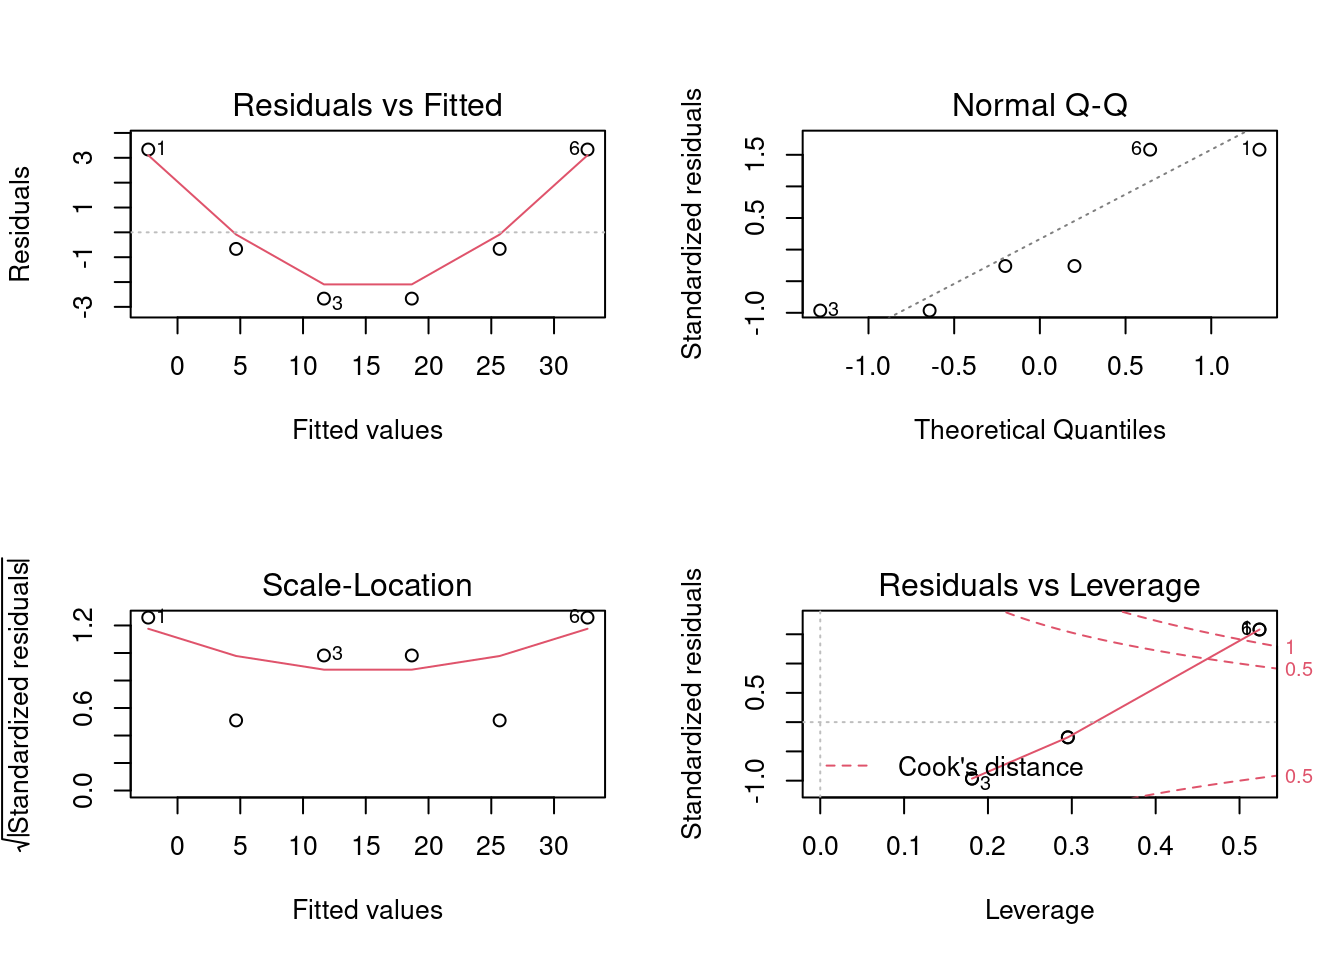
\includegraphics{DASE_files/figure-latex/unnamed-chunk-2-1.pdf}

\begin{Shaded}
\begin{Highlighting}[]
\FunctionTok{help}\NormalTok{(lm)}
\NormalTok{?lm}
\FunctionTok{apropos}\NormalTok{(}\StringTok{"lm"}\NormalTok{)}
\end{Highlighting}
\end{Shaded}

\begin{verbatim}
##  [1] ".colMeans"       ".lm.fit"         "colMeans"        "confint.lm"     
##  [5] "contr.helmert"   "dummy.coef.lm"   "glm"             "glm.control"    
##  [9] "glm.fit"         "KalmanForecast"  "KalmanLike"      "KalmanRun"      
## [13] "KalmanSmooth"    "kappa.lm"        "lm"              "lm_1"           
## [17] "lm.fit"          "lm.influence"    "lm.wfit"         "model.matrix.lm"
## [21] "nlm"             "nlminb"          "predict.glm"     "predict.lm"     
## [25] "residuals.glm"   "residuals.lm"    "summary.glm"     "summary.lm"
\end{verbatim}

\begin{Shaded}
\begin{Highlighting}[]
\FunctionTok{example}\NormalTok{(lm)}
\end{Highlighting}
\end{Shaded}

\begin{verbatim}
## 
## lm> require(graphics)
## 
## lm> ## Annette Dobson (1990) "An Introduction to Generalized Linear Models".
## lm> ## Page 9: Plant Weight Data.
## lm> ctl <- c(4.17,5.58,5.18,6.11,4.50,4.61,5.17,4.53,5.33,5.14)
## 
## lm> trt <- c(4.81,4.17,4.41,3.59,5.87,3.83,6.03,4.89,4.32,4.69)
## 
## lm> group <- gl(2, 10, 20, labels = c("Ctl","Trt"))
## 
## lm> weight <- c(ctl, trt)
## 
## lm> lm.D9 <- lm(weight ~ group)
## 
## lm> lm.D90 <- lm(weight ~ group - 1) # omitting intercept
## 
## lm> ## No test: 
## lm> ##D anova(lm.D9)
## lm> ##D summary(lm.D90)
## lm> ## End(No test)
## lm> opar <- par(mfrow = c(2,2), oma = c(0, 0, 1.1, 0))
## 
## lm> plot(lm.D9, las = 1)      # Residuals, Fitted, ...
\end{verbatim}

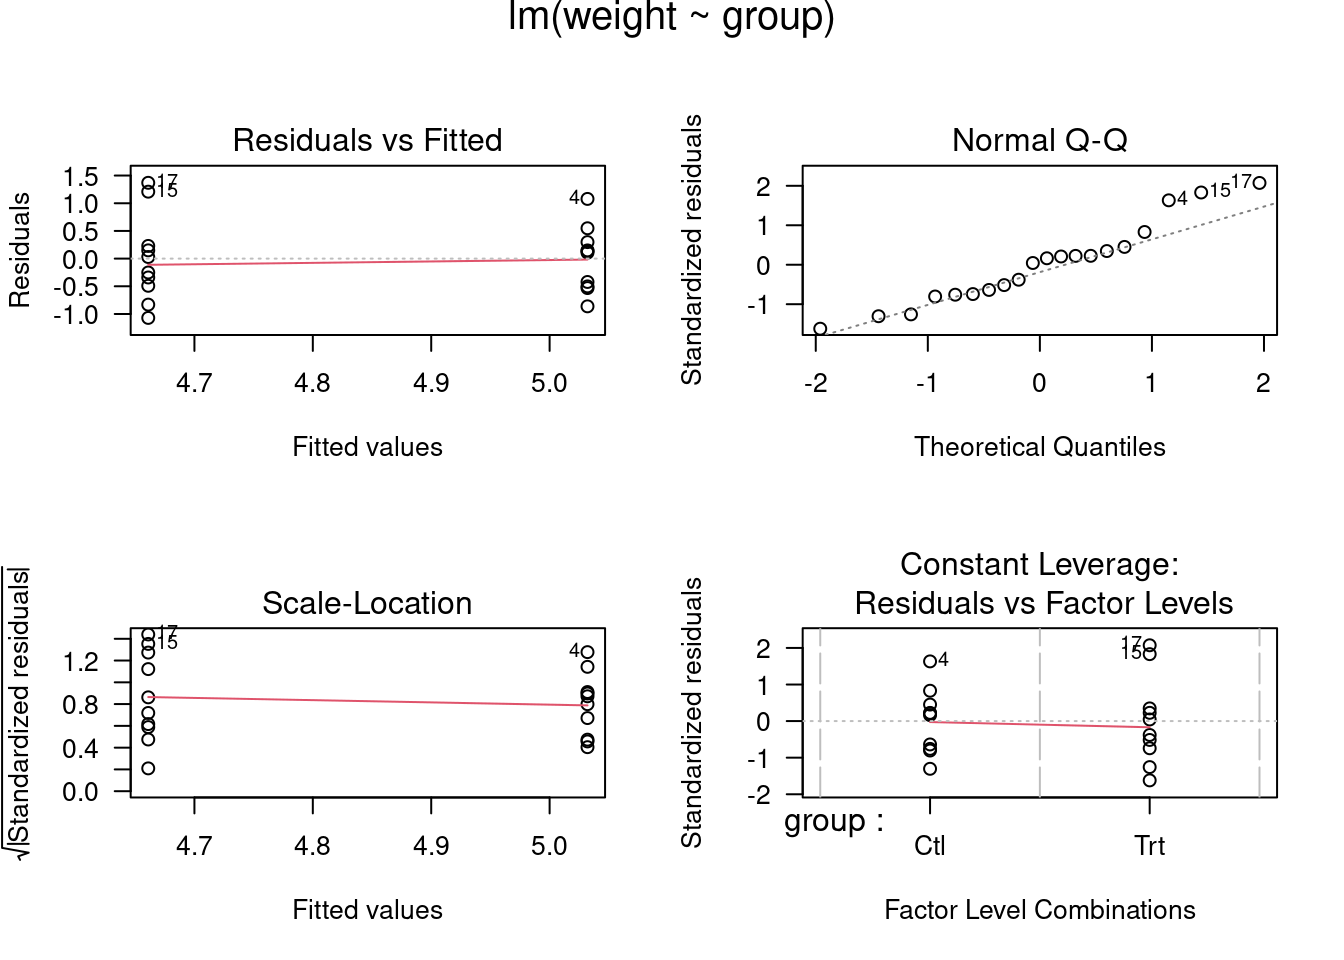
\includegraphics{DASE_files/figure-latex/unnamed-chunk-2-2.pdf}

\begin{verbatim}
## 
## lm> par(opar)
## 
## lm> ## Don't show: 
## lm> ## model frame :
## lm> stopifnot(identical(lm(weight ~ group, method = "model.frame"),
## lm+                     model.frame(lm.D9)))
## 
## lm> ## End(Don't show)
## lm> ### less simple examples in "See Also" above
## lm> 
## lm> 
## lm>
\end{verbatim}

\begin{itemize}
\item
  R script. \# A file with R commands \texttt{\#\ comments} \texttt{source("filewithcommands.R")} \texttt{sink("recordmycommands.lis")} \texttt{savehistory()}
\item
  From command line:

  \begin{itemize}
  \tightlist
  \item
    Rscript\\
  \item
    Rscript file with \texttt{-e} (e.g.~\texttt{Rscript\ -e\ 2+2})\\
  \item
    To exit R: \texttt{quit()}
  \end{itemize}
\item
  Variables. R is case sensitive
\end{itemize}

\begin{Shaded}
\begin{Highlighting}[]
\NormalTok{var1 }\OtherTok{\textless{}{-}} \DecValTok{1}\SpecialCharTok{:}\DecValTok{10}
\NormalTok{vAr1 }\OtherTok{\textless{}{-}} \DecValTok{11}\SpecialCharTok{:}\DecValTok{20}
\NormalTok{var1}
\end{Highlighting}
\end{Shaded}

\begin{verbatim}
##  [1]  1  2  3  4  5  6  7  8  9 10
\end{verbatim}

\begin{Shaded}
\begin{Highlighting}[]
\NormalTok{vAr1 }
\end{Highlighting}
\end{Shaded}

\begin{verbatim}
##  [1] 11 12 13 14 15 16 17 18 19 20
\end{verbatim}

\begin{itemize}
\item
  Operators

  \begin{itemize}
  \tightlist
  \item
    assign operator \texttt{\textless{}-}\\
  \item
    sequence operator, for example: \texttt{mynums\ \textless{}-\ 0:20}
  \item
    arithmetic operators: + - = / \^{} \%/\% (integer division) \%\% (modulus operator)
  \end{itemize}
\item
  The workspace. Objects.

  \begin{itemize}
  \tightlist
  \item
    \texttt{ls()} \texttt{objects()} \texttt{ls.str()} lists and describes the objects\\
  \item
    \texttt{rm(x)} delete a variable. E.g., \texttt{rm(totalCost)}
  \item
    \texttt{s.str()}
  \item
    \texttt{objects()}
  \item
    \texttt{str()} The structure function provides information about the variable
  \end{itemize}
\item
  RStudio, RCommander and RKWard are the well-known IDEs for R (more later).
\end{itemize}

\begin{center}\rule{0.5\linewidth}{0.5pt}\end{center}

\begin{itemize}
\item
  Four \# (`\#\#\#\#') create an \emph{environment} in RStudio. An environment binds a set of names to a set of values. You can think of an environment as a bag of names.

  \begin{itemize}
  \tightlist
  \item
    \href{http://adv-r.had.co.nz/Environments.html\#env-basics}{Environment basics}
  \end{itemize}
\end{itemize}

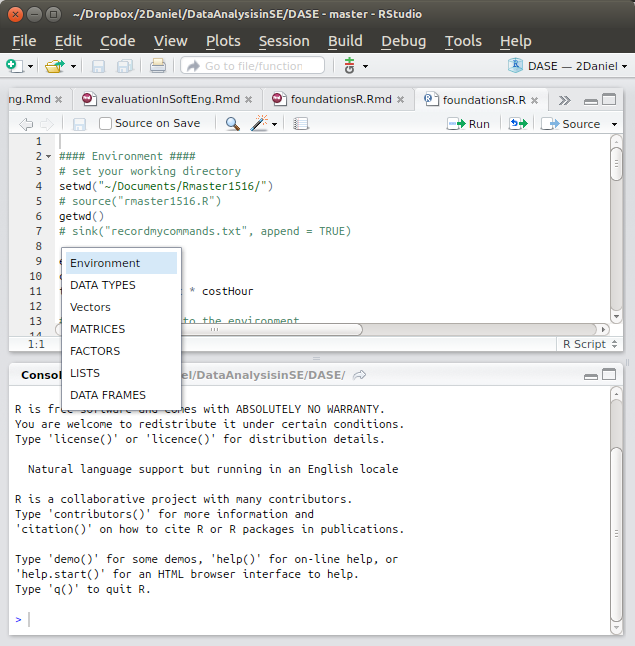
\includegraphics[width=0.75\linewidth]{figures/environments}

Working directories:

\begin{Shaded}
\begin{Highlighting}[]
\CommentTok{\# set your working directory}
\CommentTok{\# setwd("\textasciitilde{}/workingDir/")}
\FunctionTok{getwd}\NormalTok{()}
\end{Highlighting}
\end{Shaded}

\begin{verbatim}
## [1] "/home/drg/Projects/DASE"
\end{verbatim}

\begin{Shaded}
\begin{Highlighting}[]
\CommentTok{\# record R commands:}
\CommentTok{\# sink("recordmycommands.txt", append = TRUE)}
\end{Highlighting}
\end{Shaded}

\begin{center}\rule{0.5\linewidth}{0.5pt}\end{center}

\hypertarget{basic-data-types}{%
\section{Basic Data Types}\label{basic-data-types}}

\begin{itemize}
\item
  \texttt{class(\ )}
\item
  logical: \texttt{TRUE}, \texttt{FALSE}
\item
  numeric, integer:

  \begin{itemize}
  \tightlist
  \item
    \texttt{is.numeric(\ \ )}
  \item
    \texttt{is.integer(\ \ )}\strut \\
  \end{itemize}
\item
  \texttt{character}
\end{itemize}

Examples:

\begin{Shaded}
\begin{Highlighting}[]
\ConstantTok{TRUE}
\end{Highlighting}
\end{Shaded}

\begin{verbatim}
## [1] TRUE
\end{verbatim}

\begin{Shaded}
\begin{Highlighting}[]
\FunctionTok{class}\NormalTok{(}\ConstantTok{TRUE}\NormalTok{)}
\end{Highlighting}
\end{Shaded}

\begin{verbatim}
## [1] "logical"
\end{verbatim}

\begin{Shaded}
\begin{Highlighting}[]
\ConstantTok{FALSE}
\end{Highlighting}
\end{Shaded}

\begin{verbatim}
## [1] FALSE
\end{verbatim}

\begin{Shaded}
\begin{Highlighting}[]
\ConstantTok{NA}  \CommentTok{\# missing}
\end{Highlighting}
\end{Shaded}

\begin{verbatim}
## [1] NA
\end{verbatim}

\begin{Shaded}
\begin{Highlighting}[]
\FunctionTok{class}\NormalTok{(}\ConstantTok{NA}\NormalTok{)}
\end{Highlighting}
\end{Shaded}

\begin{verbatim}
## [1] "logical"
\end{verbatim}

\begin{Shaded}
\begin{Highlighting}[]
\NormalTok{T}
\end{Highlighting}
\end{Shaded}

\begin{verbatim}
## [1] TRUE
\end{verbatim}

\begin{Shaded}
\begin{Highlighting}[]
\NormalTok{F}
\end{Highlighting}
\end{Shaded}

\begin{verbatim}
## [1] FALSE
\end{verbatim}

\begin{Shaded}
\begin{Highlighting}[]
\ConstantTok{NaN}
\end{Highlighting}
\end{Shaded}

\begin{verbatim}
## [1] NaN
\end{verbatim}

\begin{Shaded}
\begin{Highlighting}[]
\FunctionTok{class}\NormalTok{(}\ConstantTok{NaN}\NormalTok{)}
\end{Highlighting}
\end{Shaded}

\begin{verbatim}
## [1] "numeric"
\end{verbatim}

\begin{Shaded}
\begin{Highlighting}[]
\CommentTok{\# numeric data type}
\DecValTok{2}
\end{Highlighting}
\end{Shaded}

\begin{verbatim}
## [1] 2
\end{verbatim}

\begin{Shaded}
\begin{Highlighting}[]
\FunctionTok{class}\NormalTok{(}\DecValTok{2}\NormalTok{)}
\end{Highlighting}
\end{Shaded}

\begin{verbatim}
## [1] "numeric"
\end{verbatim}

\begin{Shaded}
\begin{Highlighting}[]
\FloatTok{2.5}
\end{Highlighting}
\end{Shaded}

\begin{verbatim}
## [1] 2.5
\end{verbatim}

\begin{Shaded}
\begin{Highlighting}[]
\NormalTok{2L  }\CommentTok{\# integer}
\end{Highlighting}
\end{Shaded}

\begin{verbatim}
## [1] 2
\end{verbatim}

\begin{Shaded}
\begin{Highlighting}[]
\FunctionTok{class}\NormalTok{(2L)}
\end{Highlighting}
\end{Shaded}

\begin{verbatim}
## [1] "integer"
\end{verbatim}

\begin{Shaded}
\begin{Highlighting}[]
\FunctionTok{is.numeric}\NormalTok{(}\DecValTok{2}\NormalTok{)}
\end{Highlighting}
\end{Shaded}

\begin{verbatim}
## [1] TRUE
\end{verbatim}

\begin{Shaded}
\begin{Highlighting}[]
\FunctionTok{is.numeric}\NormalTok{(2L)}
\end{Highlighting}
\end{Shaded}

\begin{verbatim}
## [1] TRUE
\end{verbatim}

\begin{Shaded}
\begin{Highlighting}[]
\FunctionTok{is.integer}\NormalTok{(}\DecValTok{2}\NormalTok{)}
\end{Highlighting}
\end{Shaded}

\begin{verbatim}
## [1] FALSE
\end{verbatim}

\begin{Shaded}
\begin{Highlighting}[]
\FunctionTok{is.integer}\NormalTok{(2L)}
\end{Highlighting}
\end{Shaded}

\begin{verbatim}
## [1] TRUE
\end{verbatim}

\begin{Shaded}
\begin{Highlighting}[]
\FunctionTok{is.numeric}\NormalTok{(}\ConstantTok{NaN}\NormalTok{)}
\end{Highlighting}
\end{Shaded}

\begin{verbatim}
## [1] TRUE
\end{verbatim}

\begin{itemize}
\item
  data type coercion:

  \begin{itemize}
  \tightlist
  \item
    \texttt{as.numeric(\ \ )}
  \item
    \texttt{as.character(\ \ )}\strut \\
  \item
    \texttt{as.integer(\ \ )}
  \end{itemize}
\end{itemize}

Examples:

\begin{Shaded}
\begin{Highlighting}[]
\NormalTok{truenum }\OtherTok{\textless{}{-}} \FunctionTok{as.numeric}\NormalTok{(}\ConstantTok{TRUE}\NormalTok{)}
\NormalTok{truenum}
\end{Highlighting}
\end{Shaded}

\begin{verbatim}
## [1] 1
\end{verbatim}

\begin{Shaded}
\begin{Highlighting}[]
\FunctionTok{class}\NormalTok{(truenum)}
\end{Highlighting}
\end{Shaded}

\begin{verbatim}
## [1] "numeric"
\end{verbatim}

\begin{Shaded}
\begin{Highlighting}[]
\NormalTok{falsenum }\OtherTok{\textless{}{-}} \FunctionTok{as.numeric}\NormalTok{(}\ConstantTok{FALSE}\NormalTok{)}
\NormalTok{falsenum}
\end{Highlighting}
\end{Shaded}

\begin{verbatim}
## [1] 0
\end{verbatim}

\begin{Shaded}
\begin{Highlighting}[]
\NormalTok{num2char }\OtherTok{\textless{}{-}} \FunctionTok{as.character}\NormalTok{(}\DecValTok{55}\NormalTok{)}
\NormalTok{num2char}
\end{Highlighting}
\end{Shaded}

\begin{verbatim}
## [1] "55"
\end{verbatim}

\begin{Shaded}
\begin{Highlighting}[]
\NormalTok{char2num  }\OtherTok{\textless{}{-}} \FunctionTok{as.numeric}\NormalTok{(}\StringTok{"55.3"}\NormalTok{)}

\NormalTok{char2int  }\OtherTok{\textless{}{-}} \FunctionTok{as.integer}\NormalTok{(}\StringTok{"55.3"}\NormalTok{)}
\end{Highlighting}
\end{Shaded}

\hypertarget{mising-values}{%
\subsection{Mising values}\label{mising-values}}

\begin{itemize}
\tightlist
\item
  \texttt{NA} stands for Not Available, which is not a number as well. It applies to missing values.
\item
  \texttt{NaN} means `Not a Number'
\end{itemize}

Examples:

\begin{Shaded}
\begin{Highlighting}[]
\ConstantTok{NA} \SpecialCharTok{+} \DecValTok{1}
\end{Highlighting}
\end{Shaded}

\begin{verbatim}
## [1] NA
\end{verbatim}

\begin{Shaded}
\begin{Highlighting}[]
\FunctionTok{mean}\NormalTok{(}\FunctionTok{c}\NormalTok{(}\DecValTok{5}\NormalTok{,}\ConstantTok{NA}\NormalTok{,}\DecValTok{7}\NormalTok{))}
\end{Highlighting}
\end{Shaded}

\begin{verbatim}
## [1] NA
\end{verbatim}

\begin{Shaded}
\begin{Highlighting}[]
\FunctionTok{mean}\NormalTok{(}\FunctionTok{c}\NormalTok{(}\DecValTok{5}\NormalTok{,}\ConstantTok{NA}\NormalTok{,}\DecValTok{7}\NormalTok{), }\AttributeTok{na.rm=}\ConstantTok{TRUE}\NormalTok{)  }\CommentTok{\# some functions allow to remove NAs}
\end{Highlighting}
\end{Shaded}

\begin{verbatim}
## [1] 6
\end{verbatim}

\begin{center}\rule{0.5\linewidth}{0.5pt}\end{center}

\hypertarget{vectors}{%
\section{Vectors}\label{vectors}}

Examples:

\begin{Shaded}
\begin{Highlighting}[]
\NormalTok{phases }\OtherTok{\textless{}{-}} \FunctionTok{c}\NormalTok{(}\StringTok{"reqs"}\NormalTok{, }\StringTok{"dev"}\NormalTok{, }\StringTok{"test1"}\NormalTok{, }\StringTok{"test2"}\NormalTok{, }\StringTok{"maint"}\NormalTok{)}
\FunctionTok{str}\NormalTok{(phases)}
\end{Highlighting}
\end{Shaded}

\begin{verbatim}
##  chr [1:5] "reqs" "dev" "test1" "test2" "maint"
\end{verbatim}

\begin{Shaded}
\begin{Highlighting}[]
\FunctionTok{is.vector}\NormalTok{(phases)}
\end{Highlighting}
\end{Shaded}

\begin{verbatim}
## [1] TRUE
\end{verbatim}

\begin{Shaded}
\begin{Highlighting}[]
\NormalTok{thevalues }\OtherTok{\textless{}{-}} \FunctionTok{c}\NormalTok{(}\DecValTok{15}\NormalTok{, }\DecValTok{60}\NormalTok{, }\DecValTok{30}\NormalTok{, }\DecValTok{35}\NormalTok{, }\DecValTok{22}\NormalTok{)}
\FunctionTok{names}\NormalTok{(thevalues) }\OtherTok{\textless{}{-}}\NormalTok{ phases}
\FunctionTok{str}\NormalTok{(thevalues)}
\end{Highlighting}
\end{Shaded}

\begin{verbatim}
##  Named num [1:5] 15 60 30 35 22
##  - attr(*, "names")= chr [1:5] "reqs" "dev" "test1" "test2" ...
\end{verbatim}

\begin{Shaded}
\begin{Highlighting}[]
\NormalTok{thevalues}
\end{Highlighting}
\end{Shaded}

\begin{verbatim}
##  reqs   dev test1 test2 maint 
##    15    60    30    35    22
\end{verbatim}

A single value is a vector! Example:

\begin{Shaded}
\begin{Highlighting}[]
\NormalTok{aphase }\OtherTok{\textless{}{-}} \DecValTok{44}
\FunctionTok{is.vector}\NormalTok{(aphase)}
\end{Highlighting}
\end{Shaded}

\begin{verbatim}
## [1] TRUE
\end{verbatim}

\begin{Shaded}
\begin{Highlighting}[]
\FunctionTok{length}\NormalTok{(aphase)}
\end{Highlighting}
\end{Shaded}

\begin{verbatim}
## [1] 1
\end{verbatim}

\begin{Shaded}
\begin{Highlighting}[]
\FunctionTok{length}\NormalTok{(thevalues)}
\end{Highlighting}
\end{Shaded}

\begin{verbatim}
## [1] 5
\end{verbatim}

\hypertarget{coercion-for-vectors}{%
\subsection{Coercion for vectors}\label{coercion-for-vectors}}

\begin{Shaded}
\begin{Highlighting}[]
\NormalTok{thevalues1 }\OtherTok{\textless{}{-}} \FunctionTok{c}\NormalTok{(}\DecValTok{15}\NormalTok{, }\DecValTok{60}\NormalTok{, }\StringTok{"30"}\NormalTok{, }\DecValTok{35}\NormalTok{, }\DecValTok{22}\NormalTok{)}
\FunctionTok{class}\NormalTok{(thevalues1)}
\end{Highlighting}
\end{Shaded}

\begin{verbatim}
## [1] "character"
\end{verbatim}

\begin{Shaded}
\begin{Highlighting}[]
\NormalTok{thevalues1}
\end{Highlighting}
\end{Shaded}

\begin{verbatim}
## [1] "15" "60" "30" "35" "22"
\end{verbatim}

\begin{Shaded}
\begin{Highlighting}[]
\CommentTok{\# \textless{}{-}  is equivalent to   assign ( )}

\FunctionTok{assign}\NormalTok{(}\StringTok{"costs"}\NormalTok{, }\FunctionTok{c}\NormalTok{(}\DecValTok{50}\NormalTok{, }\DecValTok{100}\NormalTok{, }\DecValTok{30}\NormalTok{))}
\end{Highlighting}
\end{Shaded}

\hypertarget{vector-arithmetic}{%
\subsection{Vector arithmetic}\label{vector-arithmetic}}

The operation is carried out in all the elements of the vector. For example:

\begin{Shaded}
\begin{Highlighting}[]
\FunctionTok{assign}\NormalTok{(}\StringTok{"costs"}\NormalTok{, }\FunctionTok{c}\NormalTok{(}\DecValTok{50}\NormalTok{, }\DecValTok{100}\NormalTok{, }\DecValTok{30}\NormalTok{))}
\NormalTok{costs}\SpecialCharTok{/}\DecValTok{3}
\end{Highlighting}
\end{Shaded}

\begin{verbatim}
## [1] 16.66667 33.33333 10.00000
\end{verbatim}

\begin{Shaded}
\begin{Highlighting}[]
\NormalTok{costs }\SpecialCharTok{{-}} \DecValTok{5}
\end{Highlighting}
\end{Shaded}

\begin{verbatim}
## [1] 45 95 25
\end{verbatim}

\begin{Shaded}
\begin{Highlighting}[]
\NormalTok{costs }\OtherTok{\textless{}{-}}\NormalTok{ costs }\SpecialCharTok{{-}} \DecValTok{5}

\NormalTok{incomes }\OtherTok{\textless{}{-}} \FunctionTok{c}\NormalTok{(}\DecValTok{200}\NormalTok{, }\DecValTok{800}\NormalTok{, }\DecValTok{10}\NormalTok{)}
\NormalTok{earnings }\OtherTok{\textless{}{-}}\NormalTok{ incomes }\SpecialCharTok{{-}}\NormalTok{ costs}
\FunctionTok{sum}\NormalTok{(earnings)}
\end{Highlighting}
\end{Shaded}

\begin{verbatim}
## [1] 845
\end{verbatim}

\begin{Shaded}
\begin{Highlighting}[]
\CommentTok{\# R recycles values in vectors!}
\NormalTok{vector1 }\OtherTok{\textless{}{-}} \FunctionTok{c}\NormalTok{(}\DecValTok{1}\NormalTok{,}\DecValTok{2}\NormalTok{,}\DecValTok{3}\NormalTok{)}
\NormalTok{vector2 }\OtherTok{\textless{}{-}} \FunctionTok{c}\NormalTok{(}\DecValTok{10}\NormalTok{,}\DecValTok{11}\NormalTok{,}\DecValTok{12}\NormalTok{,}\DecValTok{13}\NormalTok{,}\DecValTok{14}\NormalTok{,}\DecValTok{15}\NormalTok{,}\DecValTok{16}\NormalTok{)}
\NormalTok{vector1 }\SpecialCharTok{+}\NormalTok{ vector2}
\end{Highlighting}
\end{Shaded}

\begin{verbatim}
## Warning in vector1 + vector2: longer object length is not a multiple of shorter
## object length
\end{verbatim}

\begin{verbatim}
## [1] 11 13 15 14 16 18 17
\end{verbatim}

Subsetting vectors

\begin{Shaded}
\begin{Highlighting}[]
\DocumentationTok{\#\#\# Subsetting vectors  []}

\NormalTok{phase1 }\OtherTok{\textless{}{-}}\NormalTok{ phases[}\DecValTok{1}\NormalTok{]}
\NormalTok{phase1}
\end{Highlighting}
\end{Shaded}

\begin{verbatim}
## [1] "reqs"
\end{verbatim}

\begin{Shaded}
\begin{Highlighting}[]
\NormalTok{phase3 }\OtherTok{\textless{}{-}}\NormalTok{ phases[}\DecValTok{3}\NormalTok{]}
\NormalTok{phase3}
\end{Highlighting}
\end{Shaded}

\begin{verbatim}
## [1] "test1"
\end{verbatim}

\begin{Shaded}
\begin{Highlighting}[]
\NormalTok{thevalues[phase1]}
\end{Highlighting}
\end{Shaded}

\begin{verbatim}
## reqs 
##   15
\end{verbatim}

\begin{Shaded}
\begin{Highlighting}[]
\NormalTok{thevalues[}\StringTok{"reqs"}\NormalTok{]}
\end{Highlighting}
\end{Shaded}

\begin{verbatim}
## reqs 
##   15
\end{verbatim}

\begin{Shaded}
\begin{Highlighting}[]
\NormalTok{testphases }\OtherTok{\textless{}{-}}\NormalTok{ phases[}\FunctionTok{c}\NormalTok{(}\DecValTok{3}\NormalTok{,}\DecValTok{4}\NormalTok{)]}
\NormalTok{thevalues[testphases]}
\end{Highlighting}
\end{Shaded}

\begin{verbatim}
## test1 test2 
##    30    35
\end{verbatim}

\begin{Shaded}
\begin{Highlighting}[]
\DocumentationTok{\#\#\# Negative indexes}

\NormalTok{phases1 }\OtherTok{\textless{}{-}}\NormalTok{ phases[}\SpecialCharTok{{-}}\DecValTok{5}\NormalTok{]}
\NormalTok{phases}
\end{Highlighting}
\end{Shaded}

\begin{verbatim}
## [1] "reqs"  "dev"   "test1" "test2" "maint"
\end{verbatim}

\begin{Shaded}
\begin{Highlighting}[]
\NormalTok{phases1}
\end{Highlighting}
\end{Shaded}

\begin{verbatim}
## [1] "reqs"  "dev"   "test1" "test2"
\end{verbatim}

\begin{Shaded}
\begin{Highlighting}[]
\CommentTok{\#phases2 \textless{}{-} phases[{-}testphases] \#\# error in argument}
\NormalTok{phases2 }\OtherTok{\textless{}{-}}\NormalTok{ phases[}\SpecialCharTok{{-}}\FunctionTok{c}\NormalTok{(}\DecValTok{3}\NormalTok{,}\DecValTok{4}\NormalTok{)]}
\NormalTok{phases2}
\end{Highlighting}
\end{Shaded}

\begin{verbatim}
## [1] "reqs"  "dev"   "maint"
\end{verbatim}

\begin{Shaded}
\begin{Highlighting}[]
\DocumentationTok{\#\#\# subset using logical vector}

\NormalTok{phases3 }\OtherTok{\textless{}{-}}\NormalTok{ phases[}\FunctionTok{c}\NormalTok{(}\ConstantTok{FALSE}\NormalTok{, }\ConstantTok{TRUE}\NormalTok{, }\ConstantTok{TRUE}\NormalTok{, }\ConstantTok{FALSE}\NormalTok{)] }\CommentTok{\#recicled first value}
\NormalTok{phases3}
\end{Highlighting}
\end{Shaded}

\begin{verbatim}
## [1] "dev"   "test1"
\end{verbatim}

\begin{Shaded}
\begin{Highlighting}[]
\NormalTok{selectionv }\OtherTok{\textless{}{-}} \FunctionTok{c}\NormalTok{(}\ConstantTok{FALSE}\NormalTok{, }\ConstantTok{TRUE}\NormalTok{, }\ConstantTok{TRUE}\NormalTok{, }\ConstantTok{FALSE}\NormalTok{)}
\NormalTok{phases3 }\OtherTok{\textless{}{-}}\NormalTok{ phases[selectionv]}
\NormalTok{phases3}
\end{Highlighting}
\end{Shaded}

\begin{verbatim}
## [1] "dev"   "test1"
\end{verbatim}

\begin{Shaded}
\begin{Highlighting}[]
\NormalTok{selectionvec2 }\OtherTok{\textless{}{-}} \FunctionTok{c}\NormalTok{(}\ConstantTok{TRUE}\NormalTok{, }\ConstantTok{FALSE}\NormalTok{)}

\NormalTok{thevalues2 }\OtherTok{\textless{}{-}}\NormalTok{ thevalues[selectionvec2]}
\NormalTok{thevalues2}
\end{Highlighting}
\end{Shaded}

\begin{verbatim}
##  reqs test1 maint 
##    15    30    22
\end{verbatim}

\begin{Shaded}
\begin{Highlighting}[]
\DocumentationTok{\#\#\# Generating regular sequences with  \textasciigrave{}:\textasciigrave{} and \textasciigrave{}seq\textasciigrave{}}

\NormalTok{aseqofvalues }\OtherTok{\textless{}{-}} \DecValTok{1}\SpecialCharTok{:}\DecValTok{20}

\NormalTok{aseqofvalues2 }\OtherTok{\textless{}{-}} \FunctionTok{seq}\NormalTok{(}\AttributeTok{from=}\SpecialCharTok{{-}}\DecValTok{3}\NormalTok{, }\AttributeTok{to=}\DecValTok{3}\NormalTok{, }\AttributeTok{by=}\FloatTok{0.5}\NormalTok{ )}
\NormalTok{aseqofvalues2}
\end{Highlighting}
\end{Shaded}

\begin{verbatim}
##  [1] -3.0 -2.5 -2.0 -1.5 -1.0 -0.5  0.0  0.5  1.0  1.5  2.0  2.5  3.0
\end{verbatim}

\begin{Shaded}
\begin{Highlighting}[]
\NormalTok{aseqofvalues3 }\OtherTok{\textless{}{-}} \FunctionTok{seq}\NormalTok{(}\DecValTok{0}\NormalTok{, }\DecValTok{100}\NormalTok{, }\AttributeTok{by=}\DecValTok{10}\NormalTok{)}
\NormalTok{aseqofvalues4 }\OtherTok{\textless{}{-}}\NormalTok{ aseqofvalues3[}\FunctionTok{c}\NormalTok{(}\DecValTok{2}\NormalTok{, }\DecValTok{4}\NormalTok{, }\DecValTok{6}\NormalTok{, }\DecValTok{8}\NormalTok{)]}
\NormalTok{aseqofvalues4}
\end{Highlighting}
\end{Shaded}

\begin{verbatim}
## [1] 10 30 50 70
\end{verbatim}

\begin{Shaded}
\begin{Highlighting}[]
\NormalTok{aseqofvalues4 }\OtherTok{\textless{}{-}}\NormalTok{ aseqofvalues3[}\SpecialCharTok{{-}}\FunctionTok{c}\NormalTok{(}\DecValTok{2}\NormalTok{, }\DecValTok{4}\NormalTok{, }\DecValTok{6}\NormalTok{, }\DecValTok{8}\NormalTok{)]}
\NormalTok{aseqofvalues4}
\end{Highlighting}
\end{Shaded}

\begin{verbatim}
## [1]   0  20  40  60  80  90 100
\end{verbatim}

\begin{Shaded}
\begin{Highlighting}[]
\NormalTok{aseqofvalues3[}\FunctionTok{c}\NormalTok{(}\DecValTok{1}\NormalTok{,}\DecValTok{2}\NormalTok{)] }\OtherTok{\textless{}{-}} \FunctionTok{c}\NormalTok{(}\DecValTok{666}\NormalTok{,}\DecValTok{888}\NormalTok{)}
\NormalTok{aseqofvalues3}
\end{Highlighting}
\end{Shaded}

\begin{verbatim}
##  [1] 666 888  20  30  40  50  60  70  80  90 100
\end{verbatim}

\begin{Shaded}
\begin{Highlighting}[]
\DocumentationTok{\#\#\# Logical values in vectors TRUE/FALSE}

\NormalTok{aseqofvalues3 }\SpecialCharTok{\textgreater{}} \DecValTok{50}
\end{Highlighting}
\end{Shaded}

\begin{verbatim}
##  [1]  TRUE  TRUE FALSE FALSE FALSE FALSE  TRUE  TRUE  TRUE  TRUE  TRUE
\end{verbatim}

\begin{Shaded}
\begin{Highlighting}[]
\NormalTok{aseqofvalues5 }\OtherTok{\textless{}{-}}\NormalTok{ aseqofvalues3[aseqofvalues3 }\SpecialCharTok{\textgreater{}} \DecValTok{50}\NormalTok{]}
\NormalTok{aseqofvalues5}
\end{Highlighting}
\end{Shaded}

\begin{verbatim}
## [1] 666 888  60  70  80  90 100
\end{verbatim}

\begin{Shaded}
\begin{Highlighting}[]
\NormalTok{aseqofvalues6 }\OtherTok{\textless{}{-}}\NormalTok{ aseqofvalues3[}\SpecialCharTok{!}\NormalTok{(aseqofvalues3 }\SpecialCharTok{\textgreater{}} \DecValTok{50}\NormalTok{)]}
\NormalTok{aseqofvalues6}
\end{Highlighting}
\end{Shaded}

\begin{verbatim}
## [1] 20 30 40 50
\end{verbatim}

\begin{Shaded}
\begin{Highlighting}[]
\DocumentationTok{\#\#\# Comparison functions}

\NormalTok{aseqofvalues7 }\OtherTok{\textless{}{-}}\NormalTok{ aseqofvalues3[aseqofvalues3 }\SpecialCharTok{==} \DecValTok{50}\NormalTok{]}
\NormalTok{aseqofvalues7}
\end{Highlighting}
\end{Shaded}

\begin{verbatim}
## [1] 50
\end{verbatim}

\begin{Shaded}
\begin{Highlighting}[]
\NormalTok{aseqofvalues8 }\OtherTok{\textless{}{-}}\NormalTok{ aseqofvalues3[aseqofvalues3 }\SpecialCharTok{==} \DecValTok{22}\NormalTok{]}
\NormalTok{aseqofvalues8}
\end{Highlighting}
\end{Shaded}

\begin{verbatim}
## numeric(0)
\end{verbatim}

\begin{Shaded}
\begin{Highlighting}[]
\NormalTok{aseqofvalues9 }\OtherTok{\textless{}{-}}\NormalTok{ aseqofvalues3[aseqofvalues3 }\SpecialCharTok{!=} \DecValTok{50}\NormalTok{]}
\NormalTok{aseqofvalues9}
\end{Highlighting}
\end{Shaded}

\begin{verbatim}
##  [1] 666 888  20  30  40  60  70  80  90 100
\end{verbatim}

\begin{Shaded}
\begin{Highlighting}[]
\NormalTok{logicalcond }\OtherTok{\textless{}{-}}\NormalTok{ aseqofvalues3 }\SpecialCharTok{\textgreater{}=} \DecValTok{50}
\NormalTok{aseqofvalues10 }\OtherTok{\textless{}{-}}\NormalTok{ aseqofvalues3[logicalcond]}
\NormalTok{aseqofvalues10}
\end{Highlighting}
\end{Shaded}

\begin{verbatim}
## [1] 666 888  50  60  70  80  90 100
\end{verbatim}

\begin{Shaded}
\begin{Highlighting}[]
\DocumentationTok{\#\#\# Remove Missing Values (NAs)}

\NormalTok{aseqofvalues3[}\FunctionTok{c}\NormalTok{(}\DecValTok{1}\NormalTok{,}\DecValTok{2}\NormalTok{)] }\OtherTok{\textless{}{-}} \FunctionTok{c}\NormalTok{(}\ConstantTok{NA}\NormalTok{,}\ConstantTok{NA}\NormalTok{)}
\NormalTok{aseqofvalues3}
\end{Highlighting}
\end{Shaded}

\begin{verbatim}
##  [1]  NA  NA  20  30  40  50  60  70  80  90 100
\end{verbatim}

\begin{Shaded}
\begin{Highlighting}[]
\NormalTok{aseqofvalues3 }\OtherTok{\textless{}{-}}\NormalTok{ aseqofvalues3[}\SpecialCharTok{!}\FunctionTok{is.na}\NormalTok{(aseqofvalues3)]}
\NormalTok{aseqofvalues3}
\end{Highlighting}
\end{Shaded}

\begin{verbatim}
## [1]  20  30  40  50  60  70  80  90 100
\end{verbatim}

\begin{center}\rule{0.5\linewidth}{0.5pt}\end{center}

\hypertarget{arrays-and-matrices}{%
\section{Arrays and Matrices}\label{arrays-and-matrices}}

Matrices are actually long vectors.

\begin{Shaded}
\begin{Highlighting}[]
\NormalTok{mymat }\OtherTok{\textless{}{-}} \FunctionTok{matrix}\NormalTok{(}\DecValTok{1}\SpecialCharTok{:}\DecValTok{12}\NormalTok{, }\AttributeTok{nrow =}\DecValTok{2}\NormalTok{)}
\NormalTok{mymat}
\end{Highlighting}
\end{Shaded}

\begin{verbatim}
##      [,1] [,2] [,3] [,4] [,5] [,6]
## [1,]    1    3    5    7    9   11
## [2,]    2    4    6    8   10   12
\end{verbatim}

\begin{Shaded}
\begin{Highlighting}[]
\NormalTok{mymat }\OtherTok{\textless{}{-}} \FunctionTok{matrix}\NormalTok{(}\DecValTok{1}\SpecialCharTok{:}\DecValTok{12}\NormalTok{, }\AttributeTok{ncol =}\DecValTok{3}\NormalTok{)}
\NormalTok{mymat}
\end{Highlighting}
\end{Shaded}

\begin{verbatim}
##      [,1] [,2] [,3]
## [1,]    1    5    9
## [2,]    2    6   10
## [3,]    3    7   11
## [4,]    4    8   12
\end{verbatim}

\begin{Shaded}
\begin{Highlighting}[]
\NormalTok{mymat }\OtherTok{\textless{}{-}} \FunctionTok{matrix}\NormalTok{(}\DecValTok{1}\SpecialCharTok{:}\DecValTok{12}\NormalTok{, }\AttributeTok{nrow=}\DecValTok{2}\NormalTok{, }\AttributeTok{byrow =} \ConstantTok{TRUE}\NormalTok{)}
\NormalTok{mymat}
\end{Highlighting}
\end{Shaded}

\begin{verbatim}
##      [,1] [,2] [,3] [,4] [,5] [,6]
## [1,]    1    2    3    4    5    6
## [2,]    7    8    9   10   11   12
\end{verbatim}

\begin{Shaded}
\begin{Highlighting}[]
\NormalTok{mymat }\OtherTok{\textless{}{-}} \FunctionTok{matrix}\NormalTok{(}\DecValTok{1}\SpecialCharTok{:}\DecValTok{12}\NormalTok{, }\AttributeTok{nrow=}\DecValTok{3}\NormalTok{, }\AttributeTok{ncol=}\DecValTok{4}\NormalTok{)}
\NormalTok{mymat}
\end{Highlighting}
\end{Shaded}

\begin{verbatim}
##      [,1] [,2] [,3] [,4]
## [1,]    1    4    7   10
## [2,]    2    5    8   11
## [3,]    3    6    9   12
\end{verbatim}

\begin{Shaded}
\begin{Highlighting}[]
\NormalTok{mymat }\OtherTok{\textless{}{-}} \FunctionTok{matrix}\NormalTok{(}\DecValTok{1}\SpecialCharTok{:}\DecValTok{12}\NormalTok{, }\AttributeTok{nrow=}\DecValTok{3}\NormalTok{, }\AttributeTok{ncol=}\DecValTok{4}\NormalTok{, }\AttributeTok{byrow=}\ConstantTok{TRUE}\NormalTok{)}
\NormalTok{mymat}
\end{Highlighting}
\end{Shaded}

\begin{verbatim}
##      [,1] [,2] [,3] [,4]
## [1,]    1    2    3    4
## [2,]    5    6    7    8
## [3,]    9   10   11   12
\end{verbatim}

\begin{Shaded}
\begin{Highlighting}[]
\DocumentationTok{\#\#\# recycling}
\NormalTok{mymat }\OtherTok{\textless{}{-}} \FunctionTok{matrix}\NormalTok{(}\DecValTok{1}\SpecialCharTok{:}\DecValTok{5}\NormalTok{, }\AttributeTok{nrow=}\DecValTok{3}\NormalTok{, }\AttributeTok{ncol=}\DecValTok{4}\NormalTok{, }\AttributeTok{byrow=}\ConstantTok{TRUE}\NormalTok{)}
\end{Highlighting}
\end{Shaded}

\begin{verbatim}
## Warning in matrix(1:5, nrow = 3, ncol = 4, byrow = TRUE): data length [5] is not
## a sub-multiple or multiple of the number of rows [3]
\end{verbatim}

\begin{Shaded}
\begin{Highlighting}[]
\NormalTok{mymat}
\end{Highlighting}
\end{Shaded}

\begin{verbatim}
##      [,1] [,2] [,3] [,4]
## [1,]    1    2    3    4
## [2,]    5    1    2    3
## [3,]    4    5    1    2
\end{verbatim}

\begin{Shaded}
\begin{Highlighting}[]
\DocumentationTok{\#\#\# rbind  cbind}

\FunctionTok{cbind}\NormalTok{(}\DecValTok{1}\SpecialCharTok{:}\DecValTok{3}\NormalTok{, }\DecValTok{1}\SpecialCharTok{:}\DecValTok{3}\NormalTok{)}
\end{Highlighting}
\end{Shaded}

\begin{verbatim}
##      [,1] [,2]
## [1,]    1    1
## [2,]    2    2
## [3,]    3    3
\end{verbatim}

\begin{Shaded}
\begin{Highlighting}[]
\FunctionTok{rbind}\NormalTok{(}\DecValTok{1}\SpecialCharTok{:}\DecValTok{3}\NormalTok{, }\DecValTok{1}\SpecialCharTok{:}\DecValTok{3}\NormalTok{)}
\end{Highlighting}
\end{Shaded}

\begin{verbatim}
##      [,1] [,2] [,3]
## [1,]    1    2    3
## [2,]    1    2    3
\end{verbatim}

\begin{Shaded}
\begin{Highlighting}[]
\NormalTok{mymat }\OtherTok{\textless{}{-}} \FunctionTok{matrix}\NormalTok{(}\DecValTok{1}\NormalTok{)}

\NormalTok{mymat }\OtherTok{\textless{}{-}} \FunctionTok{matrix}\NormalTok{(}\DecValTok{1}\SpecialCharTok{:}\DecValTok{8}\NormalTok{, }\AttributeTok{nrow=}\DecValTok{2}\NormalTok{, }\AttributeTok{ncol=}\DecValTok{4}\NormalTok{, }\AttributeTok{byrow=}\ConstantTok{TRUE}\NormalTok{)}
\NormalTok{mymat}
\end{Highlighting}
\end{Shaded}

\begin{verbatim}
##      [,1] [,2] [,3] [,4]
## [1,]    1    2    3    4
## [2,]    5    6    7    8
\end{verbatim}

\begin{Shaded}
\begin{Highlighting}[]
\FunctionTok{rbind}\NormalTok{(mymat, }\DecValTok{9}\SpecialCharTok{:}\DecValTok{12}\NormalTok{)}
\end{Highlighting}
\end{Shaded}

\begin{verbatim}
##      [,1] [,2] [,3] [,4]
## [1,]    1    2    3    4
## [2,]    5    6    7    8
## [3,]    9   10   11   12
\end{verbatim}

\begin{Shaded}
\begin{Highlighting}[]
\NormalTok{mymat }\OtherTok{\textless{}{-}} \FunctionTok{cbind}\NormalTok{(mymat, }\FunctionTok{c}\NormalTok{(}\DecValTok{5}\NormalTok{,}\DecValTok{9}\NormalTok{))}
\NormalTok{mymat}
\end{Highlighting}
\end{Shaded}

\begin{verbatim}
##      [,1] [,2] [,3] [,4] [,5]
## [1,]    1    2    3    4    5
## [2,]    5    6    7    8    9
\end{verbatim}

\begin{Shaded}
\begin{Highlighting}[]
\NormalTok{mymat  }\OtherTok{\textless{}{-}} \FunctionTok{matrix}\NormalTok{(}\DecValTok{1}\SpecialCharTok{:}\DecValTok{8}\NormalTok{, }\AttributeTok{byrow =} \ConstantTok{TRUE}\NormalTok{, }\AttributeTok{nrow=}\DecValTok{2}\NormalTok{)}
\NormalTok{mymat}
\end{Highlighting}
\end{Shaded}

\begin{verbatim}
##      [,1] [,2] [,3] [,4]
## [1,]    1    2    3    4
## [2,]    5    6    7    8
\end{verbatim}

\begin{Shaded}
\begin{Highlighting}[]
\FunctionTok{rownames}\NormalTok{(mymat) }\OtherTok{\textless{}{-}} \FunctionTok{c}\NormalTok{(}\StringTok{"row1"}\NormalTok{, }\StringTok{"row2"}\NormalTok{)}
\NormalTok{mymat}
\end{Highlighting}
\end{Shaded}

\begin{verbatim}
##      [,1] [,2] [,3] [,4]
## row1    1    2    3    4
## row2    5    6    7    8
\end{verbatim}

\begin{Shaded}
\begin{Highlighting}[]
\FunctionTok{colnames}\NormalTok{(mymat) }\OtherTok{\textless{}{-}} \FunctionTok{c}\NormalTok{(}\StringTok{"col1"}\NormalTok{, }\StringTok{"col2"}\NormalTok{, }\StringTok{"col3"}\NormalTok{, }\StringTok{"col4"}\NormalTok{)}
\NormalTok{mymat}
\end{Highlighting}
\end{Shaded}

\begin{verbatim}
##      col1 col2 col3 col4
## row1    1    2    3    4
## row2    5    6    7    8
\end{verbatim}

\begin{Shaded}
\begin{Highlighting}[]
\NormalTok{mymat2 }\OtherTok{\textless{}{-}} \FunctionTok{matrix}\NormalTok{(}\DecValTok{1}\SpecialCharTok{:}\DecValTok{12}\NormalTok{, }\AttributeTok{byrow=}\ConstantTok{TRUE}\NormalTok{, }\AttributeTok{nrow=}\DecValTok{3}\NormalTok{, }\AttributeTok{dimnames=}\FunctionTok{list}\NormalTok{(}\FunctionTok{c}\NormalTok{(}\StringTok{"row1"}\NormalTok{, }\StringTok{"row2"}\NormalTok{, }\StringTok{"row3"}\NormalTok{),}
                                                         \FunctionTok{c}\NormalTok{(}\StringTok{"col1"}\NormalTok{, }\StringTok{"col2"}\NormalTok{, }\StringTok{"col3"}\NormalTok{, }\StringTok{"col4"}\NormalTok{)))}
\NormalTok{mymat2}
\end{Highlighting}
\end{Shaded}

\begin{verbatim}
##      col1 col2 col3 col4
## row1    1    2    3    4
## row2    5    6    7    8
## row3    9   10   11   12
\end{verbatim}

\begin{Shaded}
\begin{Highlighting}[]
\DocumentationTok{\#\#\# Coercion in Arrays}

\NormalTok{matnum }\OtherTok{\textless{}{-}} \FunctionTok{matrix}\NormalTok{(}\DecValTok{1}\SpecialCharTok{:}\DecValTok{8}\NormalTok{, }\AttributeTok{ncol =} \DecValTok{2}\NormalTok{)}
\NormalTok{matnum}
\end{Highlighting}
\end{Shaded}

\begin{verbatim}
##      [,1] [,2]
## [1,]    1    5
## [2,]    2    6
## [3,]    3    7
## [4,]    4    8
\end{verbatim}

\begin{Shaded}
\begin{Highlighting}[]
\NormalTok{matchar }\OtherTok{\textless{}{-}} \FunctionTok{matrix}\NormalTok{(LETTERS[}\DecValTok{1}\SpecialCharTok{:}\DecValTok{6}\NormalTok{], }\AttributeTok{nrow =} \DecValTok{4}\NormalTok{, }\AttributeTok{ncol =} \DecValTok{3}\NormalTok{)}
\NormalTok{matchar}
\end{Highlighting}
\end{Shaded}

\begin{verbatim}
##      [,1] [,2] [,3]
## [1,] "A"  "E"  "C" 
## [2,] "B"  "F"  "D" 
## [3,] "C"  "A"  "E" 
## [4,] "D"  "B"  "F"
\end{verbatim}

\begin{Shaded}
\begin{Highlighting}[]
\NormalTok{matchars }\OtherTok{\textless{}{-}} \FunctionTok{cbind}\NormalTok{(matnum, matchar)}
\NormalTok{matchars}
\end{Highlighting}
\end{Shaded}

\begin{verbatim}
##      [,1] [,2] [,3] [,4] [,5]
## [1,] "1"  "5"  "A"  "E"  "C" 
## [2,] "2"  "6"  "B"  "F"  "D" 
## [3,] "3"  "7"  "C"  "A"  "E" 
## [4,] "4"  "8"  "D"  "B"  "F"
\end{verbatim}

\begin{Shaded}
\begin{Highlighting}[]
\DocumentationTok{\#\#\# Subsetting  }

\NormalTok{mymat3 }\OtherTok{\textless{}{-}} \FunctionTok{matrix}\NormalTok{(}\FunctionTok{sample}\NormalTok{(}\SpecialCharTok{{-}}\DecValTok{8}\SpecialCharTok{:}\DecValTok{15}\NormalTok{, }\DecValTok{12}\NormalTok{), }\AttributeTok{nrow=}\DecValTok{3}\NormalTok{)  }\CommentTok{\#sample 12 numbers between {-}8 and 15}
\NormalTok{mymat3}
\end{Highlighting}
\end{Shaded}

\begin{verbatim}
##      [,1] [,2] [,3] [,4]
## [1,]    5   13   -5   15
## [2,]    3   -8   12    0
## [3,]   -3    8    4   -1
\end{verbatim}

\begin{Shaded}
\begin{Highlighting}[]
\NormalTok{mymat3[}\DecValTok{2}\NormalTok{,}\DecValTok{3}\NormalTok{]}
\end{Highlighting}
\end{Shaded}

\begin{verbatim}
## [1] 12
\end{verbatim}

\begin{Shaded}
\begin{Highlighting}[]
\NormalTok{mymat3[}\DecValTok{1}\NormalTok{,}\DecValTok{4}\NormalTok{]}
\end{Highlighting}
\end{Shaded}

\begin{verbatim}
## [1] 15
\end{verbatim}

\begin{Shaded}
\begin{Highlighting}[]
\NormalTok{mymat3[}\DecValTok{3}\NormalTok{,]}
\end{Highlighting}
\end{Shaded}

\begin{verbatim}
## [1] -3  8  4 -1
\end{verbatim}

\begin{Shaded}
\begin{Highlighting}[]
\NormalTok{mymat3[,}\DecValTok{4}\NormalTok{]}
\end{Highlighting}
\end{Shaded}

\begin{verbatim}
## [1] 15  0 -1
\end{verbatim}

\begin{Shaded}
\begin{Highlighting}[]
\NormalTok{mymat3[}\DecValTok{5}\NormalTok{] }\CommentTok{\# counts elements by column}
\end{Highlighting}
\end{Shaded}

\begin{verbatim}
## [1] -8
\end{verbatim}

\begin{Shaded}
\begin{Highlighting}[]
\NormalTok{mymat3[}\DecValTok{9}\NormalTok{]}
\end{Highlighting}
\end{Shaded}

\begin{verbatim}
## [1] 4
\end{verbatim}

\begin{Shaded}
\begin{Highlighting}[]
\DocumentationTok{\#\# Subsetting multiple elements}

\NormalTok{mymat3[}\DecValTok{2}\NormalTok{, }\FunctionTok{c}\NormalTok{(}\DecValTok{1}\NormalTok{,}\DecValTok{3}\NormalTok{)]}
\end{Highlighting}
\end{Shaded}

\begin{verbatim}
## [1]  3 12
\end{verbatim}

\begin{Shaded}
\begin{Highlighting}[]
\NormalTok{mymat3[}\FunctionTok{c}\NormalTok{(}\DecValTok{2}\NormalTok{,}\DecValTok{3}\NormalTok{), }\FunctionTok{c}\NormalTok{(}\DecValTok{1}\NormalTok{,}\DecValTok{3}\NormalTok{,}\DecValTok{4}\NormalTok{)]}
\end{Highlighting}
\end{Shaded}

\begin{verbatim}
##      [,1] [,2] [,3]
## [1,]    3   12    0
## [2,]   -3    4   -1
\end{verbatim}

\begin{Shaded}
\begin{Highlighting}[]
\FunctionTok{rownames}\NormalTok{(mymat3) }\OtherTok{\textless{}{-}} \FunctionTok{c}\NormalTok{(}\StringTok{"r1"}\NormalTok{, }\StringTok{"r2"}\NormalTok{, }\StringTok{"r3"}\NormalTok{)}
\FunctionTok{colnames}\NormalTok{(mymat3) }\OtherTok{\textless{}{-}} \FunctionTok{c}\NormalTok{(}\StringTok{"c1"}\NormalTok{, }\StringTok{"c2"}\NormalTok{, }\StringTok{"c3"}\NormalTok{, }\StringTok{"c4"}\NormalTok{)}
\NormalTok{mymat3[}\StringTok{"r2"}\NormalTok{, }\FunctionTok{c}\NormalTok{(}\StringTok{"c1"}\NormalTok{, }\StringTok{"c3"}\NormalTok{)]}
\end{Highlighting}
\end{Shaded}

\begin{verbatim}
## c1 c3 
##  3 12
\end{verbatim}

\begin{Shaded}
\begin{Highlighting}[]
\DocumentationTok{\#\#\# Subset by logical vector}
\NormalTok{mymat3[}\FunctionTok{c}\NormalTok{(}\ConstantTok{FALSE}\NormalTok{, }\ConstantTok{TRUE}\NormalTok{, }\ConstantTok{FALSE}\NormalTok{),}
       \FunctionTok{c}\NormalTok{(}\ConstantTok{TRUE}\NormalTok{, }\ConstantTok{FALSE}\NormalTok{, }\ConstantTok{TRUE}\NormalTok{, }\ConstantTok{FALSE}\NormalTok{)]}
\end{Highlighting}
\end{Shaded}

\begin{verbatim}
## c1 c3 
##  3 12
\end{verbatim}

\begin{Shaded}
\begin{Highlighting}[]
\NormalTok{mymat3[}\FunctionTok{c}\NormalTok{(}\ConstantTok{FALSE}\NormalTok{, }\ConstantTok{TRUE}\NormalTok{, }\ConstantTok{TRUE}\NormalTok{),}
       \FunctionTok{c}\NormalTok{(}\ConstantTok{TRUE}\NormalTok{, }\ConstantTok{FALSE}\NormalTok{, }\ConstantTok{TRUE}\NormalTok{, }\ConstantTok{TRUE}\NormalTok{)]}
\end{Highlighting}
\end{Shaded}

\begin{verbatim}
##    c1 c3 c4
## r2  3 12  0
## r3 -3  4 -1
\end{verbatim}

\begin{Shaded}
\begin{Highlighting}[]
\DocumentationTok{\#\#\# matrix arithmetic}

\NormalTok{row1 }\OtherTok{\textless{}{-}} \FunctionTok{c}\NormalTok{(}\DecValTok{220}\NormalTok{, }\DecValTok{137}\NormalTok{)}
\NormalTok{row2 }\OtherTok{\textless{}{-}} \FunctionTok{c}\NormalTok{(}\DecValTok{345}\NormalTok{, }\DecValTok{987}\NormalTok{)}
\NormalTok{row3 }\OtherTok{\textless{}{-}} \FunctionTok{c}\NormalTok{(}\DecValTok{111}\NormalTok{, }\DecValTok{777}\NormalTok{)}

\NormalTok{mymat4 }\OtherTok{\textless{}{-}} \FunctionTok{rbind}\NormalTok{(row1, row2, row3)}
\FunctionTok{rownames}\NormalTok{(mymat4) }\OtherTok{\textless{}{-}} \FunctionTok{c}\NormalTok{(}\StringTok{"row\_1"}\NormalTok{, }\StringTok{"row\_2"}\NormalTok{, }\StringTok{"row\_3"}\NormalTok{)}
\FunctionTok{colnames}\NormalTok{(mymat4) }\OtherTok{\textless{}{-}} \FunctionTok{c}\NormalTok{(}\StringTok{"col\_1"}\NormalTok{, }\StringTok{"col\_2"}\NormalTok{)}
\NormalTok{mymat4}
\end{Highlighting}
\end{Shaded}

\begin{verbatim}
##       col_1 col_2
## row_1   220   137
## row_2   345   987
## row_3   111   777
\end{verbatim}

\begin{Shaded}
\begin{Highlighting}[]
\NormalTok{mymat4}\SpecialCharTok{/}\DecValTok{10}
\end{Highlighting}
\end{Shaded}

\begin{verbatim}
##       col_1 col_2
## row_1  22.0  13.7
## row_2  34.5  98.7
## row_3  11.1  77.7
\end{verbatim}

\begin{Shaded}
\begin{Highlighting}[]
\NormalTok{mymat4 }\SpecialCharTok{{-}}\DecValTok{100}
\end{Highlighting}
\end{Shaded}

\begin{verbatim}
##       col_1 col_2
## row_1   120    37
## row_2   245   887
## row_3    11   677
\end{verbatim}

\begin{Shaded}
\begin{Highlighting}[]
\NormalTok{mymat5 }\OtherTok{\textless{}{-}} \FunctionTok{rbind}\NormalTok{(}\FunctionTok{c}\NormalTok{(}\DecValTok{50}\NormalTok{,}\DecValTok{50}\NormalTok{), }\FunctionTok{c}\NormalTok{(}\DecValTok{10}\NormalTok{,}\DecValTok{10}\NormalTok{), }\FunctionTok{c}\NormalTok{(}\DecValTok{100}\NormalTok{,}\DecValTok{100}\NormalTok{))}
\NormalTok{mymat5}
\end{Highlighting}
\end{Shaded}

\begin{verbatim}
##      [,1] [,2]
## [1,]   50   50
## [2,]   10   10
## [3,]  100  100
\end{verbatim}

\begin{Shaded}
\begin{Highlighting}[]
\NormalTok{mymat4 }\SpecialCharTok{{-}}\NormalTok{ mymat5}
\end{Highlighting}
\end{Shaded}

\begin{verbatim}
##       col_1 col_2
## row_1   170    87
## row_2   335   977
## row_3    11   677
\end{verbatim}

\begin{Shaded}
\begin{Highlighting}[]
\NormalTok{mymat4 }\SpecialCharTok{*}\NormalTok{ (mymat5}\SpecialCharTok{/}\DecValTok{100}\NormalTok{)}
\end{Highlighting}
\end{Shaded}

\begin{verbatim}
##       col_1 col_2
## row_1 110.0  68.5
## row_2  34.5  98.7
## row_3 111.0 777.0
\end{verbatim}

\begin{Shaded}
\begin{Highlighting}[]
\DocumentationTok{\#\#\# index matrices}

\NormalTok{m1 }\OtherTok{\textless{}{-}} \FunctionTok{array}\NormalTok{(}\DecValTok{1}\SpecialCharTok{:}\DecValTok{20}\NormalTok{, }\AttributeTok{dim=}\FunctionTok{c}\NormalTok{(}\DecValTok{4}\NormalTok{,}\DecValTok{5}\NormalTok{))}
\NormalTok{m1}
\end{Highlighting}
\end{Shaded}

\begin{verbatim}
##      [,1] [,2] [,3] [,4] [,5]
## [1,]    1    5    9   13   17
## [2,]    2    6   10   14   18
## [3,]    3    7   11   15   19
## [4,]    4    8   12   16   20
\end{verbatim}

\begin{Shaded}
\begin{Highlighting}[]
\NormalTok{index }\OtherTok{\textless{}{-}} \FunctionTok{array}\NormalTok{(}\FunctionTok{c}\NormalTok{(}\DecValTok{1}\SpecialCharTok{:}\DecValTok{3}\NormalTok{, }\DecValTok{3}\SpecialCharTok{:}\DecValTok{1}\NormalTok{), }\AttributeTok{dim=}\FunctionTok{c}\NormalTok{(}\DecValTok{3}\NormalTok{,}\DecValTok{2}\NormalTok{))}
\NormalTok{index}
\end{Highlighting}
\end{Shaded}

\begin{verbatim}
##      [,1] [,2]
## [1,]    1    3
## [2,]    2    2
## [3,]    3    1
\end{verbatim}

\begin{Shaded}
\begin{Highlighting}[]
\CommentTok{\#use the "index matrix" as the index for the other matrix}
\NormalTok{m1[index] }\OtherTok{\textless{}{-}}\DecValTok{0}
\NormalTok{m1}
\end{Highlighting}
\end{Shaded}

\begin{verbatim}
##      [,1] [,2] [,3] [,4] [,5]
## [1,]    1    5    0   13   17
## [2,]    2    0   10   14   18
## [3,]    0    7   11   15   19
## [4,]    4    8   12   16   20
\end{verbatim}

\begin{center}\rule{0.5\linewidth}{0.5pt}\end{center}

\hypertarget{factors}{%
\section{Factors}\label{factors}}

\begin{itemize}
\tightlist
\item
  Factors are variables in R which take on a limited number of different values; such variables are often referred to as `categorical variables' and `enumerated type'.
\item
  Factors in R are stored as a vector of integer values with a corresponding set of character values to use when the factor is displayed.
\item
  The function \texttt{factor} is used to encode a vector as a factor
\end{itemize}

\begin{Shaded}
\begin{Highlighting}[]
\NormalTok{personnel }\OtherTok{\textless{}{-}} \FunctionTok{c}\NormalTok{(}\StringTok{"Analyst1"}\NormalTok{, }\StringTok{"ManagerL2"}\NormalTok{, }\StringTok{"Analyst1"}\NormalTok{, }\StringTok{"Analyst2"}\NormalTok{,}
               \StringTok{"Boss"}\NormalTok{, }\StringTok{"ManagerL1"}\NormalTok{, }\StringTok{"ManagerL2"}\NormalTok{, }\StringTok{"Programmer1"}\NormalTok{,}
               \StringTok{"Programmer2"}\NormalTok{, }\StringTok{"Programmer3"}\NormalTok{, }\StringTok{"Designer1"}\NormalTok{,}\StringTok{"Designer2"}\NormalTok{,}
               \StringTok{"OtherStaff"}\NormalTok{)  }\CommentTok{\# staff in a company}

\NormalTok{personnel\_factors }\OtherTok{\textless{}{-}} \FunctionTok{factor}\NormalTok{(personnel)}
\NormalTok{personnel\_factors  }\CommentTok{\#sorted alphabetically}
\end{Highlighting}
\end{Shaded}

\begin{verbatim}
##  [1] Analyst1    ManagerL2   Analyst1    Analyst2    Boss        ManagerL1  
##  [7] ManagerL2   Programmer1 Programmer2 Programmer3 Designer1   Designer2  
## [13] OtherStaff 
## 11 Levels: Analyst1 Analyst2 Boss Designer1 Designer2 ManagerL1 ... Programmer3
\end{verbatim}

\begin{Shaded}
\begin{Highlighting}[]
\FunctionTok{str}\NormalTok{(personnel\_factors)}
\end{Highlighting}
\end{Shaded}

\begin{verbatim}
##  Factor w/ 11 levels "Analyst1","Analyst2",..: 1 7 1 2 3 6 7 9 10 11 ...
\end{verbatim}

\begin{Shaded}
\begin{Highlighting}[]
\NormalTok{personnel2 }\OtherTok{\textless{}{-}} \FunctionTok{factor}\NormalTok{(personnel, }
                     \AttributeTok{levels =} \FunctionTok{c}\NormalTok{(}\StringTok{"Boss"}\NormalTok{, }\StringTok{"ManagerL1"}\NormalTok{, }\StringTok{"ManagerL2"}\NormalTok{, }
                                \StringTok{"Analyst1"}\NormalTok{, }\StringTok{"Analyst2"}\NormalTok{,  }\StringTok{"Designer1"}\NormalTok{,}
                                \StringTok{"Designer2"}\NormalTok{, }\StringTok{"Programmer1"}\NormalTok{, }\StringTok{"Programmer2"}\NormalTok{, }
                                \StringTok{"Programmer3"}\NormalTok{, }\StringTok{"OtherStaff"}\NormalTok{)) }
                                \CommentTok{\#do not duplicate the same factors}
\NormalTok{personnel2}
\end{Highlighting}
\end{Shaded}

\begin{verbatim}
##  [1] Analyst1    ManagerL2   Analyst1    Analyst2    Boss        ManagerL1  
##  [7] ManagerL2   Programmer1 Programmer2 Programmer3 Designer1   Designer2  
## [13] OtherStaff 
## 11 Levels: Boss ManagerL1 ManagerL2 Analyst1 Analyst2 Designer1 ... OtherStaff
\end{verbatim}

\begin{Shaded}
\begin{Highlighting}[]
\FunctionTok{str}\NormalTok{(personnel2)}
\end{Highlighting}
\end{Shaded}

\begin{verbatim}
##  Factor w/ 11 levels "Boss","ManagerL1",..: 4 3 4 5 1 2 3 8 9 10 ...
\end{verbatim}

\begin{Shaded}
\begin{Highlighting}[]
\CommentTok{\# a factor\textquotesingle{}s levels will always be character values.}

\FunctionTok{levels}\NormalTok{(personnel2) }\OtherTok{\textless{}{-}} \FunctionTok{c}\NormalTok{(}\StringTok{"B"}\NormalTok{, }\StringTok{"M1"}\NormalTok{, }\StringTok{"M2"}\NormalTok{, }\StringTok{"A1"}\NormalTok{, }\StringTok{"A2"}\NormalTok{,}
                        \StringTok{"D1"}\NormalTok{, }\StringTok{"D2"}\NormalTok{, }\StringTok{"P1"}\NormalTok{, }\StringTok{"P2"}\NormalTok{, }\StringTok{"P3"}\NormalTok{, }\StringTok{"OS"}\NormalTok{)}
\NormalTok{personnel2}
\end{Highlighting}
\end{Shaded}

\begin{verbatim}
##  [1] A1 M2 A1 A2 B  M1 M2 P1 P2 P3 D1 D2 OS
## Levels: B M1 M2 A1 A2 D1 D2 P1 P2 P3 OS
\end{verbatim}

\begin{Shaded}
\begin{Highlighting}[]
\NormalTok{personnel3 }\OtherTok{\textless{}{-}} \FunctionTok{factor}\NormalTok{(personnel,}
                     \AttributeTok{levels =} \FunctionTok{c}\NormalTok{(}\StringTok{"Boss"}\NormalTok{, }\StringTok{"ManagerL1"}\NormalTok{, }\StringTok{"ManagerL2"}\NormalTok{,}
                                \StringTok{"Analyst1"}\NormalTok{, }\StringTok{"Analyst2"}\NormalTok{,  }\StringTok{"Designer1"}\NormalTok{,}
                                \StringTok{"Designer2"}\NormalTok{, }\StringTok{"Programmer1"}\NormalTok{, }\StringTok{"Programmer2"}\NormalTok{,}
                                \StringTok{"Programmer3"}\NormalTok{, }\StringTok{"OtherStaff"}\NormalTok{),}
                     \FunctionTok{c}\NormalTok{(}\StringTok{"B"}\NormalTok{, }\StringTok{"M1"}\NormalTok{, }\StringTok{"M2"}\NormalTok{, }\StringTok{"A1"}\NormalTok{, }\StringTok{"A2"}\NormalTok{, }\StringTok{"D1"}\NormalTok{, }\StringTok{"D2"}\NormalTok{,}
                       \StringTok{"P1"}\NormalTok{, }\StringTok{"P2"}\NormalTok{, }\StringTok{"P3"}\NormalTok{, }\StringTok{"OS"}\NormalTok{))}
\NormalTok{personnel3}
\end{Highlighting}
\end{Shaded}

\begin{verbatim}
##  [1] A1 M2 A1 A2 B  M1 M2 P1 P2 P3 D1 D2 OS
## Levels: B M1 M2 A1 A2 D1 D2 P1 P2 P3 OS
\end{verbatim}

\begin{Shaded}
\begin{Highlighting}[]
\DocumentationTok{\#\#\# Nominal versus ordinal, ordered factors}
\NormalTok{personnel3[}\DecValTok{1}\NormalTok{] }\SpecialCharTok{\textless{}}\NormalTok{ personnel3[}\DecValTok{2}\NormalTok{]  }\CommentTok{\# error, factors not ordered}
\end{Highlighting}
\end{Shaded}

\begin{verbatim}
## Warning in Ops.factor(personnel3[1], personnel3[2]): '<' not meaningful for
## factors
\end{verbatim}

\begin{verbatim}
## [1] NA
\end{verbatim}

\begin{Shaded}
\begin{Highlighting}[]
\NormalTok{tshirts }\OtherTok{\textless{}{-}} \FunctionTok{c}\NormalTok{(}\StringTok{"M"}\NormalTok{, }\StringTok{"L"}\NormalTok{, }\StringTok{"S"}\NormalTok{, }\StringTok{"S"}\NormalTok{, }\StringTok{"L"}\NormalTok{, }\StringTok{"M"}\NormalTok{, }\StringTok{"L"}\NormalTok{, }\StringTok{"M"}\NormalTok{)}

\NormalTok{tshirt\_factor }\OtherTok{\textless{}{-}} \FunctionTok{factor}\NormalTok{(tshirts, }\AttributeTok{ordered =} \ConstantTok{TRUE}\NormalTok{,}
                        \AttributeTok{levels =} \FunctionTok{c}\NormalTok{(}\StringTok{"S"}\NormalTok{, }\StringTok{"M"}\NormalTok{, }\StringTok{"L"}\NormalTok{))}
\NormalTok{tshirt\_factor}
\end{Highlighting}
\end{Shaded}

\begin{verbatim}
## [1] M L S S L M L M
## Levels: S < M < L
\end{verbatim}

\begin{Shaded}
\begin{Highlighting}[]
\NormalTok{tshirt\_factor[}\DecValTok{1}\NormalTok{] }\SpecialCharTok{\textless{}}\NormalTok{ tshirt\_factor[}\DecValTok{2}\NormalTok{]}
\end{Highlighting}
\end{Shaded}

\begin{verbatim}
## [1] TRUE
\end{verbatim}

\begin{center}\rule{0.5\linewidth}{0.5pt}\end{center}

\hypertarget{lists}{%
\section{Lists}\label{lists}}

Lists are the R objects which contain elements of different types: numbers, strings, vectors and other lists. A list can also contain a matrix or a function as one of their elements.
A list is created using \texttt{list()} function.

Operators for subsetting lists include:
- `{[}' returns a list
- `{[}{[}' returns the list element
- `\$' returns the content of that element in the list

\begin{Shaded}
\begin{Highlighting}[]
\FunctionTok{c}\NormalTok{(}\StringTok{"R good times"}\NormalTok{, }\DecValTok{190}\NormalTok{, }\DecValTok{5}\NormalTok{)}
\end{Highlighting}
\end{Shaded}

\begin{verbatim}
## [1] "R good times" "190"          "5"
\end{verbatim}

\begin{Shaded}
\begin{Highlighting}[]
\NormalTok{song }\OtherTok{\textless{}{-}} \FunctionTok{list}\NormalTok{(}\StringTok{"R good times"}\NormalTok{, }\DecValTok{190}\NormalTok{, }\DecValTok{5}\NormalTok{)}
\FunctionTok{is.list}\NormalTok{(song)}
\end{Highlighting}
\end{Shaded}

\begin{verbatim}
## [1] TRUE
\end{verbatim}

\begin{Shaded}
\begin{Highlighting}[]
\FunctionTok{str}\NormalTok{(song)}
\end{Highlighting}
\end{Shaded}

\begin{verbatim}
## List of 3
##  $ : chr "R good times"
##  $ : num 190
##  $ : num 5
\end{verbatim}

\begin{Shaded}
\begin{Highlighting}[]
\FunctionTok{names}\NormalTok{(song) }\OtherTok{\textless{}{-}} \FunctionTok{c}\NormalTok{(}\StringTok{"title"}\NormalTok{, }\StringTok{"duration"}\NormalTok{, }\StringTok{"track"}\NormalTok{)}
\NormalTok{song}
\end{Highlighting}
\end{Shaded}

\begin{verbatim}
## $title
## [1] "R good times"
## 
## $duration
## [1] 190
## 
## $track
## [1] 5
\end{verbatim}

\begin{Shaded}
\begin{Highlighting}[]
\NormalTok{song}\SpecialCharTok{$}\NormalTok{title}
\end{Highlighting}
\end{Shaded}

\begin{verbatim}
## [1] "R good times"
\end{verbatim}

\begin{Shaded}
\begin{Highlighting}[]
\NormalTok{song2 }\OtherTok{\textless{}{-}} \FunctionTok{list}\NormalTok{(}\AttributeTok{title=}\StringTok{"Good Friends"}\NormalTok{, }
              \AttributeTok{duration =} \DecValTok{125}\NormalTok{,}
              \AttributeTok{track =} \DecValTok{2}\NormalTok{,}
              \AttributeTok{rank =} \DecValTok{6}\NormalTok{)}

\NormalTok{song3 }\OtherTok{\textless{}{-}} \FunctionTok{list}\NormalTok{(}\AttributeTok{title=}\StringTok{"Many Friends"}\NormalTok{, }
              \AttributeTok{duration =} \DecValTok{125}\NormalTok{,}
              \AttributeTok{track=} \DecValTok{2}\NormalTok{,}
              \AttributeTok{rank =} \DecValTok{1}\NormalTok{,}
              \AttributeTok{similar2 =}\NormalTok{ song2)}

\NormalTok{song[}\DecValTok{1}\NormalTok{]}
\end{Highlighting}
\end{Shaded}

\begin{verbatim}
## $title
## [1] "R good times"
\end{verbatim}

\begin{Shaded}
\begin{Highlighting}[]
\NormalTok{song}\SpecialCharTok{$}\NormalTok{title}
\end{Highlighting}
\end{Shaded}

\begin{verbatim}
## [1] "R good times"
\end{verbatim}

\begin{Shaded}
\begin{Highlighting}[]
\FunctionTok{str}\NormalTok{(song[}\DecValTok{1}\NormalTok{])}
\end{Highlighting}
\end{Shaded}

\begin{verbatim}
## List of 1
##  $ title: chr "R good times"
\end{verbatim}

\begin{Shaded}
\begin{Highlighting}[]
\NormalTok{song[[}\DecValTok{1}\NormalTok{]]}
\end{Highlighting}
\end{Shaded}

\begin{verbatim}
## [1] "R good times"
\end{verbatim}

\begin{Shaded}
\begin{Highlighting}[]
\FunctionTok{str}\NormalTok{(song[[}\DecValTok{1}\NormalTok{]])}
\end{Highlighting}
\end{Shaded}

\begin{verbatim}
##  chr "R good times"
\end{verbatim}

\begin{Shaded}
\begin{Highlighting}[]
\NormalTok{song2[}\DecValTok{3}\NormalTok{]}
\end{Highlighting}
\end{Shaded}

\begin{verbatim}
## $track
## [1] 2
\end{verbatim}

\begin{Shaded}
\begin{Highlighting}[]
\NormalTok{song3[}\DecValTok{5}\NormalTok{]  }\CommentTok{\# a list}
\end{Highlighting}
\end{Shaded}

\begin{verbatim}
## $similar2
## $similar2$title
## [1] "Good Friends"
## 
## $similar2$duration
## [1] 125
## 
## $similar2$track
## [1] 2
## 
## $similar2$rank
## [1] 6
\end{verbatim}

\begin{Shaded}
\begin{Highlighting}[]
\FunctionTok{str}\NormalTok{(song3[}\DecValTok{5}\NormalTok{])}
\end{Highlighting}
\end{Shaded}

\begin{verbatim}
## List of 1
##  $ similar2:List of 4
##   ..$ title   : chr "Good Friends"
##   ..$ duration: num 125
##   ..$ track   : num 2
##   ..$ rank    : num 6
\end{verbatim}

\begin{Shaded}
\begin{Highlighting}[]
\NormalTok{song3[[}\DecValTok{5}\NormalTok{]]}
\end{Highlighting}
\end{Shaded}

\begin{verbatim}
## $title
## [1] "Good Friends"
## 
## $duration
## [1] 125
## 
## $track
## [1] 2
## 
## $rank
## [1] 6
\end{verbatim}

\begin{Shaded}
\begin{Highlighting}[]
\NormalTok{song3}\SpecialCharTok{$}\NormalTok{similar2}
\end{Highlighting}
\end{Shaded}

\begin{verbatim}
## $title
## [1] "Good Friends"
## 
## $duration
## [1] 125
## 
## $track
## [1] 2
## 
## $rank
## [1] 6
\end{verbatim}

\begin{Shaded}
\begin{Highlighting}[]
\NormalTok{song[}\FunctionTok{c}\NormalTok{(}\DecValTok{1}\NormalTok{,}\DecValTok{3}\NormalTok{)]}
\end{Highlighting}
\end{Shaded}

\begin{verbatim}
## $title
## [1] "R good times"
## 
## $track
## [1] 5
\end{verbatim}

\begin{Shaded}
\begin{Highlighting}[]
\FunctionTok{str}\NormalTok{(song[}\FunctionTok{c}\NormalTok{(}\DecValTok{1}\NormalTok{,}\DecValTok{3}\NormalTok{)])}
\end{Highlighting}
\end{Shaded}

\begin{verbatim}
## List of 2
##  $ title: chr "R good times"
##  $ track: num 5
\end{verbatim}

\begin{Shaded}
\begin{Highlighting}[]
\NormalTok{result }\OtherTok{\textless{}{-}}\NormalTok{ song[}\FunctionTok{c}\NormalTok{(}\DecValTok{1}\NormalTok{,}\DecValTok{3}\NormalTok{)]}
\NormalTok{result[}\DecValTok{1}\NormalTok{]}
\end{Highlighting}
\end{Shaded}

\begin{verbatim}
## $title
## [1] "R good times"
\end{verbatim}

\begin{Shaded}
\begin{Highlighting}[]
\NormalTok{result[[}\DecValTok{1}\NormalTok{]]}
\end{Highlighting}
\end{Shaded}

\begin{verbatim}
## [1] "R good times"
\end{verbatim}

\begin{Shaded}
\begin{Highlighting}[]
\FunctionTok{str}\NormalTok{(result)}
\end{Highlighting}
\end{Shaded}

\begin{verbatim}
## List of 2
##  $ title: chr "R good times"
##  $ track: num 5
\end{verbatim}

\begin{Shaded}
\begin{Highlighting}[]
\NormalTok{result}\SpecialCharTok{$}\NormalTok{title}
\end{Highlighting}
\end{Shaded}

\begin{verbatim}
## [1] "R good times"
\end{verbatim}

\begin{Shaded}
\begin{Highlighting}[]
\NormalTok{result}\SpecialCharTok{$}\NormalTok{track}
\end{Highlighting}
\end{Shaded}

\begin{verbatim}
## [1] 5
\end{verbatim}

\begin{Shaded}
\begin{Highlighting}[]
\CommentTok{\# access with [[ to content }
\NormalTok{song3[[}\DecValTok{5}\NormalTok{]][[}\DecValTok{1}\NormalTok{]]}
\end{Highlighting}
\end{Shaded}

\begin{verbatim}
## [1] "Good Friends"
\end{verbatim}

\begin{Shaded}
\begin{Highlighting}[]
\NormalTok{song3}\SpecialCharTok{$}\NormalTok{similar2[[}\DecValTok{1}\NormalTok{]]}
\end{Highlighting}
\end{Shaded}

\begin{verbatim}
## [1] "Good Friends"
\end{verbatim}

\begin{Shaded}
\begin{Highlighting}[]
\CommentTok{\# Subsets}
\DocumentationTok{\#\#\# subset by names}
\NormalTok{song[}\FunctionTok{c}\NormalTok{(}\StringTok{"title"}\NormalTok{, }\StringTok{"track"}\NormalTok{)]}
\end{Highlighting}
\end{Shaded}

\begin{verbatim}
## $title
## [1] "R good times"
## 
## $track
## [1] 5
\end{verbatim}

\begin{Shaded}
\begin{Highlighting}[]
\NormalTok{song3[}\StringTok{"similar2"}\NormalTok{]}
\end{Highlighting}
\end{Shaded}

\begin{verbatim}
## $similar2
## $similar2$title
## [1] "Good Friends"
## 
## $similar2$duration
## [1] 125
## 
## $similar2$track
## [1] 2
## 
## $similar2$rank
## [1] 6
\end{verbatim}

\begin{Shaded}
\begin{Highlighting}[]
\NormalTok{resultsimilar }\OtherTok{\textless{}{-}}\NormalTok{ song3[}\StringTok{"similar2"}\NormalTok{]}
\FunctionTok{str}\NormalTok{(resultsimilar)}
\end{Highlighting}
\end{Shaded}

\begin{verbatim}
## List of 1
##  $ similar2:List of 4
##   ..$ title   : chr "Good Friends"
##   ..$ duration: num 125
##   ..$ track   : num 2
##   ..$ rank    : num 6
\end{verbatim}

\begin{Shaded}
\begin{Highlighting}[]
\NormalTok{resultsimilar1 }\OtherTok{\textless{}{-}}\NormalTok{song3[[}\StringTok{"similar2"}\NormalTok{]]}
\FunctionTok{str}\NormalTok{(resultsimilar1)}
\end{Highlighting}
\end{Shaded}

\begin{verbatim}
## List of 4
##  $ title   : chr "Good Friends"
##  $ duration: num 125
##  $ track   : num 2
##  $ rank    : num 6
\end{verbatim}

\begin{Shaded}
\begin{Highlighting}[]
\NormalTok{resultsimilar1}\SpecialCharTok{$}\NormalTok{title}
\end{Highlighting}
\end{Shaded}

\begin{verbatim}
## [1] "Good Friends"
\end{verbatim}

\begin{Shaded}
\begin{Highlighting}[]
\CommentTok{\# subset by logicals}
\NormalTok{song[}\FunctionTok{c}\NormalTok{(}\ConstantTok{TRUE}\NormalTok{, }\ConstantTok{FALSE}\NormalTok{, }\ConstantTok{TRUE}\NormalTok{, }\ConstantTok{FALSE}\NormalTok{)]}
\end{Highlighting}
\end{Shaded}

\begin{verbatim}
## $title
## [1] "R good times"
## 
## $track
## [1] 5
\end{verbatim}

\begin{Shaded}
\begin{Highlighting}[]
\NormalTok{result3 }\OtherTok{\textless{}{-}}\NormalTok{ song[}\FunctionTok{c}\NormalTok{(}\ConstantTok{TRUE}\NormalTok{, }\ConstantTok{FALSE}\NormalTok{, }\ConstantTok{TRUE}\NormalTok{, }\ConstantTok{FALSE}\NormalTok{)]  }\CommentTok{\# is a list of two elements}

\CommentTok{\# extending the list}
\NormalTok{shared }\OtherTok{\textless{}{-}} \FunctionTok{c}\NormalTok{(}\StringTok{"Hillary"}\NormalTok{, }\StringTok{"Mari"}\NormalTok{, }\StringTok{"Mikel"}\NormalTok{, }\StringTok{"Patty"}\NormalTok{)}

\NormalTok{song3}\SpecialCharTok{$}\NormalTok{shared }\OtherTok{\textless{}{-}}\NormalTok{ shared}
\FunctionTok{str}\NormalTok{(song3)}
\end{Highlighting}
\end{Shaded}

\begin{verbatim}
## List of 6
##  $ title   : chr "Many Friends"
##  $ duration: num 125
##  $ track   : num 2
##  $ rank    : num 1
##  $ similar2:List of 4
##   ..$ title   : chr "Good Friends"
##   ..$ duration: num 125
##   ..$ track   : num 2
##   ..$ rank    : num 6
##  $ shared  : chr [1:4] "Hillary" "Mari" "Mikel" "Patty"
\end{verbatim}

\begin{Shaded}
\begin{Highlighting}[]
\NormalTok{cities }\OtherTok{\textless{}{-}} \FunctionTok{list}\NormalTok{(}\StringTok{"Bilbao"}\NormalTok{, }\StringTok{"New York"}\NormalTok{, }\StringTok{"Tartu"}\NormalTok{)}
\NormalTok{song3[[}\StringTok{"cities"}\NormalTok{]] }\OtherTok{\textless{}{-}}\NormalTok{ cities}
\FunctionTok{str}\NormalTok{(song3)}
\end{Highlighting}
\end{Shaded}

\begin{verbatim}
## List of 7
##  $ title   : chr "Many Friends"
##  $ duration: num 125
##  $ track   : num 2
##  $ rank    : num 1
##  $ similar2:List of 4
##   ..$ title   : chr "Good Friends"
##   ..$ duration: num 125
##   ..$ track   : num 2
##   ..$ rank    : num 6
##  $ shared  : chr [1:4] "Hillary" "Mari" "Mikel" "Patty"
##  $ cities  :List of 3
##   ..$ : chr "Bilbao"
##   ..$ : chr "New York"
##   ..$ : chr "Tartu"
\end{verbatim}

\begin{center}\rule{0.5\linewidth}{0.5pt}\end{center}

\hypertarget{data-frames}{%
\section{Data frames}\label{data-frames}}

A data frame is the data structure most often used for data analyses. A data frame is a list of equal-length vectors. Each element of the list can be thought of as a column and the length of each element of the list is the number of rows. As a result, data frames can store different classes of objects in each column (i.e.~numeric, character, factor).

The \texttt{tidyverse} package provides a version of the data frame called \texttt{tibble}

\begin{Shaded}
\begin{Highlighting}[]
\NormalTok{thenames }\OtherTok{\textless{}{-}} \FunctionTok{c}\NormalTok{(}\StringTok{"Ane"}\NormalTok{, }\StringTok{"Mike"}\NormalTok{, }\StringTok{"Laura"}\NormalTok{, }\StringTok{"Viktoria"}\NormalTok{, }\StringTok{"Martin"}\NormalTok{)}
\NormalTok{ages }\OtherTok{\textless{}{-}} \FunctionTok{c}\NormalTok{(}\DecValTok{44}\NormalTok{, }\DecValTok{20}\NormalTok{, }\DecValTok{33}\NormalTok{, }\DecValTok{15}\NormalTok{, }\DecValTok{65}\NormalTok{)}
\NormalTok{employee }\OtherTok{\textless{}{-}} \FunctionTok{c}\NormalTok{(}\ConstantTok{FALSE}\NormalTok{, }\ConstantTok{FALSE}\NormalTok{, }\ConstantTok{TRUE}\NormalTok{, }\ConstantTok{TRUE}\NormalTok{, }\ConstantTok{FALSE}\NormalTok{)}

\NormalTok{mydataframe }\OtherTok{\textless{}{-}} \FunctionTok{data.frame}\NormalTok{(thenames, ages, employee)}
\NormalTok{mydataframe}
\end{Highlighting}
\end{Shaded}

\begin{verbatim}
##   thenames ages employee
## 1      Ane   44    FALSE
## 2     Mike   20    FALSE
## 3    Laura   33     TRUE
## 4 Viktoria   15     TRUE
## 5   Martin   65    FALSE
\end{verbatim}

\begin{Shaded}
\begin{Highlighting}[]
\FunctionTok{names}\NormalTok{(mydataframe) }\OtherTok{\textless{}{-}} \FunctionTok{c}\NormalTok{(}\StringTok{"FirstName"}\NormalTok{, }\StringTok{"Age"}\NormalTok{, }\StringTok{"Employee"}\NormalTok{)}
\FunctionTok{str}\NormalTok{(mydataframe)}
\end{Highlighting}
\end{Shaded}

\begin{verbatim}
## 'data.frame':    5 obs. of  3 variables:
##  $ FirstName: chr  "Ane" "Mike" "Laura" "Viktoria" ...
##  $ Age      : num  44 20 33 15 65
##  $ Employee : logi  FALSE FALSE TRUE TRUE FALSE
\end{verbatim}

\begin{Shaded}
\begin{Highlighting}[]
\CommentTok{\#strings are not factors!}

\NormalTok{mydataframe }\OtherTok{\textless{}{-}} \FunctionTok{data.frame}\NormalTok{(thenames, ages, employee,}
                          \AttributeTok{stringsAsFactors=}\ConstantTok{FALSE}\NormalTok{)}
\FunctionTok{names}\NormalTok{(mydataframe) }\OtherTok{\textless{}{-}} \FunctionTok{c}\NormalTok{(}\StringTok{"FirstName"}\NormalTok{, }\StringTok{"Age"}\NormalTok{, }\StringTok{"Employee"}\NormalTok{)}
\FunctionTok{str}\NormalTok{(mydataframe)}
\end{Highlighting}
\end{Shaded}

\begin{verbatim}
## 'data.frame':    5 obs. of  3 variables:
##  $ FirstName: chr  "Ane" "Mike" "Laura" "Viktoria" ...
##  $ Age      : num  44 20 33 15 65
##  $ Employee : logi  FALSE FALSE TRUE TRUE FALSE
\end{verbatim}

\begin{Shaded}
\begin{Highlighting}[]
\CommentTok{\# subset data frame}

\NormalTok{mydataframe[}\DecValTok{4}\NormalTok{,}\DecValTok{2}\NormalTok{]}
\end{Highlighting}
\end{Shaded}

\begin{verbatim}
## [1] 15
\end{verbatim}

\begin{Shaded}
\begin{Highlighting}[]
\NormalTok{mydataframe[}\DecValTok{4}\NormalTok{, }\StringTok{"Age"}\NormalTok{]}
\end{Highlighting}
\end{Shaded}

\begin{verbatim}
## [1] 15
\end{verbatim}

\begin{Shaded}
\begin{Highlighting}[]
\NormalTok{mydataframe[, }\StringTok{"FirstName"}\NormalTok{]}
\end{Highlighting}
\end{Shaded}

\begin{verbatim}
## [1] "Ane"      "Mike"     "Laura"    "Viktoria" "Martin"
\end{verbatim}

\begin{Shaded}
\begin{Highlighting}[]
\NormalTok{mydataframe[}\FunctionTok{c}\NormalTok{(}\DecValTok{2}\NormalTok{,}\DecValTok{5}\NormalTok{), }\FunctionTok{c}\NormalTok{(}\StringTok{"Age"}\NormalTok{, }\StringTok{"Employee"}\NormalTok{)]}
\end{Highlighting}
\end{Shaded}

\begin{verbatim}
##   Age Employee
## 2  20    FALSE
## 5  65    FALSE
\end{verbatim}

\begin{Shaded}
\begin{Highlighting}[]
\NormalTok{matfromframe }\OtherTok{\textless{}{-}} \FunctionTok{as.matrix}\NormalTok{(mydataframe[}\FunctionTok{c}\NormalTok{(}\DecValTok{2}\NormalTok{,}\DecValTok{5}\NormalTok{), }\FunctionTok{c}\NormalTok{(}\StringTok{"Age"}\NormalTok{, }\StringTok{"Employee"}\NormalTok{)])}
\FunctionTok{str}\NormalTok{(matfromframe)}
\end{Highlighting}
\end{Shaded}

\begin{verbatim}
##  num [1:2, 1:2] 20 65 0 0
##  - attr(*, "dimnames")=List of 2
##   ..$ : chr [1:2] "2" "5"
##   ..$ : chr [1:2] "Age" "Employee"
\end{verbatim}

\begin{Shaded}
\begin{Highlighting}[]
\NormalTok{mydataframe[}\DecValTok{3}\NormalTok{]}
\end{Highlighting}
\end{Shaded}

\begin{verbatim}
##   Employee
## 1    FALSE
## 2    FALSE
## 3     TRUE
## 4     TRUE
## 5    FALSE
\end{verbatim}

\begin{Shaded}
\begin{Highlighting}[]
\CommentTok{\# convert to vector}
\NormalTok{mydf0 }\OtherTok{\textless{}{-}}\NormalTok{ mydataframe[}\DecValTok{3}\NormalTok{] }\CommentTok{\#data.frame}
\FunctionTok{str}\NormalTok{(mydf0)}
\end{Highlighting}
\end{Shaded}

\begin{verbatim}
## 'data.frame':    5 obs. of  1 variable:
##  $ Employee: logi  FALSE FALSE TRUE TRUE FALSE
\end{verbatim}

\begin{Shaded}
\begin{Highlighting}[]
\NormalTok{myvec }\OtherTok{\textless{}{-}}\NormalTok{ mydataframe[[}\DecValTok{3}\NormalTok{]]  }\CommentTok{\#vector}
\FunctionTok{str}\NormalTok{(myvec)}
\end{Highlighting}
\end{Shaded}

\begin{verbatim}
##  logi [1:5] FALSE FALSE TRUE TRUE FALSE
\end{verbatim}

\begin{Shaded}
\begin{Highlighting}[]
\NormalTok{mydf0asvec }\OtherTok{\textless{}{-}} \FunctionTok{as.vector}\NormalTok{(mydataframe[}\DecValTok{3}\NormalTok{]) }\CommentTok{\# but it doesn\textquotesingle{}t work . Use [[]]}
\FunctionTok{str}\NormalTok{(mydf0asvec)}
\end{Highlighting}
\end{Shaded}

\begin{verbatim}
## 'data.frame':    5 obs. of  1 variable:
##  $ Employee: logi  FALSE FALSE TRUE TRUE FALSE
\end{verbatim}

\begin{Shaded}
\begin{Highlighting}[]
\NormalTok{mydf0asvec }\OtherTok{\textless{}{-}} \FunctionTok{as.vector}\NormalTok{(mydataframe[[}\DecValTok{3}\NormalTok{]])}
\FunctionTok{str}\NormalTok{(mydf0asvec)}
\end{Highlighting}
\end{Shaded}

\begin{verbatim}
##  logi [1:5] FALSE FALSE TRUE TRUE FALSE
\end{verbatim}

\begin{Shaded}
\begin{Highlighting}[]
\CommentTok{\# add column}
\NormalTok{height }\OtherTok{\textless{}{-}} \FunctionTok{c}\NormalTok{(}\DecValTok{166}\NormalTok{, }\DecValTok{165}\NormalTok{, }\DecValTok{158}\NormalTok{, }\DecValTok{176}\NormalTok{, }\DecValTok{199}\NormalTok{)}
\NormalTok{weight }\OtherTok{\textless{}{-}} \FunctionTok{c}\NormalTok{(}\DecValTok{66}\NormalTok{, }\DecValTok{77}\NormalTok{, }\DecValTok{99}\NormalTok{, }\DecValTok{88}\NormalTok{, }\DecValTok{109}\NormalTok{)}
\NormalTok{mydataframe}\SpecialCharTok{$}\NormalTok{height }\OtherTok{\textless{}{-}}\NormalTok{ height }
\NormalTok{mydataframe[[}\StringTok{"weight"}\NormalTok{]] }\OtherTok{\textless{}{-}}\NormalTok{ weight}
\NormalTok{mydataframe}
\end{Highlighting}
\end{Shaded}

\begin{verbatim}
##   FirstName Age Employee height weight
## 1       Ane  44    FALSE    166     66
## 2      Mike  20    FALSE    165     77
## 3     Laura  33     TRUE    158     99
## 4  Viktoria  15     TRUE    176     88
## 5    Martin  65    FALSE    199    109
\end{verbatim}

\begin{Shaded}
\begin{Highlighting}[]
\CommentTok{\# add a column }

\NormalTok{birthplace }\OtherTok{\textless{}{-}} \FunctionTok{c}\NormalTok{(}\StringTok{"Tallinn"}\NormalTok{, }\StringTok{"London"}\NormalTok{, }\StringTok{"Donostia"}\NormalTok{, }\StringTok{"Paris"}\NormalTok{, }\StringTok{"New York"}\NormalTok{)}

\NormalTok{mydataframe }\OtherTok{\textless{}{-}} \FunctionTok{cbind}\NormalTok{(mydataframe, birthplace)}
\NormalTok{mydataframe}
\end{Highlighting}
\end{Shaded}

\begin{verbatim}
##   FirstName Age Employee height weight birthplace
## 1       Ane  44    FALSE    166     66    Tallinn
## 2      Mike  20    FALSE    165     77     London
## 3     Laura  33     TRUE    158     99   Donostia
## 4  Viktoria  15     TRUE    176     88      Paris
## 5    Martin  65    FALSE    199    109   New York
\end{verbatim}

\begin{Shaded}
\begin{Highlighting}[]
\CommentTok{\# add a row }

\NormalTok{anton }\OtherTok{\textless{}{-}} \FunctionTok{data.frame}\NormalTok{(}\AttributeTok{FirstName =} \StringTok{"Anton"}\NormalTok{, }\AttributeTok{Age =} \DecValTok{77}\NormalTok{, }\AttributeTok{Employee=}\ConstantTok{TRUE}\NormalTok{, }\AttributeTok{height=} \DecValTok{170}\NormalTok{, }\AttributeTok{weight =} \DecValTok{65}\NormalTok{, }\AttributeTok{birthplace =}\StringTok{"Amsterdam"}\NormalTok{, }\AttributeTok{stringsAsFactors=}\ConstantTok{FALSE}\NormalTok{)}
\NormalTok{mydataframe }\OtherTok{\textless{}{-}} \FunctionTok{rbind}\NormalTok{ (mydataframe, anton)}
\NormalTok{mydataframe}
\end{Highlighting}
\end{Shaded}

\begin{verbatim}
##   FirstName Age Employee height weight birthplace
## 1       Ane  44    FALSE    166     66    Tallinn
## 2      Mike  20    FALSE    165     77     London
## 3     Laura  33     TRUE    158     99   Donostia
## 4  Viktoria  15     TRUE    176     88      Paris
## 5    Martin  65    FALSE    199    109   New York
## 6     Anton  77     TRUE    170     65  Amsterdam
\end{verbatim}

\begin{Shaded}
\begin{Highlighting}[]
\CommentTok{\# sorting }

\NormalTok{mydataframeSorted }\OtherTok{\textless{}{-}}\NormalTok{ mydataframe[}\FunctionTok{order}\NormalTok{(mydataframe}\SpecialCharTok{$}\NormalTok{Age, }\AttributeTok{decreasing =} \ConstantTok{TRUE}\NormalTok{), ]  }\CommentTok{\#all columns}
\NormalTok{mydataframeSorted}
\end{Highlighting}
\end{Shaded}

\begin{verbatim}
##   FirstName Age Employee height weight birthplace
## 6     Anton  77     TRUE    170     65  Amsterdam
## 5    Martin  65    FALSE    199    109   New York
## 1       Ane  44    FALSE    166     66    Tallinn
## 3     Laura  33     TRUE    158     99   Donostia
## 2      Mike  20    FALSE    165     77     London
## 4  Viktoria  15     TRUE    176     88      Paris
\end{verbatim}

\begin{Shaded}
\begin{Highlighting}[]
\NormalTok{mydataframeSorted2 }\OtherTok{\textless{}{-}}\NormalTok{ mydataframe[}\FunctionTok{order}\NormalTok{(mydataframe}\SpecialCharTok{$}\NormalTok{Age, }\AttributeTok{decreasing =} \ConstantTok{TRUE}\NormalTok{), }\FunctionTok{c}\NormalTok{(}\DecValTok{1}\NormalTok{,}\DecValTok{2}\NormalTok{,}\DecValTok{6}\NormalTok{) ]}
\NormalTok{mydataframeSorted2}
\end{Highlighting}
\end{Shaded}

\begin{verbatim}
##   FirstName Age birthplace
## 6     Anton  77  Amsterdam
## 5    Martin  65   New York
## 1       Ane  44    Tallinn
## 3     Laura  33   Donostia
## 2      Mike  20     London
## 4  Viktoria  15      Paris
\end{verbatim}

\hypertarget{r-functional-functions}{%
\section{R Functional Functions}\label{r-functional-functions}}

R is a functional language and there are some special functions provided:
\texttt{apply()}, \texttt{lapply()}, \texttt{sapply()}, \texttt{tapply()}, \texttt{mapply()}, \texttt{vapply()}

One of its main strengths lies in the use of the functions \texttt{apply()} (and all its variations) on lists, matrices, data frames or other data structures.
The \texttt{tidyverse} package provides the \texttt{purrr} package for functional programming. The topic of functional programming lies beyond the purpose of this introduction.

Most of the commands that we use in our scripts are functions applied to data.

\hypertarget{environments}{%
\section{Environments}\label{environments}}

An environment is a place where R stores variables that is where R binds a set of names to a set of object values. An environment is something like a bag or a list of names. Every name in an environment is unique.

The top level environment \texttt{R\_GlobalEnv} is created when we start up R and is the global environment. Every environment has parent environment. When we define a function, a new environment is created.

\hypertarget{global-variables-local-variables-and-programming-scope}{%
\subsection{Global variables, local variables and programming scope}\label{global-variables-local-variables-and-programming-scope}}

Global variables are those variables which exists throughout the execution of a program. Local variables are those variables which exist only within a certain part of a program like a function. The super-assignment operator, \textless\textless-, is used to make assignments to global variables or to make assignments in the parent environment.

\begin{Shaded}
\begin{Highlighting}[]
\CommentTok{\# variables and functions in the current environment}
\FunctionTok{ls}\NormalTok{()}
\end{Highlighting}
\end{Shaded}

\begin{verbatim}
##  [1] "ages"               "anton"              "aphase"            
##  [4] "aseqofvalues"       "aseqofvalues10"     "aseqofvalues2"     
##  [7] "aseqofvalues3"      "aseqofvalues4"      "aseqofvalues5"     
## [10] "aseqofvalues6"      "aseqofvalues7"      "aseqofvalues8"     
## [13] "aseqofvalues9"      "birthplace"         "char2int"          
## [16] "char2num"           "cities"             "costs"             
## [19] "ctl"                "earnings"           "employee"          
## [22] "falsenum"           "group"              "height"            
## [25] "incomes"            "index"              "lm_1"              
## [28] "lm.D9"              "lm.D90"             "logicalcond"       
## [31] "m1"                 "matchar"            "matchars"          
## [34] "matfromframe"       "matnum"             "mydataframe"       
## [37] "mydataframeSorted"  "mydataframeSorted2" "mydf0"             
## [40] "mydf0asvec"         "mymat"              "mymat2"            
## [43] "mymat3"             "mymat4"             "mymat5"            
## [46] "myvec"              "num2char"           "opar"              
## [49] "personnel"          "personnel_factors"  "personnel2"        
## [52] "personnel3"         "phase1"             "phase3"            
## [55] "phases"             "phases1"            "phases2"           
## [58] "phases3"            "result"             "result3"           
## [61] "resultsimilar"      "resultsimilar1"     "row1"              
## [64] "row2"               "row3"               "selectionv"        
## [67] "selectionvec2"      "shared"             "song"              
## [70] "song2"              "song3"              "testphases"        
## [73] "thenames"           "thevalues"          "thevalues1"        
## [76] "thevalues2"         "trt"                "truenum"           
## [79] "tshirt_factor"      "tshirts"            "var1"              
## [82] "vAr1"               "vector1"            "vector2"           
## [85] "weight"             "x"                  "y"
\end{verbatim}

\begin{Shaded}
\begin{Highlighting}[]
\CommentTok{\# to get the current environment}
\FunctionTok{environment}\NormalTok{()}
\end{Highlighting}
\end{Shaded}

\begin{verbatim}
## <environment: R_GlobalEnv>
\end{verbatim}

\begin{Shaded}
\begin{Highlighting}[]
\CommentTok{\# the base environment is the environment of the base package}
\FunctionTok{baseenv}\NormalTok{()}
\end{Highlighting}
\end{Shaded}

\begin{verbatim}
## <environment: base>
\end{verbatim}

\begin{Shaded}
\begin{Highlighting}[]
\CommentTok{\# list of environments}
\FunctionTok{search}\NormalTok{()}
\end{Highlighting}
\end{Shaded}

\begin{verbatim}
## [1] ".GlobalEnv"        "package:stats"     "package:graphics" 
## [4] "package:grDevices" "package:utils"     "package:datasets" 
## [7] "package:methods"   "Autoloads"         "package:base"
\end{verbatim}

\begin{Shaded}
\begin{Highlighting}[]
\CommentTok{\# functions and environments }
\CommentTok{\# in this example we do not return any value }

\NormalTok{myfunction }\OtherTok{\textless{}{-}} \ControlFlowTok{function}\NormalTok{() \{}
\NormalTok{  myvar\_a}\OtherTok{\textless{}{-}} \DecValTok{50}
\NormalTok{  myfunctioninside }\OtherTok{\textless{}{-}} \ControlFlowTok{function}\NormalTok{() \{}
\NormalTok{  myvar\_a }\OtherTok{\textless{}{-}} \DecValTok{100}
  \CommentTok{\# myvar\_a \textless{}\textless{}{-} 100}
  \FunctionTok{print}\NormalTok{(myvar\_a)}
\NormalTok{  \}}
  \FunctionTok{myfunctioninside}\NormalTok{()}
  \FunctionTok{print}\NormalTok{(myvar\_a)}
  \CommentTok{\# myvar\_a \textless{}\textless{}{-} 100}
\NormalTok{\}}

\NormalTok{myvar\_a }\OtherTok{\textless{}{-}} \DecValTok{10}
\FunctionTok{myfunction}\NormalTok{()}
\end{Highlighting}
\end{Shaded}

\begin{verbatim}
## [1] 100
## [1] 50
\end{verbatim}

\begin{Shaded}
\begin{Highlighting}[]
\FunctionTok{print}\NormalTok{(myvar\_a)}
\end{Highlighting}
\end{Shaded}

\begin{verbatim}
## [1] 10
\end{verbatim}

\begin{Shaded}
\begin{Highlighting}[]
\CommentTok{\# create environment}
\NormalTok{my\_env }\OtherTok{\textless{}{-}} \FunctionTok{new.env}\NormalTok{()}
\NormalTok{my\_env}
\end{Highlighting}
\end{Shaded}

\begin{verbatim}
## <environment: 0x55d7d29f4c80>
\end{verbatim}

\begin{Shaded}
\begin{Highlighting}[]
\FunctionTok{ls}\NormalTok{(my\_env)}
\end{Highlighting}
\end{Shaded}

\begin{verbatim}
## character(0)
\end{verbatim}

\begin{Shaded}
\begin{Highlighting}[]
\FunctionTok{character}\NormalTok{(}\DecValTok{0}\NormalTok{)}
\end{Highlighting}
\end{Shaded}

\begin{verbatim}
## character(0)
\end{verbatim}

\begin{Shaded}
\begin{Highlighting}[]
\FunctionTok{assign}\NormalTok{(}\StringTok{"myvar\_a"}\NormalTok{, }\DecValTok{700}\NormalTok{, }\AttributeTok{envir=}\NormalTok{my\_env)}
\NormalTok{my\_env}\SpecialCharTok{$}\NormalTok{mytext }\OtherTok{=} \StringTok{" a text"}
\FunctionTok{ls}\NormalTok{(my\_env)}
\end{Highlighting}
\end{Shaded}

\begin{verbatim}
## [1] "mytext"  "myvar_a"
\end{verbatim}

\begin{Shaded}
\begin{Highlighting}[]
\NormalTok{myvar\_a}
\end{Highlighting}
\end{Shaded}

\begin{verbatim}
## [1] 10
\end{verbatim}

\begin{Shaded}
\begin{Highlighting}[]
\NormalTok{my\_env}\SpecialCharTok{$}\NormalTok{myvar\_a}
\end{Highlighting}
\end{Shaded}

\begin{verbatim}
## [1] 700
\end{verbatim}

\begin{Shaded}
\begin{Highlighting}[]
\FunctionTok{parent.env}\NormalTok{(my\_env)}
\end{Highlighting}
\end{Shaded}

\begin{verbatim}
## <environment: R_GlobalEnv>
\end{verbatim}

\begin{Shaded}
\begin{Highlighting}[]
\FunctionTok{get}\NormalTok{(}\StringTok{\textquotesingle{}myvar\_a\textquotesingle{}}\NormalTok{, }\AttributeTok{envir=}\NormalTok{my\_env)}
\end{Highlighting}
\end{Shaded}

\begin{verbatim}
## [1] 700
\end{verbatim}

\hypertarget{reading-data}{%
\section{Reading Data}\label{reading-data}}

R is capable of reading most formats including CSV, MS Excel formats (xlsx, etc.) as well as other statistical packages (e.g.~SAS, SPSS, etc.) and data mining tools such as ARFF (Weka's format).

R also provides has two native data formats, Rdata and Rds. These formats are used when leaving or starting an R session so that R objects can be stored or retrieved to continue in the same state). While Rdata is used to save multiple R objects, Rds is used to save a single R object.

\begin{Shaded}
\begin{Highlighting}[]
\FunctionTok{load}\NormalTok{(}\StringTok{"data.rdata"}\NormalTok{) }\CommentTok{\# It is needed to be in the same directory (setwd())}
\end{Highlighting}
\end{Shaded}

To read CSV (Comma Separated Values) files in R

\begin{Shaded}
\begin{Highlighting}[]
\CommentTok{\# Import the data and look at the first six rows}
\NormalTok{f }\OtherTok{\textless{}{-}} \FunctionTok{read.csv}\NormalTok{(}\StringTok{"data.csv"}\NormalTok{)}
\FunctionTok{head}\NormalTok{(f)}
\end{Highlighting}
\end{Shaded}

To read ARFF files, we can use the \texttt{foreign} library.

\begin{Shaded}
\begin{Highlighting}[]
\FunctionTok{library}\NormalTok{(foreign)}
\NormalTok{isbsg }\OtherTok{\textless{}{-}} \FunctionTok{read.arff}\NormalTok{(}\StringTok{"datasets/effortEstimation/isbsg10teaser.arff"}\NormalTok{)}

\NormalTok{mydataISBSG }\OtherTok{\textless{}{-}}\NormalTok{ isbsg[, }\FunctionTok{c}\NormalTok{(}\StringTok{"FS"}\NormalTok{, }\StringTok{"N\_effort"}\NormalTok{)]}
\FunctionTok{str}\NormalTok{(mydataISBSG)}
\end{Highlighting}
\end{Shaded}

\begin{verbatim}
## 'data.frame':    37 obs. of  2 variables:
##  $ FS      : num  225 599 333 748 158 427 461 257 115 116 ...
##  $ N_effort: num  1856 10960 5661 1518 3670 ...
\end{verbatim}

\begin{center}\rule{0.5\linewidth}{0.5pt}\end{center}

\hypertarget{plots}{%
\section{Plots}\label{plots}}

There are several graphic packages that are recommended, in particular \texttt{ggplot}. However, there is some basic support in the R base for graphics. The following Figure \ref{fig:plotExample} shows a simple plot.

\begin{Shaded}
\begin{Highlighting}[]
\FunctionTok{plot}\NormalTok{(mydataISBSG}\SpecialCharTok{$}\NormalTok{FS, mydataISBSG}\SpecialCharTok{$}\NormalTok{N\_effort)}
\end{Highlighting}
\end{Shaded}

\begin{figure}
\centering
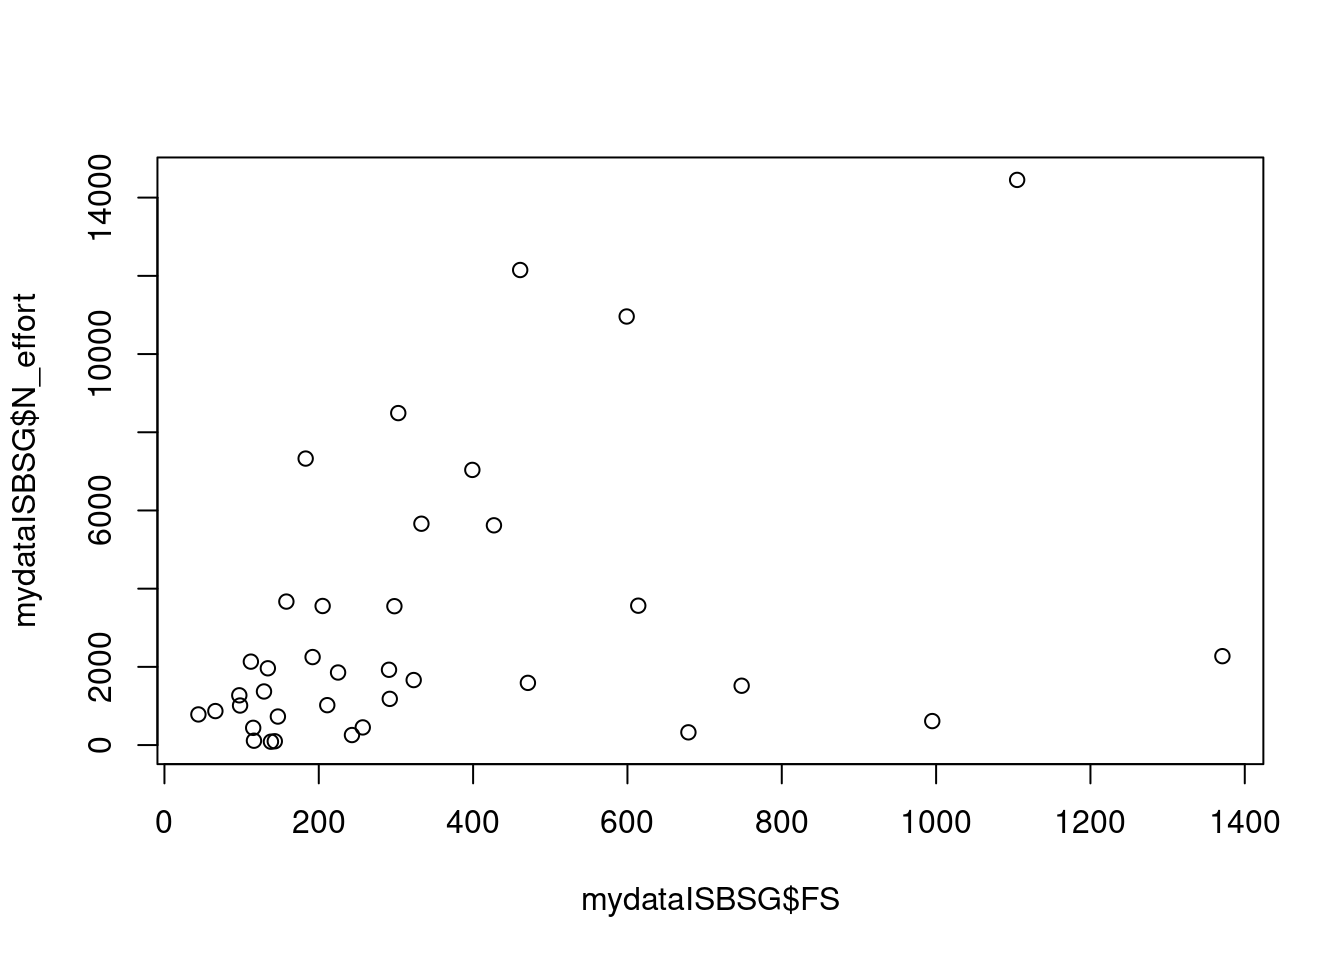
\includegraphics{DASE_files/figure-latex/plotExample-1.pdf}
\caption{\label{fig:plotExample}Simple plot}
\end{figure}

\begin{center}\rule{0.5\linewidth}{0.5pt}\end{center}

\hypertarget{control-flow-in-r}{%
\section{Control flow in R}\label{control-flow-in-r}}

R provides most common control flow structures found in most languages

\texttt{if}

\begin{Shaded}
\begin{Highlighting}[]
\NormalTok{x }\OtherTok{\textless{}{-}} \DecValTok{6}
\ControlFlowTok{if}\NormalTok{ (x }\SpecialCharTok{\textgreater{}=} \DecValTok{5}\NormalTok{) \{}
    \StringTok{"x is greater than or equals 5"}
\NormalTok{\} }\ControlFlowTok{else}\NormalTok{ \{}
    \StringTok{"x is smaller than 5"}
\NormalTok{\}}
\end{Highlighting}
\end{Shaded}

\begin{verbatim}
## [1] "x is greater than or equals 5"
\end{verbatim}

\texttt{ifelse}

\begin{Shaded}
\begin{Highlighting}[]
\FunctionTok{library}\NormalTok{(foreign)}
\NormalTok{kc1 }\OtherTok{\textless{}{-}} \FunctionTok{read.arff}\NormalTok{(}\StringTok{"datasets/defectPred/D1/KC1.arff"}\NormalTok{)}
\NormalTok{kc1}\SpecialCharTok{$}\NormalTok{Defective }\OtherTok{\textless{}{-}} \FunctionTok{ifelse}\NormalTok{(kc1}\SpecialCharTok{$}\NormalTok{Defective }\SpecialCharTok{==} \StringTok{"Y"}\NormalTok{, }\DecValTok{1}\NormalTok{, }\DecValTok{0}\NormalTok{)}
\FunctionTok{head}\NormalTok{(kc1, }\DecValTok{1}\NormalTok{)}
\end{Highlighting}
\end{Shaded}

\begin{verbatim}
##   LOC_BLANK BRANCH_COUNT LOC_CODE_AND_COMMENT LOC_COMMENTS
## 1         0            1                    0            0
##   CYCLOMATIC_COMPLEXITY DESIGN_COMPLEXITY ESSENTIAL_COMPLEXITY LOC_EXECUTABLE
## 1                     1                 1                    1              3
##   HALSTEAD_CONTENT HALSTEAD_DIFFICULTY HALSTEAD_EFFORT HALSTEAD_ERROR_EST
## 1            11.58                2.67           82.35               0.01
##   HALSTEAD_LENGTH HALSTEAD_LEVEL HALSTEAD_PROG_TIME HALSTEAD_VOLUME
## 1              11           0.38               4.57           30.88
##   NUM_OPERANDS NUM_OPERATORS NUM_UNIQUE_OPERANDS NUM_UNIQUE_OPERATORS LOC_TOTAL
## 1            4             7                   3                    4         5
##   Defective
## 1         0
\end{verbatim}

\texttt{for} loops

\begin{Shaded}
\begin{Highlighting}[]
\ControlFlowTok{for}\NormalTok{(x }\ControlFlowTok{in} \DecValTok{1}\SpecialCharTok{:}\DecValTok{5}\NormalTok{)\{}
  \FunctionTok{print}\NormalTok{(x)}
\NormalTok{\}}
\end{Highlighting}
\end{Shaded}

\hypertarget{built-in-datasets}{%
\section{Built-in Datasets}\label{built-in-datasets}}

R comes with some built-in datasets ready to use
\href{http://www.sthda.com/english/wiki/r-built-in-data-sets}{Description of datasets}
\url{http://www.sthda.com/english/wiki/r-built-in-data-sets}

\begin{Shaded}
\begin{Highlighting}[]
\FunctionTok{data}\NormalTok{()  }\CommentTok{\#list of datasets already available}
\end{Highlighting}
\end{Shaded}

Then, to load a dataset is as follows.

\begin{Shaded}
\begin{Highlighting}[]
\CommentTok{\# load the mtcars  Motor Trend Car Road Tests}
\FunctionTok{data}\NormalTok{(}\StringTok{"mtcars"}\NormalTok{)}
\end{Highlighting}
\end{Shaded}

And another example.

\begin{Shaded}
\begin{Highlighting}[]
\CommentTok{\# Monthly Airline Passenger Numbers 1949{-}1960}
\CommentTok{\# Time series object ts() convert a vector to a time series}
\FunctionTok{data}\NormalTok{(}\StringTok{"AirPassengers"}\NormalTok{)}
\FunctionTok{str}\NormalTok{(AirPassengers)}
\FunctionTok{plot}\NormalTok{(AirPassengers)}
\end{Highlighting}
\end{Shaded}

\hypertarget{other-tools-with-r}{%
\section{Other tools with R}\label{other-tools-with-r}}

\hypertarget{rattle}{%
\subsection{Rattle}\label{rattle}}

There is graphical interface, Rattle, that allow us to perform some data mining tasks with R \citep{Williams11}.

\begin{figure}
\centering
\includegraphics{./figures/rattle.png}
\caption{Rattle: GUI for Data mining with R}
\end{figure}

\hypertarget{jamovi}{%
\subsection{Jamovi}\label{jamovi}}

GUI for statistical analysis in R. It allow us to export the actual R code.
Its Website is: \url{https://www.jamovi.org/}

\begin{figure}
\centering
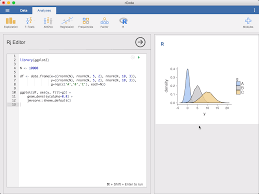
\includegraphics{./figures/jamovi.png}
\caption{Jamovi}
\end{figure}

\hypertarget{jasp}{%
\subsection{JASP}\label{jasp}}

There is another GUI for statistics, JASP, but it is not so easy at the moment to export the R code.
\url{https://jasp-stats.org/}

\hypertarget{part-introduction-to-data-mining}{%
\part{Introduction to Data Mining}\label{part-introduction-to-data-mining}}

We will deal with extracting information from data, either for estimation, defect prediction, planning, etc.

We will provide an overview of data analsyis using different techniques.

\hypertarget{what-is-data-mining-knowledge-discovery-in-databases-kdd}{%
\chapter{What is Data Mining / Knowledge Discovery in Databases (KDD)}\label{what-is-data-mining-knowledge-discovery-in-databases-kdd}}

The non-trivial process of identifying valid, novel, potentially useful, and ultimately understandable patterns in data \citep{FayyadPS1996}

\begin{figure}
\centering
\includegraphics{figures/Fayyad96kdd-process.png}
\caption{KDD Process}
\end{figure}

The Cross Industry Process for Data Mining (CRISP-DM) also provides a common and well-developed framework for delivering data mining projects identifying six steps \citep{shearer00crisp}:

\begin{enumerate}
\def\labelenumi{\arabic{enumi}.}
\tightlist
\item
  Problem Understanding
\item
  Data Understanding
\item
  Data Preparation
\item
  Modeling
\item
  Evaluation
\item
  Deployment
\end{enumerate}

\begin{figure}
\centering
\includegraphics{figures/CRISP-DM_Process_Diagram.png}
\caption{CRISP-DM (Wikipedia)}
\end{figure}

\hypertarget{the-aim-of-data-analysis-and-statistical-learning}{%
\section{The Aim of Data Analysis and Statistical Learning}\label{the-aim-of-data-analysis-and-statistical-learning}}

\begin{itemize}
\tightlist
\item
  The aim of any data analysis is to \textbf{understand the data}
\item
  and to build models for making predictions and estimating future events based on past data
\item
  and to make statistical inferences from our data.
\item
  We may want to test different hypothesis on the data
\item
  We want to generate conclusions about the population where our sample data comes from
\item
  Most probably we are interested in building a model for quality, time, defects or effort prediction
\end{itemize}

\includegraphics{figures/prediction.png}

\begin{itemize}
\tightlist
\item
  We want to find a function \(f()\), that given \(X1, X2, ...\) computes \(Y=f(X1, X2, ..., Xn)\)
\end{itemize}

\hypertarget{data-science}{%
\section{Data Science}\label{data-science}}

Data science (DS) is an inter-disciplinary field that uses scientific methods, processes, algorithms and systems to extract knowledge and insights from many structured and unstructured data. Data science is related to data mining, machine learning and big data.

We may say that the term DS embraces all terms related to data analysis that previously were under different disciplines.

\begin{figure}
\centering
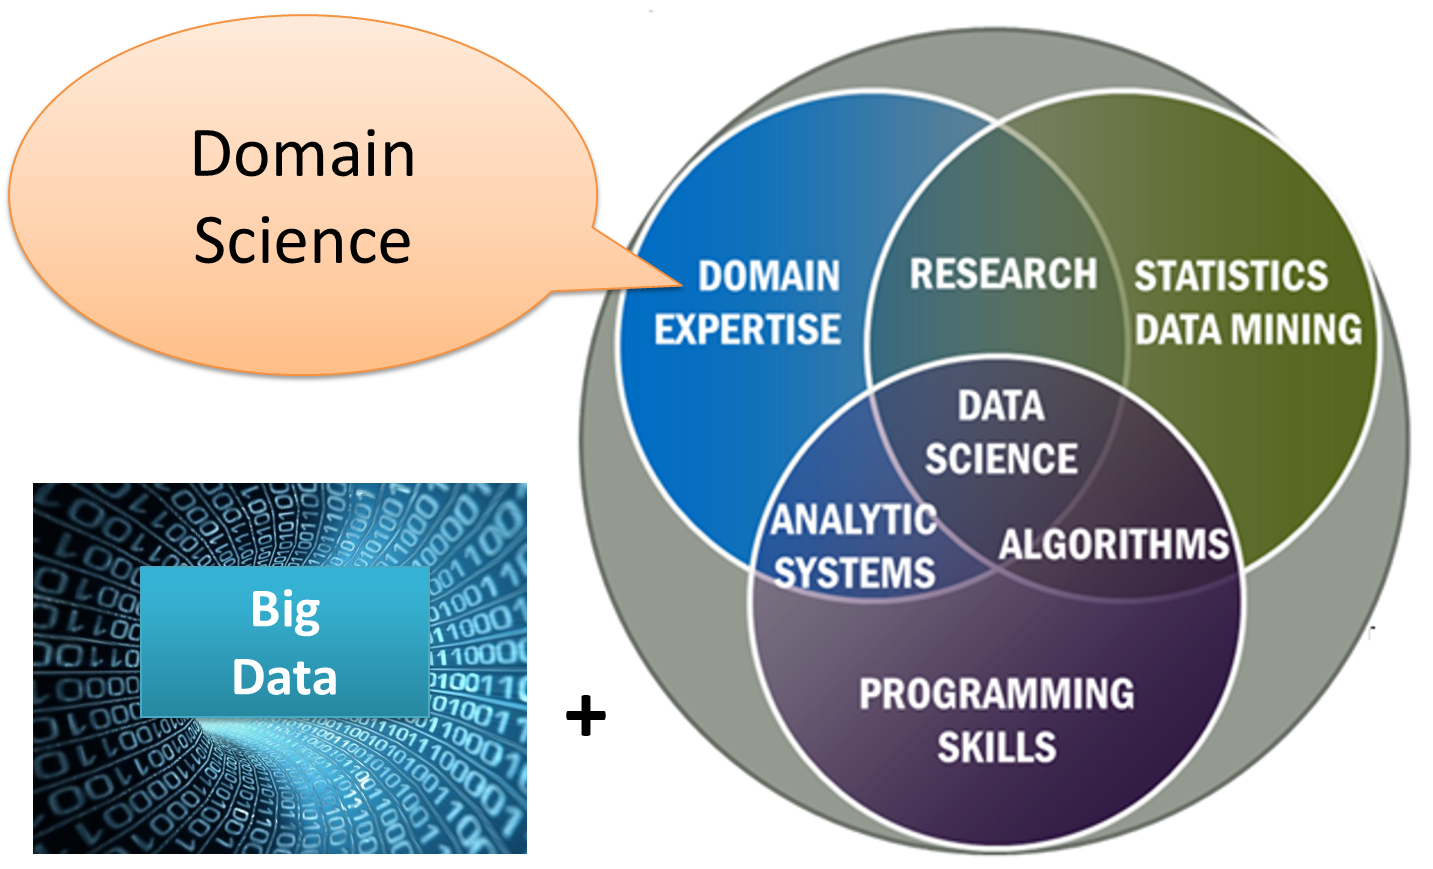
\includegraphics{figures/Data_science.png}
\caption{Wikipedia Data Science}
\end{figure}

\hypertarget{some-references}{%
\section{Some References}\label{some-references}}

\begin{itemize}
\tightlist
\item
  \href{https://cran.r-project.org/doc/manuals/r-release/R-intro.pdf}{W.N. Venables, D.M. Smith and the R Core Team, An Introduction to R}
\end{itemize}

Generic books about statistics:

\begin{itemize}
\item
  \href{https://cran.r-project.org/doc/contrib/Verzani-SimpleR.pdf}{John Verzani, \emph{simpleR - Using R for Introductory Statistics}}
\item
  \href{https://www.springer.com/gp/book/9780387790534}{Peter Dalgaard, \emph{Introductory Statistics with R}, 2nd Edt., Springer, 2008}
\item
  \href{http://www.springer.com/it/book/9781461471370}{Gareth James, Daniela Witten, Trevor Hastie, Robert Tibshirani, \emph{An Introduction to Statistical Learning with Applications in R}, Springer, 2013}
\item
  \href{https://www.routledge.com/products/9780415879682}{Geoff Cumming, \emph{Understanding the New Statistics: Effect Sizes, Confidence Intervals, and Meta-Analysis}, Routledge, New York, 2012}
\end{itemize}

\hypertarget{data-mining-and-data-science-with-r}{%
\section{Data Mining and Data Science with R}\label{data-mining-and-data-science-with-r}}

\begin{itemize}
\item
  \href{https://r4ds.had.co.nz/}{R for Data Science}
\item
  \href{https://www.manning.com/books/practical-data-science-with-r-second-edition}{Practical Data Science with R}
  *\href{https://www.jaredlander.com/r-for-everyone/}{R for Everyone: Advanced Analytics and Graphics}

  \begin{itemize}
  \item
    \href{http://www.springer.com/gp/book/9781441998897}{Graham Williams, \emph{Data Mining with Rattle and R: The Art of Excavating Data for Knowledge Discovery}, Springer 2011}

    Also the author maintains a Web site:
    \url{http://rattle.togaware.com/}
  \item
    \href{https://www.crcpress.com/Data-Mining-with-R-Learning-with-Case-Studies/Torgo/9781439810187}{Luis Torgo, \emph{Data Mining with R: Learning with Case Studies}, Chapman and Hall/CRC, 2010}
  \item
    \url{http://www.rdatamining.com/}
  \end{itemize}
\end{itemize}

\hypertarget{data-mining-with-weka}{%
\section{Data Mining with Weka}\label{data-mining-with-weka}}

Weka is another popular framework written in Java that can be used and extended with other languages and frameworks. The authors of Weka also have a popular book:

\begin{itemize}
\tightlist
\item
  Ian Witten, Eibe Frank, Mark Hall, Christopher J. Pal, Data Mining: Practical Machine Learning Tools and Techniques (4th Edt), Morgan Kaufmann, 2016, ISBN: 978-0128042915
\end{itemize}

\hypertarget{r-markdown}{%
\section{R Markdown}\label{r-markdown}}

Cheatsheet link for the markdown documents
\url{https://github.com/adam-p/markdown-here/wiki/Markdown-Cheatsheet}

This is an R Markdown document. Markdown is a simple formatting syntax for authoring HTML, PDF, and MS Word documents. For more details on using R Markdown see \url{http://rmarkdown.rstudio.com}.

When you click the \textbf{Knit} button a document will be generated that includes both content as well as the output of any embedded R code chunks within the document. You can embed an R code chunk like this:

\begin{Shaded}
\begin{Highlighting}[]
\FunctionTok{summary}\NormalTok{(cars)}
\end{Highlighting}
\end{Shaded}

\begin{verbatim}
##      speed           dist       
##  Min.   : 4.0   Min.   :  2.00  
##  1st Qu.:12.0   1st Qu.: 26.00  
##  Median :15.0   Median : 36.00  
##  Mean   :15.4   Mean   : 42.98  
##  3rd Qu.:19.0   3rd Qu.: 56.00  
##  Max.   :25.0   Max.   :120.00
\end{verbatim}

\hypertarget{including-plots}{%
\section{Including Plots}\label{including-plots}}

You can also embed plots, for example:

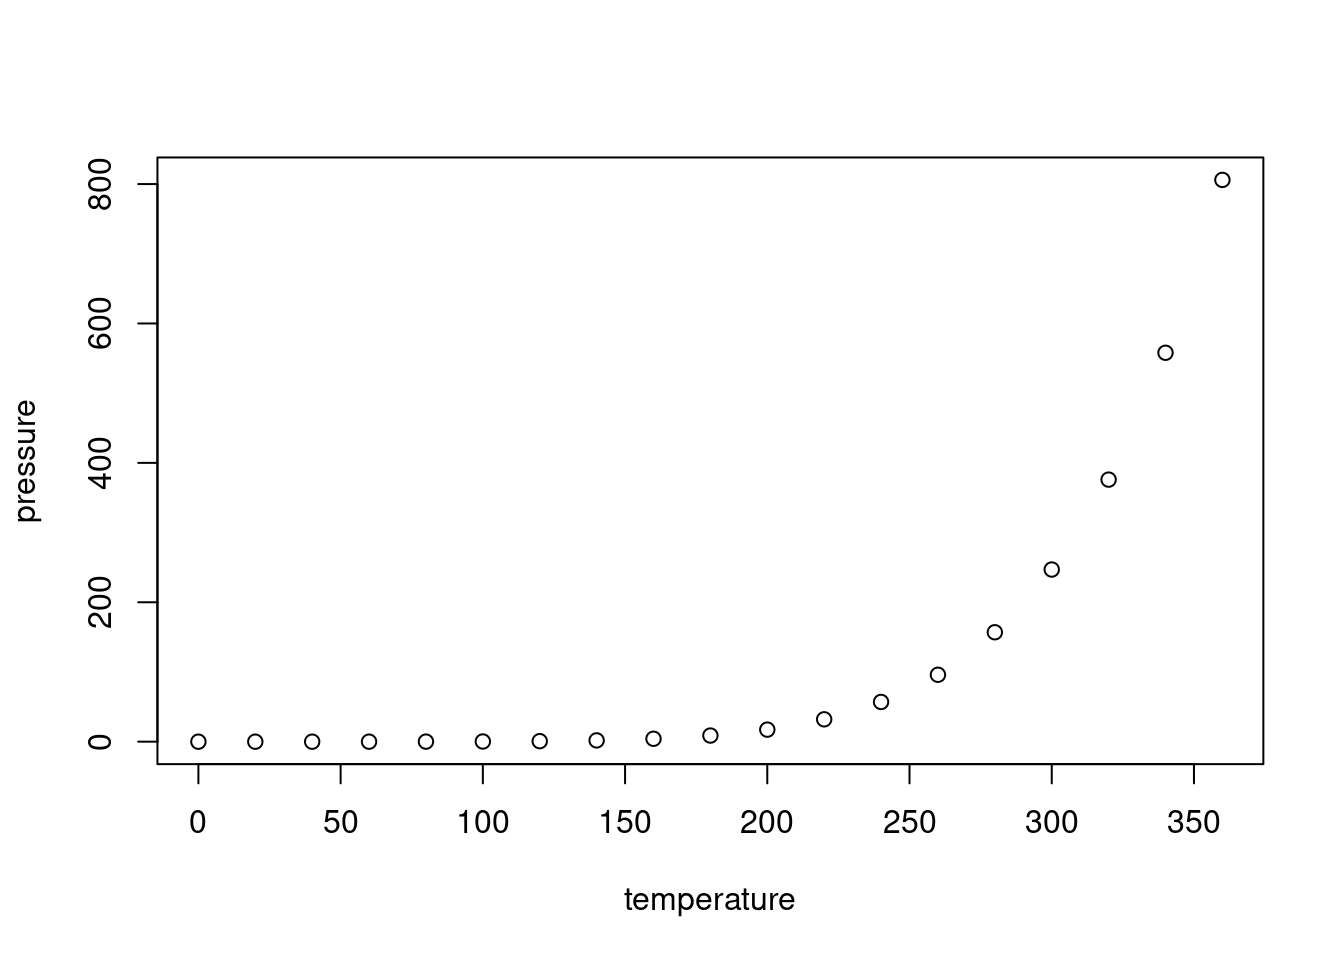
\includegraphics{DASE_files/figure-latex/pressure-1.pdf}

Note that the \texttt{echo\ =\ FALSE} parameter was added to the code chunk to prevent printing of the R code that generated the plot.

\hypertarget{references}{%
\section{References}\label{references}}

\url{https://github.com/adam-p/markdown-here/wiki/Markdown-Cheatsheet}
\url{https://rmarkdown.rstudio.com/lesson-15.html}

\begin{longtable}[]{@{}
  >{\raggedleft\arraybackslash}p{(\columnwidth - 0\tabcolsep) * \real{0.06}}@{}}
\toprule
\begin{minipage}[b]{\linewidth}\raggedleft
output: html\_document
pdf\_document: default
\end{minipage} \\
\midrule
\endhead
\#\# R and Python \\
R and Python can interact together via the \emph{reticulate} package. \\
The documentation for the \texttt{reticulate} package can be found here:
\url{https://rstudio.github.io/reticulate/} \\

\includegraphics{./figures/reticulated_python.png} \\
Instructions for configuring the system can be found at RStudio site: \url{https://support.rstudio.com/hc/en-us/articles/360023654474-Installing-and-Configuring-Python-with-RStudio}. \\
Or we can create our environment following - {[}R and Python -- a happy union with reticulate webinar{]}\url{https://www.youtube.com/watch?v=8WE-EU5k97Q\&t=27s} \\
\texttt{r\ install.packages("reticulate")} \\
Note that the \texttt{reticulate} package needs Python \textgreater= 2.7 and for \texttt{NumPy} requires NumPy \textgreater= 1.6. \\
\#\# Using Python with RMarkdown and RStudio \\
The R build-in dataset will be used later \\
\texttt{r\ library("reticulate")\ \#\ use\_virtualenv("myenv")\ data("mtcars")} \\
\texttt{python\ print("Hello\ Python!")} \\
\texttt{\#\#\ Hello\ Python!} \\
```python
datactrs = \{
`CHN': \{`COUNTRY': `China', `POP': 1\_398.72, `AREA': 9\_596.96,
`GDP': 12\_234.78, `CONT': `Asia'\},
`IND': \{`COUNTRY': `India', `POP': 1\_351.16, `AREA': 3\_287.26,
`GDP': 2\_575.67, `CONT': `Asia', `IND\_DAY': `1947-08-15'\},
`USA': \{`COUNTRY': `US', `POP': 329.74, `AREA': 9\_833.52,
`GDP': 19\_485.39, `CONT': `N.America',
`IND\_DAY': `1776-07-04'\},
`IDN': \{`COUNTRY': `Indonesia', `POP': 268.07, `AREA': 1\_910.93,
`GDP': 1\_015.54, `CONT': `Asia', `IND\_DAY': `1945-08-17'\},
`BRA': \{`COUNTRY': `Brazil', `POP': 210.32, `AREA': 8\_515.77,
`GDP': 2\_055.51, `CONT': `S.America', `IND\_DAY': `1822-09-07'\},
`PAK': \{`COUNTRY': `Pakistan', `POP': 205.71, `AREA': 881.91,
`GDP': 302.14, `CONT': `Asia', `IND\_DAY': `1947-08-14'\},
`NGA': \{`COUNTRY': `Nigeria', `POP': 200.96, `AREA': 923.77,
`GDP': 375.77, `CONT': `Africa', `IND\_DAY': `1960-10-01'\},
`BGD': \{`COUNTRY': `Bangladesh', `POP': 167.09, `AREA': 147.57,
`GDP': 245.63, `CONT': `Asia', `IND\_DAY': `1971-03-26'\},
`RUS': \{`COUNTRY': `Russia', `POP': 146.79, `AREA': 17\_098.25,
`GDP': 1\_530.75, `IND\_DAY': `1992-06-12'\},
`MEX': \{`COUNTRY': `Mexico', `POP': 126.58, `AREA': 1\_964.38,
`GDP': 1\_158.23, `CONT': `N.America', `IND\_DAY': `1810-09-16'\},
`JPN': \{`COUNTRY': `Japan', `POP': 126.22, `AREA': 377.97,
`GDP': 4\_872.42, `CONT': `Asia'\},
`DEU': \{`COUNTRY': `Germany', `POP': 83.02, `AREA': 357.11,
`GDP': 3\_693.20, `CONT': `Europe'\},
`FRA': \{`COUNTRY': `France', `POP': 67.02, `AREA': 640.68,
`GDP': 2\_582.49, `CONT': `Europe', `IND\_DAY': `1789-07-14'\},
`GBR': \{`COUNTRY': `UK', `POP': 66.44, `AREA': 242.50,
`GDP': 2\_631.23, `CONT': `Europe'\},
`ITA': \{`COUNTRY': `Italy', `POP': 60.36, `AREA': 301.34,
`GDP': 1\_943.84, `CONT': `Europe'\},
`ARG': \{`COUNTRY': `Argentina', `POP': 44.94, `AREA': 2\_780.40,
`GDP': 637.49, `CONT': `S.America', `IND\_DAY': `1816-07-09'\},
`DZA': \{`COUNTRY': `Algeria', `POP': 43.38, `AREA': 2\_381.74,
`GDP': 167.56, `CONT': `Africa', `IND\_DAY': `1962-07-05'\},
`CAN': \{`COUNTRY': `Canada', `POP': 37.59, `AREA': 9\_984.67,
`GDP': 1\_647.12, `CONT': `N.America', `IND\_DAY': `1867-07-01'\},
`AUS': \{`COUNTRY': `Australia', `POP': 25.47, `AREA': 7\_692.02,
`GDP': 1\_408.68, `CONT': `Oceania'\},
`KAZ': \{`COUNTRY': `Kazakhstan', `POP': 18.53, `AREA': 2\_724.90,
`GDP': 159.41, `CONT': `Asia', `IND\_DAY': `1991-12-16'\}
\} \\
columns = (`COUNTRY', `POP', `AREA', `GDP', `CONT', `IND\_DAY')
``` \\
```python
import pandas as pd
import seaborn as sns \#ubuntu \#sudo apt-get install -y python3-seaborn
import matplotlib.pyplot as plt \\
tips = sns.load\_dataset(``tips'')
mylist = {[}``youtube'', `linkedin', `1littlecoder'{]}
sns.scatterplot(x=tips{[}`total\_bill'{]}, y = tips{[}`tip'{]}, hue=tips{[}`day'{]})
plt.show()
``` \\
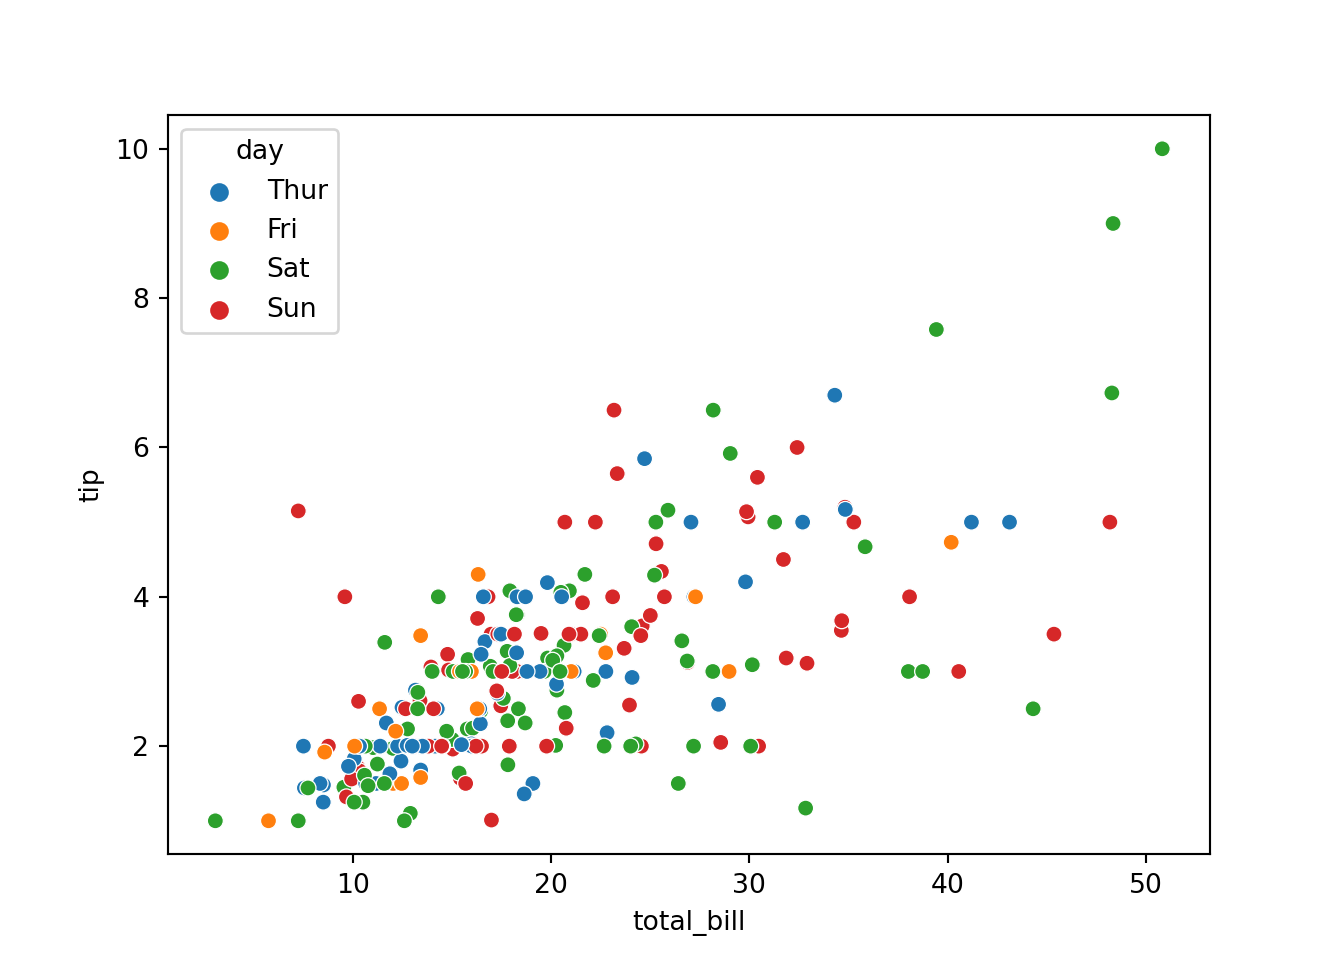
\includegraphics{DASE_files/figure-latex/impor_tips_fmri-1.pdf} \\
\texttt{python\ fmri\ =\ sns.load\_dataset("fmri")} \\
\texttt{r\ f1\ \textless{}-\ subset(py\$fmri,\ region\ ==\ "parietal")} \\
\texttt{python\ import\ matplotlib\ as\ mpl\ sns.lmplot("timepoint","signal",\ data=r.f1)} \\
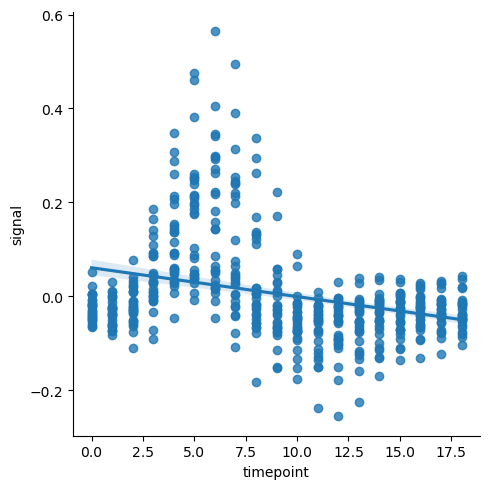
\includegraphics{DASE_files/figure-latex/accesing_r-1.pdf} \\
\texttt{python\ mpl.pyplot.show()} \\
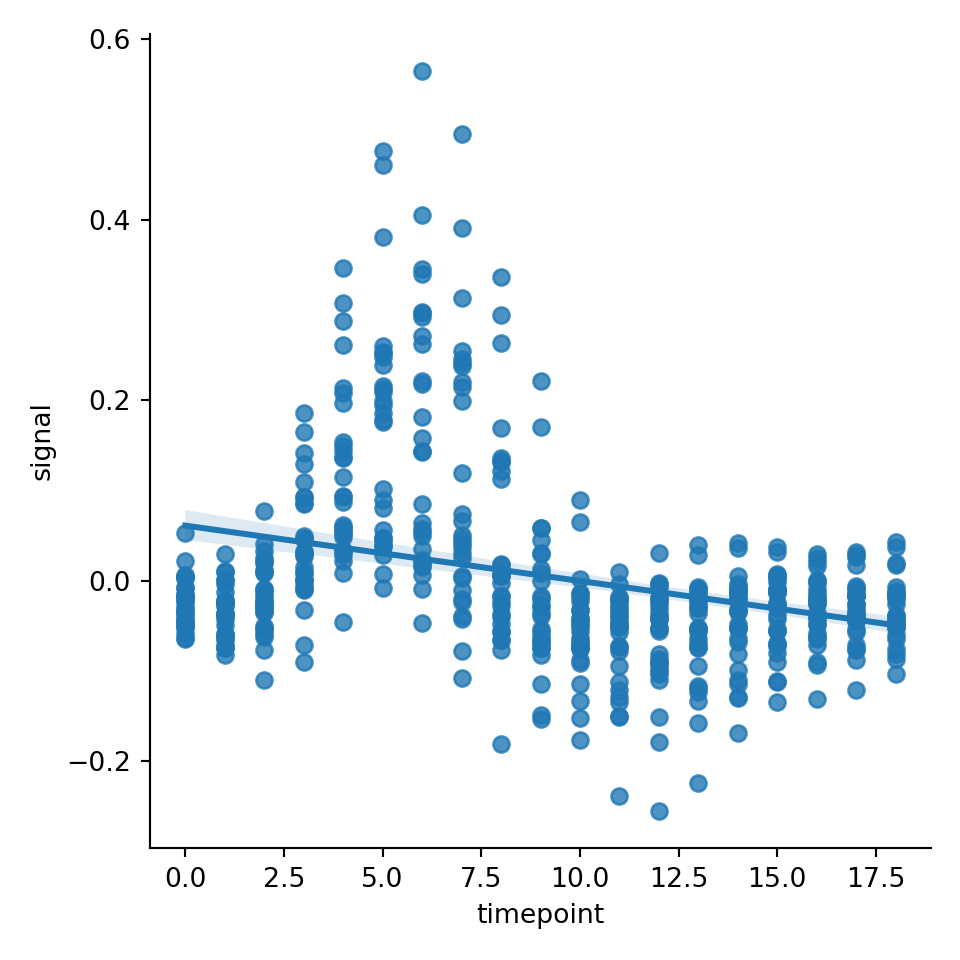
\includegraphics{DASE_files/figure-latex/accesing_r-2.pdf} \\
\texttt{python\ sns.lmplot("mpg",\ "cyl",\ data=r.mtcars)} \\
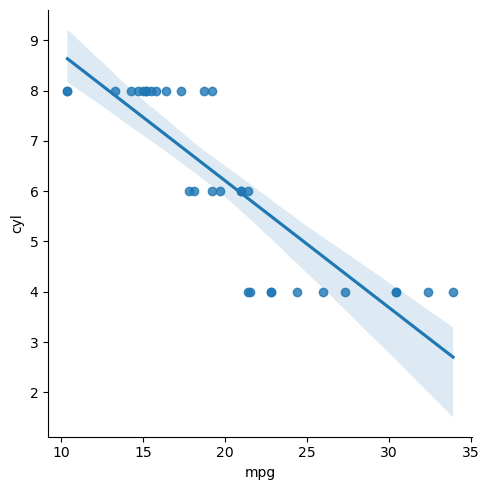
\includegraphics{DASE_files/figure-latex/accesing_r-3.pdf} \\
\texttt{python\ mpl.pyplot.show()} \\
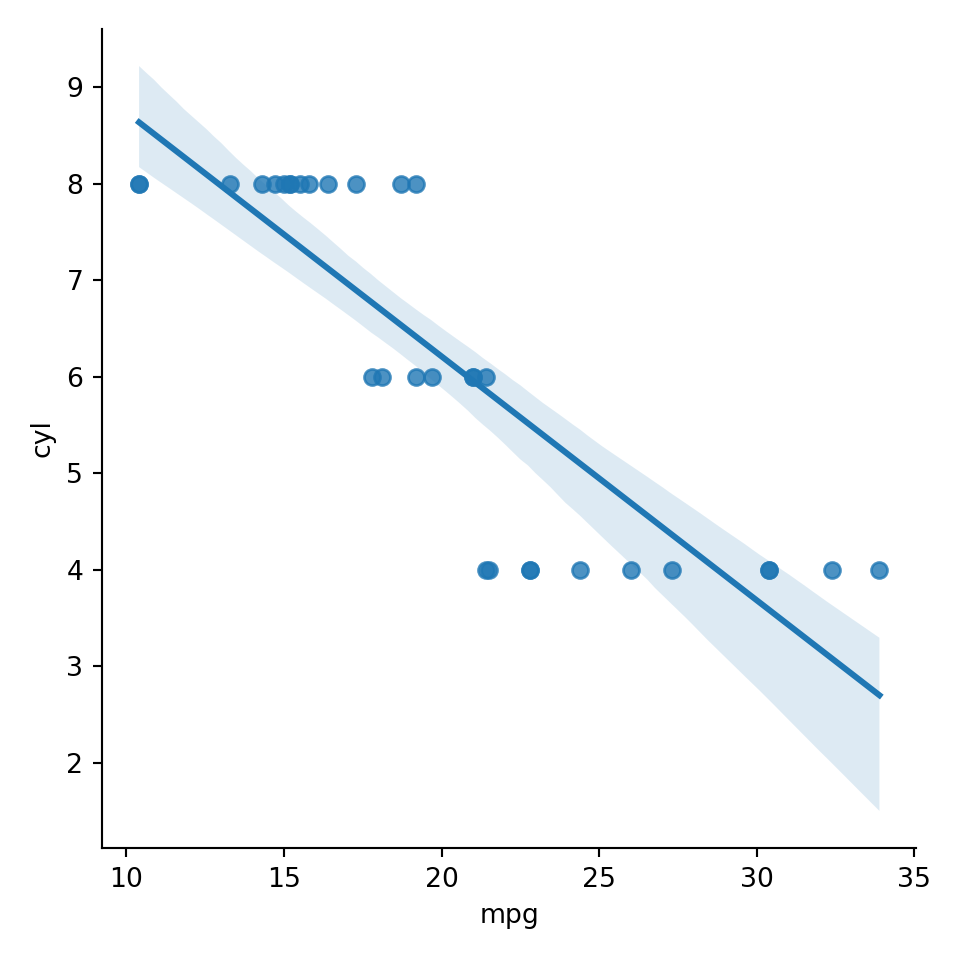
\includegraphics{DASE_files/figure-latex/accesing_r-4.pdf} \\
\texttt{python\ import\ pandas\ as\ pd\ df\ =\ pd.DataFrame(data=datactrs,\ index=columns).T\ df} \\
\texttt{\#\#\ \ \ \ \ \ \ \ \ COUNTRY\ \ \ \ \ \ POP\ \ \ \ \ \ AREA\ \ \ \ \ \ \ GDP\ \ \ \ \ \ \ CONT\ \ \ \ \ IND\_DAY\ \#\#\ CHN\ \ \ \ \ \ \ China\ \ 1398.72\ \ \ 9596.96\ \ 12234.78\ \ \ \ \ \ \ Asia\ \ \ \ \ \ \ \ \ NaN\ \#\#\ IND\ \ \ \ \ \ \ India\ \ 1351.16\ \ \ 3287.26\ \ \ 2575.67\ \ \ \ \ \ \ Asia\ \ 1947-08-15\ \#\#\ USA\ \ \ \ \ \ \ \ \ \ US\ \ \ 329.74\ \ \ 9833.52\ \ 19485.39\ \ N.America\ \ 1776-07-04\ \#\#\ IDN\ \ \ Indonesia\ \ \ 268.07\ \ \ 1910.93\ \ \ 1015.54\ \ \ \ \ \ \ Asia\ \ 1945-08-17\ \#\#\ BRA\ \ \ \ \ \ Brazil\ \ \ 210.32\ \ \ 8515.77\ \ \ 2055.51\ \ S.America\ \ 1822-09-07\ \#\#\ PAK\ \ \ \ Pakistan\ \ \ 205.71\ \ \ \ 881.91\ \ \ \ 302.14\ \ \ \ \ \ \ Asia\ \ 1947-08-14\ \#\#\ NGA\ \ \ \ \ Nigeria\ \ \ 200.96\ \ \ \ 923.77\ \ \ \ 375.77\ \ \ \ \ Africa\ \ 1960-10-01\ \#\#\ BGD\ \ Bangladesh\ \ \ 167.09\ \ \ \ 147.57\ \ \ \ 245.63\ \ \ \ \ \ \ Asia\ \ 1971-03-26\ \#\#\ RUS\ \ \ \ \ \ Russia\ \ \ 146.79\ \ 17098.25\ \ \ 1530.75\ \ \ \ \ \ \ \ NaN\ \ 1992-06-12\ \#\#\ MEX\ \ \ \ \ \ Mexico\ \ \ 126.58\ \ \ 1964.38\ \ \ 1158.23\ \ N.America\ \ 1810-09-16\ \#\#\ JPN\ \ \ \ \ \ \ Japan\ \ \ 126.22\ \ \ \ 377.97\ \ \ 4872.42\ \ \ \ \ \ \ Asia\ \ \ \ \ \ \ \ \ NaN\ \#\#\ DEU\ \ \ \ \ Germany\ \ \ \ 83.02\ \ \ \ 357.11\ \ \ \ 3693.2\ \ \ \ \ Europe\ \ \ \ \ \ \ \ \ NaN\ \#\#\ FRA\ \ \ \ \ \ France\ \ \ \ 67.02\ \ \ \ 640.68\ \ \ 2582.49\ \ \ \ \ Europe\ \ 1789-07-14\ \#\#\ GBR\ \ \ \ \ \ \ \ \ \ UK\ \ \ \ 66.44\ \ \ \ \ 242.5\ \ \ 2631.23\ \ \ \ \ Europe\ \ \ \ \ \ \ \ \ NaN\ \#\#\ ITA\ \ \ \ \ \ \ Italy\ \ \ \ 60.36\ \ \ \ 301.34\ \ \ 1943.84\ \ \ \ \ Europe\ \ \ \ \ \ \ \ \ NaN\ \#\#\ ARG\ \ \ Argentina\ \ \ \ 44.94\ \ \ \ 2780.4\ \ \ \ 637.49\ \ S.America\ \ 1816-07-09\ \#\#\ DZA\ \ \ \ \ Algeria\ \ \ \ 43.38\ \ \ 2381.74\ \ \ \ 167.56\ \ \ \ \ Africa\ \ 1962-07-05\ \#\#\ CAN\ \ \ \ \ \ Canada\ \ \ \ 37.59\ \ \ 9984.67\ \ \ 1647.12\ \ N.America\ \ 1867-07-01\ \#\#\ AUS\ \ \ Australia\ \ \ \ 25.47\ \ \ 7692.02\ \ \ 1408.68\ \ \ \ Oceania\ \ \ \ \ \ \ \ \ NaN\ \#\#\ KAZ\ \ Kazakhstan\ \ \ \ 18.53\ \ \ \ 2724.9\ \ \ \ 159.41\ \ \ \ \ \ \ Asia\ \ 1991-12-16} \\
\texttt{python\ df.to\_csv(\textquotesingle{}datasets/data\_countries.csv\textquotesingle{})}
We can read the dataset from python \\
\texttt{python\ df1\ =\ pd.read\_csv("datasets/other/data\_countries.csv",\ index\_col=0)} \\
Use R to read and write data from a package \\
\texttt{r\ library("nycflights13")\ write.csv(flights,\ "datasets/other/flights.csv")} \\
Use python to read the dataset and process the data \\
\texttt{python\ import\ pandas\ flights\ =\ pandas.read\_csv("datasets/other/flights.csv")\ flights\ =\ flights{[}flights{[}\textquotesingle{}dest\textquotesingle{}{]}\ =="ORD"{]}\ flights\ =\ flights{[}{[}\textquotesingle{}carrier\textquotesingle{},\ \textquotesingle{}dep\_delay\textquotesingle{},\ \textquotesingle{}arr\_delay\textquotesingle{}{]}{]}\ flights\ =\ flights.dropna()\ print(flights.head())} \\
\texttt{\#\#\ \ \ \ carrier\ \ dep\_delay\ \ arr\_delay\ \#\#\ 5\ \ \ \ \ \ \ UA\ \ \ \ \ \ \ -4.0\ \ \ \ \ \ \ 12.0\ \#\#\ 9\ \ \ \ \ \ \ AA\ \ \ \ \ \ \ -2.0\ \ \ \ \ \ \ \ 8.0\ \#\#\ 25\ \ \ \ \ \ MQ\ \ \ \ \ \ \ \ 8.0\ \ \ \ \ \ \ 32.0\ \#\#\ 38\ \ \ \ \ \ AA\ \ \ \ \ \ \ -1.0\ \ \ \ \ \ \ 14.0\ \#\#\ 57\ \ \ \ \ \ AA\ \ \ \ \ \ \ -4.0\ \ \ \ \ \ \ \ 4.0}
Use Python for plotting \\
\texttt{python\ import\ matplotlib.pyplot\ as\ plt\ import\ numpy\ as\ np\ t\ =\ np.arange(0.0,\ 2.0,\ 0.01)\ s\ =\ 1\ +\ np.sin(2*np.pi*t)\ plt.plot(t,s)\ plt.xlabel(\textquotesingle{}time\ (s)\textquotesingle{})\ plt.ylabel(\textquotesingle{}voltage\ (mV)\textquotesingle{})\ plt.grid(True)\ plt.savefig("test.png")\ plt.show()} \\
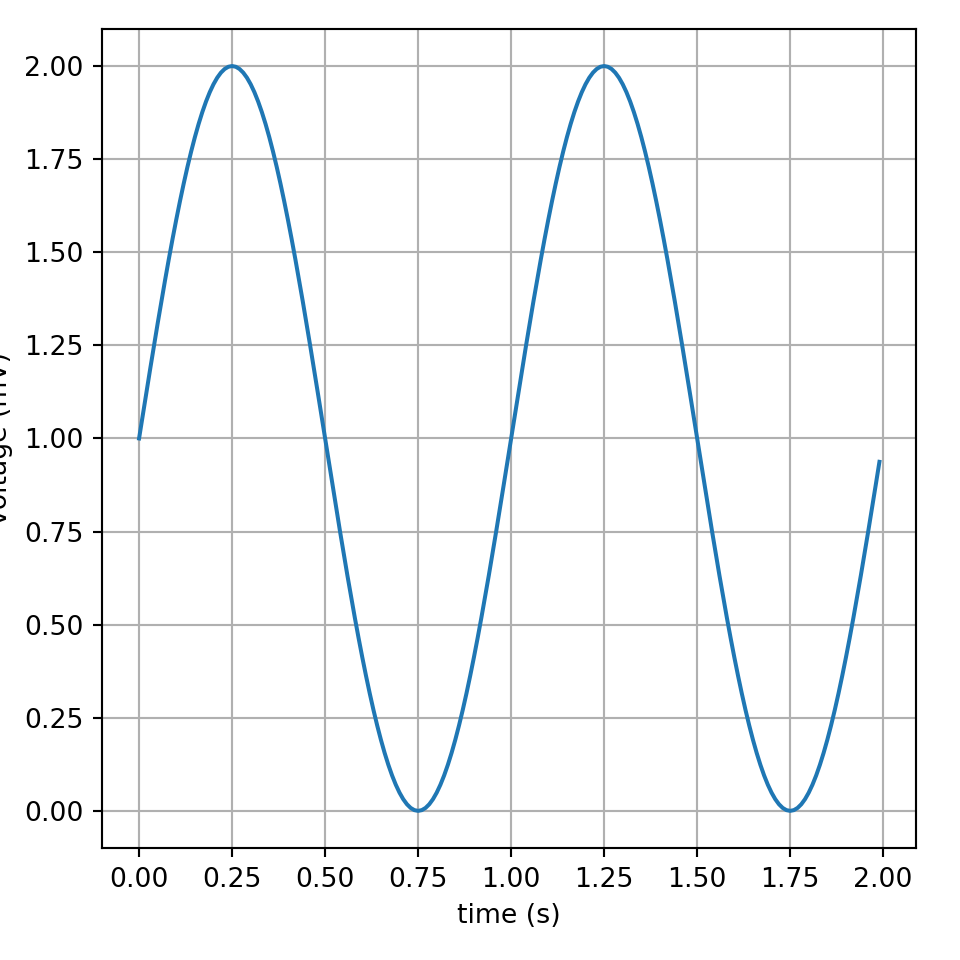
\includegraphics{DASE_files/figure-latex/matplotlib-1.pdf} \\
Use R for plotting Python objects:
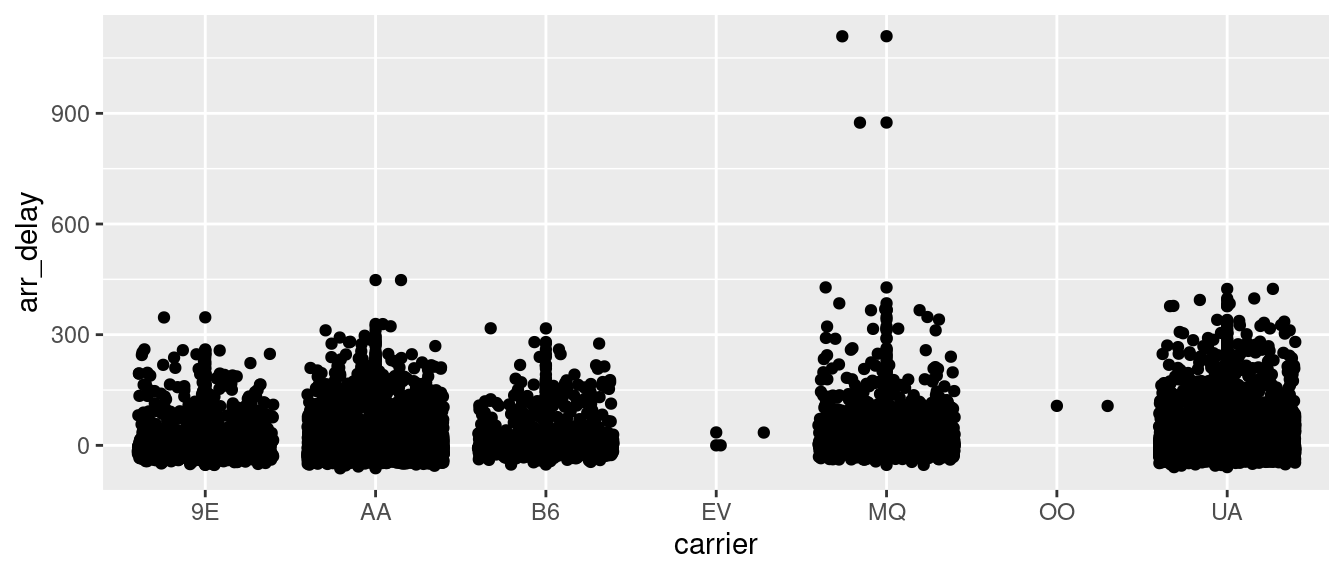
\includegraphics{DASE_files/figure-latex/unnamed-chunk-28-3.pdf} \\
Note that the \texttt{echo\ =\ FALSE} parameter was added to the code chunk to prevent printing of the R code that generated the plot. \\
\#\# References \\
- \href{https://info.rstudio.com/WN07MCXqS1A2NYS0040LW00}{https://rstudio.com/resources/webinars/rstudio-a-single-home-for-r-and-python/} \\
- \href{https://rstudio.github.io/reticulate/}{R interface to Python} \\
- \href{https://blog.rstudio.com/2020/07/28/practical-interoperability/}{3 Wild-Caught R and Python Applications} \\
- \href{https://www.r-bloggers.com/2021/01/rstudio-python-visual-markdown-editor-rstudio-latest-update/}{RStudio + Python, Visual Markdown Editor -- RStudio Latest Update} \\
- {[}Arrays in R and in Python{]}\url{https://rstudio.github.io/reticulate/articles/arrays.html} \\
- \url{https://www.r-bloggers.com/2021/02/pythons-pandas-vs-rs-dplyr-which-is-the-best-data-analysis-library/?utm_source=feedburner\&utm_medium=email\&utm_campaign=Feed\%3A+RBloggers+\%28R+bloggers\%29} \\
 \\
\# (PART) Data Sources and Metrics and Standards in Software Engineering Defect Prediction \{-\} \\
\# Data Sources in Software Engineering \\
We classify this trail in the following categories: \\
* \emph{Source code} can be studied to measure its properties, such as size or complexity. \\
* \emph{Source Code Management Systems} (SCM) make it possible to store all the changes that the different source code files undergo during the project. Also, SCM systems allow for work to be done in parallel by different developers over the same source code tree. Every change recorded in the system is accompanied with meta-information (author, date, reason for the change, etc) that can be used for research purposes. \\
* \emph{Issue or Bug tracking systems} (ITS). Bugs, defects and user requests are managed in ISTs, where users and developers can fill tickets with a description of a defect found, or a desired new functionality. All the changes to the ticket are recorded in the system, and most of the systems also record the comments and communications among all the users and developers implied in the task. \\
* \emph{Messages} between developers and users. In the case of free/open source software, the projects are open to the world, and the messages are archived in the form of mailing lists and social networks which can also be mined for research purposes. There are also some other open message systems, such as IRC or forums. \\
* \emph{Meta-data about the projects}. As well as the low level information of the software processes, we can also find meta-data about the software projects which can be useful for research. This meta-data may include intended-audience, programming language, domain of application, license (in the case of open source), etc. \\
\includegraphics{figures/artifactsMeta.png} \\
* \emph{Usage data}. There are statistics about software downloads, logs from servers, software reviews, etc. \\
Types of information stored in the repositories: \\
* Meta-information about the project itself and the
people that participated. \\
+ Low-level information \\
* Mailing Lists (ML) \\
* Bug Tracking Systems (BTS) or Project Tracker System (PTS) \\
* Software Configuration Management Systems (SCM) \\
+ Processed information. For example project management information about the effort estimation and cost of the project. \\
* Whether the repository is public or not \\
* Single project vs.~multiprojects. Whether the repository contains information of a single project with multiples versions or multiples projects and/or versions. \\
* Type of content, open source or industrial projects \\
* Format in which the information is stored and formats or technologies for accessing the information: \\
+ Text. It can be just plain text, CSV (Comma Separated Values) files, Attribute-Relation File Format
(ARFF) or its variants \\
+ Through databases. Downloading dumps of the database. \\
+ Remote access such as APIs of Web services or REST \\
\# Repositories \\
There is a number of open research repositories in Software Engineering. Among them: \\
+ Zenodo. It is becoming a popular site for publishing datasets associated with papers. It provides DOIs for referencing data and code:
\url{https://zenodo.org/} \\
+ Spinellis maintais a curated repository on Github:
\url{https://github.com/dspinellis/awesome-msr} \\
+ PROMISE (PRedictOr Models In Software Engineering). There is a conference with this name (\href{https://promiseconf.github.io/}{Promise Conference}) \\
Some popular datasets used as benchmarking in may paper can still be found on:
\url{http://promise.site.uottawa.ca/SERepository/datasets-page.html}
The is some well-known issues wit the NASA datasets and the source code is not available. \\
 \\
+ FLOSSMole \citep{HCC06}
\url{http://flossmole.org/} \\
+ FLOSSMetrics \citep{herraiz2009flossmetrics}:
\url{http://flossmetrics.org/} \\
+ Qualitas Corpus (QC) \citep{QualitasCorpus2010}:
\url{http://qualitascorpus.com/} \\
+ Sourcerer Project \citep{LBNRB09}:
\url{http://sourcerer.ics.uci.edu/} \\
+ Ultimate Debian Database (UDD) \citep{NZ10}
\url{http://udd.debian.org/} \\
+ SourceForge Research Data Archive (SRDA) \citep{VanAntwerpM2008}
\url{http://zerlot.cse.nd.edu/} \\
 \\
+ Software-artifact Infrastructure Repository (SIR)
{[}\url{http://sir.unl.edu}{]} \\
+ OpenHub:
\url{https://www.openhub.net/} \\
Not openly available (and mainly for effort estimation): \\
+ The International Software Benchmarking Standards Group (ISBSG)
\url{http://www.isbsg.org/} \\
 \\
Some papers and publications/theses that have been used in the literature: \\
+ Helix Data Set \citep{Vasa2010}:
\url{http://www.ict.swin.edu.au/research/projects/helix/} \\
+ Bug Prediction Dataset (BPD) \citep[\citet{ALR11}]{DAmb2010a}:
\url{http://bug.inf.usi.ch/} \\
+ Eclipse Bug Data (EBD) \citep[\citet{NZZH12}]{ZPZ07}:
\url{http://www.st.cs.uni-saarland.de/softevo/bug-data/eclipse/} \\
\# Open Tools/Dashboards to extract data \\
Process to extract data: \\
\includegraphics{./figures/process.png} \\
Within the open source community, several toolkits allow us to extract data that can be used to explore projects: \\
Metrics Grimoire
\url{http://metricsgrimoire.github.io/} \\
\includegraphics{figures/Grimoire.png} \\
SonarQube
\url{http://www.sonarqube.org/} \\
\includegraphics{figures/sonarQube.png} \\
CKJM (OO Metrics tool)
\url{http://gromit.iiar.pwr.wroc.pl/p_inf/ckjm/} \\
Collects a large number of object-oriented metrics from code. \\
\#\# Issues \\
There are problems such as different tools report different values for the same metric \citep{Lincke2008} \\
It is well-know that the NASA datasets have some problems: \\
+ \citep{Gray2011} The misuse of the NASA metrics data program data sets for automated software defect prediction \\
+ \citep{Shepperd2013} Data Quality: Some Comments on the NASA Software Defect Datasets \\
 \\
\#\# Effort Estimation Data in Software Engineering \\
It is worth highlighting the case of software effort estimation datasets with their peculiarities. First, most effort estimation datasets used in the literature are scattered through research papers with the exception of a few kept in the PROMISE repository. Mair et al \citeyearpar{MairSJ05} also have analysed available datasets in the field of cost estimation identifying 65 different datasets in 50 papers. \\
Second, their size is very small with the exception of ISBSG repository discussed previously which a small sample is available through PROMISE and the China dataset with 499 instances. \\
Third, some can be quite old in a context and time that is not applicable to current development environments. The authors noted that the oldest datasets (COCOMO, Desharnais, Kemerer and Albrecht and Gaffney) tend to be the most studied ones and a subset of the most relevant ones. Also, from the artificial intelligence or data mining point of view effort estimation has been mainly tackled with different types of regression techniques and more recently with techniques which are also typically considered under the umbrella of data mining techniques. However, as the number of examples per dataset is increasing, other machine learning techniques are also being studied (e.g.: Dejaeger et al \citeyearpar{Dejaeger_TSE12_EffEst} report on a comparison of several machine learning techniques to effort estimation with only 5 out the 9 used datasets publicly available). From the data mining point of view, the small number of instances hinders the application of machine learning techniques. \\
However, software effort and cost estimation still remain one of the main challenges in software engineering and have attracted a great deal of interest by many researchers \citeyearpar{Jorgensen07}. For example, there are continuous analyses of whether software development follows economies or diseconomies of scale (see \citep[\citet{Banker1994},\citet{Kitchenham2002}]{Dolado01_CostEst}). \\
Next Table \ref{tab:effEstimation} (following Mair et al \citeyearpar{MairSJ05} ) shows the most open cost/effort datasets available in the literature with their main reference. \\
Table: \label{tab:effEstimation} Effort Estimation Dataset from articles \\
\textbar{} Reference \textbar{} Instances \textbar{} Attributes \textbar{}
\textbar{} ----------------------------------\textbar{} ------------: \textbar------------:\textbar{}
\textbar Abran and Robillard \citeyearpar{Abran_TSE96_FP} \textbar{} 21 \textbar{} 31\textbar{}
\textbar Albrecht-Gaffney \citeyearpar{AlbrechtG83} \textbar{} 24 \textbar{} 7 \textbar{}
\textbar Bailey and Basili \citeyearpar{Bailey81} \textbar{} 18 \textbar{} 9 \textbar{}
\textbar Belady and Lehman \citeyearpar{Belady79} \textbar{} 33 \textbar{} \textbar{}
\textbar Boehm (aka COCOMO Dataset) \citeyearpar{Boehm81} \textbar{} 63 \textbar{} 43 \textbar{}
\textbar China dataset{[}\^{}1{]} \textbar{} 499 \textbar{} 18 \textbar{}
\textbar Desharnais \citeyearpar{Desharnais88} \textbar{} 61 \textbar{} 10 \textbar{}
\textbar Dolado \citeyearpar{Dolado97} \textbar{} 24 \textbar{} 7 \textbar{}
\textbar Hastings and Sajeev \citeyearpar{Hastings01} \textbar{} 8 \textbar{} 14 \textbar{}
\textbar Heiat and Heiat \citep{Heiat97} \textbar{} 35 \textbar{} 4 \textbar{}
\textbar Jeffery and Stathis \citeyearpar{Jeffery_ESE96} \textbar{} 17 \textbar{} 7 \textbar{}
\textbar Jorgensen \citeyearpar{Jorgensen04} \textbar{} 47 \textbar{} 4 \textbar{}
\textbar Jorgensen et al. \citeyearpar{Jorgensen2003} \textbar{} 20 \textbar{} 4 \textbar{}
\textbar Kemerer \citeyearpar{Kemerer87} \textbar{} 15 \textbar{} 5 \textbar{}
\textbar Kitchenham (Mermaid 2) \citeyearpar{Kitchenham2002} \textbar{} 30 \textbar{} 5 \textbar{}
\textbar Kitchenham et al.~(CSC) \citeyearpar{Kitchenham02_CSC} \textbar{} 145 \textbar{} 9 \textbar{}
\textbar Kitchenham and Taylor (ICL) \citeyearpar{Kitchenham85} \textbar{} 10 \textbar{} 6 \textbar{}
\textbar Kitchenham and Taylor (BT System X) \citeyearpar{Kitchenham85} \textbar{} 10 \textbar{} 3 \textbar{}
\textbar Kitchenham and Taylor (BT Software Houses) \citeyearpar{Kitchenham85} \textbar{} 12 \textbar{} 6 \textbar{}
\textbar Li et al.(USP05) \citeyearpar{LiRAR07}{[}\^{}2{]} \textbar{} 202 \textbar{} 16 \textbar{}
\textbar Mišić and Tevsić \citeyearpar{Misic19981} \textbar{} 6 \textbar{} 16 \textbar{}
\textbar Maxwell (Dev Effort) \citeyearpar{Maxwell02} \textbar{} 63 \textbar{} 32 \textbar{}
\textbar Maxwell (Maintenance Eff) \citeyearpar{Maxwell02} \textbar{} 67 \textbar{} 28 \textbar{}
\textbar Miyazaki et al. \citeyearpar{Miyazaki94} \textbar{} 47 \textbar{} 9 \textbar{}
\textbar Moser et al. \citeyearpar{Moser1999} \textbar{} 37 \textbar{} 4 \textbar{}
\textbar Shepperd and Cartwright \citep{Shepperd_TSE01} \textbar{} 39 \textbar{} 3 \textbar{}
\textbar Shepperd and Schofield (Telecom 1) \citeyearpar{Shepperd97_Analogy} \textbar{} 18 \textbar{} 5 \textbar{}
\textbar Schofield (real-time 1) \citeyearpar[\citet{Shepperd97_Analogy}]{Schofield98PhD} \textbar{} 21 \textbar{} 4 \textbar{}
\textbar Schofield (Mermaid) \citeyearpar{Schofield98PhD} \textbar{} 30 \textbar{} 18 \textbar{}
\textbar Schofield (Finnish) \citeyearpar{Schofield98PhD} \textbar{} 39 \textbar{} 30 \textbar{}
\textbar Schofield (Hughes) \citeyearpar{Schofield98PhD} \textbar{} 33 \textbar{} 14\textbar{}
\textbar Woodfield et al. \citeyearpar{Woodfield81} \textbar{} 63 \textbar{} 8 \textbar{} \\
{[}\^{}1{]}: Donated through PROMISE.
{[}\^{}2{]}: Only a subset of the data in the paper, the complete dataset is donated through PROMISE \\
 \\
\# (PART) Exploratory and Descriptive Data analysis \{-\} \\
\# Exploratory Data Analysis \\
\#\# Descriptive statistics \\
The first task to do with any dataset is to characterize it in terms of summary statistics and graphics. \\
Displaying information graphically will help us to identify the main characteristics of the data. To describe a distribution we often want to know where it is centered and and what the spread is (mean, median, quantiles) \\
\#\# Basic Plots \\
* \emph{Histogram} defines a sequence of breaks and then counts the number of observations in the bins formed by the breaks. \\
* \emph{Boxplot} used to summarize data succinctly, quickly displaying if the data is symmetric or has suspected outliers. \\
\includegraphics{./figures/boxplotexp.png} \\
* \emph{Q-Q plot} is used to determine if the data is close to being normally distributed. The quantiles of the standard normal distribution is represented by a straight line. The normality of the data can be evaluated by observing the extent in which the points appear on the line. When the data is normally distributed around the mean, then the mean and the median should be equal. Quantiles are cut points dividing the range of a probability distribution into continuous intervals with equal probabilities, or dividing the observations in a sample in the same way. \\
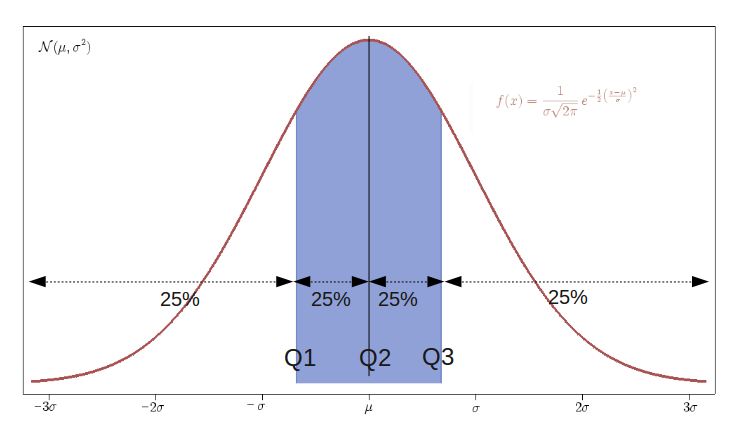
\includegraphics{./figures/Iqr_with_quantile.png} \\
* \emph{Scatterplot} provides a graphical view of the relationship between two sets of numbers: one numerical variable against another. \\
* \emph{Kernel Density} plot visualizes the underlying distribution of a variable. Kernel density estimation is a non-parametric method of estimating the probability density function of continuous random variable. It helps to identify the distribution of the variable. \\
* \emph{Violin plot} is a combination of a boxplot and a kernel density plot. \\
\#\# Normality \\
* A normal distribution is an arrangement of a data set in which most values cluster in the middle of the range
* A graphical representation of a normal distribution is sometimes called a \emph{bell curve} because of its shape.
* Many procedures in statistics are based on this property. \emph{Parametric} procedures require the normality property.
* In a normal distribution about 95\% of the probability lies within 2 Standard Deviations of the mean.
* Two examples: one population with mean 60 and the standard deviation of 1, and the other with mean 60 and \(sd=4\) (means shifted to 0) \\
\texttt{r\ \#\ Area\ within\ 2SD\ of\ the\ mean\ par(mfrow=c(1,2))\ plot(function(x)\ dnorm(x,\ mean\ =\ 0,\ sd\ =\ 1),\ xlim\ =\ c(-3,\ 3),\ main\ =\ "SD\ 1",\ xlab\ =\ "x",\ ylab\ =\ "",\ cex\ =\ 2)\ segments(-2,\ 0,\ -2,\ 0.4)\ segments(2,\ 0,\ 2,\ 0.4)\ \#\ Area\ within\ 4SD\ of\ the\ mean\ plot(function(x)\ dnorm(x,\ mean\ =\ 0,\ sd\ =\ 4),\ xlim\ =\ c(-12,\ 12),\ main\ =\ "SD\ 4",\ xlab\ =\ "x",\ ylab\ =\ "",\ cex\ =\ 2)\ segments(-8,\ 0,\ -8,\ 0.1)\ segments(8,\ 0,\ 8,\ 0.1)} \\
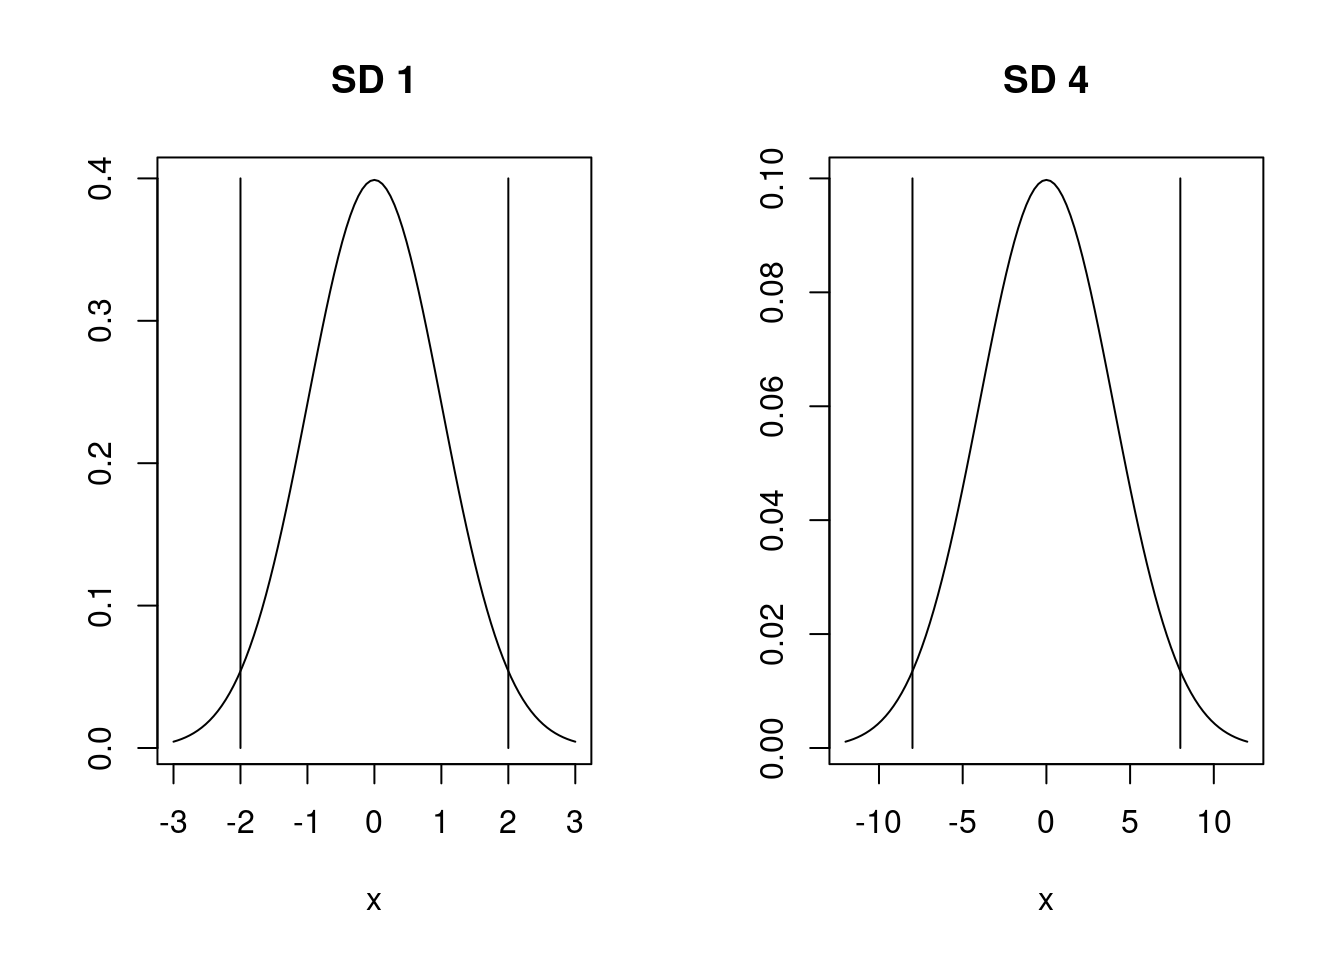
\includegraphics{DASE_files/figure-latex/SDPlotExample-1.pdf} \\
- if we sample from this population we get ``another population'': \\
```r
\#tidy uses the package formatR to format the code \\
sample.means \textless- rep(NA, 1000)
for (i in 1:1000) \{
sample.40 \textless- rnorm(40, mean = 60, sd = 4)
\#rnorm generates random numbers from normal distribution
sample.means{[}i{]} \textless- mean(sample.40)
\}
means40 \textless- mean(sample.means)
sd40 \textless- sd(sample.means)
means40
``` \\
\texttt{\#\#\ {[}1{]}\ 60.0144} \\
\texttt{r\ sd40} \\
\texttt{\#\#\ {[}1{]}\ 0.6592934} \\
- These sample means are another ``population''. The sampling distribution of the sample mean is normally distributed meaning that the ``mean of a representative sample provides an estimate of the unknown population mean''. This is shown in Figure \ref{fig:sampleMeansExample} \\
\texttt{r\ hist(sample.means)} \\
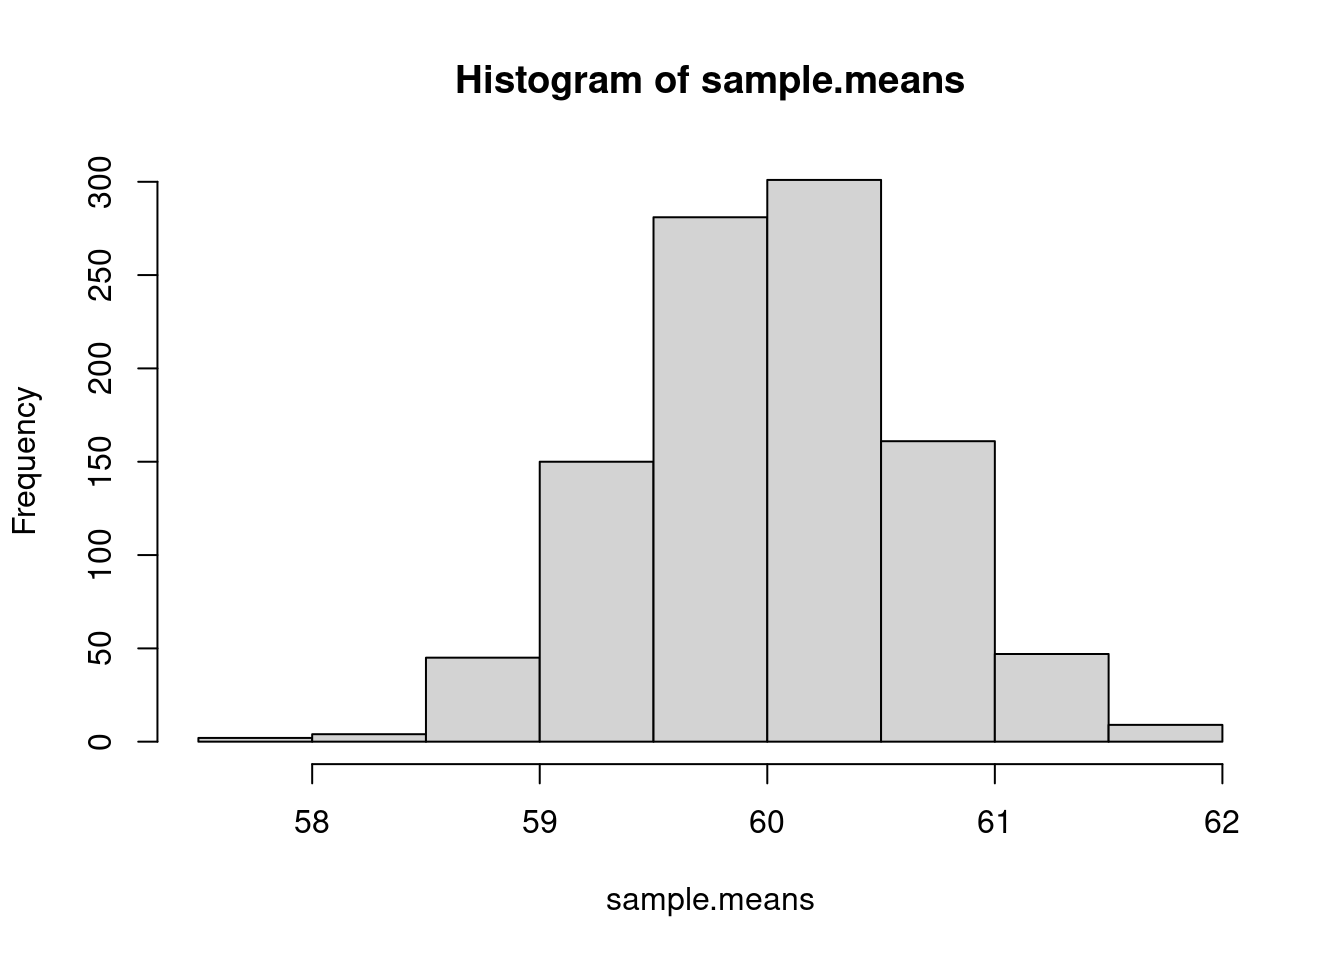
\includegraphics{DASE_files/figure-latex/sampleMeansExample-1.pdf} \\
\#\# Using a running Example to visualise the different plots \\
As a running example we do next: \\
1. Set the path to to the file \\
2. Read the \emph{Telecom1} dataset and print out the summary statistics with the command \texttt{summary} \\
\texttt{r\ options(digits=3)\ telecom1\ \textless{}-\ read.table("./datasets/effortEstimation/Telecom1.csv",\ sep=",",header=TRUE,\ stringsAsFactors=FALSE,\ dec\ =\ ".")\ \#read\ data\ summary(telecom1)} \\
\texttt{\#\#\ \ \ \ \ \ \ size\ \ \ \ \ \ \ \ \ \ \ effort\ \ \ \ \ \ \ \ EstTotal\ \#\#\ \ Min.\ \ \ :\ \ 3.0\ \ \ Min.\ \ \ :\ \ 24\ \ \ Min.\ \ \ :\ 30\ \#\#\ \ 1st\ Qu.:\ 37.2\ \ \ 1st\ Qu.:\ 119\ \ \ 1st\ Qu.:142\ \#\#\ \ Median\ :\ 68.5\ \ \ Median\ :\ 222\ \ \ Median\ :289\ \#\#\ \ Mean\ \ \ :100.3\ \ \ Mean\ \ \ :\ 284\ \ \ Mean\ \ \ :320\ \#\#\ \ 3rd\ Qu.:164.0\ \ \ 3rd\ Qu.:\ 352\ \ \ 3rd\ Qu.:472\ \#\#\ \ Max.\ \ \ :284.0\ \ \ Max.\ \ \ :1116\ \ \ Max.\ \ \ :777} \\
* We see that this dataset has three variables (or parameters) and few data points (18)
+ \emph{size}: the independent variable
+ \emph{effort}: the dependent variable
+ \emph{EstTotal}: the estimates coming from an estimation method
* Basic Plots \\
```r
par(mfrow=c(1,2)) \#n figures per row
size\_telecom1 \textless- telecom1\(size effort_telecom1 <- telecom1\)effort \\
hist(size\_telecom1, col=``blue'', xlab=`size', ylab = `Probability', main = `Histogram of project Size')
lines(density(size\_telecom1, na.rm = T, from = 0, to = max(size\_telecom1)))
plot(density(size\_telecom1))
``` \\
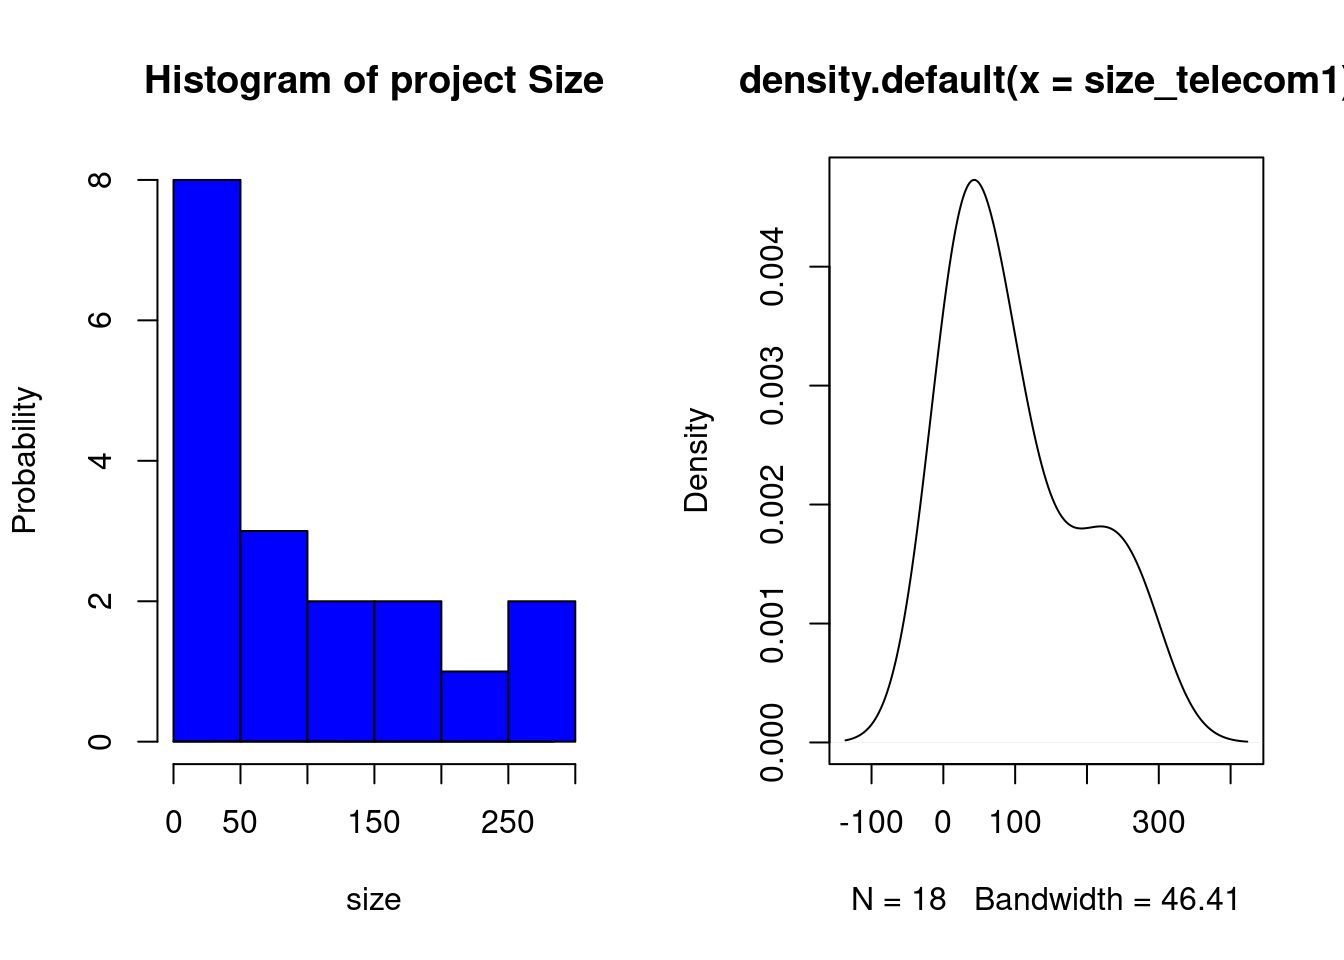
\includegraphics{DASE_files/figure-latex/unnamed-chunk-30-1.pdf} \\
\texttt{r\ hist(effort\_telecom1,\ col="blue")\ plot(density(effort\_telecom1))} \\
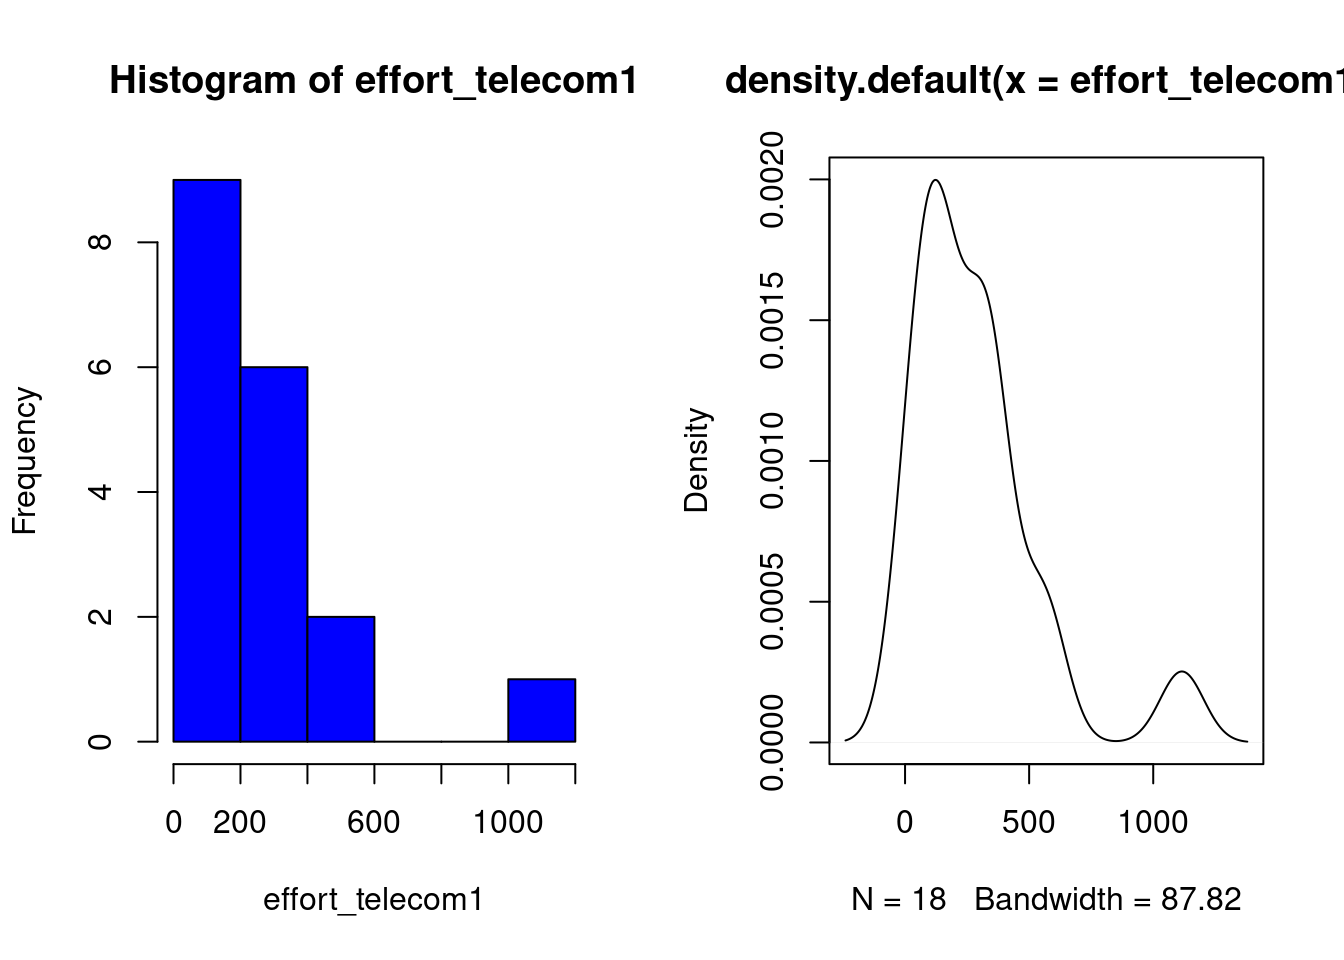
\includegraphics{DASE_files/figure-latex/unnamed-chunk-30-2.pdf} \\
\texttt{r\ boxplot(size\_telecom1)\ boxplot(effort\_telecom1)} \\
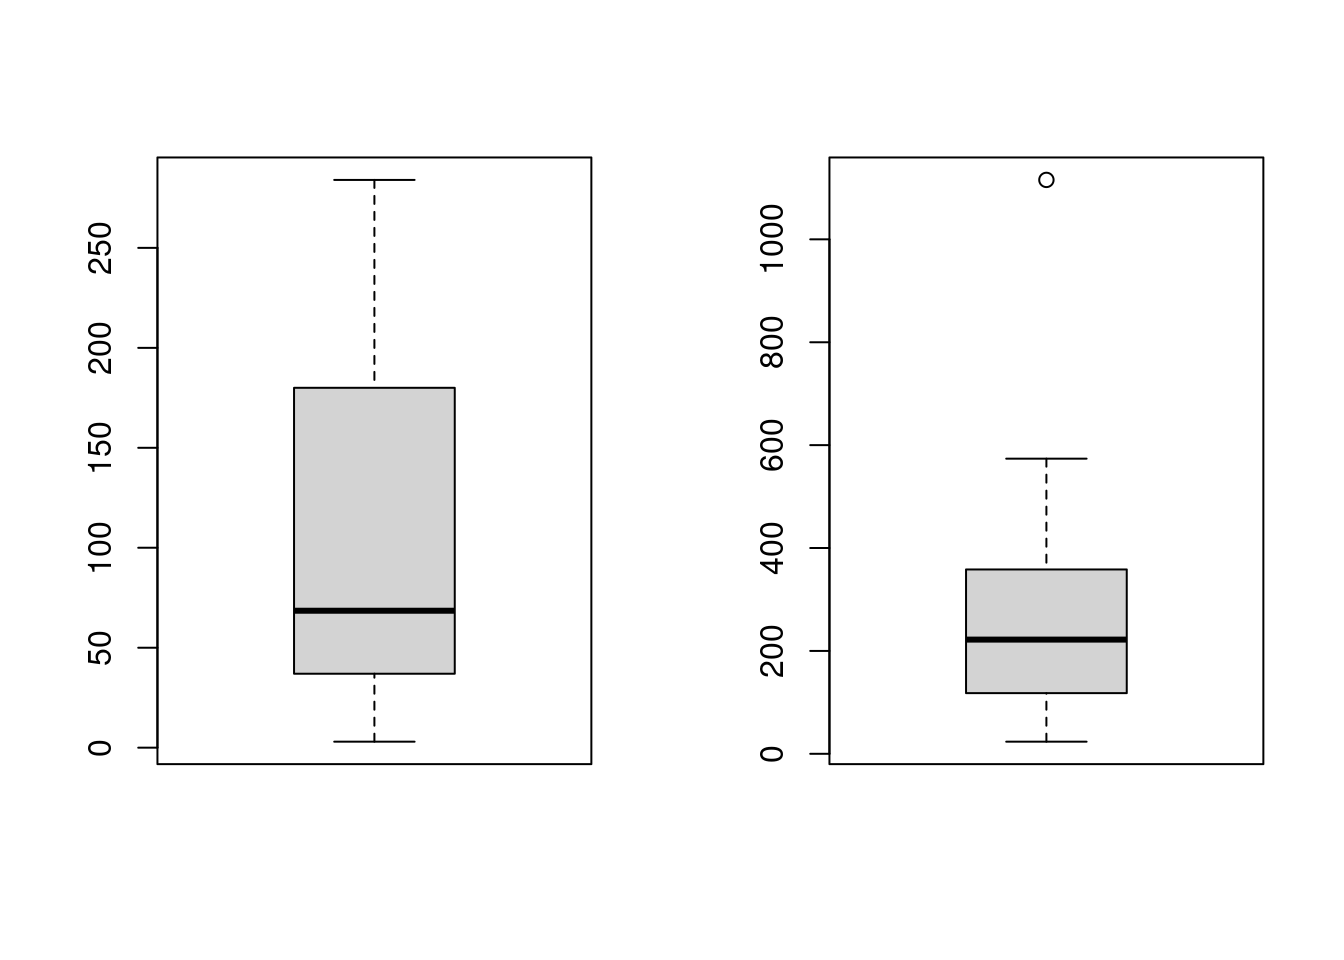
\includegraphics{DASE_files/figure-latex/unnamed-chunk-30-3.pdf} \\
\texttt{r\ \#\ violin\ plots\ for\ those\ two\ variables\ library(vioplot)\ vioplot(size\_telecom1,\ names\ =\ \textquotesingle{}\textquotesingle{})\ title("Violin\ Plot\ of\ Project\ Size")\ vioplot(effort\_telecom1,\ names\ =\ \textquotesingle{}\textquotesingle{})\ title("Violin\ Plot\ of\ Project\ Effort")} \\
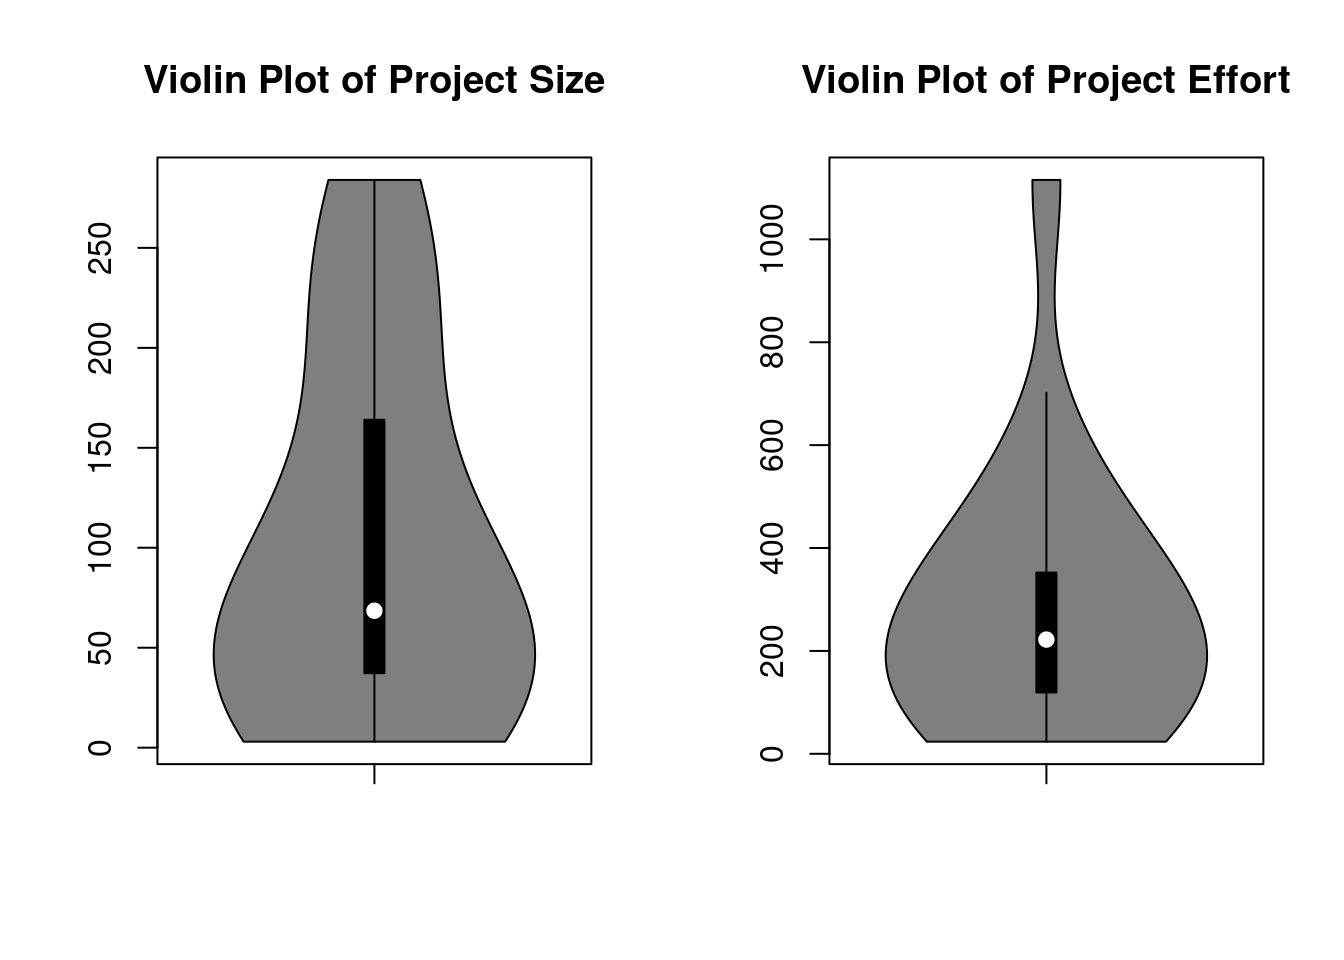
\includegraphics{DASE_files/figure-latex/unnamed-chunk-30-4.pdf} \\
\texttt{r\ par(mfrow=c(1,1))\ qqnorm(size\_telecom1,\ main="Q-Q\ Plot\ of\ \textquotesingle{}size\textquotesingle{}")\ qqline(size\_telecom1,\ col=2,\ lwd=2,\ lty=2)\ \#draws\ a\ line\ through\ the\ first\ and\ third\ quartiles} \\
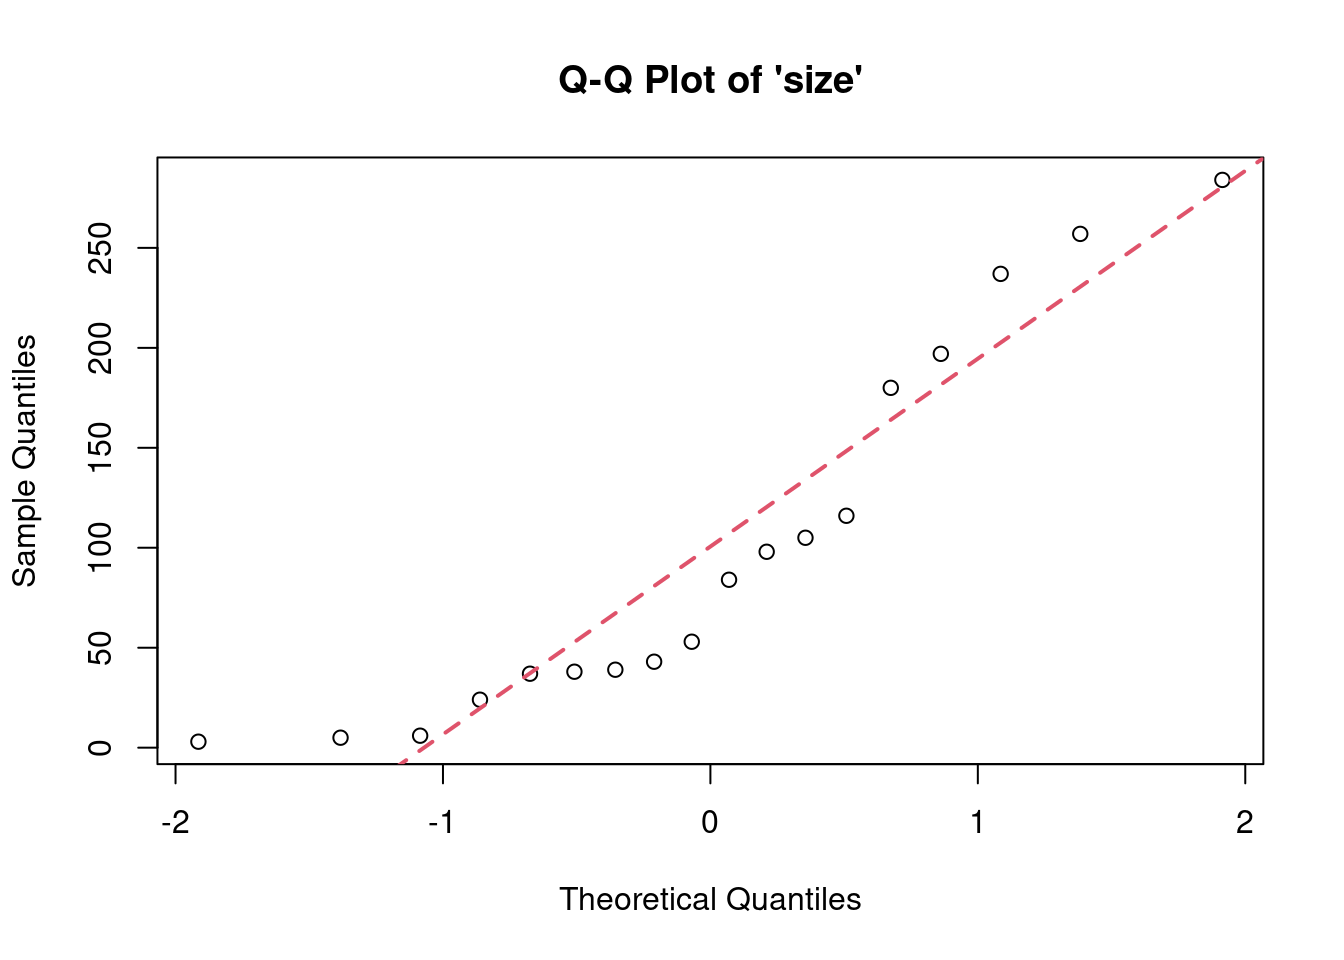
\includegraphics{DASE_files/figure-latex/unnamed-chunk-30-5.pdf} \\
\texttt{r\ qqnorm(effort\_telecom1,\ \ main="Q-Q\ Plot\ of\ \textquotesingle{}effort\textquotesingle{}")\ qqline(effort\_telecom1)} \\
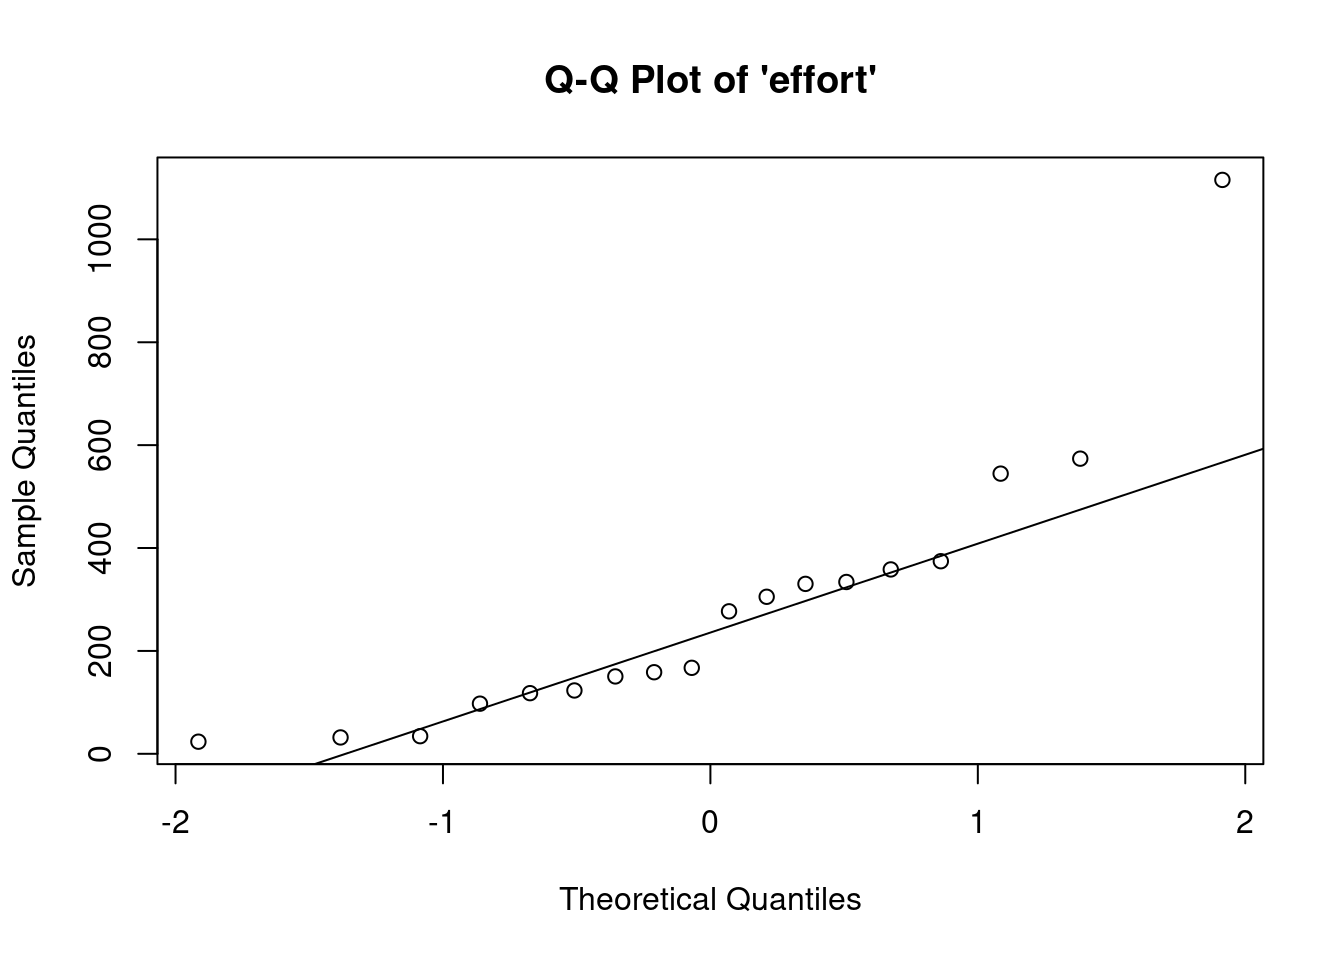
\includegraphics{DASE_files/figure-latex/unnamed-chunk-30-6.pdf} \\
* We can observe the non-normality of the data. \\
* We may look the possible relationship between size and effort with a scatter plot \\
\texttt{r\ plot(size\_telecom1,\ effort\_telecom1)} \\
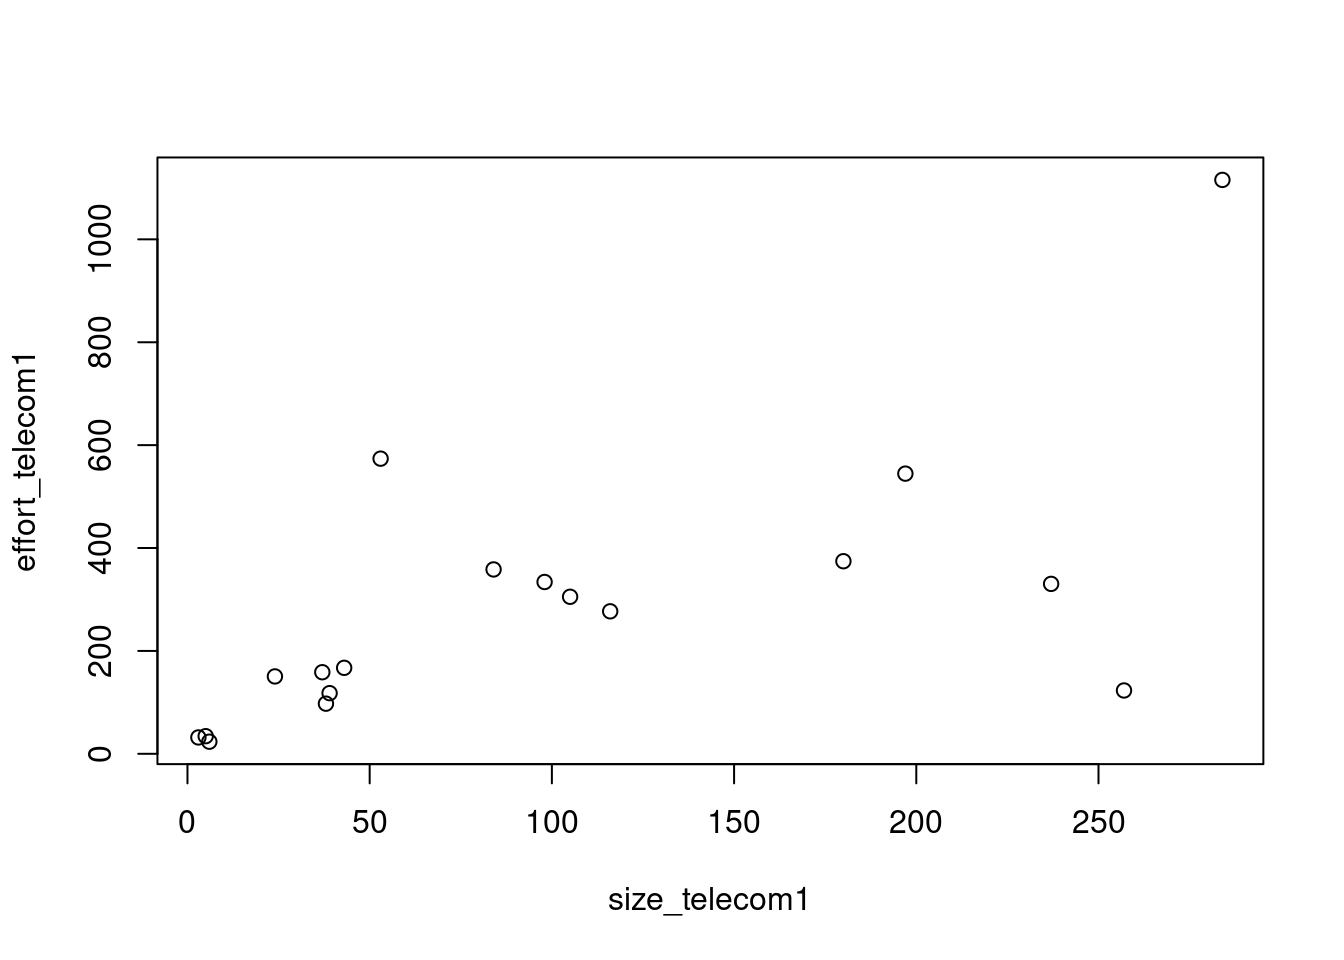
\includegraphics{DASE_files/figure-latex/scatterplotExample-1.pdf} \\
\#\#\# Example with the China dataset \\
\texttt{r\ library(foreign)\ china\ \textless{}-\ read.arff("./datasets/effortEstimation/china.arff")\ china\_size\ \textless{}-\ china\$AFP\ summary(china\_size)} \\
\texttt{\#\#\ \ \ \ Min.\ 1st\ Qu.\ \ Median\ \ \ \ Mean\ 3rd\ Qu.\ \ \ \ Max.\ \#\#\ \ \ \ \ \ \ 9\ \ \ \ \ 100\ \ \ \ \ 215\ \ \ \ \ 487\ \ \ \ \ 438\ \ \ 17518} \\
\texttt{r\ china\_effort\ \textless{}-\ china\$Effort\ summary(china\_effort)} \\
\texttt{\#\#\ \ \ \ Min.\ 1st\ Qu.\ \ Median\ \ \ \ Mean\ 3rd\ Qu.\ \ \ \ Max.\ \#\#\ \ \ \ \ \ 26\ \ \ \ \ 704\ \ \ \ 1829\ \ \ \ 3921\ \ \ \ 3826\ \ \ 54620} \\
\texttt{r\ par(mfrow=c(1,2))\ hist(china\_size,\ col="blue",\ xlab="Adjusted\ Function\ Points",\ main="Distribution\ of\ AFP")\ hist(china\_effort,\ col="blue",xlab="Effort",\ main="Distribution\ of\ Effort")} \\
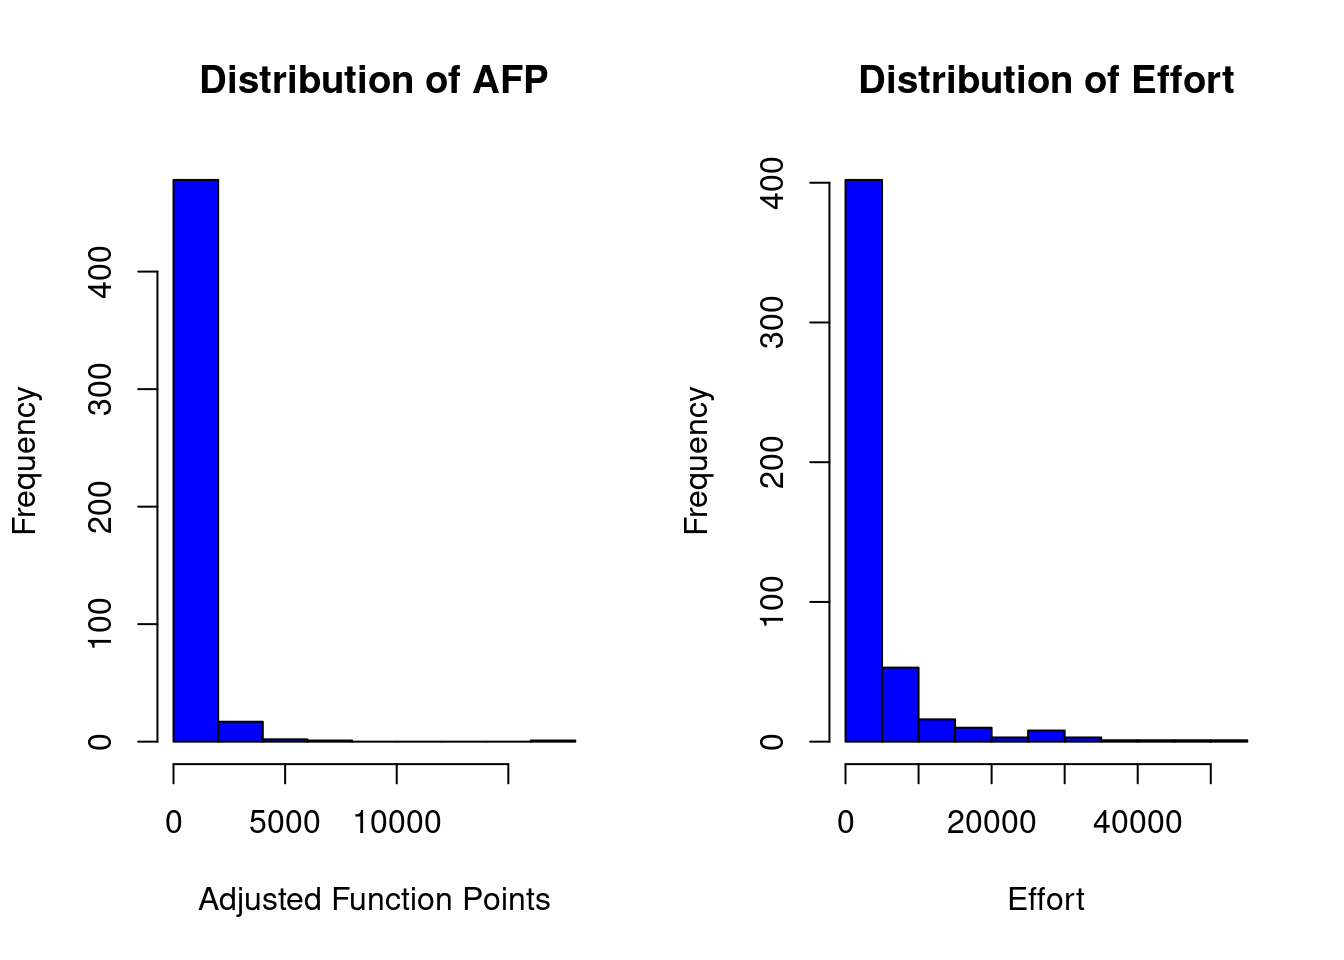
\includegraphics{DASE_files/figure-latex/unnamed-chunk-31-1.pdf} \\
\texttt{r\ boxplot(china\_size)\ boxplot(china\_effort)} \\
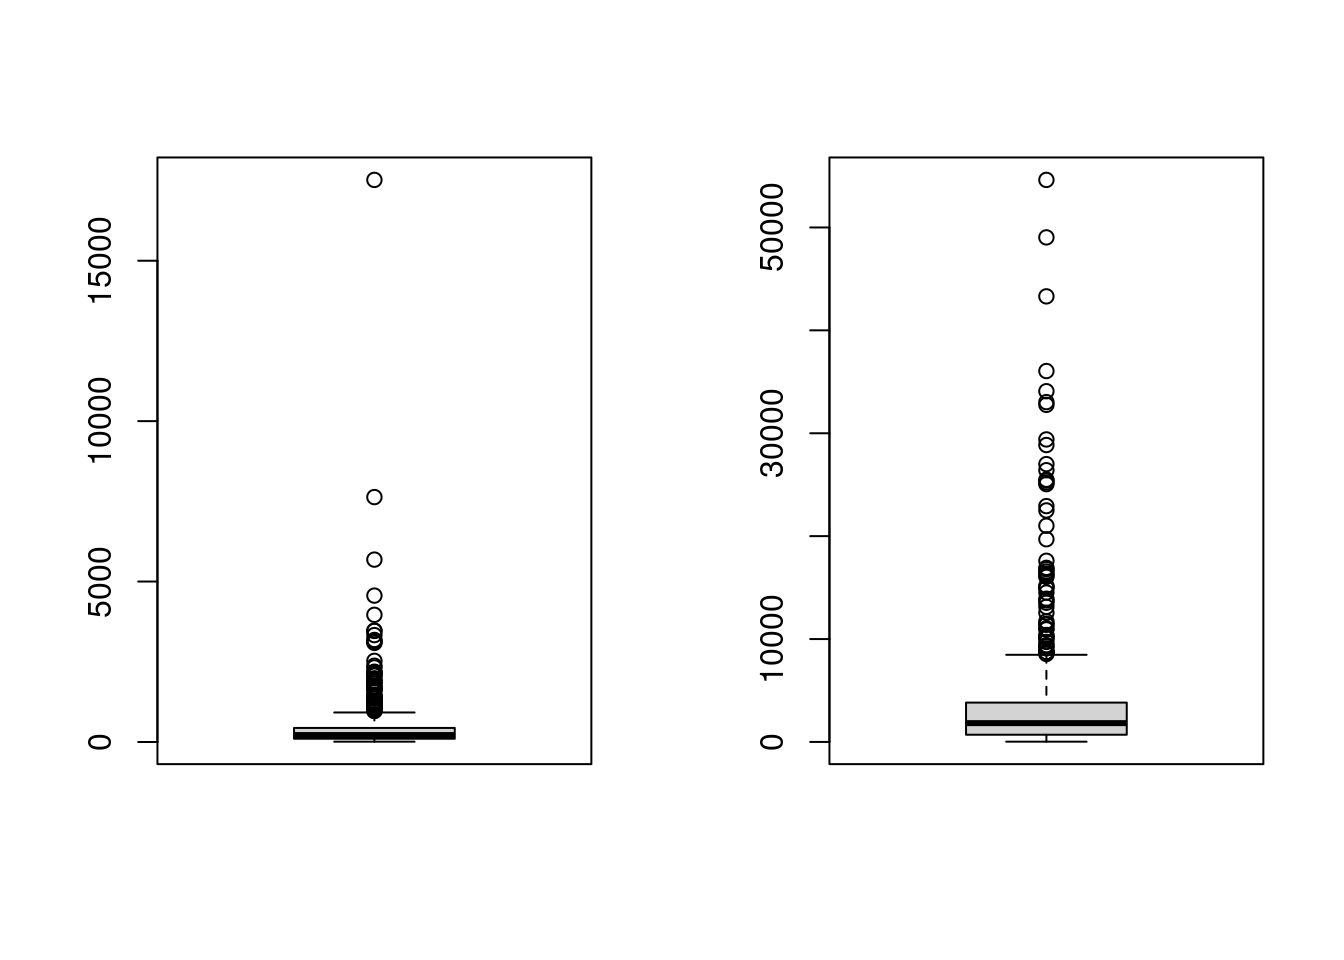
\includegraphics{DASE_files/figure-latex/unnamed-chunk-31-2.pdf} \\
\texttt{r\ qqnorm(china\_size)\ qqline(china\_size)\ qqnorm(china\_effort)\ qqline(china\_effort)} \\
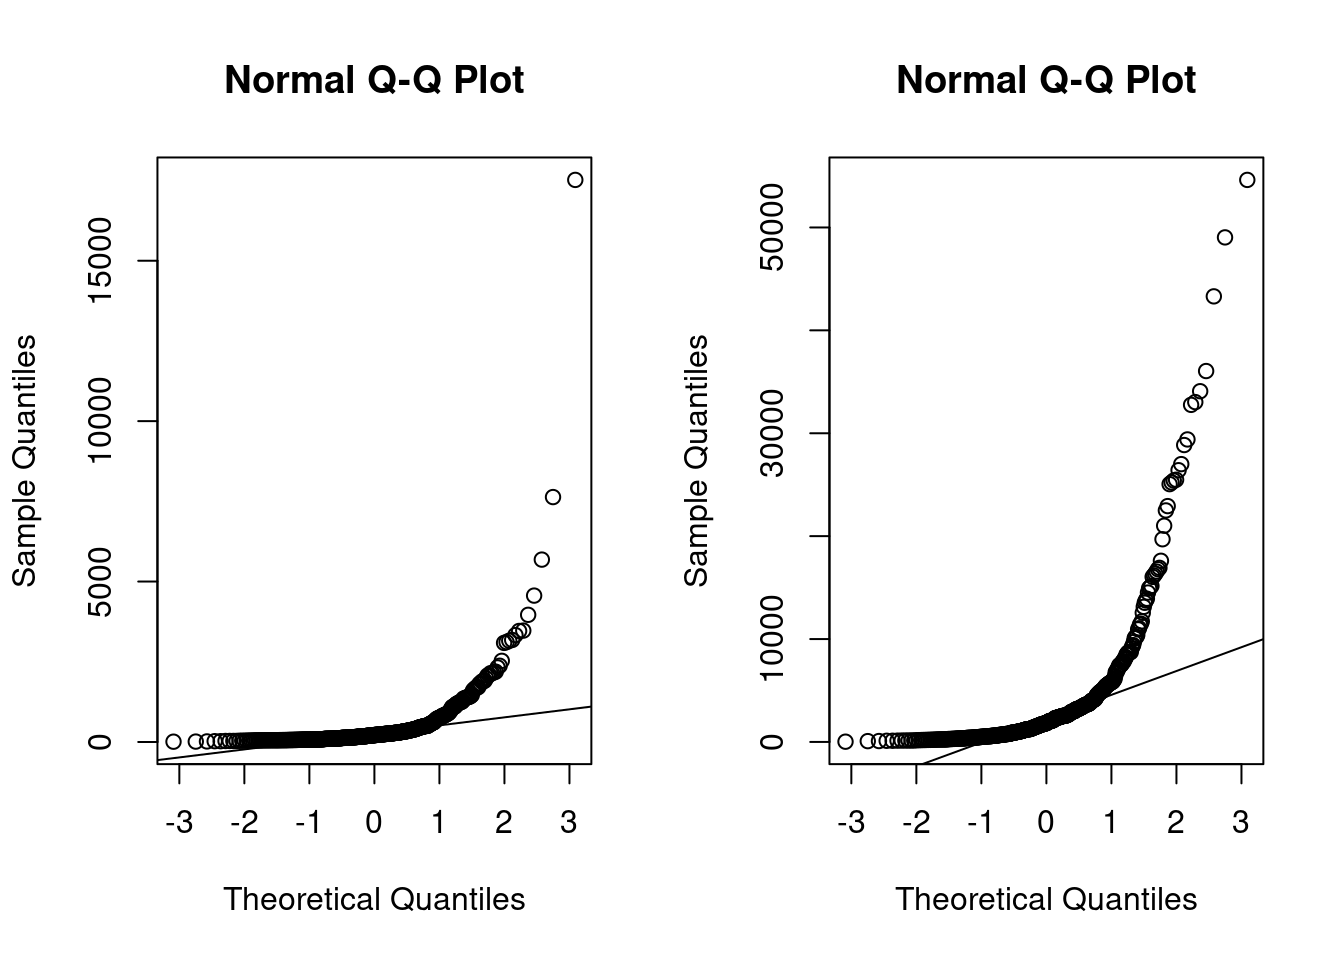
\includegraphics{DASE_files/figure-latex/unnamed-chunk-31-3.pdf}
* We observe the non-normality of the data. \\
\#\#\#\# Normality. Galton data \\
It is the data based on the famous 1885 Francis Galton's study about the relationship between the heights of adult children and the heights of their parents. \\
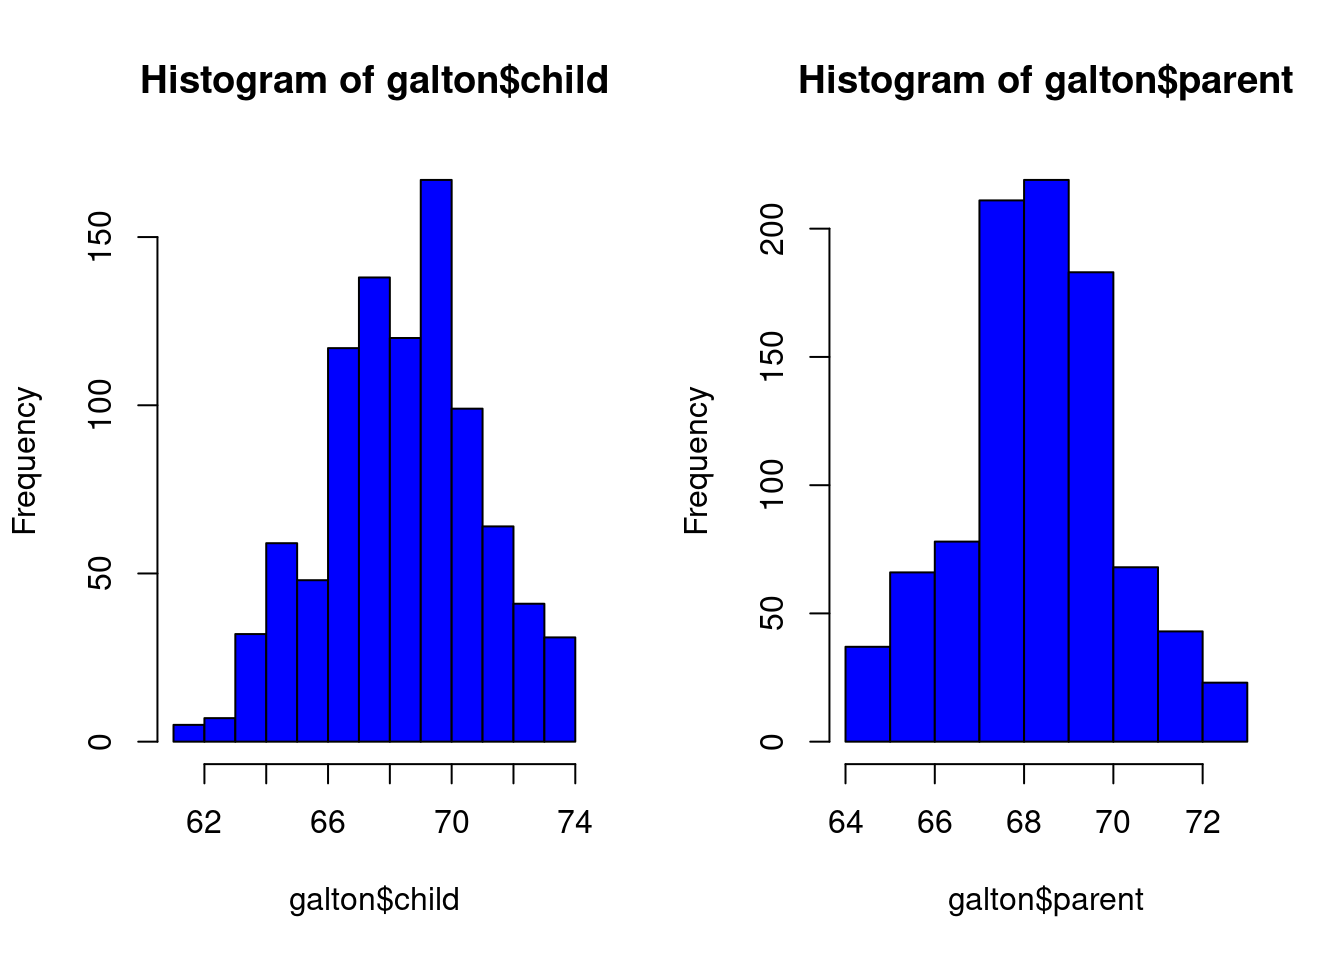
\includegraphics{DASE_files/figure-latex/galtonData-1.pdf} \\
\#\#\#\# Normalization \\
Take \(log\)s in both independent variables. For example, with the \emph{China} dataset. \\
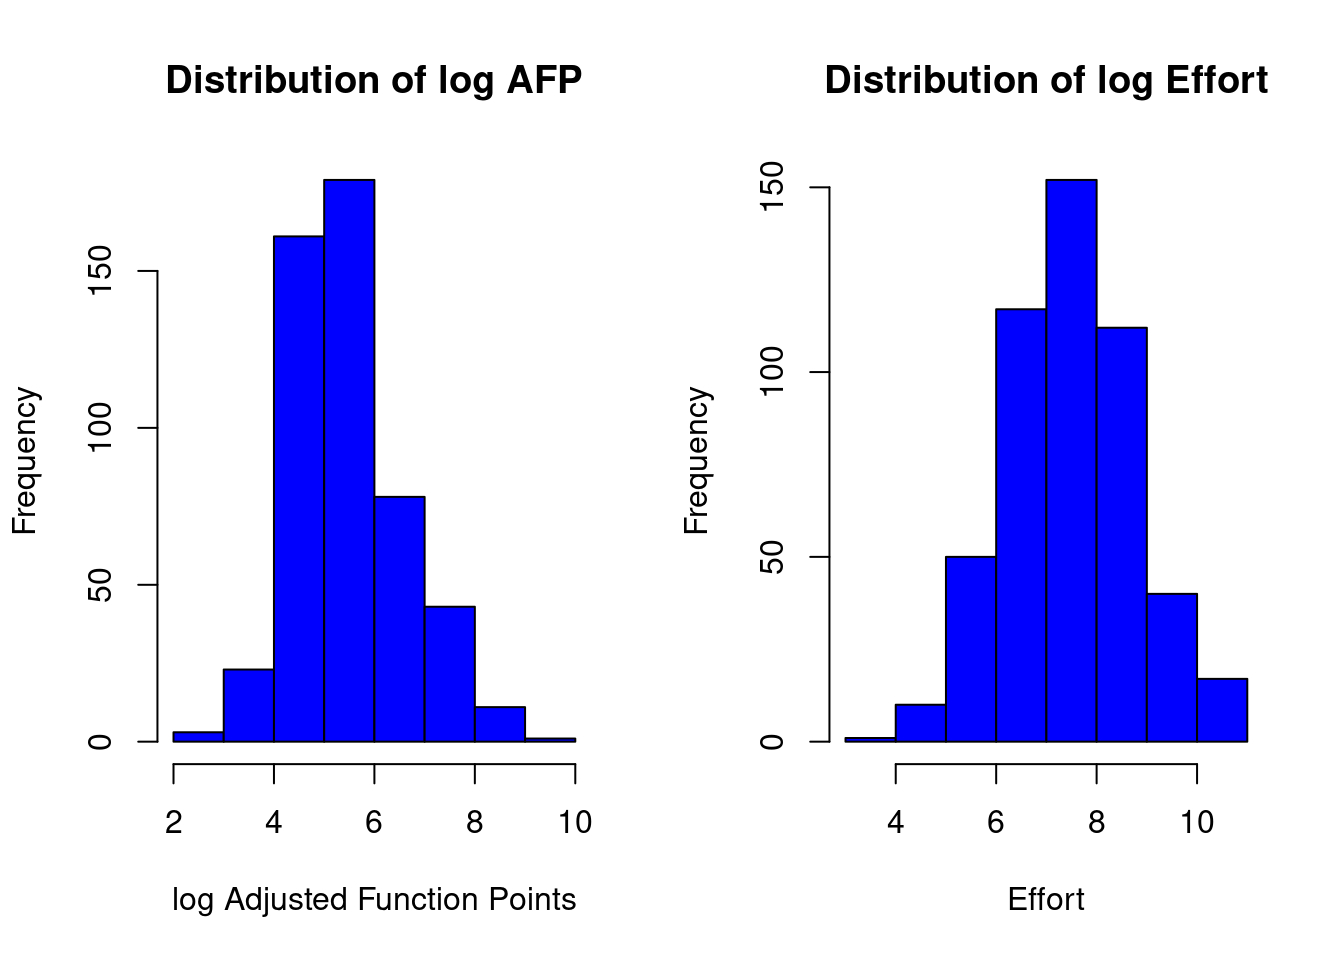
\includegraphics{DASE_files/figure-latex/logExample-1.pdf} 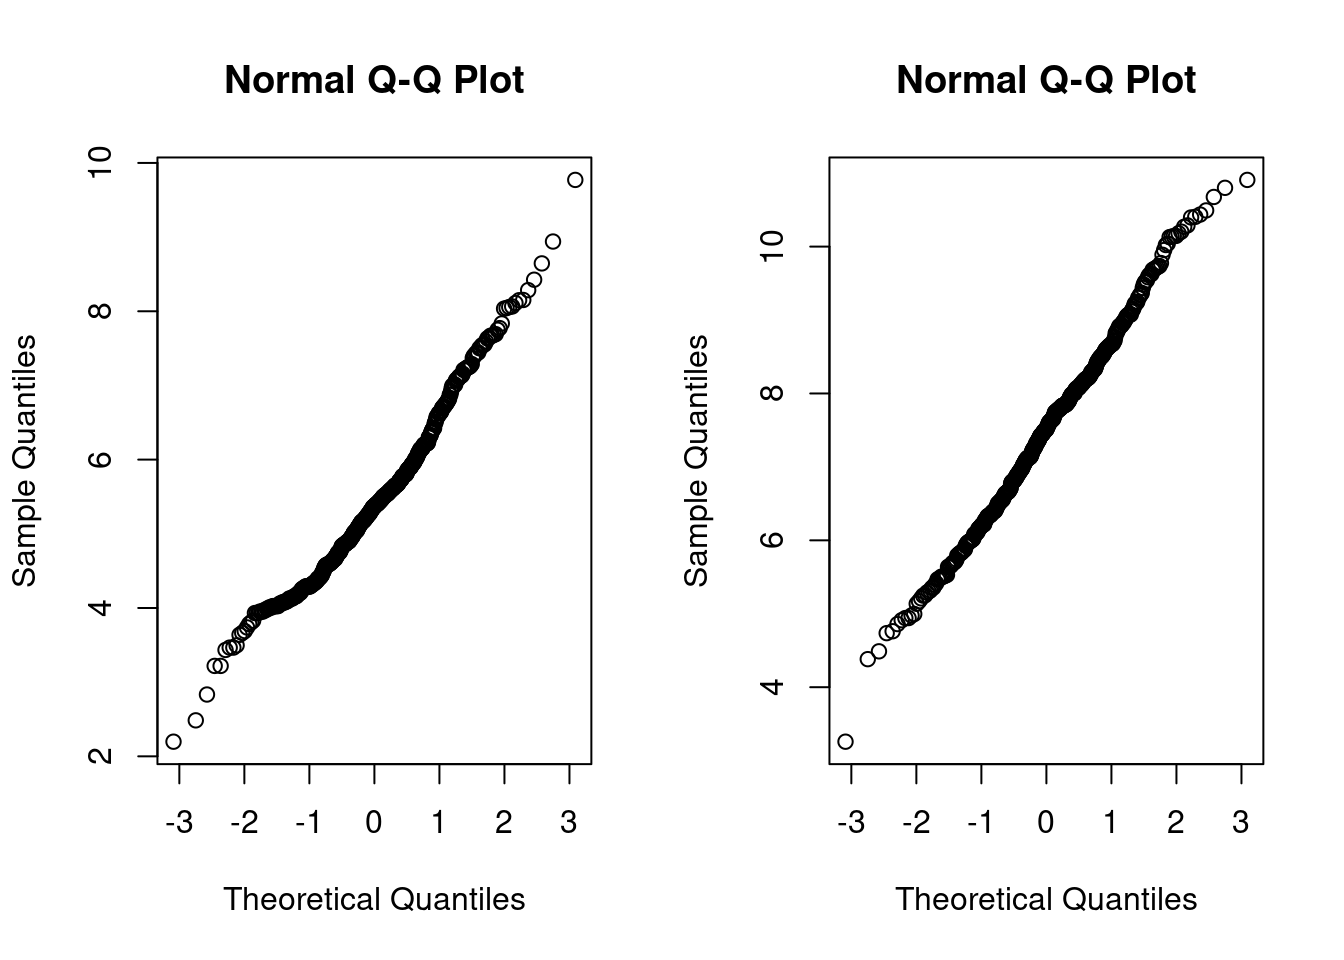
\includegraphics{DASE_files/figure-latex/logExample-2.pdf} \\
* If the \(log\) transformation is used, then the estimation equation is:
\(y= e^{b_0 + b_1 log(x)} \) \\
\#\# Correlation \\
\emph{Correlation} is a statistical relationship between two sets of data. With the whole dataset we may check for the linear Correlation of the variables we are interested in. \\
As an example with the China dataset \\
\texttt{r\ par(mfrow=c(1,1))\ plot(china\_size,china\_effort)} \\
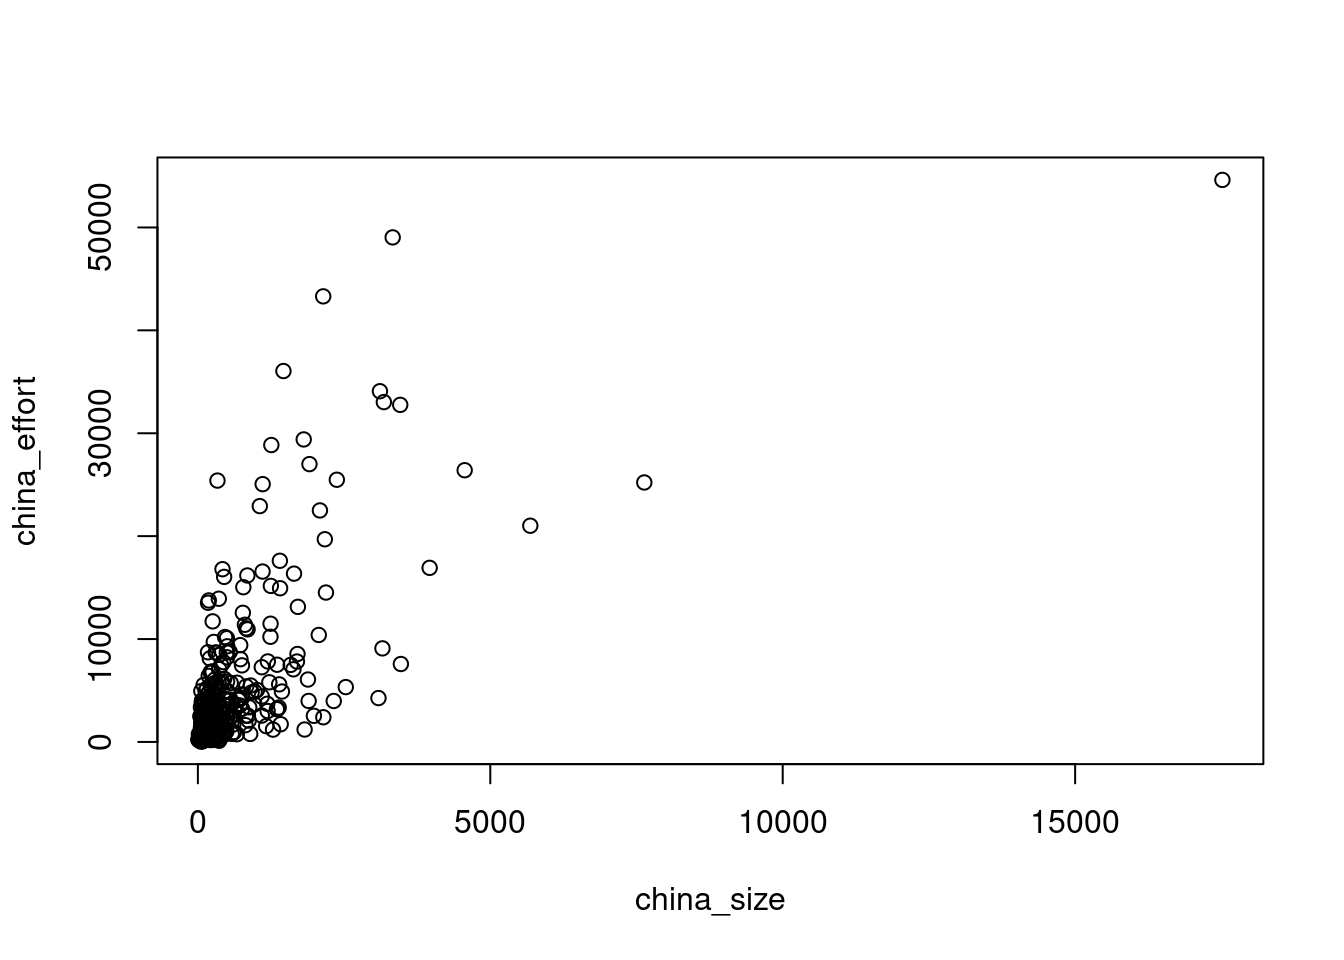
\includegraphics{DASE_files/figure-latex/correlationChinaDataset-1.pdf} \\
\texttt{r\ cor(china\_size,china\_effort)} \\
\texttt{\#\#\ {[}1{]}\ 0.685} \\
\texttt{r\ cor.test(china\_size,china\_effort)} \\
\texttt{\#\#\ \#\#\ \ Pearson\textquotesingle{}s\ product-moment\ correlation\ \#\#\ \#\#\ data:\ \ china\_size\ and\ china\_effort\ \#\#\ t\ =\ 21,\ df\ =\ 497,\ p-value\ \textless{}2e-16\ \#\#\ alternative\ hypothesis:\ true\ correlation\ is\ not\ equal\ to\ 0\ \#\#\ 95\ percent\ confidence\ interval:\ \#\#\ \ 0.635\ 0.729\ \#\#\ sample\ estimates:\ \#\#\ \ \ cor\ \#\#\ 0.685} \\
\texttt{r\ cor(china\_size,china\_effort,\ method="spearman")} \\
\texttt{\#\#\ {[}1{]}\ 0.649} \\
\texttt{r\ cor(china\_size,china\_effort,\ method="kendall")} \\
\texttt{\#\#\ {[}1{]}\ 0.468} \\
\#\# Confidence Intervals. Bootstrap
* Until now we have generated point estimates
* A \emph{confidence interval} (CI) is an interval estimate of a population parameter. The parameter can be the mean, the median or other. The frequentist CI is an observed interval that is different from sample to sample. It frequently includes the value of the unobservable parameter of interest if the experiment is repeated. The \emph{confidence level} is the value that measures the frequency that the constructed intervals contain the true value of the parameter.
* The construction of a confidence interval with an exact value of confidence level for a distribution requires some statistical properties. Usually, \emph{normality} is one of the properties required for computing confidence intervals.
+ Not all confidence intervals contain the true value of the parameter.
+ Simulation of confidence intervals \\
An example from Ugarte et al. \citep{ugarte2015probability} \\
\texttt{r\ set.seed(10)\ norsim(sims\ =\ 100,\ n\ =\ 36,\ mu\ =\ 100,\ sigma\ =\ 18,\ conf.level\ =\ 0.95)} \\
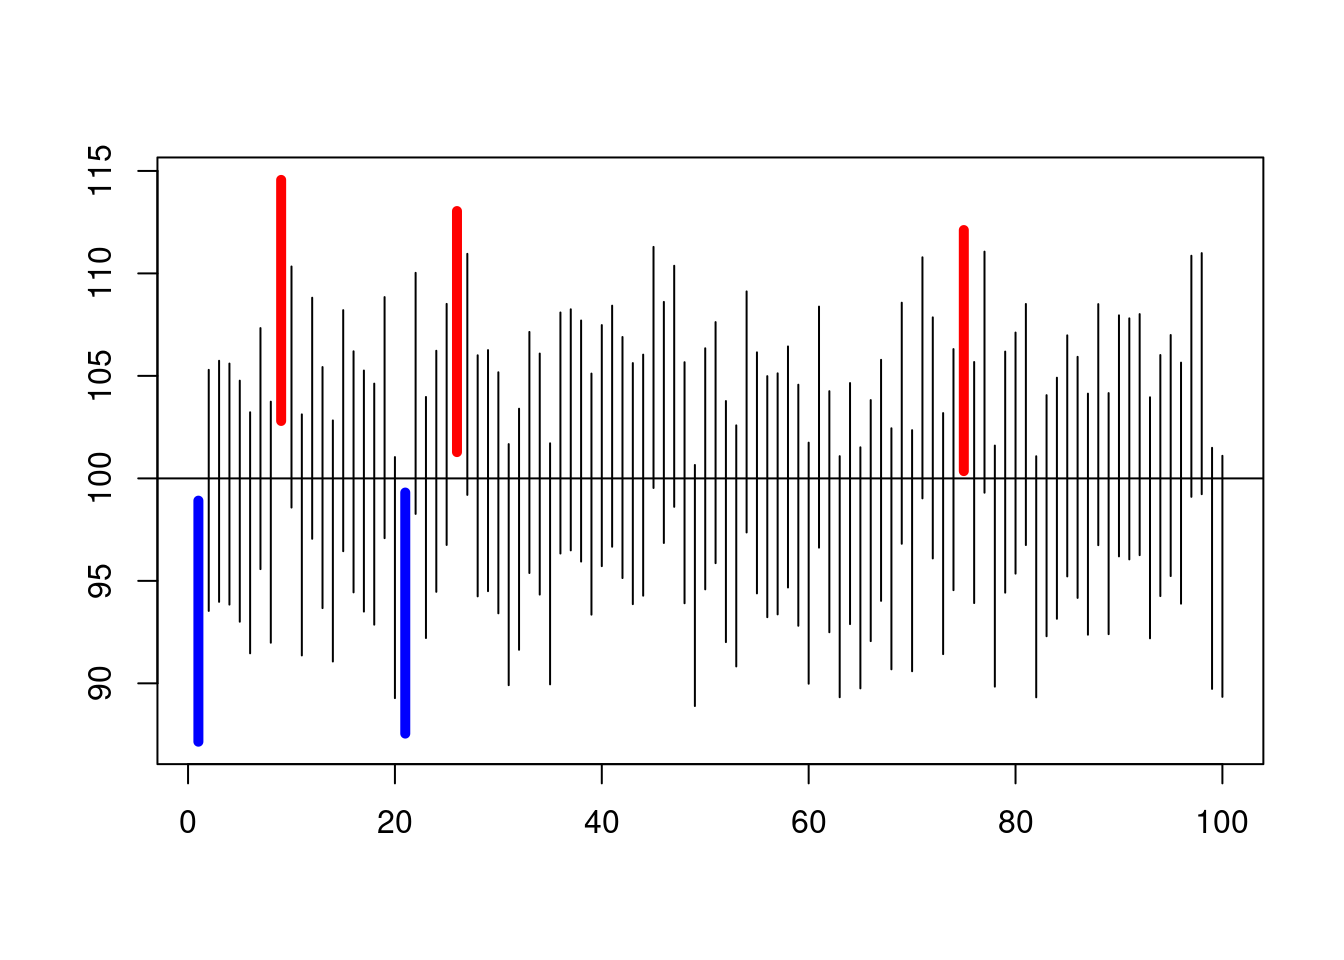
\includegraphics{DASE_files/figure-latex/unnamed-chunk-32-1.pdf} \\
* The range defined by the confidence interval will vary with each sample, because the sample size will vary each time and the standard deviation will vary too.
* 95\% confidence interval: it is the probability that the hypothetical confidence intervals (that would be computed from the hypothetical repeated samples) will contain the population mean.
* the particular interval that we compute on one sample does not mean that the population mean lies within that interval with a probability of 95\%.
* Recommended reading: \citep{Hoekstra2014} \emph{Robust misinterpretation of confidence intervals} \\
\#\# Nonparametric Bootstrap
* For computing CIs the important thing is to know the assumptions that are made to ``know'' the
distribution of the statistic.
* There is a way to compute confidence intervals without meeting the requirements of parametric methods.
* \textbf{Resampling} or \textbf{bootstraping} is a method to calculate estimates of a parameter taking samples from the original data and using those \emph{resamples} to calculate statistics. Using the resamples usually gives more accurate results than using the original single sample to calculate an estimate of a parameter. \\
\includegraphics{figures/bootstrap.png}
- An example of bootstrap CI can be found in Chapter \ref{evaluationSE}, ``Evaluation in Software Engineering'' \\
 \\
\# Classical Hypothesis Testing \\
- By ``classical'' we mean the standard ``frequentist'' approach to hypothesis testing. The ``frequentist'' approach to probability sees it as the frequency of events in the long run. We repeat experiments over and over and we count the times that our object of interest appears in the sequence. \\
- The classical approach is usually called \textbf{null hypothesis significance testing} (NHST) because the process starts by setting a null hypothesis \(H_0\) which is the opposite about what we think is true. \\
- The rationale of the process is that the statistical hypothesis should be \emph{falsifiable}, that is, we can find evidence that the hypothesis is not true. We try to find evidence against the null hypothesis in order to support our alternative hypothesis \(H_A\) \\
- Usually, the null hypothesis is described as the situation of ``no effect'' and the alternative hypothesis describes the effect that we are looking for. \\
- After collecting data, taking an actual sample, we measure the distance of our parameter of interest from the hypothesized population parameter, and use the facts of the sampling distribution to determine the probability of obtaining such a sample \emph{assuming the hypothesis is true}. This is amounts to a test of the hypothesis. \\
- If the probability of our sample, given the null hypothesis is high, this provides evidence that the null hypothesis is true. Conversely, if the probability of the sample is low (given the hypothesis), this is evidence against the null hypothesis. The hypothesis being tested in this way is named the \emph{null hypothesis}. \\
- The goal of the test is to determine if the null hypothesis can be rejected. A statistical test can either reject or fail to reject a null hypothesis, but never prove it true. \\
- We can make two types of errors: false positive (Type I) and false negative (Type II) \\
- Type I and Type II errors \\
\includegraphics{figures/typeIandIIwiki.png} \\
- Two-tailed NHST \\
\includegraphics{figures/stat_power_ggplot.png} \\
- One-tailed NHST \\
\includegraphics{figures/One-tailedNHST.png} \\
- elementary example \\
\texttt{r\ data\ =\ c(52.7,\ 53.9,\ 41.7,\ 71.5,\ 47.6,\ 55.1,\ 62.2,\ 56.5,\ 33.4,\ 61.8,\ 54.3,\ 50.0,\ 45.3,\ 63.4,\ 53.9,\ 65.5,\ 66.6,\ 70.0,\ 52.4,\ 38.6,\ 46.1,\ 44.4,\ 60.7,\ 56.4);\ t.test(data,\ mu=50,\ alternative\ =\ \textquotesingle{}greater\textquotesingle{})} \\
\texttt{\#\#\ \#\#\ \ One\ Sample\ t-test\ \#\#\ \#\#\ data:\ \ data\ \#\#\ t\ =\ 2,\ df\ =\ 23,\ p-value\ =\ 0.02\ \#\#\ alternative\ hypothesis:\ true\ mean\ is\ greater\ than\ 50\ \#\#\ 95\ percent\ confidence\ interval:\ \#\#\ \ 50.9\ \ Inf\ \#\#\ sample\ estimates:\ \#\#\ mean\ of\ x\ \#\#\ \ \ \ \ \ 54.3} \\
- Keeping this simple, we could start hypothesis testing about one sample median with the wilcoxon test for non-normal distributions. \\
- ``ae'' is the absolute error in the China Test data \\
\texttt{r\ median(ae)} \\
\texttt{\#\#\ {[}1{]}\ 867} \\
\texttt{r\ mean(ae)} \\
\texttt{\#\#\ {[}1{]}\ 1867} \\
\texttt{r\ wilcox.test(ae,\ mu=800,\ alternative\ =\ \textquotesingle{}greater\textquotesingle{})\ \#change\ the\ values\ of\ mu\ and\ see\ the\ results} \\
\texttt{\#\#\ \#\#\ \ Wilcoxon\ signed\ rank\ test\ with\ continuity\ correction\ \#\#\ \#\#\ data:\ \ ae\ \#\#\ V\ =\ 8990,\ p-value\ =\ 8e-04\ \#\#\ alternative\ hypothesis:\ true\ location\ is\ greater\ than\ 800} \\
- Quick introduction at \url{https://psychstatsworkshop.wordpress.com/2014/08/06/lesson-9-hypothesis-testing/} \\
\#\# p-values
- p-value: the p-value of a statistical test is the probability, computed assuming that \(H_0\) is true, that the test statistic would take a value as extreme or more extreme than that actually observed.
- \url{http://www.nature.com/news/psychology-journal-bans-p-values-1.17001}
- \url{https://www.sciencenews.org/blog/context/p-value-ban-small-step-journal-giant-leap-science} \\
\includegraphics{figures/pvalueBan.png} \\
 \\
\# (PART) Preprocessing \{-\} \\
\# Preprocessing \\
Following the data mining process, we describe what is meant by preprocessing, classical supervised models, unsupervised models and evaluation in the context of software engineering with examples \\
This task is probably the hardest and where most of effort is spend in the data mining process. It is quite typical to transform the data, for example, finding inconsistencies, normalising, imputing missing values, transforming input data, merging variables, etc. \\
Typically, pre-processing consist of the following tasks (subprocesses): \\
+ Data cleaning (consistency, noise detection, outliers)
+ Data integration
+ Data transformation (normalisation, discretisation) and derivation of new attributes from existing ones (e.g., population density from population and area)
+ Missing data imputation
+ Data reduction (feature selection and instace selection) \\
\#\# Data \\
\emph{Consistent} data are semantically correct based on real-world knowledge of the problem, i.e., no constrains are violated and data that can be used for inducing models and analysis. For example, the LoC or effort is constrained to non-negative values. We can also consider that to multiple attributes are consistent among them, and even datasets (e.g., same metrics but collected by different tools) \\
\#\# Missing values \\
\emph{Missing values} will have a negative effect when analysing the data or learning models. The results can be biased when compared with the models induced from the complete data, the results can be harder to analyse, it may be needed to discard records with missing values depending on the algorithm and this can be an important problems with small datasets such as the effort estimation ones. \\
Missing data is typically classified into:
* MCAR (Missing Completely at Random) or MAR (Missing At Random) where there is no reason for those missing values and we can assume that the distribution could follow the attribute's distribution.
* MNAR (Missing Not At Random) where there is a pattern for those missing values and it may may be advisable to check the data gathering process to try to understand why such information is missing. \\
\emph{Imputation} consists in replacing missing values for estimates of those missing values. Many algorithms do cannot handle missing values and therefore, imputation methods are needed. We can use simple approaches such as the replacing the missing values with the mean or mode of the attribute. More elaborated approaches include: \\
* EM (Expectation-Maximisation)
* Distance-based
+ \(k\)-NN (\(k\)-Nearest Neighbours)
+ Clustering \\
In R, a missing value is represented with \texttt{NA} and the analyst must decide what to do with missing data. The simplest approach is to leave out instances (ignore missing -IM-) with with missing data. This functionality is supported by many base functions through the \texttt{na.rm} option. \\
The \texttt{mice} R package. MICE (Multivariate Imputation via Chained Equations) assumes that data are missing at random. Other packages include \texttt{Amelia}, \texttt{missForest}, \texttt{Hmisc} and \texttt{mi}. \\
\#\# Noise \\
Imperfections of the real-world data that influences negatively in the induced machine learning models. Approaches to deal with noisy data include:
* Robust learners capable of handling noisy data (e.g., C4.5 through pruning strategies)
* Data polishing methods which aim to correct noisy instances prior training
* Noise filters which are used to identify and eliminate noisy instances from the training data. \\
Types of noise data:
* Class Noise (aka label noise).
+ There can be contradictory cases (all attributes have the same value except the class)
+ Misclassifications. The class attribute is not labeled with the true label (golden truth)
* Attribute Noise. Values of attributes that are noise, missing or unknown. \\
\#\# Outliers \\
There is a large amount of literature related to outlier detection, and furthermore several definitions of outlier exist. \\
```r
library(DMwR2)
library(foreign) \\
kc1 \textless- read.arff(``./datasets/defectPred/D1/KC1.arff'')
``` \\
The LOF algorithm (\texttt{lofactor}), given a data set it produces a vector of local outlier factors for each case. \\
\texttt{r\ kc1num\ \textless{}-\ kc1{[},1:21{]}\ outlier.scores\ \textless{}-\ lofactor(kc1num,\ k=5)\ plot(density(na.omit(outlier.scores)))} \\
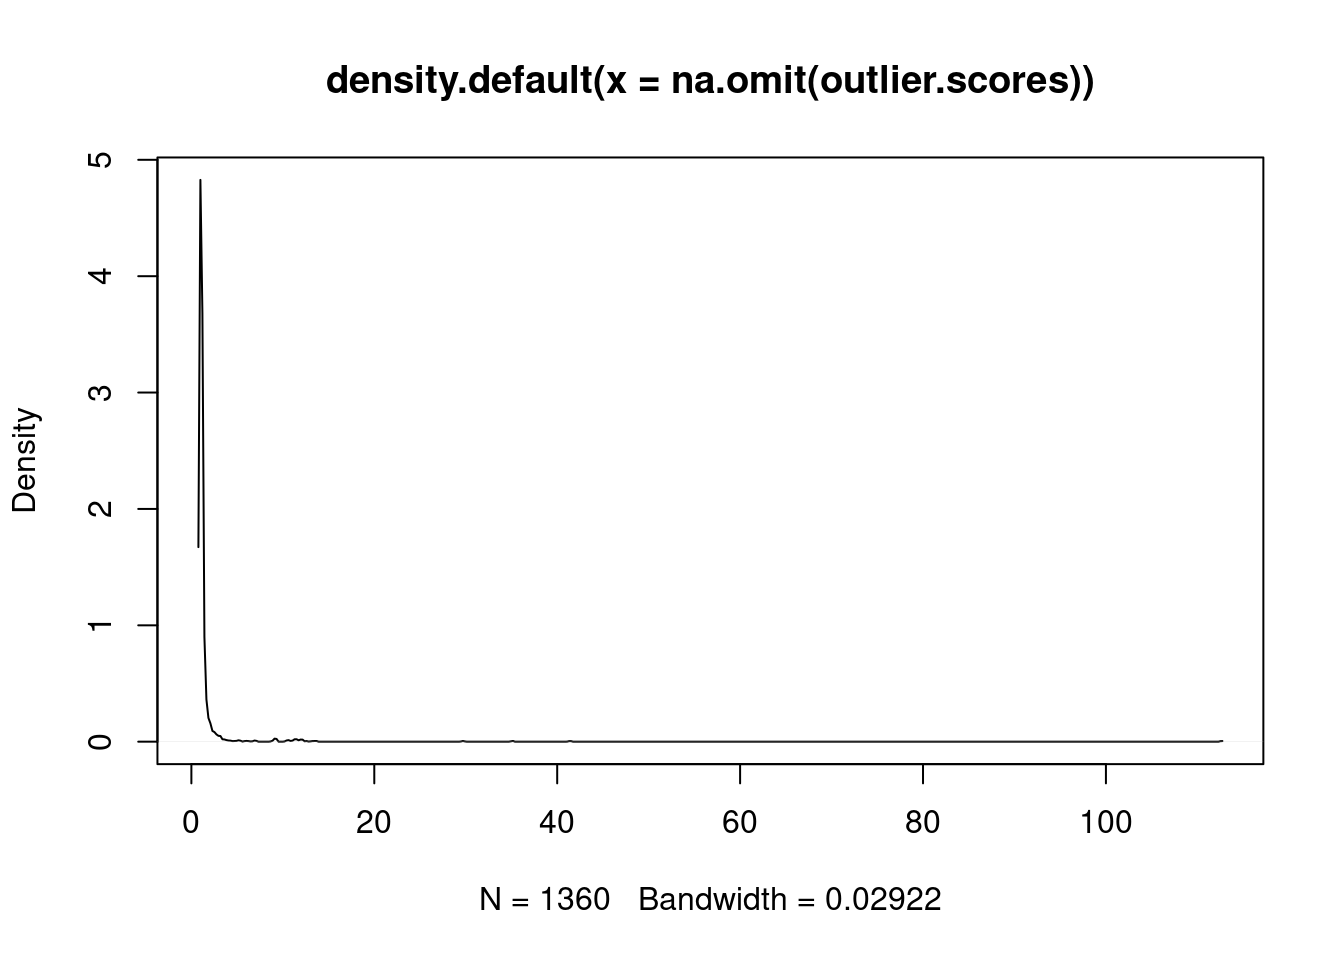
\includegraphics{DASE_files/figure-latex/unnamed-chunk-37-1.pdf} \\
\texttt{r\ outliers\ \textless{}-\ order(outlier.scores,\ decreasing=T){[}1:5{]}\ print(outliers)} \\
\texttt{\#\#\ {[}1{]}\ \ 1\ \ 6\ 14\ 31\ 33} \\
Another simple method of Hiridoglou and Berthelot for positive observations. \\
\#\# Feature selection \\
Feature Selection (FS) aims at identifying the most relevant attributes from a dataset. It is important in different ways: \\
* A reduced volume of data allows different data mining or searching techniques to be applied. \\
* Irrelevant and redundant attributes can generate less accurate and more complex models. Furthermore, data mining algorithms can be executed faster. \\
* It avoids the collection of data for those irrelevant and redundant attributes in the future. \\
The problem of FS received a thorough treatment in pattern recognition and machine learning. Most of the FS algorithms tackle the task as a \emph{search} problem, where each
state in the search specifies a distinct subset of the possible attributes \citep{BL97}. The search procedure is combined with a criterion to evaluate the merit of each candidate subset of attributes. There are a multiple possible combinations between each procedure search and each attribute measure \citep{LY05}. \\
There are two major approaches in FS from the method's output point of view: \\
* \emph{Feature subset selection} (FSS) \\
* \emph{Feature ranking} in which attributes are ranked as a list of features which are ordered according to evaluation measures (a subset of features is often selected from the top of the ranking list). \\
FFS algorithms designed with different evaluation criteria broadly fall into two categories: \\
* The \emph{filter} model relies on general characteristics of the data to evaluate and select feature subsets without involving any data mining algorithm. \\
* The \emph{wrapper} model requires one predetermined mining algorithm and uses its performance as the evaluation criterion. It searches for features better suited to the mining algorithm aiming to improve mining performance, but it also tends to be more computationally expensive than filter model \citep[\citet{Lan94}]{KJ97}. \\
Feature subset algorithms search through candidate feature subsets guide by a certain evaluation measure \citep{LM98} which captures the goodness of each subset. An optimal (or near optimal) subset is selected when the search stops. \\
Some existing evaluation measures that have been shown effective in removing both irrelevant and redundant features include the consistency measure \citep{DLM00}, the correlation measure \citep{Hal99} and the estimated accuracy of a learning algorithm \citep{KJ97}. \\
+ \emph{Consistency} measure attempts to find a minimum number of features that separate classes as consistently as the full set of features can. An inconsistency is defined as to instances having the same
feature values but different class labels. \\
+ \emph{Correlation} measure evaluates the goodness of feature subsets based on the hypothesis that good feature subsets contain features highly correlated to the class, yet uncorrelated to each other. \\
+ \emph{Wrapper-based} attribute selection uses the target learning algorithm to estimate the worth of attribute subsets. The feature subset selection algorithm conducts a search for a good subset using
the induction algorithm itself as part of the evaluation function. \\
Langley \citeyearpar{Lan94} notes that feature selection algorithms that search through the space of feature subsets must address four main issues: (i) the starting point of the search, (ii) the organization of the search, (iii) the evaluation of features subsets and (iv) the criterion used to terminate the search. Different algorithms address theses issues differently. \\
It is impractical to look at all possible feature subsets, even with a small number of attributes. Feature selection algorithms usually proceed greedily and are be classified into those that add features to an initially empty set (\emph{forward selection}) and those that remove features from an initially complete set (\emph{backwards elimination}). Hybrids both add and remove features as the algorithm progresses. Forward selection is much faster than backward elimination and therefore scales better to large data sets. A wide range of search strategies can be used: best-first, branch-and-bound, simulated annealing, genetic algorithms (see Kohavi and John \citeyearpar{KJ97} for a review). \\
\#\#\# FSelector package in R \\
The FSelector package in R implements many algorithms available in Weka \\
```r
library(FSelector)
library(foreign) \\
cm1 \textless- read.arff(``./datasets/defectPred/D1/CM1.arff'') \\
cm1RFWeigths \textless- random.forest.importance(Defective \textasciitilde{} ., cm1)
cutoff.biggest.diff(cm1RFWeigths)
``` \\
\texttt{\#\#\ {[}1{]}\ "LOC\_COMMENTS"\ \ \ \ \ \ \ \ \ "NUM\_UNIQUE\_OPERATORS"} \\
Using the Information Gain measure as ranking: \\
\texttt{r\ cm1GRWeights\ \textless{}-\ gain.ratio(Defective\ \textasciitilde{}\ .,\ cm1)\ cm1GRWeights} \\
\texttt{\#\#\ \ \ \ \ \ \ \ \ \ \ \ \ \ \ \ \ \ \ \ \ \ \ \ \ \ \ \ \ \ \ \ \ attr\_importance\ \#\#\ LOC\_BLANK\ \ \ \ \ \ \ \ \ \ \ \ \ \ \ \ \ \ \ \ \ \ \ \ \ \ \ \ \ \ \ \ 0.0000\ \#\#\ BRANCH\_COUNT\ \ \ \ \ \ \ \ \ \ \ \ \ \ \ \ \ \ \ \ \ \ \ \ \ \ \ \ \ 0.0000\ \#\#\ CALL\_PAIRS\ \ \ \ \ \ \ \ \ \ \ \ \ \ \ \ \ \ \ \ \ \ \ \ \ \ \ \ \ \ \ 0.0000\ \#\#\ LOC\_CODE\_AND\_COMMENT\ \ \ \ \ \ \ \ \ \ \ \ \ \ \ \ \ \ \ \ \ 0.0000\ \#\#\ LOC\_COMMENTS\ \ \ \ \ \ \ \ \ \ \ \ \ \ \ \ \ \ \ \ \ \ \ \ \ \ \ \ \ 0.0754\ \#\#\ CONDITION\_COUNT\ \ \ \ \ \ \ \ \ \ \ \ \ \ \ \ \ \ \ \ \ \ \ \ \ \ 0.0000\ \#\#\ CYCLOMATIC\_COMPLEXITY\ \ \ \ \ \ \ \ \ \ \ \ \ \ \ \ \ \ \ \ 0.0000\ \#\#\ CYCLOMATIC\_DENSITY\ \ \ \ \ \ \ \ \ \ \ \ \ \ \ \ \ \ \ \ \ \ \ 0.0000\ \#\#\ DECISION\_COUNT\ \ \ \ \ \ \ \ \ \ \ \ \ \ \ \ \ \ \ \ \ \ \ \ \ \ \ 0.0000\ \#\#\ DECISION\_DENSITY\ \ \ \ \ \ \ \ \ \ \ \ \ \ \ \ \ \ \ \ \ \ \ \ \ 0.0000\ \#\#\ DESIGN\_COMPLEXITY\ \ \ \ \ \ \ \ \ \ \ \ \ \ \ \ \ \ \ \ \ \ \ \ 0.0000\ \#\#\ DESIGN\_DENSITY\ \ \ \ \ \ \ \ \ \ \ \ \ \ \ \ \ \ \ \ \ \ \ \ \ \ \ 0.0000\ \#\#\ EDGE\_COUNT\ \ \ \ \ \ \ \ \ \ \ \ \ \ \ \ \ \ \ \ \ \ \ \ \ \ \ \ \ \ \ 0.0000\ \#\#\ ESSENTIAL\_COMPLEXITY\ \ \ \ \ \ \ \ \ \ \ \ \ \ \ \ \ \ \ \ \ 0.0000\ \#\#\ ESSENTIAL\_DENSITY\ \ \ \ \ \ \ \ \ \ \ \ \ \ \ \ \ \ \ \ \ \ \ \ 0.0000\ \#\#\ LOC\_EXECUTABLE\ \ \ \ \ \ \ \ \ \ \ \ \ \ \ \ \ \ \ \ \ \ \ \ \ \ \ 0.0888\ \#\#\ PARAMETER\_COUNT\ \ \ \ \ \ \ \ \ \ \ \ \ \ \ \ \ \ \ \ \ \ \ \ \ \ 0.0000\ \#\#\ HALSTEAD\_CONTENT\ \ \ \ \ \ \ \ \ \ \ \ \ \ \ \ \ \ \ \ \ \ \ \ \ 0.0701\ \#\#\ HALSTEAD\_DIFFICULTY\ \ \ \ \ \ \ \ \ \ \ \ \ \ \ \ \ \ \ \ \ \ 0.0000\ \#\#\ HALSTEAD\_EFFORT\ \ \ \ \ \ \ \ \ \ \ \ \ \ \ \ \ \ \ \ \ \ \ \ \ \ 0.0375\ \#\#\ HALSTEAD\_ERROR\_EST\ \ \ \ \ \ \ \ \ \ \ \ \ \ \ \ \ \ \ \ \ \ \ 0.0448\ \#\#\ HALSTEAD\_LENGTH\ \ \ \ \ \ \ \ \ \ \ \ \ \ \ \ \ \ \ \ \ \ \ \ \ \ 0.0425\ \#\#\ HALSTEAD\_LEVEL\ \ \ \ \ \ \ \ \ \ \ \ \ \ \ \ \ \ \ \ \ \ \ \ \ \ \ 0.0000\ \#\#\ HALSTEAD\_PROG\_TIME\ \ \ \ \ \ \ \ \ \ \ \ \ \ \ \ \ \ \ \ \ \ \ 0.0375\ \#\#\ HALSTEAD\_VOLUME\ \ \ \ \ \ \ \ \ \ \ \ \ \ \ \ \ \ \ \ \ \ \ \ \ \ 0.0471\ \#\#\ MAINTENANCE\_SEVERITY\ \ \ \ \ \ \ \ \ \ \ \ \ \ \ \ \ \ \ \ \ 0.0000\ \#\#\ MODIFIED\_CONDITION\_COUNT\ \ \ \ \ \ \ \ \ \ \ \ \ \ \ \ \ 0.0000\ \#\#\ MULTIPLE\_CONDITION\_COUNT\ \ \ \ \ \ \ \ \ \ \ \ \ \ \ \ \ 0.0000\ \#\#\ NODE\_COUNT\ \ \ \ \ \ \ \ \ \ \ \ \ \ \ \ \ \ \ \ \ \ \ \ \ \ \ \ \ \ \ 0.0000\ \#\#\ NORMALIZED\_CYLOMATIC\_COMPLEXITY\ \ \ \ \ \ \ \ \ \ 0.0000\ \#\#\ NUM\_OPERANDS\ \ \ \ \ \ \ \ \ \ \ \ \ \ \ \ \ \ \ \ \ \ \ \ \ \ \ \ \ 0.0000\ \#\#\ NUM\_OPERATORS\ \ \ \ \ \ \ \ \ \ \ \ \ \ \ \ \ \ \ \ \ \ \ \ \ \ \ \ 0.0471\ \#\#\ NUM\_UNIQUE\_OPERANDS\ \ \ \ \ \ \ \ \ \ \ \ \ \ \ \ \ \ \ \ \ \ 0.0589\ \#\#\ NUM\_UNIQUE\_OPERATORS\ \ \ \ \ \ \ \ \ \ \ \ \ \ \ \ \ \ \ \ \ 0.0616\ \#\#\ NUMBER\_OF\_LINES\ \ \ \ \ \ \ \ \ \ \ \ \ \ \ \ \ \ \ \ \ \ \ \ \ \ 0.0573\ \#\#\ PERCENT\_COMMENTS\ \ \ \ \ \ \ \ \ \ \ \ \ \ \ \ \ \ \ \ \ \ \ \ \ 0.0663\ \#\#\ LOC\_TOTAL\ \ \ \ \ \ \ \ \ \ \ \ \ \ \ \ \ \ \ \ \ \ \ \ \ \ \ \ \ \ \ \ 0.0763} \\
\texttt{r\ cutoff.biggest.diff(cm1GRWeights)} \\
\texttt{\#\#\ \ {[}1{]}\ "LOC\_EXECUTABLE"\ \ \ \ \ \ \ "LOC\_TOTAL"\ \ \ \ \ \ \ \ \ \ \ \ "LOC\_COMMENTS"\ \#\#\ \ {[}4{]}\ "HALSTEAD\_CONTENT"\ \ \ \ \ "PERCENT\_COMMENTS"\ \ \ \ \ "NUM\_UNIQUE\_OPERATORS"\ \#\#\ \ {[}7{]}\ "NUM\_UNIQUE\_OPERANDS"\ \ "NUMBER\_OF\_LINES"\ \ \ \ \ \ "HALSTEAD\_VOLUME"\ \#\#\ {[}10{]}\ "NUM\_OPERATORS"\ \ \ \ \ \ \ \ "HALSTEAD\_ERROR\_EST"\ \ \ "HALSTEAD\_LENGTH"\ \#\#\ {[}13{]}\ "HALSTEAD\_EFFORT"\ \ \ \ \ \ "HALSTEAD\_PROG\_TIME"} \\
\texttt{r\ \#\ After\ assigning\ weights,\ we\ can\ select\ the\ statistaclly\ significant\ ones\ cm1X2Weights\ \textless{}-\ chi.squared(Defective\ \textasciitilde{}\ .,\ cm1)\ cutoff.biggest.diff(cm1X2Weights)} \\
\texttt{\#\#\ \ {[}1{]}\ "LOC\_EXECUTABLE"\ \ \ \ \ \ \ "LOC\_COMMENTS"\ \ \ \ \ \ \ \ \ "LOC\_TOTAL"\ \#\#\ \ {[}4{]}\ "NUM\_UNIQUE\_OPERATORS"\ "NUM\_UNIQUE\_OPERANDS"\ \ "NUMBER\_OF\_LINES"\ \#\#\ \ {[}7{]}\ "HALSTEAD\_VOLUME"\ \ \ \ \ \ "NUM\_OPERATORS"\ \ \ \ \ \ \ \ "HALSTEAD\_ERROR\_EST"\ \#\#\ {[}10{]}\ "HALSTEAD\_CONTENT"\ \ \ \ \ "HALSTEAD\_EFFORT"\ \ \ \ \ \ "HALSTEAD\_PROG\_TIME"\ \#\#\ {[}13{]}\ "HALSTEAD\_LENGTH"\ \ \ \ \ \ "PERCENT\_COMMENTS"} \\
Using CFS attribute selection \\
```r
library(FSelector)
library(foreign) \\
cm1 \textless- read.arff(``./datasets/defectPred/D1/CM1.arff'') \\
result \textless- cfs(Defective \textasciitilde{} ., cm1)
f \textless- as.simple.formula(result, ``Defective'')
f
``` \\
\texttt{\#\#\ Defective\ \textasciitilde{}\ LOC\_COMMENTS\ +\ LOC\_EXECUTABLE\ +\ HALSTEAD\_CONTENT\ +\ \#\#\ \ \ \ \ NUM\_UNIQUE\_OPERATORS\ +\ PERCENT\_COMMENTS\ \#\#\ \textless{}environment:\ 0x55d7e72edbe0\textgreater{}} \\
Other packages for Feature selection in R include \texttt{FSelectorRccp} which re-implments the FSlector without WEKA dependencies. \\
Another popular package is \texttt{Boruta}, which is based on selection based on Random Forest. \\
\#\# Instance selection \\
Removal of samples (complementary to the removal of attributes) in order to scale down the dataset prior to learning a model so that there is (almost) no performance loss. \\
There are two types of processes: \\
* \emph{Prototype Selection} (PS) \citep{GDCH12} when the subset is used with a distance based method (kNN) \\
* \emph{Training Set Selection} (TSS) \citep{CanoHL07} in which an actual model is learned. \\
It is also a search problem as with \emph{feature selection}. Garcia et al. \citeyearpar{GDCH12} provide a comprehensive overview of the topic. \\
\#\# Discretization \\
This process transforms continuous attributes into discrete ones, by associating categorical values to intervals and thus transforming quantitative data into qualitative data. \\
\#\# Correlation Coefficient and Covariance for Numeric Data \\
Two random variables \(x\) and \(y\) are called independent if the probability distribution of one variable is not affected by the presence of another. \\
\(\tilde{\chi}^2=\frac{1}{d}\sum_{k=1}^{n} \frac{(O_k - E_k)^2}{E_k}\) \\
\texttt{r\ chisq.test(kc1\$LOC\_BLANK,kc1\$BRANCH\_TOTAL)} \\
\texttt{\#\#\ \#\#\ \ Chi-squared\ test\ for\ given\ probabilities\ \#\#\ \#\#\ data:\ \ kc1\$LOC\_BLANK\ \#\#\ X-squared\ =\ 17705,\ df\ =\ 2095,\ p-value\ \textless{}2e-16} \\
\texttt{r\ chisq.test(kc1\$DESIGN\_COMPLEXITY,kc1\$CYCLOMATIC\_COMPLEXITY)} \\
\texttt{\#\#\ \#\#\ \ Pearson\textquotesingle{}s\ Chi-squared\ test\ \#\#\ \#\#\ data:\ \ kc1\$DESIGN\_COMPLEXITY\ and\ kc1\$CYCLOMATIC\_COMPLEXITY\ \#\#\ X-squared\ =\ 25101,\ df\ =\ 696,\ p-value\ \textless{}2e-16} \\
\#\# Normalization \\
\#\#\# Min-Max Normalization \\
\(z_i=\frac{x_i-\min(x)}{\max(x)-\min(x)}\) \\
\texttt{r\ library(caret)\ preObj\ \textless{}-\ preProcess(kc1{[},\ -22{]},\ method=c("center",\ "scale"))} \\
\#\#\# Z-score normalization
TBD \\
\#\# Transformations \\
\#\#\# Linear Transformations and Quadratic Trans formations
TBD \\
\#\#\# Box-cox transformation
TBD \\
\#\#\# Nominal to Binary tranformations
TBD \\
\#\# Preprocessing in R \\
\#\#\# The \texttt{dplyr} package \\
The \emph{\href{https://cran.r-project.org/web/packages/dplyr/index.html}{dplyr}} package created by Hadley Wickham. Some functions are similar to SQL syntax. key functions in dplyr include: \\
+ select: select columns from a dataframe
+ filter: select rows from a dataframe
+ summarize: allows us to do summary stats based upon the grouped variable
+ group\_by: group by a factor variable
+ arrange: order the dataset
+ joins: as in sql left join \\
Tutorial:
\url{https://github.com/justmarkham/dplyr-tutorial} \\
Examples \\
\texttt{r\ library(dplyr)} \\
Describe the dataframe: \\
\texttt{r\ str(kc1)} \\
\texttt{\#\#\ \textquotesingle{}data.frame\textquotesingle{}:\ \ \ \ 2096\ obs.\ of\ \ 22\ variables:\ \#\#\ \ \$\ LOC\_BLANK\ \ \ \ \ \ \ \ \ \ \ \ :\ num\ \ 0\ 0\ 0\ 0\ 2\ 0\ 0\ 0\ 0\ 2\ ...\ \#\#\ \ \$\ BRANCH\_COUNT\ \ \ \ \ \ \ \ \ :\ num\ \ 1\ 1\ 1\ 1\ 1\ 1\ 1\ 1\ 1\ 1\ ...\ \#\#\ \ \$\ LOC\_CODE\_AND\_COMMENT\ :\ num\ \ 0\ 0\ 0\ 0\ 0\ 0\ 0\ 0\ 0\ 0\ ...\ \#\#\ \ \$\ LOC\_COMMENTS\ \ \ \ \ \ \ \ \ :\ num\ \ 0\ 0\ 0\ 0\ 0\ 0\ 0\ 0\ 0\ 0\ ...\ \#\#\ \ \$\ CYCLOMATIC\_COMPLEXITY:\ num\ \ 1\ 1\ 1\ 1\ 1\ 1\ 1\ 1\ 1\ 1\ ...\ \#\#\ \ \$\ DESIGN\_COMPLEXITY\ \ \ \ :\ num\ \ 1\ 1\ 1\ 1\ 1\ 1\ 1\ 1\ 1\ 1\ ...\ \#\#\ \ \$\ ESSENTIAL\_COMPLEXITY\ :\ num\ \ 1\ 1\ 1\ 1\ 1\ 1\ 1\ 1\ 1\ 1\ ...\ \#\#\ \ \$\ LOC\_EXECUTABLE\ \ \ \ \ \ \ :\ num\ \ 3\ 1\ 1\ 1\ 8\ 3\ 1\ 1\ 1\ 9\ ...\ \#\#\ \ \$\ HALSTEAD\_CONTENT\ \ \ \ \ :\ num\ \ 11.6\ 0\ 0\ 0\ 18\ ...\ \#\#\ \ \$\ HALSTEAD\_DIFFICULTY\ \ :\ num\ \ 2.67\ 0\ 0\ 0\ 3.5\ 2.67\ 0\ 0\ 0\ 3.75\ ...\ \#\#\ \ \$\ HALSTEAD\_EFFORT\ \ \ \ \ \ :\ num\ \ 82.3\ 0\ 0\ 0\ 220.9\ ...\ \#\#\ \ \$\ HALSTEAD\_ERROR\_EST\ \ \ :\ num\ \ 0.01\ 0\ 0\ 0\ 0.02\ 0.01\ 0\ 0\ 0\ 0.04\ ...\ \#\#\ \ \$\ HALSTEAD\_LENGTH\ \ \ \ \ \ :\ num\ \ 11\ 1\ 1\ 1\ 19\ 11\ 1\ 1\ 1\ 29\ ...\ \#\#\ \ \$\ HALSTEAD\_LEVEL\ \ \ \ \ \ \ :\ num\ \ 0.38\ 0\ 0\ 0\ 0.29\ 0.38\ 0\ 0\ 0\ 0.27\ ...\ \#\#\ \ \$\ HALSTEAD\_PROG\_TIME\ \ \ :\ num\ \ 4.57\ 0\ 0\ 0\ 12.27\ ...\ \#\#\ \ \$\ HALSTEAD\_VOLUME\ \ \ \ \ \ :\ num\ \ 30.9\ 0\ 0\ 0\ 63.1\ ...\ \#\#\ \ \$\ NUM\_OPERANDS\ \ \ \ \ \ \ \ \ :\ num\ \ 4\ 0\ 0\ 0\ 7\ 4\ 0\ 0\ 0\ 10\ ...\ \#\#\ \ \$\ NUM\_OPERATORS\ \ \ \ \ \ \ \ :\ num\ \ 7\ 1\ 1\ 1\ 12\ 7\ 1\ 1\ 1\ 19\ ...\ \#\#\ \ \$\ NUM\_UNIQUE\_OPERANDS\ \ :\ num\ \ 3\ 0\ 0\ 0\ 5\ 3\ 0\ 0\ 0\ 8\ ...\ \#\#\ \ \$\ NUM\_UNIQUE\_OPERATORS\ :\ num\ \ 4\ 1\ 1\ 1\ 5\ 4\ 1\ 1\ 1\ 6\ ...\ \#\#\ \ \$\ LOC\_TOTAL\ \ \ \ \ \ \ \ \ \ \ \ :\ num\ \ 5\ 3\ 3\ 3\ 12\ 5\ 3\ 3\ 3\ 13\ ...\ \#\#\ \ \$\ Defective\ \ \ \ \ \ \ \ \ \ \ \ :\ Factor\ w/\ 2\ levels\ "N","Y":\ 1\ 1\ 1\ 1\ 1\ 1\ 1\ 1\ 1\ 1\ ...} \\
\texttt{tbl\_df} creates a ``local data frame'' as a wrapper for better printing \\
\texttt{r\ kc1\_tbl\ \textless{}-\ tbl\_df(kc1)\ \#deprecated} \\
\texttt{\#\#\ Warning:\ \textasciigrave{}tbl\_df()\textasciigrave{}\ was\ deprecated\ in\ dplyr\ 1.0.0.\ \#\#\ Please\ use\ \textasciigrave{}tibble::as\_tibble()\textasciigrave{}\ instead.\ \#\#\ This\ warning\ is\ displayed\ once\ every\ 8\ hours.\ \#\#\ Call\ \textasciigrave{}lifecycle::last\_lifecycle\_warnings()\textasciigrave{}\ to\ see\ where\ this\ warning\ was\ generated.} \\
\texttt{r\ kc1\_tbl\ \textless{}-\ tibble(kc1)} \\
Filter: \\
\texttt{r\ \#\ Filter\ rows:\ use\ comma\ or\ \&\ to\ represent\ AND\ condition\ filter(kc1\_tbl,\ Defective\ ==\ "Y"\ \&\ LOC\_BLANK\ !=\ 0)} \\
\texttt{\#\#\ \#\ A\ tibble:\ 251\ x\ 22\ \#\#\ \ \ \ LOC\_BLANK\ BRANCH\_COUNT\ LOC\_CODE\_AND\_COMMENT\ LOC\_COMMENTS\ CYCLOMATIC\_COMPLEXI\textasciitilde{}\ \#\#\ \ \ \ \ \ \ \ \textless{}dbl\textgreater{}\ \ \ \ \ \ \ \ \textless{}dbl\textgreater{}\ \ \ \ \ \ \ \ \ \ \ \ \ \ \ \ \textless{}dbl\textgreater{}\ \ \ \ \ \ \ \ \textless{}dbl\textgreater{}\ \ \ \ \ \ \ \ \ \ \ \ \ \ \ \ \textless{}dbl\textgreater{}\ \#\#\ \ 1\ \ \ \ \ \ \ \ \ 6\ \ \ \ \ \ \ \ \ \ \ 21\ \ \ \ \ \ \ \ \ \ \ \ \ \ \ \ \ \ \ \ 0\ \ \ \ \ \ \ \ \ \ \ 10\ \ \ \ \ \ \ \ \ \ \ \ \ \ \ \ \ \ \ 11\ \#\#\ \ 2\ \ \ \ \ \ \ \ \ 5\ \ \ \ \ \ \ \ \ \ \ 15\ \ \ \ \ \ \ \ \ \ \ \ \ \ \ \ \ \ \ \ 0\ \ \ \ \ \ \ \ \ \ \ \ 2\ \ \ \ \ \ \ \ \ \ \ \ \ \ \ \ \ \ \ \ 8\ \#\#\ \ 3\ \ \ \ \ \ \ \ \ 2\ \ \ \ \ \ \ \ \ \ \ \ 5\ \ \ \ \ \ \ \ \ \ \ \ \ \ \ \ \ \ \ \ 0\ \ \ \ \ \ \ \ \ \ \ \ 0\ \ \ \ \ \ \ \ \ \ \ \ \ \ \ \ \ \ \ \ 3\ \#\#\ \ 4\ \ \ \ \ \ \ \ \ 4\ \ \ \ \ \ \ \ \ \ \ \ 5\ \ \ \ \ \ \ \ \ \ \ \ \ \ \ \ \ \ \ \ 0\ \ \ \ \ \ \ \ \ \ \ \ 2\ \ \ \ \ \ \ \ \ \ \ \ \ \ \ \ \ \ \ \ 3\ \#\#\ \ 5\ \ \ \ \ \ \ \ \ 2\ \ \ \ \ \ \ \ \ \ \ 11\ \ \ \ \ \ \ \ \ \ \ \ \ \ \ \ \ \ \ \ 0\ \ \ \ \ \ \ \ \ \ \ \ 2\ \ \ \ \ \ \ \ \ \ \ \ \ \ \ \ \ \ \ \ 6\ \#\#\ \ 6\ \ \ \ \ \ \ \ \ 2\ \ \ \ \ \ \ \ \ \ \ 23\ \ \ \ \ \ \ \ \ \ \ \ \ \ \ \ \ \ \ \ 0\ \ \ \ \ \ \ \ \ \ \ \ 3\ \ \ \ \ \ \ \ \ \ \ \ \ \ \ \ \ \ \ 12\ \#\#\ \ 7\ \ \ \ \ \ \ \ \ 1\ \ \ \ \ \ \ \ \ \ \ 11\ \ \ \ \ \ \ \ \ \ \ \ \ \ \ \ \ \ \ \ 0\ \ \ \ \ \ \ \ \ \ \ \ 2\ \ \ \ \ \ \ \ \ \ \ \ \ \ \ \ \ \ \ \ 6\ \#\#\ \ 8\ \ \ \ \ \ \ \ \ 1\ \ \ \ \ \ \ \ \ \ \ 13\ \ \ \ \ \ \ \ \ \ \ \ \ \ \ \ \ \ \ \ 0\ \ \ \ \ \ \ \ \ \ \ \ 2\ \ \ \ \ \ \ \ \ \ \ \ \ \ \ \ \ \ \ \ 7\ \#\#\ \ 9\ \ \ \ \ \ \ \ \ 2\ \ \ \ \ \ \ \ \ \ \ 17\ \ \ \ \ \ \ \ \ \ \ \ \ \ \ \ \ \ \ \ 0\ \ \ \ \ \ \ \ \ \ \ \ 2\ \ \ \ \ \ \ \ \ \ \ \ \ \ \ \ \ \ \ \ 9\ \#\#\ 10\ \ \ \ \ \ \ \ \ 3\ \ \ \ \ \ \ \ \ \ \ \ 1\ \ \ \ \ \ \ \ \ \ \ \ \ \ \ \ \ \ \ \ 0\ \ \ \ \ \ \ \ \ \ \ \ 0\ \ \ \ \ \ \ \ \ \ \ \ \ \ \ \ \ \ \ \ 1\ \#\#\ \#\ ...\ with\ 241\ more\ rows,\ and\ 17\ more\ variables:\ DESIGN\_COMPLEXITY\ \textless{}dbl\textgreater{},\ \#\#\ \#\ \ \ ESSENTIAL\_COMPLEXITY\ \textless{}dbl\textgreater{},\ LOC\_EXECUTABLE\ \textless{}dbl\textgreater{},\ HALSTEAD\_CONTENT\ \textless{}dbl\textgreater{},\ \#\#\ \#\ \ \ HALSTEAD\_DIFFICULTY\ \textless{}dbl\textgreater{},\ HALSTEAD\_EFFORT\ \textless{}dbl\textgreater{},\ HALSTEAD\_ERROR\_EST\ \textless{}dbl\textgreater{},\ \#\#\ \#\ \ \ HALSTEAD\_LENGTH\ \textless{}dbl\textgreater{},\ HALSTEAD\_LEVEL\ \textless{}dbl\textgreater{},\ HALSTEAD\_PROG\_TIME\ \textless{}dbl\textgreater{},\ \#\#\ \#\ \ \ HALSTEAD\_VOLUME\ \textless{}dbl\textgreater{},\ NUM\_OPERANDS\ \textless{}dbl\textgreater{},\ NUM\_OPERATORS\ \textless{}dbl\textgreater{},\ \#\#\ \#\ \ \ NUM\_UNIQUE\_OPERANDS\ \textless{}dbl\textgreater{},\ NUM\_UNIQUE\_OPERATORS\ \textless{}dbl\textgreater{},\ LOC\_TOTAL\ \textless{}dbl\textgreater{},\ \#\#\ \#\ \ \ Defective\ \textless{}fct\textgreater{}} \\
Another operator is \texttt{\%in\%}. \\
Select: \\
\texttt{r\ select(kc1\_tbl,\ contains("LOC"),\ Defective)} \\
\texttt{\#\#\ \#\ A\ tibble:\ 2,096\ x\ 6\ \#\#\ \ \ \ LOC\_BLANK\ LOC\_CODE\_AND\_COMME\textasciitilde{}\ LOC\_COMMENTS\ LOC\_EXECUTABLE\ LOC\_TOTAL\ Defective\ \#\#\ \ \ \ \ \ \ \ \textless{}dbl\textgreater{}\ \ \ \ \ \ \ \ \ \ \ \ \ \ \ \textless{}dbl\textgreater{}\ \ \ \ \ \ \ \ \textless{}dbl\textgreater{}\ \ \ \ \ \ \ \ \ \ \textless{}dbl\textgreater{}\ \ \ \ \ \textless{}dbl\textgreater{}\ \textless{}fct\textgreater{}\ \#\#\ \ 1\ \ \ \ \ \ \ \ \ 0\ \ \ \ \ \ \ \ \ \ \ \ \ \ \ \ \ \ \ 0\ \ \ \ \ \ \ \ \ \ \ \ 0\ \ \ \ \ \ \ \ \ \ \ \ \ \ 3\ \ \ \ \ \ \ \ \ 5\ N\ \#\#\ \ 2\ \ \ \ \ \ \ \ \ 0\ \ \ \ \ \ \ \ \ \ \ \ \ \ \ \ \ \ \ 0\ \ \ \ \ \ \ \ \ \ \ \ 0\ \ \ \ \ \ \ \ \ \ \ \ \ \ 1\ \ \ \ \ \ \ \ \ 3\ N\ \#\#\ \ 3\ \ \ \ \ \ \ \ \ 0\ \ \ \ \ \ \ \ \ \ \ \ \ \ \ \ \ \ \ 0\ \ \ \ \ \ \ \ \ \ \ \ 0\ \ \ \ \ \ \ \ \ \ \ \ \ \ 1\ \ \ \ \ \ \ \ \ 3\ N\ \#\#\ \ 4\ \ \ \ \ \ \ \ \ 0\ \ \ \ \ \ \ \ \ \ \ \ \ \ \ \ \ \ \ 0\ \ \ \ \ \ \ \ \ \ \ \ 0\ \ \ \ \ \ \ \ \ \ \ \ \ \ 1\ \ \ \ \ \ \ \ \ 3\ N\ \#\#\ \ 5\ \ \ \ \ \ \ \ \ 2\ \ \ \ \ \ \ \ \ \ \ \ \ \ \ \ \ \ \ 0\ \ \ \ \ \ \ \ \ \ \ \ 0\ \ \ \ \ \ \ \ \ \ \ \ \ \ 8\ \ \ \ \ \ \ \ 12\ N\ \#\#\ \ 6\ \ \ \ \ \ \ \ \ 0\ \ \ \ \ \ \ \ \ \ \ \ \ \ \ \ \ \ \ 0\ \ \ \ \ \ \ \ \ \ \ \ 0\ \ \ \ \ \ \ \ \ \ \ \ \ \ 3\ \ \ \ \ \ \ \ \ 5\ N\ \#\#\ \ 7\ \ \ \ \ \ \ \ \ 0\ \ \ \ \ \ \ \ \ \ \ \ \ \ \ \ \ \ \ 0\ \ \ \ \ \ \ \ \ \ \ \ 0\ \ \ \ \ \ \ \ \ \ \ \ \ \ 1\ \ \ \ \ \ \ \ \ 3\ N\ \#\#\ \ 8\ \ \ \ \ \ \ \ \ 0\ \ \ \ \ \ \ \ \ \ \ \ \ \ \ \ \ \ \ 0\ \ \ \ \ \ \ \ \ \ \ \ 0\ \ \ \ \ \ \ \ \ \ \ \ \ \ 1\ \ \ \ \ \ \ \ \ 3\ N\ \#\#\ \ 9\ \ \ \ \ \ \ \ \ 0\ \ \ \ \ \ \ \ \ \ \ \ \ \ \ \ \ \ \ 0\ \ \ \ \ \ \ \ \ \ \ \ 0\ \ \ \ \ \ \ \ \ \ \ \ \ \ 1\ \ \ \ \ \ \ \ \ 3\ N\ \#\#\ 10\ \ \ \ \ \ \ \ \ 2\ \ \ \ \ \ \ \ \ \ \ \ \ \ \ \ \ \ \ 0\ \ \ \ \ \ \ \ \ \ \ \ 0\ \ \ \ \ \ \ \ \ \ \ \ \ \ 9\ \ \ \ \ \ \ \ 13\ N\ \#\#\ \#\ ...\ with\ 2,086\ more\ rows} \\
Now, \texttt{kc1\_tbl} contains(``LOC''), Defective \\
Filter and Select together: \\
\texttt{r\ \#\ nesting\ method\ filter(select(kc1\_tbl,\ contains("LOC"),\ Defective),\ Defective\ !=0)} \\
\texttt{\#\#\ \#\ A\ tibble:\ 2,096\ x\ 6\ \#\#\ \ \ \ LOC\_BLANK\ LOC\_CODE\_AND\_COMME\textasciitilde{}\ LOC\_COMMENTS\ LOC\_EXECUTABLE\ LOC\_TOTAL\ Defective\ \#\#\ \ \ \ \ \ \ \ \textless{}dbl\textgreater{}\ \ \ \ \ \ \ \ \ \ \ \ \ \ \ \textless{}dbl\textgreater{}\ \ \ \ \ \ \ \ \textless{}dbl\textgreater{}\ \ \ \ \ \ \ \ \ \ \textless{}dbl\textgreater{}\ \ \ \ \ \textless{}dbl\textgreater{}\ \textless{}fct\textgreater{}\ \#\#\ \ 1\ \ \ \ \ \ \ \ \ 0\ \ \ \ \ \ \ \ \ \ \ \ \ \ \ \ \ \ \ 0\ \ \ \ \ \ \ \ \ \ \ \ 0\ \ \ \ \ \ \ \ \ \ \ \ \ \ 3\ \ \ \ \ \ \ \ \ 5\ N\ \#\#\ \ 2\ \ \ \ \ \ \ \ \ 0\ \ \ \ \ \ \ \ \ \ \ \ \ \ \ \ \ \ \ 0\ \ \ \ \ \ \ \ \ \ \ \ 0\ \ \ \ \ \ \ \ \ \ \ \ \ \ 1\ \ \ \ \ \ \ \ \ 3\ N\ \#\#\ \ 3\ \ \ \ \ \ \ \ \ 0\ \ \ \ \ \ \ \ \ \ \ \ \ \ \ \ \ \ \ 0\ \ \ \ \ \ \ \ \ \ \ \ 0\ \ \ \ \ \ \ \ \ \ \ \ \ \ 1\ \ \ \ \ \ \ \ \ 3\ N\ \#\#\ \ 4\ \ \ \ \ \ \ \ \ 0\ \ \ \ \ \ \ \ \ \ \ \ \ \ \ \ \ \ \ 0\ \ \ \ \ \ \ \ \ \ \ \ 0\ \ \ \ \ \ \ \ \ \ \ \ \ \ 1\ \ \ \ \ \ \ \ \ 3\ N\ \#\#\ \ 5\ \ \ \ \ \ \ \ \ 2\ \ \ \ \ \ \ \ \ \ \ \ \ \ \ \ \ \ \ 0\ \ \ \ \ \ \ \ \ \ \ \ 0\ \ \ \ \ \ \ \ \ \ \ \ \ \ 8\ \ \ \ \ \ \ \ 12\ N\ \#\#\ \ 6\ \ \ \ \ \ \ \ \ 0\ \ \ \ \ \ \ \ \ \ \ \ \ \ \ \ \ \ \ 0\ \ \ \ \ \ \ \ \ \ \ \ 0\ \ \ \ \ \ \ \ \ \ \ \ \ \ 3\ \ \ \ \ \ \ \ \ 5\ N\ \#\#\ \ 7\ \ \ \ \ \ \ \ \ 0\ \ \ \ \ \ \ \ \ \ \ \ \ \ \ \ \ \ \ 0\ \ \ \ \ \ \ \ \ \ \ \ 0\ \ \ \ \ \ \ \ \ \ \ \ \ \ 1\ \ \ \ \ \ \ \ \ 3\ N\ \#\#\ \ 8\ \ \ \ \ \ \ \ \ 0\ \ \ \ \ \ \ \ \ \ \ \ \ \ \ \ \ \ \ 0\ \ \ \ \ \ \ \ \ \ \ \ 0\ \ \ \ \ \ \ \ \ \ \ \ \ \ 1\ \ \ \ \ \ \ \ \ 3\ N\ \#\#\ \ 9\ \ \ \ \ \ \ \ \ 0\ \ \ \ \ \ \ \ \ \ \ \ \ \ \ \ \ \ \ 0\ \ \ \ \ \ \ \ \ \ \ \ 0\ \ \ \ \ \ \ \ \ \ \ \ \ \ 1\ \ \ \ \ \ \ \ \ 3\ N\ \#\#\ 10\ \ \ \ \ \ \ \ \ 2\ \ \ \ \ \ \ \ \ \ \ \ \ \ \ \ \ \ \ 0\ \ \ \ \ \ \ \ \ \ \ \ 0\ \ \ \ \ \ \ \ \ \ \ \ \ \ 9\ \ \ \ \ \ \ \ 13\ N\ \#\#\ \#\ ...\ with\ 2,086\ more\ rows} \\
It is easier usign the chaining method: \\
\texttt{r\ \#\ chaining\ method\ kc1\_tbl\ \%\textgreater{}\%\ select(contains("LOC"),\ Defective)\ \%\textgreater{}\%\ filter(Defective\ !=0)} \\
\texttt{\#\#\ \#\ A\ tibble:\ 2,096\ x\ 6\ \#\#\ \ \ \ LOC\_BLANK\ LOC\_CODE\_AND\_COMME\textasciitilde{}\ LOC\_COMMENTS\ LOC\_EXECUTABLE\ LOC\_TOTAL\ Defective\ \#\#\ \ \ \ \ \ \ \ \textless{}dbl\textgreater{}\ \ \ \ \ \ \ \ \ \ \ \ \ \ \ \textless{}dbl\textgreater{}\ \ \ \ \ \ \ \ \textless{}dbl\textgreater{}\ \ \ \ \ \ \ \ \ \ \textless{}dbl\textgreater{}\ \ \ \ \ \textless{}dbl\textgreater{}\ \textless{}fct\textgreater{}\ \#\#\ \ 1\ \ \ \ \ \ \ \ \ 0\ \ \ \ \ \ \ \ \ \ \ \ \ \ \ \ \ \ \ 0\ \ \ \ \ \ \ \ \ \ \ \ 0\ \ \ \ \ \ \ \ \ \ \ \ \ \ 3\ \ \ \ \ \ \ \ \ 5\ N\ \#\#\ \ 2\ \ \ \ \ \ \ \ \ 0\ \ \ \ \ \ \ \ \ \ \ \ \ \ \ \ \ \ \ 0\ \ \ \ \ \ \ \ \ \ \ \ 0\ \ \ \ \ \ \ \ \ \ \ \ \ \ 1\ \ \ \ \ \ \ \ \ 3\ N\ \#\#\ \ 3\ \ \ \ \ \ \ \ \ 0\ \ \ \ \ \ \ \ \ \ \ \ \ \ \ \ \ \ \ 0\ \ \ \ \ \ \ \ \ \ \ \ 0\ \ \ \ \ \ \ \ \ \ \ \ \ \ 1\ \ \ \ \ \ \ \ \ 3\ N\ \#\#\ \ 4\ \ \ \ \ \ \ \ \ 0\ \ \ \ \ \ \ \ \ \ \ \ \ \ \ \ \ \ \ 0\ \ \ \ \ \ \ \ \ \ \ \ 0\ \ \ \ \ \ \ \ \ \ \ \ \ \ 1\ \ \ \ \ \ \ \ \ 3\ N\ \#\#\ \ 5\ \ \ \ \ \ \ \ \ 2\ \ \ \ \ \ \ \ \ \ \ \ \ \ \ \ \ \ \ 0\ \ \ \ \ \ \ \ \ \ \ \ 0\ \ \ \ \ \ \ \ \ \ \ \ \ \ 8\ \ \ \ \ \ \ \ 12\ N\ \#\#\ \ 6\ \ \ \ \ \ \ \ \ 0\ \ \ \ \ \ \ \ \ \ \ \ \ \ \ \ \ \ \ 0\ \ \ \ \ \ \ \ \ \ \ \ 0\ \ \ \ \ \ \ \ \ \ \ \ \ \ 3\ \ \ \ \ \ \ \ \ 5\ N\ \#\#\ \ 7\ \ \ \ \ \ \ \ \ 0\ \ \ \ \ \ \ \ \ \ \ \ \ \ \ \ \ \ \ 0\ \ \ \ \ \ \ \ \ \ \ \ 0\ \ \ \ \ \ \ \ \ \ \ \ \ \ 1\ \ \ \ \ \ \ \ \ 3\ N\ \#\#\ \ 8\ \ \ \ \ \ \ \ \ 0\ \ \ \ \ \ \ \ \ \ \ \ \ \ \ \ \ \ \ 0\ \ \ \ \ \ \ \ \ \ \ \ 0\ \ \ \ \ \ \ \ \ \ \ \ \ \ 1\ \ \ \ \ \ \ \ \ 3\ N\ \#\#\ \ 9\ \ \ \ \ \ \ \ \ 0\ \ \ \ \ \ \ \ \ \ \ \ \ \ \ \ \ \ \ 0\ \ \ \ \ \ \ \ \ \ \ \ 0\ \ \ \ \ \ \ \ \ \ \ \ \ \ 1\ \ \ \ \ \ \ \ \ 3\ N\ \#\#\ 10\ \ \ \ \ \ \ \ \ 2\ \ \ \ \ \ \ \ \ \ \ \ \ \ \ \ \ \ \ 0\ \ \ \ \ \ \ \ \ \ \ \ 0\ \ \ \ \ \ \ \ \ \ \ \ \ \ 9\ \ \ \ \ \ \ \ 13\ N\ \#\#\ \#\ ...\ with\ 2,086\ more\ rows} \\
Arrange ascending \\
\texttt{r\ \#\ kc1\_tbl\ \%\textgreater{}\%\ select(LOC\_TOTAL,\ Defective)\ \%\textgreater{}\%\ arrange(LOC\_TOTAL)} \\
\texttt{\#\#\ \#\ A\ tibble:\ 2,096\ x\ 2\ \#\#\ \ \ \ LOC\_TOTAL\ Defective\ \#\#\ \ \ \ \ \ \ \ \textless{}dbl\textgreater{}\ \textless{}fct\textgreater{}\ \#\#\ \ 1\ \ \ \ \ \ \ \ \ 1\ N\ \#\#\ \ 2\ \ \ \ \ \ \ \ \ 1\ N\ \#\#\ \ 3\ \ \ \ \ \ \ \ \ 1\ N\ \#\#\ \ 4\ \ \ \ \ \ \ \ \ 1\ N\ \#\#\ \ 5\ \ \ \ \ \ \ \ \ 1\ N\ \#\#\ \ 6\ \ \ \ \ \ \ \ \ 1\ N\ \#\#\ \ 7\ \ \ \ \ \ \ \ \ 1\ N\ \#\#\ \ 8\ \ \ \ \ \ \ \ \ 1\ N\ \#\#\ \ 9\ \ \ \ \ \ \ \ \ 1\ N\ \#\#\ 10\ \ \ \ \ \ \ \ \ 1\ N\ \#\#\ \#\ ...\ with\ 2,086\ more\ rows} \\
Arrange descending: \\
\texttt{r\ kc1\_tbl\ \%\textgreater{}\%\ select(LOC\_TOTAL,\ Defective)\ \%\textgreater{}\%\ arrange(desc(LOC\_TOTAL))} \\
\texttt{\#\#\ \#\ A\ tibble:\ 2,096\ x\ 2\ \#\#\ \ \ \ LOC\_TOTAL\ Defective\ \#\#\ \ \ \ \ \ \ \ \textless{}dbl\textgreater{}\ \textless{}fct\textgreater{}\ \#\#\ \ 1\ \ \ \ \ \ \ 288\ Y\ \#\#\ \ 2\ \ \ \ \ \ \ 286\ Y\ \#\#\ \ 3\ \ \ \ \ \ \ 283\ N\ \#\#\ \ 4\ \ \ \ \ \ \ 220\ Y\ \#\#\ \ 5\ \ \ \ \ \ \ 217\ Y\ \#\#\ \ 6\ \ \ \ \ \ \ 210\ N\ \#\#\ \ 7\ \ \ \ \ \ \ 205\ Y\ \#\#\ \ 8\ \ \ \ \ \ \ 184\ Y\ \#\#\ \ 9\ \ \ \ \ \ \ 179\ Y\ \#\#\ 10\ \ \ \ \ \ \ 176\ Y\ \#\#\ \#\ ...\ with\ 2,086\ more\ rows} \\
Mutate: \\
\texttt{r\ kc1\_tbl\ \%\textgreater{}\%\ filter(Defective\ ==\ "Y")\ \%\textgreater{}\%\ select(NUM\_OPERANDS,\ NUM\_OPERATORS,\ Defective)\ \%\textgreater{}\%\ mutate(HalsteadLength\ =\ NUM\_OPERANDS\ +\ NUM\_OPERATORS)} \\
\texttt{\#\#\ \#\ A\ tibble:\ 325\ x\ 4\ \#\#\ \ \ \ NUM\_OPERANDS\ NUM\_OPERATORS\ Defective\ HalsteadLength\ \#\#\ \ \ \ \ \ \ \ \ \ \ \textless{}dbl\textgreater{}\ \ \ \ \ \ \ \ \ \textless{}dbl\textgreater{}\ \textless{}fct\textgreater{}\ \ \ \ \ \ \ \ \ \ \ \ \ \ \textless{}dbl\textgreater{}\ \#\#\ \ 1\ \ \ \ \ \ \ \ \ \ \ 64\ \ \ \ \ \ \ \ \ \ \ 107\ Y\ \ \ \ \ \ \ \ \ \ \ \ \ \ \ \ \ \ \ \ 171\ \#\#\ \ 2\ \ \ \ \ \ \ \ \ \ \ 52\ \ \ \ \ \ \ \ \ \ \ \ 89\ Y\ \ \ \ \ \ \ \ \ \ \ \ \ \ \ \ \ \ \ \ 141\ \#\#\ \ 3\ \ \ \ \ \ \ \ \ \ \ 17\ \ \ \ \ \ \ \ \ \ \ \ 41\ Y\ \ \ \ \ \ \ \ \ \ \ \ \ \ \ \ \ \ \ \ \ 58\ \#\#\ \ 4\ \ \ \ \ \ \ \ \ \ \ 41\ \ \ \ \ \ \ \ \ \ \ \ 74\ Y\ \ \ \ \ \ \ \ \ \ \ \ \ \ \ \ \ \ \ \ 115\ \#\#\ \ 5\ \ \ \ \ \ \ \ \ \ \ 54\ \ \ \ \ \ \ \ \ \ \ \ 95\ Y\ \ \ \ \ \ \ \ \ \ \ \ \ \ \ \ \ \ \ \ 149\ \#\#\ \ 6\ \ \ \ \ \ \ \ \ \ \ 75\ \ \ \ \ \ \ \ \ \ \ 156\ Y\ \ \ \ \ \ \ \ \ \ \ \ \ \ \ \ \ \ \ \ 231\ \#\#\ \ 7\ \ \ \ \ \ \ \ \ \ \ 54\ \ \ \ \ \ \ \ \ \ \ \ 95\ Y\ \ \ \ \ \ \ \ \ \ \ \ \ \ \ \ \ \ \ \ 149\ \#\#\ \ 8\ \ \ \ \ \ \ \ \ \ \ 56\ \ \ \ \ \ \ \ \ \ \ \ 99\ Y\ \ \ \ \ \ \ \ \ \ \ \ \ \ \ \ \ \ \ \ 155\ \#\#\ \ 9\ \ \ \ \ \ \ \ \ \ \ 69\ \ \ \ \ \ \ \ \ \ \ 124\ Y\ \ \ \ \ \ \ \ \ \ \ \ \ \ \ \ \ \ \ \ 193\ \#\#\ 10\ \ \ \ \ \ \ \ \ \ \ 44\ \ \ \ \ \ \ \ \ \ \ \ 60\ Y\ \ \ \ \ \ \ \ \ \ \ \ \ \ \ \ \ \ \ \ 104\ \#\#\ \#\ ...\ with\ 315\ more\ rows} \\
\texttt{summarise}: Reduce variables to values \\
\texttt{r\ \#\ Create\ a\ table\ grouped\ by\ Defective,\ and\ then\ summarise\ each\ group\ by\ taking\ the\ mean\ of\ loc\ kc1\_tbl\ \%\textgreater{}\%\ group\_by(Defective)\ \%\textgreater{}\%\ summarise(avg\_loc\ =\ mean(LOC\_TOTAL,\ na.rm=TRUE))} \\
\texttt{\#\#\ \#\ A\ tibble:\ 2\ x\ 2\ \#\#\ \ \ Defective\ avg\_loc\ \#\#\ \ \ \textless{}fct\textgreater{}\ \ \ \ \ \ \ \textless{}dbl\textgreater{}\ \#\#\ 1\ N\ \ \ \ \ \ \ \ \ \ \ \ 15.9\ \#\#\ 2\ Y\ \ \ \ \ \ \ \ \ \ \ \ 44.7} \\
\texttt{r\ \#\ Create\ a\ table\ grouped\ by\ Defective,\ and\ then\ summarise\ each\ group\ by\ taking\ the\ mean\ of\ loc\ kc1\_tbl\ \%\textgreater{}\%\ group\_by(Defective)\ \%\textgreater{}\%\ summarise\_each(funs(mean,\ min,\ max),\ BRANCH\_COUNT,\ LOC\_TOTAL)} \\
\texttt{\#\#\ Warning:\ \textasciigrave{}summarise\_each\_()\textasciigrave{}\ was\ deprecated\ in\ dplyr\ 0.7.0.\ \#\#\ Please\ use\ \textasciigrave{}across()\textasciigrave{}\ instead.\ \#\#\ This\ warning\ is\ displayed\ once\ every\ 8\ hours.\ \#\#\ Call\ \textasciigrave{}lifecycle::last\_lifecycle\_warnings()\textasciigrave{}\ to\ see\ where\ this\ warning\ was\ generated.} \\
\texttt{\#\#\ Warning:\ \textasciigrave{}funs()\textasciigrave{}\ was\ deprecated\ in\ dplyr\ 0.8.0.\ \#\#\ Please\ use\ a\ list\ of\ either\ functions\ or\ lambdas:\ \#\#\ \#\#\ \ \ \#\ Simple\ named\ list:\ \#\#\ \ \ list(mean\ =\ mean,\ median\ =\ median)\ \#\#\ \#\#\ \ \ \#\ Auto\ named\ with\ \textasciigrave{}tibble::lst()\textasciigrave{}:\ \#\#\ \ \ tibble::lst(mean,\ median)\ \#\#\ \#\#\ \ \ \#\ Using\ lambdas\ \#\#\ \ \ list(\textasciitilde{}\ mean(.,\ trim\ =\ .2),\ \textasciitilde{}\ median(.,\ na.rm\ =\ TRUE))\ \#\#\ This\ warning\ is\ displayed\ once\ every\ 8\ hours.\ \#\#\ Call\ \textasciigrave{}lifecycle::last\_lifecycle\_warnings()\textasciigrave{}\ to\ see\ where\ this\ warning\ was\ generated.} \\
\texttt{\#\#\ \#\ A\ tibble:\ 2\ x\ 7\ \#\#\ \ \ Defective\ BRANCH\_COUNT\_mean\ LOC\_TOTAL\_mean\ BRANCH\_COUNT\_min\ LOC\_TOTAL\_min\ \#\#\ \ \ \textless{}fct\textgreater{}\ \ \ \ \ \ \ \ \ \ \ \ \ \ \ \ \ \textless{}dbl\textgreater{}\ \ \ \ \ \ \ \ \ \ \textless{}dbl\textgreater{}\ \ \ \ \ \ \ \ \ \ \ \ \textless{}dbl\textgreater{}\ \ \ \ \ \ \ \ \ \textless{}dbl\textgreater{}\ \#\#\ 1\ N\ \ \ \ \ \ \ \ \ \ \ \ \ \ \ \ \ \ \ \ \ \ 3.68\ \ \ \ \ \ \ \ \ \ \ 15.9\ \ \ \ \ \ \ \ \ \ \ \ \ \ \ \ 1\ \ \ \ \ \ \ \ \ \ \ \ \ 1\ \#\#\ 2\ Y\ \ \ \ \ \ \ \ \ \ \ \ \ \ \ \ \ \ \ \ \ 10.1\ \ \ \ \ \ \ \ \ \ \ \ 44.7\ \ \ \ \ \ \ \ \ \ \ \ \ \ \ \ 1\ \ \ \ \ \ \ \ \ \ \ \ \ 2\ \#\#\ \#\ ...\ with\ 2\ more\ variables:\ BRANCH\_COUNT\_max\ \textless{}dbl\textgreater{},\ LOC\_TOTAL\_max\ \textless{}dbl\textgreater{}} \\
It seems than the number of \emph{Defective} modules is larger than the \emph{Non-Defective} ones. We can count them with: \\
\texttt{r\ \#\ n()\ or\ tally\ kc1\_tbl\ \%\textgreater{}\%\ group\_by(Defective)\ \%\textgreater{}\%\ tally()} \\
\texttt{\#\#\ \#\ A\ tibble:\ 2\ x\ 2\ \#\#\ \ \ Defective\ \ \ \ \ n\ \#\#\ \ \ \textless{}fct\textgreater{}\ \ \ \ \ \textless{}int\textgreater{}\ \#\#\ 1\ N\ \ \ \ \ \ \ \ \ \ 1771\ \#\#\ 2\ Y\ \ \ \ \ \ \ \ \ \ \ 325} \\
It seems that it's an imbalanced dataset\ldots{} \\
\texttt{r\ \#\ randomly\ sample\ a\ fixed\ number\ of\ rows,\ without\ replacement\ kc1\_tbl\ \%\textgreater{}\%\ sample\_n(2)} \\
\texttt{\#\#\ \#\ A\ tibble:\ 2\ x\ 22\ \#\#\ \ \ LOC\_BLANK\ BRANCH\_COUNT\ LOC\_CODE\_AND\_COMMENT\ LOC\_COMMENTS\ CYCLOMATIC\_COMPLEXITY\ \#\#\ \ \ \ \ \ \ \textless{}dbl\textgreater{}\ \ \ \ \ \ \ \ \textless{}dbl\textgreater{}\ \ \ \ \ \ \ \ \ \ \ \ \ \ \ \ \textless{}dbl\textgreater{}\ \ \ \ \ \ \ \ \textless{}dbl\textgreater{}\ \ \ \ \ \ \ \ \ \ \ \ \ \ \ \ \ \textless{}dbl\textgreater{}\ \#\#\ 1\ \ \ \ \ \ \ \ \ 0\ \ \ \ \ \ \ \ \ \ \ \ 3\ \ \ \ \ \ \ \ \ \ \ \ \ \ \ \ \ \ \ \ 0\ \ \ \ \ \ \ \ \ \ \ \ 0\ \ \ \ \ \ \ \ \ \ \ \ \ \ \ \ \ \ \ \ \ 2\ \#\#\ 2\ \ \ \ \ \ \ \ \ 0\ \ \ \ \ \ \ \ \ \ \ \ 1\ \ \ \ \ \ \ \ \ \ \ \ \ \ \ \ \ \ \ \ 0\ \ \ \ \ \ \ \ \ \ \ \ 0\ \ \ \ \ \ \ \ \ \ \ \ \ \ \ \ \ \ \ \ \ 1\ \#\#\ \#\ ...\ with\ 17\ more\ variables:\ DESIGN\_COMPLEXITY\ \textless{}dbl\textgreater{},\ \#\#\ \#\ \ \ ESSENTIAL\_COMPLEXITY\ \textless{}dbl\textgreater{},\ LOC\_EXECUTABLE\ \textless{}dbl\textgreater{},\ HALSTEAD\_CONTENT\ \textless{}dbl\textgreater{},\ \#\#\ \#\ \ \ HALSTEAD\_DIFFICULTY\ \textless{}dbl\textgreater{},\ HALSTEAD\_EFFORT\ \textless{}dbl\textgreater{},\ HALSTEAD\_ERROR\_EST\ \textless{}dbl\textgreater{},\ \#\#\ \#\ \ \ HALSTEAD\_LENGTH\ \textless{}dbl\textgreater{},\ HALSTEAD\_LEVEL\ \textless{}dbl\textgreater{},\ HALSTEAD\_PROG\_TIME\ \textless{}dbl\textgreater{},\ \#\#\ \#\ \ \ HALSTEAD\_VOLUME\ \textless{}dbl\textgreater{},\ NUM\_OPERANDS\ \textless{}dbl\textgreater{},\ NUM\_OPERATORS\ \textless{}dbl\textgreater{},\ \#\#\ \#\ \ \ NUM\_UNIQUE\_OPERANDS\ \textless{}dbl\textgreater{},\ NUM\_UNIQUE\_OPERATORS\ \textless{}dbl\textgreater{},\ LOC\_TOTAL\ \textless{}dbl\textgreater{},\ \#\#\ \#\ \ \ Defective\ \textless{}fct\textgreater{}} \\
\texttt{r\ \#\ randomly\ sample\ a\ fraction\ of\ rows,\ with\ replacement\ kc1\_tbl\ \%\textgreater{}\%\ sample\_frac(0.05,\ replace=TRUE)} \\
\texttt{\#\#\ \#\ A\ tibble:\ 105\ x\ 22\ \#\#\ \ \ \ LOC\_BLANK\ BRANCH\_COUNT\ LOC\_CODE\_AND\_COMMENT\ LOC\_COMMENTS\ CYCLOMATIC\_COMPLEXI\textasciitilde{}\ \#\#\ \ \ \ \ \ \ \ \textless{}dbl\textgreater{}\ \ \ \ \ \ \ \ \textless{}dbl\textgreater{}\ \ \ \ \ \ \ \ \ \ \ \ \ \ \ \ \textless{}dbl\textgreater{}\ \ \ \ \ \ \ \ \textless{}dbl\textgreater{}\ \ \ \ \ \ \ \ \ \ \ \ \ \ \ \ \textless{}dbl\textgreater{}\ \#\#\ \ 1\ \ \ \ \ \ \ \ \ 1\ \ \ \ \ \ \ \ \ \ \ \ 3\ \ \ \ \ \ \ \ \ \ \ \ \ \ \ \ \ \ \ \ 0\ \ \ \ \ \ \ \ \ \ \ \ 0\ \ \ \ \ \ \ \ \ \ \ \ \ \ \ \ \ \ \ \ 2\ \#\#\ \ 2\ \ \ \ \ \ \ \ \ 0\ \ \ \ \ \ \ \ \ \ \ \ 1\ \ \ \ \ \ \ \ \ \ \ \ \ \ \ \ \ \ \ \ 0\ \ \ \ \ \ \ \ \ \ \ \ 0\ \ \ \ \ \ \ \ \ \ \ \ \ \ \ \ \ \ \ \ 1\ \#\#\ \ 3\ \ \ \ \ \ \ \ \ 0\ \ \ \ \ \ \ \ \ \ \ \ 1\ \ \ \ \ \ \ \ \ \ \ \ \ \ \ \ \ \ \ \ 0\ \ \ \ \ \ \ \ \ \ \ \ 0\ \ \ \ \ \ \ \ \ \ \ \ \ \ \ \ \ \ \ \ 1\ \#\#\ \ 4\ \ \ \ \ \ \ \ \ 2\ \ \ \ \ \ \ \ \ \ \ \ 5\ \ \ \ \ \ \ \ \ \ \ \ \ \ \ \ \ \ \ \ 0\ \ \ \ \ \ \ \ \ \ \ \ 0\ \ \ \ \ \ \ \ \ \ \ \ \ \ \ \ \ \ \ \ 3\ \#\#\ \ 5\ \ \ \ \ \ \ \ \ 2\ \ \ \ \ \ \ \ \ \ \ \ 7\ \ \ \ \ \ \ \ \ \ \ \ \ \ \ \ \ \ \ \ 0\ \ \ \ \ \ \ \ \ \ \ \ 0\ \ \ \ \ \ \ \ \ \ \ \ \ \ \ \ \ \ \ \ 4\ \#\#\ \ 6\ \ \ \ \ \ \ \ \ 0\ \ \ \ \ \ \ \ \ \ \ \ 1\ \ \ \ \ \ \ \ \ \ \ \ \ \ \ \ \ \ \ \ 0\ \ \ \ \ \ \ \ \ \ \ \ 0\ \ \ \ \ \ \ \ \ \ \ \ \ \ \ \ \ \ \ \ 1\ \#\#\ \ 7\ \ \ \ \ \ \ \ \ 0\ \ \ \ \ \ \ \ \ \ \ \ 1\ \ \ \ \ \ \ \ \ \ \ \ \ \ \ \ \ \ \ \ 0\ \ \ \ \ \ \ \ \ \ \ \ 0\ \ \ \ \ \ \ \ \ \ \ \ \ \ \ \ \ \ \ \ 1\ \#\#\ \ 8\ \ \ \ \ \ \ \ \ 0\ \ \ \ \ \ \ \ \ \ \ \ 1\ \ \ \ \ \ \ \ \ \ \ \ \ \ \ \ \ \ \ \ 0\ \ \ \ \ \ \ \ \ \ \ \ 0\ \ \ \ \ \ \ \ \ \ \ \ \ \ \ \ \ \ \ \ 1\ \#\#\ \ 9\ \ \ \ \ \ \ \ \ 0\ \ \ \ \ \ \ \ \ \ \ \ 1\ \ \ \ \ \ \ \ \ \ \ \ \ \ \ \ \ \ \ \ 0\ \ \ \ \ \ \ \ \ \ \ \ 0\ \ \ \ \ \ \ \ \ \ \ \ \ \ \ \ \ \ \ \ 1\ \#\#\ 10\ \ \ \ \ \ \ \ \ 0\ \ \ \ \ \ \ \ \ \ \ \ 1\ \ \ \ \ \ \ \ \ \ \ \ \ \ \ \ \ \ \ \ 0\ \ \ \ \ \ \ \ \ \ \ \ 1\ \ \ \ \ \ \ \ \ \ \ \ \ \ \ \ \ \ \ \ 1\ \#\#\ \#\ ...\ with\ 95\ more\ rows,\ and\ 17\ more\ variables:\ DESIGN\_COMPLEXITY\ \textless{}dbl\textgreater{},\ \#\#\ \#\ \ \ ESSENTIAL\_COMPLEXITY\ \textless{}dbl\textgreater{},\ LOC\_EXECUTABLE\ \textless{}dbl\textgreater{},\ HALSTEAD\_CONTENT\ \textless{}dbl\textgreater{},\ \#\#\ \#\ \ \ HALSTEAD\_DIFFICULTY\ \textless{}dbl\textgreater{},\ HALSTEAD\_EFFORT\ \textless{}dbl\textgreater{},\ HALSTEAD\_ERROR\_EST\ \textless{}dbl\textgreater{},\ \#\#\ \#\ \ \ HALSTEAD\_LENGTH\ \textless{}dbl\textgreater{},\ HALSTEAD\_LEVEL\ \textless{}dbl\textgreater{},\ HALSTEAD\_PROG\_TIME\ \textless{}dbl\textgreater{},\ \#\#\ \#\ \ \ HALSTEAD\_VOLUME\ \textless{}dbl\textgreater{},\ NUM\_OPERANDS\ \textless{}dbl\textgreater{},\ NUM\_OPERATORS\ \textless{}dbl\textgreater{},\ \#\#\ \#\ \ \ NUM\_UNIQUE\_OPERANDS\ \textless{}dbl\textgreater{},\ NUM\_UNIQUE\_OPERATORS\ \textless{}dbl\textgreater{},\ LOC\_TOTAL\ \textless{}dbl\textgreater{},\ \#\#\ \#\ \ \ Defective\ \textless{}fct\textgreater{}} \\
\texttt{r\ \#\ Better\ formatting\ adapted\ to\ the\ screen\ width\ glimpse(kc1\_tbl)} \\
\texttt{\#\#\ Rows:\ 2,096\ \#\#\ Columns:\ 22\ \#\#\ \$\ LOC\_BLANK\ \ \ \ \ \ \ \ \ \ \ \ \ \textless{}dbl\textgreater{}\ 0,\ 0,\ 0,\ 0,\ 2,\ 0,\ 0,\ 0,\ 0,\ 2,\ 2,\ 0,\ 2,\ 1,\ 2,\ 2,\ \textasciitilde{}\ \#\#\ \$\ BRANCH\_COUNT\ \ \ \ \ \ \ \ \ \ \textless{}dbl\textgreater{}\ 1,\ 1,\ 1,\ 1,\ 1,\ 1,\ 1,\ 1,\ 1,\ 1,\ 1,\ 1,\ 1,\ 1,\ 1,\ 5,\ \textasciitilde{}\ \#\#\ \$\ LOC\_CODE\_AND\_COMMENT\ \ \textless{}dbl\textgreater{}\ 0,\ 0,\ 0,\ 0,\ 0,\ 0,\ 0,\ 0,\ 0,\ 0,\ 0,\ 0,\ 0,\ 0,\ 0,\ 0,\ \textasciitilde{}\ \#\#\ \$\ LOC\_COMMENTS\ \ \ \ \ \ \ \ \ \ \textless{}dbl\textgreater{}\ 0,\ 0,\ 0,\ 0,\ 0,\ 0,\ 0,\ 0,\ 0,\ 0,\ 0,\ 0,\ 0,\ 0,\ 0,\ 0,\ \textasciitilde{}\ \#\#\ \$\ CYCLOMATIC\_COMPLEXITY\ \textless{}dbl\textgreater{}\ 1,\ 1,\ 1,\ 1,\ 1,\ 1,\ 1,\ 1,\ 1,\ 1,\ 1,\ 1,\ 1,\ 1,\ 1,\ 3,\ \textasciitilde{}\ \#\#\ \$\ DESIGN\_COMPLEXITY\ \ \ \ \ \textless{}dbl\textgreater{}\ 1,\ 1,\ 1,\ 1,\ 1,\ 1,\ 1,\ 1,\ 1,\ 1,\ 1,\ 1,\ 1,\ 1,\ 1,\ 2,\ \textasciitilde{}\ \#\#\ \$\ ESSENTIAL\_COMPLEXITY\ \ \textless{}dbl\textgreater{}\ 1,\ 1,\ 1,\ 1,\ 1,\ 1,\ 1,\ 1,\ 1,\ 1,\ 1,\ 1,\ 1,\ 1,\ 1,\ 3,\ \textasciitilde{}\ \#\#\ \$\ LOC\_EXECUTABLE\ \ \ \ \ \ \ \ \textless{}dbl\textgreater{}\ 3,\ 1,\ 1,\ 1,\ 8,\ 3,\ 1,\ 1,\ 1,\ 9,\ 8,\ 1,\ 8,\ 1,\ 8,\ 12,\textasciitilde{}\ \#\#\ \$\ HALSTEAD\_CONTENT\ \ \ \ \ \ \textless{}dbl\textgreater{}\ 11.6,\ 0.0,\ 0.0,\ 0.0,\ 18.0,\ 11.6,\ 0.0,\ 0.0,\ 0.0,\ \textasciitilde{}\ \#\#\ \$\ HALSTEAD\_DIFFICULTY\ \ \ \textless{}dbl\textgreater{}\ 2.67,\ 0.00,\ 0.00,\ 0.00,\ 3.50,\ 2.67,\ 0.00,\ 0.00,\ \textasciitilde{}\ \#\#\ \$\ HALSTEAD\_EFFORT\ \ \ \ \ \ \ \textless{}dbl\textgreater{}\ 82.3,\ 0.0,\ 0.0,\ 0.0,\ 220.9,\ 82.3,\ 0.0,\ 0.0,\ 0.0,\textasciitilde{}\ \#\#\ \$\ HALSTEAD\_ERROR\_EST\ \ \ \ \textless{}dbl\textgreater{}\ 0.01,\ 0.00,\ 0.00,\ 0.00,\ 0.02,\ 0.01,\ 0.00,\ 0.00,\ \textasciitilde{}\ \#\#\ \$\ HALSTEAD\_LENGTH\ \ \ \ \ \ \ \textless{}dbl\textgreater{}\ 11,\ 1,\ 1,\ 1,\ 19,\ 11,\ 1,\ 1,\ 1,\ 29,\ 19,\ 1,\ 19,\ 1,\ \textasciitilde{}\ \#\#\ \$\ HALSTEAD\_LEVEL\ \ \ \ \ \ \ \ \textless{}dbl\textgreater{}\ 0.38,\ 0.00,\ 0.00,\ 0.00,\ 0.29,\ 0.38,\ 0.00,\ 0.00,\ \textasciitilde{}\ \#\#\ \$\ HALSTEAD\_PROG\_TIME\ \ \ \ \textless{}dbl\textgreater{}\ 4.57,\ 0.00,\ 0.00,\ 0.00,\ 12.27,\ 4.57,\ 0.00,\ 0.00,\textasciitilde{}\ \#\#\ \$\ HALSTEAD\_VOLUME\ \ \ \ \ \ \ \textless{}dbl\textgreater{}\ 30.9,\ 0.0,\ 0.0,\ 0.0,\ 63.1,\ 30.9,\ 0.0,\ 0.0,\ 0.0,\ \textasciitilde{}\ \#\#\ \$\ NUM\_OPERANDS\ \ \ \ \ \ \ \ \ \ \textless{}dbl\textgreater{}\ 4,\ 0,\ 0,\ 0,\ 7,\ 4,\ 0,\ 0,\ 0,\ 10,\ 7,\ 0,\ 7,\ 0,\ 11,\ 1\textasciitilde{}\ \#\#\ \$\ NUM\_OPERATORS\ \ \ \ \ \ \ \ \ \textless{}dbl\textgreater{}\ 7,\ 1,\ 1,\ 1,\ 12,\ 7,\ 1,\ 1,\ 1,\ 19,\ 12,\ 1,\ 12,\ 1,\ 16\textasciitilde{}\ \#\#\ \$\ NUM\_UNIQUE\_OPERANDS\ \ \ \textless{}dbl\textgreater{}\ 3,\ 0,\ 0,\ 0,\ 5,\ 3,\ 0,\ 0,\ 0,\ 8,\ 5,\ 0,\ 5,\ 0,\ 6,\ 9,\ \textasciitilde{}\ \#\#\ \$\ NUM\_UNIQUE\_OPERATORS\ \ \textless{}dbl\textgreater{}\ 4,\ 1,\ 1,\ 1,\ 5,\ 4,\ 1,\ 1,\ 1,\ 6,\ 5,\ 1,\ 5,\ 1,\ 8,\ 12,\textasciitilde{}\ \#\#\ \$\ LOC\_TOTAL\ \ \ \ \ \ \ \ \ \ \ \ \ \textless{}dbl\textgreater{}\ 5,\ 3,\ 3,\ 3,\ 12,\ 5,\ 3,\ 3,\ 3,\ 13,\ 12,\ 3,\ 12,\ 4,\ 13\textasciitilde{}\ \#\#\ \$\ Defective\ \ \ \ \ \ \ \ \ \ \ \ \ \textless{}fct\textgreater{}\ N,\ N,\ N,\ N,\ N,\ N,\ N,\ N,\ N,\ N,\ N,\ N,\ N,\ N,\ N,\ N,\ \textasciitilde{}} \\
\#\# Other libraries and tricks \\
The \texttt{lubridate} package contains a number of functions facilitating the conversion of text to
POSIX dates. As an example, consider the following code. We may use this, for example, with time series. \\
For example \url{https://cran.r-project.org/doc/contrib/de_Jonge+van_der_Loo-Introduction_to_data_cleaning_with_R.pdf} \\
\texttt{r\ library(lubridate)\ dates\ \textless{}-\ c("15/02/2013",\ "15\ Feb\ 13",\ "It\ happened\ on\ 15\ 02\ \textquotesingle{}13")\ dmy(dates)} \\
\texttt{\#\#\ {[}1{]}\ "2013-02-15"\ "2013-02-15"\ "2013-02-15"} \\
 \\
\# (PART) Supervised Models \{-\} \\
\# Supervised Classification \\
A classification problem can be defined as the induction, from a dataset \(\cal D\), of a classification function \(\psi\) that, given the attribute vector of an instance/example, returns a class \({c}\). A regression problem, on the other hand, returns an numeric value. \\
Dataset, \(\cal D\), is typically composed of \(n\) attributes and a class attribute \(C\). \\
\textbar{} \(Att_1\) \textbar{} \ldots{} \textbar{} \(Att_n\) \textbar{} \(Class\) \textbar{}
\textbar----------\textbar-----\textbar{} ---------\textbar---------\textbar{}
\textbar{} \(a_{11}\) \textbar{} \ldots{} \textbar{} \(a_{1n}\) \textbar{} \(c_1\) \textbar{}
\textbar{} \(a_{21}\) \textbar{} \ldots{} \textbar{} \(a_{2n}\) \textbar{} \(c_2\) \textbar{}
\textbar{} \ldots{} \textbar{} \ldots{} \textbar{} \ldots{} \textbar{} \ldots{} \textbar{}
\textbar{} \(a_{m1}\) \textbar{} \ldots{} \textbar{} \(a_{mn}\) \textbar{} \(c_m\) \textbar{} \\
Columns are usually called \emph{attributes} or \emph{features}. Typically, there is a \emph{class} attribute, which can be numeric or discrete. When the class is numeric, it is a regression problem. With discrete values, we can talk about binary classification or multiclass (multinomial classification) when we have more than three values. There are variants such \emph{multi-label} classification (we will cover these in the advanced models section). \\
Once we learn a model, new instances are classified. As shown in the next figure. \\
\includegraphics{figures/supervClass1.png} \\
We have multiple types of models such as \emph{classification trees}, \emph{rules}, \emph{neural networks}, and \emph{probabilistic classifiers} that can be used to classify instances. \\
Fernandez et al provide an extensive comparison of 176 classifiers using the UCI dataset \citep{FernandezCBA14}. \\
We will show the use of different classification techniques in the problem of defect prediction as running example. In this example,the different datasets are composed of classical metrics (\emph{Halstead} or \emph{McCabe} metrics) based on counts of operators/operands and like or object-oriented metrics (e.g.~Chidamber and Kemerer) and the class attribute indicating whether the module or class was defective. \\
\#\# Classification Trees \\
There are several packages for inducing classification trees, for example with the \href{https://cran.r-project.org/web/packages/party/index.html}{party package} (recursive partitioning): \\
```r
library(foreign) \# To load arff file
library(party) \# Build a decision tree
library(caret) \\
jm1 \textless- read.arff(``./datasets/defectPred/D1/JM1.arff'')
str(jm1)
``` \\
\texttt{\#\#\ \textquotesingle{}data.frame\textquotesingle{}:\ \ \ \ 9593\ obs.\ of\ \ 22\ variables:\ \#\#\ \ \$\ LOC\_BLANK\ \ \ \ \ \ \ \ \ \ \ \ :\ num\ \ 447\ 37\ 11\ 106\ 101\ 67\ 105\ 18\ 39\ 143\ ...\ \#\#\ \ \$\ BRANCH\_COUNT\ \ \ \ \ \ \ \ \ :\ num\ \ 826\ 29\ 405\ 240\ 464\ 187\ 344\ 47\ 163\ 67\ ...\ \#\#\ \ \$\ LOC\_CODE\_AND\_COMMENT\ :\ num\ \ 12\ 8\ 0\ 7\ 11\ 4\ 9\ 0\ 1\ 7\ ...\ \#\#\ \ \$\ LOC\_COMMENTS\ \ \ \ \ \ \ \ \ :\ num\ \ 157\ 42\ 17\ 344\ 75\ 1\ 40\ 10\ 6\ 49\ ...\ \#\#\ \ \$\ CYCLOMATIC\_COMPLEXITY:\ num\ \ 470\ 19\ 404\ 127\ 263\ 94\ 207\ 24\ 94\ 34\ ...\ \#\#\ \ \$\ DESIGN\_COMPLEXITY\ \ \ \ :\ num\ \ 385\ 19\ 2\ 105\ 256\ 63\ 171\ 13\ 67\ 25\ ...\ \#\#\ \ \$\ ESSENTIAL\_COMPLEXITY\ :\ num\ \ 113\ 6\ 1\ 33\ 140\ 27\ 58\ 1\ 3\ 1\ ...\ \#\#\ \ \$\ LOC\_EXECUTABLE\ \ \ \ \ \ \ :\ num\ \ 2824\ 133\ 814\ 952\ 1339\ ...\ \#\#\ \ \$\ HALSTEAD\_CONTENT\ \ \ \ \ :\ num\ \ 210\ 108\ 101\ 218\ 106\ ...\ \#\#\ \ \$\ HALSTEAD\_DIFFICULTY\ \ :\ num\ \ 384.4\ 46.3\ 206\ 215.2\ 337.4\ ...\ \#\#\ \ \$\ HALSTEAD\_EFFORT\ \ \ \ \ \ :\ num\ \ 31079782\ 232044\ 4294926\ 10100867\ 12120796\ ...\ \#\#\ \ \$\ HALSTEAD\_ERROR\_EST\ \ \ :\ num\ \ 26.95\ 1.67\ 6.95\ 15.65\ 11.98\ ...\ \#\#\ \ \$\ HALSTEAD\_LENGTH\ \ \ \ \ \ :\ num\ \ 8441\ 685\ 2033\ 5669\ 4308\ ...\ \#\#\ \ \$\ HALSTEAD\_LEVEL\ \ \ \ \ \ \ :\ num\ \ 0\ 0.02\ 0\ 0\ 0\ 0.02\ 0\ 0.03\ 0.01\ 0.02\ ...\ \#\#\ \ \$\ HALSTEAD\_PROG\_TIME\ \ \ :\ num\ \ 1726655\ 12891\ 238607\ 561159\ 673378\ ...\ \#\#\ \ \$\ HALSTEAD\_VOLUME\ \ \ \ \ \ :\ num\ \ 80843\ 5009\ 20848\ 46944\ 35928\ ...\ \#\#\ \ \$\ NUM\_OPERANDS\ \ \ \ \ \ \ \ \ :\ num\ \ 3021\ 295\ 813\ 2301\ 1556\ ...\ \#\#\ \ \$\ NUM\_OPERATORS\ \ \ \ \ \ \ \ :\ num\ \ 5420\ 390\ 1220\ 3368\ 2752\ ...\ \#\#\ \ \$\ NUM\_UNIQUE\_OPERANDS\ \ :\ num\ \ 609\ 121\ 811\ 262\ 226\ 167\ 279\ 47\ 117\ 355\ ...\ \#\#\ \ \$\ NUM\_UNIQUE\_OPERATORS\ :\ num\ \ 155\ 38\ 411\ 49\ 98\ 27\ 105\ 18\ 52\ 23\ ...\ \#\#\ \ \$\ LOC\_TOTAL\ \ \ \ \ \ \ \ \ \ \ \ :\ num\ \ 3442\ 222\ 844\ 1411\ 1532\ ...\ \#\#\ \ \$\ Defective\ \ \ \ \ \ \ \ \ \ \ \ :\ Factor\ w/\ 2\ levels\ "N","Y":\ 2\ 2\ 2\ 2\ 2\ 2\ 2\ 2\ 1\ 2\ ...} \\
```r
\# Stratified partition (training and test sets)
set.seed(1234)
inTrain \textless- createDataPartition(y=jm1\$Defective,p=.60,list=FALSE)
jm1.train \textless- jm1{[}inTrain,{]}
jm1.test \textless- jm1{[}-inTrain,{]} \\
jm1.formula \textless- jm1\$Defective \textasciitilde{} . \# formula approach: defect as dependent variable and the rest as independent variables
jm1.ctree \textless- ctree(jm1.formula, data = jm1.train) \\
\# predict on test data
pred \textless- predict(jm1.ctree, newdata = jm1.test)
\# check prediction result
table(pred, jm1.test\$Defective)
``` \\
\texttt{\#\#\ \#\#\ pred\ \ \ \ N\ \ \ \ Y\ \#\#\ \ \ \ N\ \ 168\ \ \ 11\ \#\#\ \ \ \ Y\ 2965\ \ 692} \\
\texttt{r\ plot(jm1.ctree)} \\
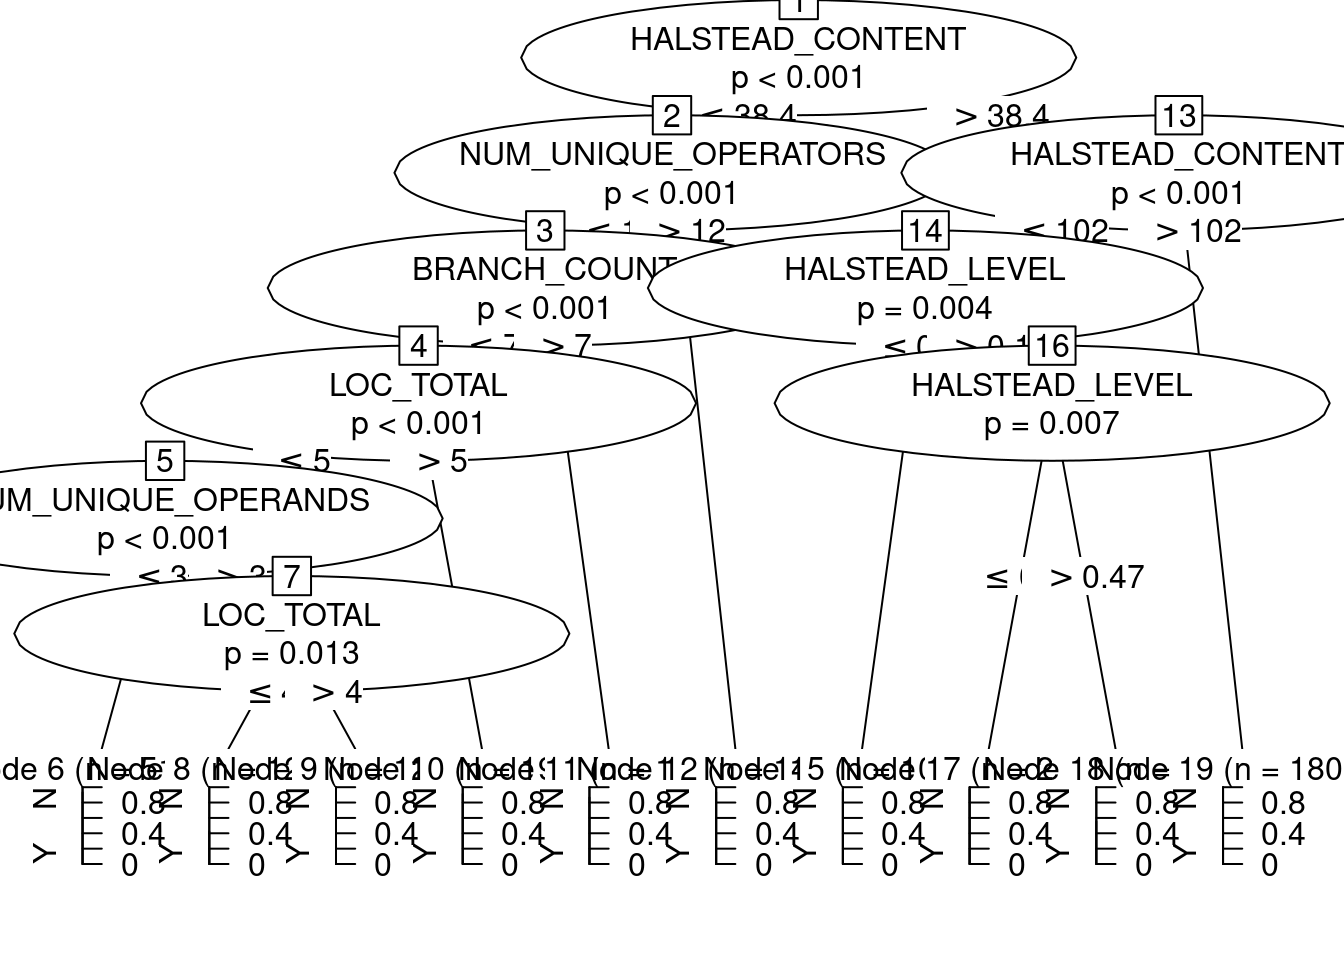
\includegraphics{DASE_files/figure-latex/unnamed-chunk-58-1.pdf} \\
Using the C50 package, there are two ways, specifying train and testing \\
\texttt{r\ library(C50)\ require(utils)\ \#\ c50t\ \textless{}-\ C5.0(jm1.train{[},-ncol(jm1.train){]},\ jm1.train{[},ncol(jm1.train){]})\ c50t\ \textless{}-\ C5.0(Defective\ \textasciitilde{}\ .,\ jm1.train)\ summary(c50t)\ plot(c50t)\ c50tPred\ \textless{}-\ predict(c50t,\ jm1.train)\ \#\ table(c50tPred,\ jm1.train\$Defective)} \\
Using the \href{https://cran.r-project.org/web/packages/rpart/index.html}{`rpart'} package \\
\texttt{r\ \#\ Using\ the\ \textquotesingle{}rpart\textquotesingle{}\ package\ library(rpart)\ jm1.rpart\ \textless{}-\ rpart(Defective\ \textasciitilde{}\ .,\ data=jm1.train,\ parms\ =\ list(prior\ =\ c(.65,.35),\ split\ =\ "information"))\ \#\ par(mfrow\ =\ c(1,2),\ xpd\ =\ NA)\ plot(jm1.rpart)\ text(jm1.rpart,\ use.n\ =\ TRUE)} \\
\includegraphics{DASE_files/figure-latex/unnamed-chunk-60-1.pdf} \\
\texttt{r\ jm1.rpart} \\
\texttt{\#\#\ n=\ 5757\ \#\#\ \#\#\ node),\ split,\ n,\ loss,\ yval,\ (yprob)\ \#\#\ \ \ \ \ \ \ *\ denotes\ terminal\ node\ \#\#\ \#\#\ \ 1)\ root\ 5757\ 2010.0\ N\ (0.650\ 0.350)\ \#\#\ \ \ \ 2)\ LOC\_TOTAL\textless{}\ 38.5\ 4172\ \ 969.0\ N\ (0.751\ 0.249)\ *\ \#\#\ \ \ \ 3)\ LOC\_TOTAL\textgreater{}=38.5\ 1585\ \ 825.0\ Y\ (0.441\ 0.559)\ \#\#\ \ \ \ \ \ 6)\ LOC\_TOTAL\textless{}\ 87.5\ 1027\ \ 540.0\ N\ (0.523\ 0.477)\ \#\#\ \ \ \ \ \ \ 12)\ LOC\_BLANK\textless{}\ 7.5\ 580\ \ 263.0\ N\ (0.572\ 0.428)\ *\ \#\#\ \ \ \ \ \ \ 13)\ LOC\_BLANK\textgreater{}=7.5\ 447\ \ 240.0\ Y\ (0.465\ 0.535)\ \#\#\ \ \ \ \ \ \ \ \ 26)\ HALSTEAD\_DIFFICULTY\textgreater{}=34.9\ 62\ \ \ 15.3\ N\ (0.738\ 0.262)\ *\ \#\#\ \ \ \ \ \ \ \ \ 27)\ HALSTEAD\_DIFFICULTY\textless{}\ 34.9\ 385\ \ 197.0\ Y\ (0.430\ 0.570)\ *\ \#\#\ \ \ \ \ \ 7)\ LOC\_TOTAL\textgreater{}=87.5\ 558\ \ 233.0\ Y\ (0.316\ 0.684)\ *} \\
\texttt{r\ library(rpart.plot)\ \#\ asRules(jm1.rpart)\ \#\ fancyRpartPlot(jm1.rpart)} \\
\#\# Rules \\
C5 Rules \\
\texttt{r\ library(C50)\ c50r\ \textless{}-\ C5.0(jm1.train{[},-ncol(jm1.train){]},\ jm1.train{[},ncol(jm1.train){]},\ rules\ =\ TRUE)\ summary(c50r)} \\
\texttt{\#\#\ \#\#\ Call:\ \#\#\ C5.0.default(x\ =\ jm1.train{[},\ -ncol(jm1.train){]},\ y\ =\ \#\#\ \ jm1.train{[},\ ncol(jm1.train){]},\ rules\ =\ TRUE)\ \#\#\ \#\#\ \#\#\ C5.0\ {[}Release\ 2.07\ GPL\ Edition{]}\ \ \ \ \ \ Sun\ Oct\ 10\ 13:35:54\ 2021\ \#\#\ -\/-\/-\/-\/-\/-\/-\/-\/-\/-\/-\/-\/-\/-\/-\/-\/-\/-\/-\/-\/-\/-\/-\/-\/-\/-\/-\/-\/-\/-\/-\ \#\#\ \#\#\ Class\ specified\ by\ attribute\ \textasciigrave{}outcome\textquotesingle{}\ \#\#\ \#\#\ Read\ 5757\ cases\ (22\ attributes)\ from\ undefined.data\ \#\#\ \#\#\ Rules:\ \#\#\ \#\#\ Rule\ 1:\ (5682/1005,\ lift\ 1.0)\ \#\#\ \ NUM\_OPERANDS\ \textless{}=\ 376\ \#\#\ \ -\textgreater{}\ \ class\ N\ \ {[}0.823{]}\ \#\#\ \#\#\ Rule\ 2:\ (75/24,\ lift\ 3.7)\ \#\#\ \ NUM\_OPERANDS\ \textgreater{}\ 376\ \#\#\ \ -\textgreater{}\ \ class\ Y\ \ {[}0.675{]}\ \#\#\ \#\#\ Default\ class:\ N\ \#\#\ \#\#\ \#\#\ Evaluation\ on\ training\ data\ (5757\ cases):\ \#\#\ \#\#\ \ \ \ \ \ \ \ \ \ Rules\ \#\#\ \ \ \ -\/-\/-\/-\/-\/-\/-\/-\/-\/-\/-\/-\/-\/-\/-\/-\ \#\#\ \ \ \ \ \ No\ \ \ \ \ \ Errors\ \#\#\ \#\#\ \ \ \ \ \ \ 2\ 1029(17.9\%)\ \ \ \textless{}\textless{}\ \#\#\ \#\#\ \#\#\ \ \ \ \ (a)\ \ \ (b)\ \ \ \ \textless{}-classified\ as\ \#\#\ \ \ \ -\/-\/-\/-\ \ -\/-\/-\/-\ \#\#\ \ \ \ 4677\ \ \ \ 24\ \ \ \ (a):\ class\ N\ \#\#\ \ \ \ 1005\ \ \ \ 51\ \ \ \ (b):\ class\ Y\ \#\#\ \#\#\ \#\#\ \ Attribute\ usage:\ \#\#\ \#\#\ \ 100.00\%\ NUM\_OPERANDS\ \#\#\ \#\#\ \#\#\ Time:\ 0.2\ secs} \\
\texttt{r\ \#\ c50rPred\ \textless{}-\ predict(c50r,\ jm1.train)\ \#\ table(c50rPred,\ jm1.train\$Defective)} \\
\#\# Distanced-based Methods \\
In this case, there is no model as such. Given a new instance to classify, this approach finds the closest \(k\)-neighbours to the given instance. \\
\includegraphics{./figures/279px-KnnClassification.svg.png}
(Source: Wikipedia - \url{https://en.wikipedia.org/wiki/K-nearest_neighbors_algorithm}) \\
```r
library(class)
m1 \textless- knn(train=jm1.train{[},-22{]}, test=jm1.test{[},-22{]}, cl=jm1.train{[},22{]}, k=3) \\
table(jm1.test{[},22{]},m1)
``` \\
\texttt{\#\#\ \ \ \ m1\ \#\#\ \ \ \ \ \ \ \ N\ \ \ \ Y\ \#\#\ \ \ N\ 2851\ \ 282\ \#\#\ \ \ Y\ \ 554\ \ 149} \\
\#\# Neural Networks \\
\includegraphics{./figures/neuralnet.png} \\
\includegraphics{./figures/neuralnet2.png} \\
\#\# Support Vector Machine \\
\includegraphics{./figures/Kernel_Machine.svg.png}
(Source: wikipedia \url{https://en.wikipedia.org/wiki/Support_vector_machine}) \\
\#\# Probabilistic Methods \\
\#\#\# Naive Bayes \\
Probabilistic graphical model assigning a probability to each possible outcome \(p(C_k, x_1,\ldots,x_n)\) \\
\includegraphics{./figures/classifier_NB.png} \\
Using the \texttt{klaR} package with \texttt{caret}: \\
\texttt{r\ library(caret)\ library(klaR)} \\
\texttt{\#\#\ Loading\ required\ package:\ MASS} \\
\texttt{\#\#\ \#\#\ Attaching\ package:\ \textquotesingle{}MASS\textquotesingle{}} \\
\texttt{\#\#\ The\ following\ object\ is\ masked\ from\ \textquotesingle{}package:dplyr\textquotesingle{}:\ \#\#\ \#\#\ \ \ \ \ select} \\
\texttt{\#\#\ The\ following\ object\ is\ masked\ from\ \textquotesingle{}package:sm\textquotesingle{}:\ \#\#\ \#\#\ \ \ \ \ muscle} \\
\texttt{r\ model\ \textless{}-\ NaiveBayes(Defective\ \textasciitilde{}\ .,\ data\ =\ jm1.train)\ predictions\ \textless{}-\ predict(model,\ jm1.test{[},-22{]})\ confusionMatrix(predictions\$class,\ jm1.test\$Defective)} \\
\texttt{\#\#\ Confusion\ Matrix\ and\ Statistics\ \#\#\ \#\#\ \ \ \ \ \ \ \ \ \ \ Reference\ \#\#\ Prediction\ \ \ \ N\ \ \ \ Y\ \#\#\ \ \ \ \ \ \ \ \ \ N\ 2963\ \ 554\ \#\#\ \ \ \ \ \ \ \ \ \ Y\ \ 170\ \ 149\ \#\#\ \#\#\ \ \ \ \ \ \ \ \ \ \ \ \ \ \ \ Accuracy\ :\ 0.811\ \#\#\ \ \ \ \ \ \ \ \ \ \ \ \ \ \ \ \ \ 95\%\ CI\ :\ (0.799,\ 0.824)\ \#\#\ \ \ \ \ No\ Information\ Rate\ :\ 0.817\ \#\#\ \ \ \ \ P-Value\ {[}Acc\ \textgreater{}\ NIR{]}\ :\ 0.815\ \#\#\ \#\#\ \ \ \ \ \ \ \ \ \ \ \ \ \ \ \ \ \ \ Kappa\ :\ 0.2\ \#\#\ \#\#\ \ Mcnemar\textquotesingle{}s\ Test\ P-Value\ :\ \textless{}2e-16\ \#\#\ \#\#\ \ \ \ \ \ \ \ \ \ \ \ \ Sensitivity\ :\ 0.946\ \#\#\ \ \ \ \ \ \ \ \ \ \ \ \ Specificity\ :\ 0.212\ \#\#\ \ \ \ \ \ \ \ \ \ Pos\ Pred\ Value\ :\ 0.842\ \#\#\ \ \ \ \ \ \ \ \ \ Neg\ Pred\ Value\ :\ 0.467\ \#\#\ \ \ \ \ \ \ \ \ \ \ \ \ \ Prevalence\ :\ 0.817\ \#\#\ \ \ \ \ \ \ \ \ \ Detection\ Rate\ :\ 0.772\ \#\#\ \ \ \ Detection\ Prevalence\ :\ 0.917\ \#\#\ \ \ \ \ \ \ Balanced\ Accuracy\ :\ 0.579\ \#\#\ \#\#\ \ \ \ \ \ \ \ \textquotesingle{}Positive\textquotesingle{}\ Class\ :\ N\ \#\#} \\
Using the \texttt{e1071} package: \\
```r
library (e1071)
n1 \textless-naiveBayes(jm1.train\$Defective \textasciitilde{} ., data=jm1.train) \\
\# Show first 3 results using `class'
head(predict(n1,jm1.test, type = c(``class'')),3) \# class by default
``` \\
\texttt{\#\#\ {[}1{]}\ Y\ Y\ Y\ \#\#\ Levels:\ N\ Y} \\
\texttt{r\ \#\ Show\ first\ 3\ results\ using\ \textquotesingle{}raw\textquotesingle{}\ head(predict(n1,jm1.test,\ type\ =\ c("raw")),3)} \\
\texttt{\#\#\ \ \ \ \ \ \ \ \ \ \ \ N\ Y\ \#\#\ {[}1,{]}\ 8.6e-50\ 1\ \#\#\ {[}2,{]}\ 0.0e+00\ 1\ \#\#\ {[}3,{]}\ 0.0e+00\ 1} \\
There are other variants such as TAN and KDB that do not assume the independece condition allowin us more complex structures. \\
\includegraphics{./figures/classifier_TAN.png} \\
\includegraphics{./figures/classifier_KDB.png} \\
A comprehensice comparison of \\
\#\# Linear Discriminant Analysis (LDA) \\
One classical approach to classification is Linear Discriminant Analysis (LDA), a generalization of Fisher's linear discriminant, as a method used to find a linear combination of features to separate two or more classes. \\
\texttt{r\ ldaModel\ \textless{}-\ train\ (Defective\ \textasciitilde{}\ .,\ data=jm1.train,\ method="lda",\ preProc=c("center","scale"))\ ldaModel} \\
\texttt{\#\#\ Linear\ Discriminant\ Analysis\ \#\#\ \#\#\ 5757\ samples\ \#\#\ \ \ 21\ predictor\ \#\#\ \ \ \ 2\ classes:\ \textquotesingle{}N\textquotesingle{},\ \textquotesingle{}Y\textquotesingle{}\ \#\#\ \#\#\ Pre-processing:\ centered\ (21),\ scaled\ (21)\ \#\#\ Resampling:\ Bootstrapped\ (25\ reps)\ \#\#\ Summary\ of\ sample\ sizes:\ 5757,\ 5757,\ 5757,\ 5757,\ 5757,\ 5757,\ ...\ \#\#\ Resampling\ results:\ \#\#\ \#\#\ \ \ Accuracy\ \ Kappa\ \#\#\ \ \ 0.82\ \ \ \ \ \ 0.164} \\
We can observe that we are training our model using \texttt{Defective\ \textasciitilde{}\ .} as a formula were \texttt{Defective} is the class variable separed by \texttt{\textasciitilde{}} and the ´.´ means the rest of the variables. Also, we are using a filter for the training data to (preProc) to center and scale. \\
Also, as stated in the documentation about the \texttt{train} method :
\textgreater{} \url{http://topepo.github.io/caret/training.html} \\
```r
ctrl \textless- trainControl(method = ``repeatedcv'',repeats=3)
ldaModel \textless- train (Defective \textasciitilde{} ., data=jm1.train, method=``lda'', trControl=ctrl, preProc=c(``center'',``scale'')) \\
ldaModel
``` \\
\texttt{\#\#\ Linear\ Discriminant\ Analysis\ \#\#\ \#\#\ 5757\ samples\ \#\#\ \ \ 21\ predictor\ \#\#\ \ \ \ 2\ classes:\ \textquotesingle{}N\textquotesingle{},\ \textquotesingle{}Y\textquotesingle{}\ \#\#\ \#\#\ Pre-processing:\ centered\ (21),\ scaled\ (21)\ \#\#\ Resampling:\ Cross-Validated\ (10\ fold,\ repeated\ 3\ times)\ \#\#\ Summary\ of\ sample\ sizes:\ 5181,\ 5182,\ 5181,\ 5182,\ 5180,\ 5181,\ ...\ \#\#\ Resampling\ results:\ \#\#\ \#\#\ \ \ Accuracy\ \ Kappa\ \#\#\ \ \ 0.82\ \ \ \ \ \ 0.159} \\
Instead of accuracy we can activate other metrics using \texttt{summaryFunction=twoClassSummary} such as \texttt{ROC}, \texttt{sensitivity} and \texttt{specificity}. To do so, we also need to speficy \texttt{classProbs=TRUE}. \\
```r
ctrl \textless- trainControl(method = ``repeatedcv'',repeats=3, classProbs=TRUE, summaryFunction=twoClassSummary)
ldaModel3xcv10 \textless- train (Defective \textasciitilde{} ., data=jm1.train, method=``lda'', trControl=ctrl, preProc=c(``center'',``scale'')) \\
ldaModel3xcv10
``` \\
\texttt{\#\#\ Linear\ Discriminant\ Analysis\ \#\#\ \#\#\ 5757\ samples\ \#\#\ \ \ 21\ predictor\ \#\#\ \ \ \ 2\ classes:\ \textquotesingle{}N\textquotesingle{},\ \textquotesingle{}Y\textquotesingle{}\ \#\#\ \#\#\ Pre-processing:\ centered\ (21),\ scaled\ (21)\ \#\#\ Resampling:\ Cross-Validated\ (10\ fold,\ repeated\ 3\ times)\ \#\#\ Summary\ of\ sample\ sizes:\ 5181,\ 5181,\ 5181,\ 5182,\ 5182,\ 5181,\ ...\ \#\#\ Resampling\ results:\ \#\#\ \#\#\ \ \ ROC\ \ \ \ Sens\ \ \ Spec\ \#\#\ \ \ 0.708\ \ 0.971\ \ 0.143} \\
Most methods have parameters that need to be optimised and that is one of the \\
```r
plsFit3x10cv \textless- train (Defective \textasciitilde{} ., data=jm1.train, method=``pls'', trControl=trainControl(classProbs=TRUE), metric=``ROC'', preProc=c(``center'',``scale'')) \\
plsFit3x10cv
``` \\
\texttt{\#\#\ Partial\ Least\ Squares\ \#\#\ \#\#\ 5757\ samples\ \#\#\ \ \ 21\ predictor\ \#\#\ \ \ \ 2\ classes:\ \textquotesingle{}N\textquotesingle{},\ \textquotesingle{}Y\textquotesingle{}\ \#\#\ \#\#\ Pre-processing:\ centered\ (21),\ scaled\ (21)\ \#\#\ Resampling:\ Bootstrapped\ (25\ reps)\ \#\#\ Summary\ of\ sample\ sizes:\ 5757,\ 5757,\ 5757,\ 5757,\ 5757,\ 5757,\ ...\ \#\#\ Resampling\ results\ across\ tuning\ parameters:\ \#\#\ \#\#\ \ \ ncomp\ \ Accuracy\ \ Kappa\ \#\#\ \ \ 1\ \ \ \ \ \ 0.821\ \ \ \ \ 0.0620\ \#\#\ \ \ 2\ \ \ \ \ \ 0.821\ \ \ \ \ 0.0978\ \#\#\ \ \ 3\ \ \ \ \ \ 0.821\ \ \ \ \ 0.0992\ \#\#\ \#\#\ Accuracy\ was\ used\ to\ select\ the\ optimal\ model\ using\ the\ largest\ value.\ \#\#\ The\ final\ value\ used\ for\ the\ model\ was\ ncomp\ =\ 3.} \\
\texttt{r\ plot(plsFit3x10cv)} \\
\includegraphics{DASE_files/figure-latex/unnamed-chunk-68-1.pdf} \\
The parameter \texttt{tuneLength} allow us to specify the number values per parameter to consider. \\
```r
plsFit3x10cv \textless- train (Defective \textasciitilde{} ., data=jm1.train, method=``pls'', trControl=ctrl, metric=``ROC'', tuneLength=5, preProc=c(``center'',``scale'')) \\
plsFit3x10cv
``` \\
\texttt{\#\#\ Partial\ Least\ Squares\ \#\#\ \#\#\ 5757\ samples\ \#\#\ \ \ 21\ predictor\ \#\#\ \ \ \ 2\ classes:\ \textquotesingle{}N\textquotesingle{},\ \textquotesingle{}Y\textquotesingle{}\ \#\#\ \#\#\ Pre-processing:\ centered\ (21),\ scaled\ (21)\ \#\#\ Resampling:\ Cross-Validated\ (10\ fold,\ repeated\ 3\ times)\ \#\#\ Summary\ of\ sample\ sizes:\ 5181,\ 5182,\ 5181,\ 5182,\ 5181,\ 5182,\ ...\ \#\#\ Resampling\ results\ across\ tuning\ parameters:\ \#\#\ \#\#\ \ \ ncomp\ \ ROC\ \ \ \ Sens\ \ \ Spec\ \#\#\ \ \ 1\ \ \ \ \ \ 0.700\ \ 0.996\ \ 0.0429\ \#\#\ \ \ 2\ \ \ \ \ \ 0.703\ \ 0.989\ \ 0.0710\ \#\#\ \ \ 3\ \ \ \ \ \ 0.706\ \ 0.990\ \ 0.0720\ \#\#\ \ \ 4\ \ \ \ \ \ 0.708\ \ 0.990\ \ 0.0808\ \#\#\ \ \ 5\ \ \ \ \ \ 0.708\ \ 0.990\ \ 0.0808\ \#\#\ \#\#\ ROC\ was\ used\ to\ select\ the\ optimal\ model\ using\ the\ largest\ value.\ \#\#\ The\ final\ value\ used\ for\ the\ model\ was\ ncomp\ =\ 5.} \\
\texttt{r\ plot(plsFit3x10cv)} \\
\includegraphics{DASE_files/figure-latex/unnamed-chunk-69-1.pdf} \\
Finally to predict new cases, \texttt{caret} will use the best classfier obtained for prediction. \\
\texttt{r\ plsProbs\ \textless{}-\ predict(plsFit3x10cv,\ newdata\ =\ jm1.test,\ type\ =\ "prob")} \\
\texttt{r\ plsClasses\ \textless{}-\ predict(plsFit3x10cv,\ newdata\ =\ jm1.test,\ type\ =\ "raw")\ confusionMatrix(data=plsClasses,jm1.test\$Defective)} \\
\texttt{\#\#\ Confusion\ Matrix\ and\ Statistics\ \#\#\ \#\#\ \ \ \ \ \ \ \ \ \ \ Reference\ \#\#\ Prediction\ \ \ \ N\ \ \ \ Y\ \#\#\ \ \ \ \ \ \ \ \ \ N\ 3094\ \ 652\ \#\#\ \ \ \ \ \ \ \ \ \ Y\ \ \ 39\ \ \ 51\ \#\#\ \#\#\ \ \ \ \ \ \ \ \ \ \ \ \ \ \ \ Accuracy\ :\ 0.82\ \#\#\ \ \ \ \ \ \ \ \ \ \ \ \ \ \ \ \ \ 95\%\ CI\ :\ (0.807,\ 0.832)\ \#\#\ \ \ \ \ No\ Information\ Rate\ :\ 0.817\ \#\#\ \ \ \ \ P-Value\ {[}Acc\ \textgreater{}\ NIR{]}\ :\ 0.317\ \#\#\ \#\#\ \ \ \ \ \ \ \ \ \ \ \ \ \ \ \ \ \ \ Kappa\ :\ 0.091\ \#\#\ \#\#\ \ Mcnemar\textquotesingle{}s\ Test\ P-Value\ :\ \textless{}2e-16\ \#\#\ \#\#\ \ \ \ \ \ \ \ \ \ \ \ \ Sensitivity\ :\ 0.9876\ \#\#\ \ \ \ \ \ \ \ \ \ \ \ \ Specificity\ :\ 0.0725\ \#\#\ \ \ \ \ \ \ \ \ \ Pos\ Pred\ Value\ :\ 0.8259\ \#\#\ \ \ \ \ \ \ \ \ \ Neg\ Pred\ Value\ :\ 0.5667\ \#\#\ \ \ \ \ \ \ \ \ \ \ \ \ \ Prevalence\ :\ 0.8167\ \#\#\ \ \ \ \ \ \ \ \ \ Detection\ Rate\ :\ 0.8066\ \#\#\ \ \ \ Detection\ Prevalence\ :\ 0.9765\ \#\#\ \ \ \ \ \ \ Balanced\ Accuracy\ :\ 0.5300\ \#\#\ \#\#\ \ \ \ \ \ \ \ \textquotesingle{}Positive\textquotesingle{}\ Class\ :\ N\ \#\#} \\
\#\#\# Predicting the number of defects (numerical class) \\
From the Bug Prediction Repository (BPR) \url{http://bug.inf.usi.ch/download.php} \\
Some datasets contain CK and other 11 object-oriented metrics for the last version of the system plus categorized (with severity and priority) post-release defects. Using such dataset: \\
```r
jdt \textless- read.csv(``./datasets/defectPred/BPD/single-version-ck-oo-EclipseJDTCore.csv'', sep=``;'') \\
\# We just use the number of bugs, so we removed others
jdt\(classname <- NULL jdt\)nonTrivialBugs \textless- NULL
jdt\(majorBugs <- NULL jdt\)minorBugs \textless- NULL
jdt\(criticalBugs <- NULL jdt\)highPriorityBugs \textless- NULL
jdt\$X \textless- NULL \\
\# Caret
library(caret) \\
\# Split data into training and test datasets
set.seed(1)
inTrain \textless- createDataPartition(y=jdt\$bugs,p=.8,list=FALSE)
jdt.train \textless- jdt{[}inTrain,{]}
jdt.test \textless- jdt{[}-inTrain,{]}
``` \\
\texttt{r\ ctrl\ \textless{}-\ trainControl(method\ =\ "repeatedcv",repeats=3)\ glmModel\ \textless{}-\ train\ (bugs\ \textasciitilde{}\ .,\ data=jdt.train,\ method="glm",\ trControl=ctrl,\ preProc=c("center","scale"))\ glmModel} \\
\texttt{\#\#\ Generalized\ Linear\ Model\ \#\#\ \#\#\ 798\ samples\ \#\#\ \ 17\ predictor\ \#\#\ \#\#\ Pre-processing:\ centered\ (17),\ scaled\ (17)\ \#\#\ Resampling:\ Cross-Validated\ (10\ fold,\ repeated\ 3\ times)\ \#\#\ Summary\ of\ sample\ sizes:\ 719,\ 718,\ 718,\ 718,\ 718,\ 718,\ ...\ \#\#\ Resampling\ results:\ \#\#\ \#\#\ \ \ RMSE\ \ \ Rsquared\ \ MAE\ \#\#\ \ \ 0.936\ \ 0.273\ \ \ \ \ 0.442} \\
Others such as Elasticnet: \\
\texttt{r\ glmnetModel\ \textless{}-\ train\ (bugs\ \textasciitilde{}\ .,\ data=jdt.train,\ method="glmnet",\ trControl=ctrl,\ preProc=c("center","scale"))\ glmnetModel} \\
\texttt{\#\#\ glmnet\ \#\#\ \#\#\ 798\ samples\ \#\#\ \ 17\ predictor\ \#\#\ \#\#\ Pre-processing:\ centered\ (17),\ scaled\ (17)\ \#\#\ Resampling:\ Cross-Validated\ (10\ fold,\ repeated\ 3\ times)\ \#\#\ Summary\ of\ sample\ sizes:\ 718,\ 718,\ 718,\ 718,\ 718,\ 718,\ ...\ \#\#\ Resampling\ results\ across\ tuning\ parameters:\ \#\#\ \#\#\ \ \ alpha\ \ lambda\ \ \ RMSE\ \ \ Rsquared\ \ MAE\ \#\#\ \ \ 0.10\ \ \ 0.00112\ \ 1.004\ \ 0.249\ \ \ \ \ 0.458\ \#\#\ \ \ 0.10\ \ \ 0.01120\ \ 0.938\ \ 0.247\ \ \ \ \ 0.447\ \#\#\ \ \ 0.10\ \ \ 0.11195\ \ 0.840\ \ 0.272\ \ \ \ \ 0.430\ \#\#\ \ \ 0.55\ \ \ 0.00112\ \ 1.006\ \ 0.249\ \ \ \ \ 0.458\ \#\#\ \ \ 0.55\ \ \ 0.01120\ \ 0.918\ \ 0.249\ \ \ \ \ 0.444\ \#\#\ \ \ 0.55\ \ \ 0.11195\ \ 0.825\ \ 0.286\ \ \ \ \ 0.433\ \#\#\ \ \ 1.00\ \ \ 0.00112\ \ 1.008\ \ 0.248\ \ \ \ \ 0.458\ \#\#\ \ \ 1.00\ \ \ 0.01120\ \ 0.902\ \ 0.252\ \ \ \ \ 0.442\ \#\#\ \ \ 1.00\ \ \ 0.11195\ \ 0.831\ \ 0.282\ \ \ \ \ 0.446\ \#\#\ \#\#\ RMSE\ was\ used\ to\ select\ the\ optimal\ model\ using\ the\ smallest\ value.\ \#\#\ The\ final\ values\ used\ for\ the\ model\ were\ alpha\ =\ 0.55\ and\ lambda\ =\ 0.112.} \\
\#\# Binary Logistic Regression (BLR) \\
Binary Logistic Regression (BLR) can models fault-proneness as follows \\
\(fp(X) = \frac{e^{logit()}}{1 + e^{logit(X)}}\) \\
where the simplest form for logit is: \\
\(logit(X) = c_{0} + c_{1}X\) \\
```r
jdt \textless- read.csv(``./datasets/defectPred/BPD/single-version-ck-oo-EclipseJDTCore.csv'', sep=``;'') \\
\# Caret
library(caret) \\
\# Convert the response variable into a boolean variable (0/1)
jdt\(bugs[jdt\)bugs\textgreater=1{]}\textless-1 \\
cbo \textless- jdt\(cbo bugs <- jdt\)bugs \\
\# Split data into training and test datasets
jdt2 = data.frame(cbo, bugs)
inTrain \textless- createDataPartition(y=jdt2\$bugs,p=.8,list=FALSE)
jdtTrain \textless- jdt2{[}inTrain,{]}
jdtTest \textless- jdt2{[}-inTrain,{]}
``` \\
BLR models fault-proneness are as follows \(fp(X) = \frac{e^{logit()}}{1 + e^{logit(X)}}\) \\
where the simplest form for logit is \(logit(X) = c_{0} + c_{1}X\) \\
```r
\# logit regression
\# glmLogit \textless- train (bugs \textasciitilde{} ., data=jdt.train, method=``glm'', family=binomial(link = logit)) \\
glmLogit \textless- glm (bugs \textasciitilde{} ., data=jdtTrain, family=binomial(link = logit))
summary(glmLogit)
``` \\
\texttt{\#\#\ \#\#\ Call:\ \#\#\ glm(formula\ =\ bugs\ \textasciitilde{}\ .,\ family\ =\ binomial(link\ =\ logit),\ data\ =\ jdtTrain)\ \#\#\ \#\#\ Deviance\ Residuals:\ \#\#\ \ \ \ Min\ \ \ \ \ \ 1Q\ \ Median\ \ \ \ \ \ 3Q\ \ \ \ \ Max\ \#\#\ -3.654\ \ -0.591\ \ -0.515\ \ -0.471\ \ \ 2.150\ \#\#\ \#\#\ Coefficients:\ \#\#\ \ \ \ \ \ \ \ \ \ \ \ \ Estimate\ Std.\ Error\ z\ value\ Pr(\textgreater{}\textbar{}z\textbar{})\ \#\#\ (Intercept)\ -2.20649\ \ \ \ 0.13900\ \ -15.87\ \ \ \textless{}2e-16\ ***\ \#\#\ cbo\ \ \ \ \ \ \ \ \ \ 0.06298\ \ \ \ 0.00765\ \ \ \ 8.23\ \ \ \textless{}2e-16\ ***\ \#\#\ -\/-\/-\ \#\#\ Signif.\ codes:\ \ 0\ \textquotesingle{}***\textquotesingle{}\ 0.001\ \textquotesingle{}**\textquotesingle{}\ 0.01\ \textquotesingle{}*\textquotesingle{}\ 0.05\ \textquotesingle{}.\textquotesingle{}\ 0.1\ \textquotesingle{}\ \textquotesingle{}\ 1\ \#\#\ \#\#\ (Dispersion\ parameter\ for\ binomial\ family\ taken\ to\ be\ 1)\ \#\#\ \#\#\ \ \ \ \ Null\ deviance:\ 807.98\ \ on\ 797\ \ degrees\ of\ freedom\ \#\#\ Residual\ deviance:\ 691.80\ \ on\ 796\ \ degrees\ of\ freedom\ \#\#\ AIC:\ 695.8\ \#\#\ \#\#\ Number\ of\ Fisher\ Scoring\ iterations:\ 5} \\
Predict a single point: \\
\texttt{r\ newData\ =\ data.frame(cbo\ =\ 3)\ predict(glmLogit,\ newData,\ type\ =\ "response")} \\
\texttt{\#\#\ \ \ \ \ 1\ \#\#\ 0.117} \\
Draw the results, modified from:
\url{http://www.shizukalab.com/toolkits/plotting-logistic-regression-in-r} \\
```r
results \textless- predict(glmLogit, jdtTest, type = ``response'') \\
range(jdtTrain\$cbo)
``` \\
\texttt{\#\#\ {[}1{]}\ \ \ 0\ 156} \\
\texttt{r\ range(results)} \\
\texttt{\#\#\ {[}1{]}\ 0.0992\ 0.9993} \\
\texttt{r\ plot(jdt2\$cbo,jdt2\$bugs)\ curve(predict(glmLogit,\ data.frame(cbo=x),\ type\ =\ "response"),add=TRUE)} \\
\includegraphics{DASE_files/figure-latex/unnamed-chunk-78-1.pdf} \\
\texttt{r\ \#\ points(jdtTrain\$cbo,fitted(glmLogit))} \\
Another type of graph: \\
\texttt{r\ library(popbio)} \\
\texttt{\#\#\ \#\#\ Attaching\ package:\ \textquotesingle{}popbio\textquotesingle{}} \\
\texttt{\#\#\ The\ following\ object\ is\ masked\ from\ \textquotesingle{}package:caret\textquotesingle{}:\ \#\#\ \#\#\ \ \ \ \ sensitivity} \\
\texttt{r\ logi.hist.plot(jdt2\$cbo,jdt2\$bugs,boxp=FALSE,type="hist",col="gray")} \\
\includegraphics{DASE_files/figure-latex/unnamed-chunk-79-1.pdf} \\
\#\# The caret package \\
There are hundreds of packages to perform classification task in R, but many of those can be used throught the `caret' package which helps with many of the data mining process task as described next. \\
The caret package\url{http://topepo.github.io/caret/} provides a unified interface for modeling and prediction with around 150 different models with tools for: \\
+ data splitting \\
+ pre-processing \\
+ feature selection \\
+ model tuning using resampling \\
+ variable importance estimation, etc. \\
Website: \url{http://caret.r-forge.r-project.org} \\
JSS Paper: \url{www.jstatsoft.org/v28/i05/paper} \\
Book: \href{http://AppliedPredictiveModeling.com/}{Applied Predictive Modeling} \\
 \\
\# Regression \{\#regression\} \\
\#\# Linear Regression modeling \\
- \emph{Linear Regression} is one of the oldest and most known predictive methods. As its name says, the idea is to try to fit a linear equation between a dependent variable and an independent, or explanatory, variable. The idea is that the independent variable \(x\) is something the experimenter controls and the dependent variable \(y\) is something that the experimenter measures. The line is used to predict the value of \(y\) for a known value of \(x\). The variable \(x\) is the predictor variable and \(y\) the response variable. \\
- \emph{Multiple linear regression} uses 2 or more independent variables for building a model. See \url{https://www.wikipedia.org/wiki/Linear_regression}. \\
- First proposed many years ago but still very useful\ldots{} \\
\includegraphics{figures/galton.png} \\
- The equation takes the form \(\hat{y}=b_0+b_1 * x\)
- The method used to choose the values \(b_0\) and \(b_1\) is to minimize the sum of the squares of the residual errors. \\
\#\#\# Regression: Galton Data \\
Not related to Software Engineering but \ldots{} \\
\texttt{r\ library(UsingR)\ data(galton)\ par(mfrow=c(1,2))\ hist(galton\$child,col="blue",breaks=100)\ hist(galton\$parent,col="blue",breaks=100)} \\
\includegraphics{DASE_files/figure-latex/unnamed-chunk-80-1.pdf} \\
\texttt{r\ plot(galton\$parent,galton\$child,pch=1,col="blue",\ cex=0.4)\ lm1\ \textless{}-\ lm(galton\$child\ \textasciitilde{}\ galton\$parent)\ lines(galton\$parent,lm1\$fitted,col="red",lwd=3)\ plot(galton\$parent,lm1\$residuals,col="blue",pch=1,\ cex=0.4)\ abline(c(0,0),col="red",lwd=3)} \\
\includegraphics{DASE_files/figure-latex/unnamed-chunk-80-2.pdf} \\
\texttt{r\ qqnorm(galton\$child)} \\
\includegraphics{DASE_files/figure-latex/unnamed-chunk-80-3.pdf} \\
\#\#\# Simple Linear Regression \\
- Given two variables \(Y\) (response) and \(X\) (predictor), the assumption is that there is an approximate (\(\approx\)) \emph{linear} relation between those variables.
- The mathematical model of the observed data is described as (for the case of simple linear regression):
\( Y \approx \beta_0 + \beta_1 X\) \\
- the parameter \(\beta_0\) is named the \emph{intercept} and \(\beta_1\) is the \emph{slope}
- Each observation can be modeled as \\
\(y_i = \beta_0 + \beta_1 x_i + \epsilon_i;
\epsilon_i \sim N(0,\sigma^2)\)
- \(\epsilon_i\) is the \emph{error}
- This means that the variable \(y\) is normally distributed:
\( y_i \sim N( \beta_0 + \beta_1 x_i, \sigma^2) \) \\
- The \emph{predictions} or \emph{estimations} of this model are obtained by a linear equation of the form \(\hat{Y}=\hat{\beta_0} + \hat{\beta}_1X\), that is, each new prediction is computed with
\(\hat{y}_i = \hat{\beta}_0 + \hat{\beta}_1x_i \).
- The actual parameters \(\beta_0\) and \(\beta_1\) are unknown
- The parameters \(\hat{\beta}_0\) and \(\hat{\beta}_1\) of the linear equation can be estimated with different methods. \\
\#\#\# Least Squares \\
- One of the most used methods for computing \(\hat{\beta}_0\) and \(\hat{\beta}_1\) is the criterion of ``least squares'' minimization.
- The data is composed of \(n\) pairs of observations \((x_i, y_i)\)
- Given an observation \(y_i\) and its corresponding estimation \(\hat{y_i})\) the \emph{residual} \(e_i\) is defined as \(e_i= y_i - \hat{y_i}\)
- the Residual Sum of Squares is defined as \(RSS=e_1^2+\dots + e_i^2+\dots+e_n^2\)
- the Least Squares Approach minimizes the RSS
- as result of that minimizitation, it can be obtained, by means of calculus, the estimation of \(\hat{\beta}_0\) and \(\hat{\beta}_1\) as \(\hat{\beta}_1=\frac{\sum_{i=1}^{n}{(x_i-\bar{x})(y_i-\bar{y})}}{\sum_{i=1}^{n}(x_i-\bar{x})^2}\) and \(\hat{\beta}_0=\bar{y}-\hat{\beta}_1\bar{x} \) where \(\bar{y}\) and \(\bar{x}\) are the sample means.
- the variance \(\sigma^2\) is estimated by
\(\hat\sigma^2 = {RSS}/{(n-2)}\) where n is the number of observations
- The \emph{Residual Standard Error} is defined as \(RSE = \sqrt{{RSS}/{(n-2)}}\)
- The equation \( Y = \beta_0 + \beta_1 X + \epsilon\) defines the linear model, i.e., the \emph{population regression line}
- The \emph{least squares line} is \(\hat{Y}=\hat{\beta_0} + \hat{\beta}_1X\)
- \emph{Confidence intervals} are computed using the \emph{standard errors} of the intercept and the slope.
- The \(95\%\) confidence interval for the slope is computed as \([\hat{\beta}_1 - 2 \cdot SE(\hat{\beta}_1), \hat{\beta}_1+SE(\hat{\beta}_1)]\)
- where \( SE(\hat{\beta}_1) = \sqrt{\frac{\sigma^2}{\sum_{i=1}^{n}(x_i-\bar{x})^2}}\) \\
\#\#\# Linear regression in R \\
The following are the basic commands in R: \\
- The basic function is \texttt{lm()}, that returns an object with the model.
- Other commands: \texttt{summary} prints out information about the regression, \texttt{coef} gives the coefficients for the linear model, \texttt{fitted} gives the predictd value of \(y\) for each value of \(x\), \texttt{residuals} contains the differences between observed and fitted values.
- \href{https://stat.ethz.ch/R-manual/R-devel/library/stats/html/predict.lm.html}{\texttt{predict}} will generate predicted values of the response for the values of the explanatory variable. \\
\#\# Linear Regression Diagnostics \\
- Several plots help to evaluate the suitability of the linear regression
+ \emph{Residuals vs fitted}: The residuals should be randomly distributed around the horizontal line representing a residual error of zero; that is, there should not be a distinct trend in the distribution of points.
+ \emph{Standard Q-Q plot}: residual errors are normally distributed
+ \emph{Square root of the standardized residuals vs the fitted values}: there should be no obvious trend. This plot is similar to the residuals versus fitted values plot, but it uses the square root of the standardized residuals.
+ \emph{Leverage}: measures the importance of each point in determining the regression result. Smaller values means that removing the observation has little effect on the regression result. \\
\#\#\# Simulation example \\
\#\#\#\# Simulate a dataset \\
```r
set.seed(3456)
\# equation is y = -6.6 + 0.13 x +e
\# range x 100,400
a \textless- -6.6
b \textless- 0.13
num\_obs \textless- 60
xmin \textless- 100
xmax \textless- 400
x \textless- sample(seq(from=xmin, to = xmax, by =1), size= num\_obs, replace=FALSE) \\
sderror \textless- 9 \# sigma for the error term in the model
e \textless- rnorm(num\_obs, 0, sderror) \\
y \textless- a + b * x + e \\
newlm \textless- lm(y\textasciitilde x)
summary(newlm)
``` \\
\texttt{\#\#\ \#\#\ Call:\ \#\#\ lm(formula\ =\ y\ \textasciitilde{}\ x)\ \#\#\ \#\#\ Residuals:\ \#\#\ \ \ \ \ Min\ \ \ \ \ \ 1Q\ \ Median\ \ \ \ \ \ 3Q\ \ \ \ \ Max\ \#\#\ -26.518\ \ -5.645\ \ \ 0.363\ \ \ 5.695\ \ 18.392\ \#\#\ \#\#\ Coefficients:\ \#\#\ \ \ \ \ \ \ \ \ \ \ \ \ Estimate\ Std.\ Error\ t\ value\ Pr(\textgreater{}\textbar{}t\textbar{})\ \#\#\ (Intercept)\ \ -7.9060\ \ \ \ \ 3.3922\ \ \ -2.33\ \ \ \ 0.023\ *\ \#\#\ x\ \ \ \ \ \ \ \ \ \ \ \ \ 0.1331\ \ \ \ \ 0.0132\ \ \ 10.05\ \ 2.6e-14\ ***\ \#\#\ -\/-\/-\ \#\#\ Signif.\ codes:\ \ 0\ \textquotesingle{}***\textquotesingle{}\ 0.001\ \textquotesingle{}**\textquotesingle{}\ 0.01\ \textquotesingle{}*\textquotesingle{}\ 0.05\ \textquotesingle{}.\textquotesingle{}\ 0.1\ \textquotesingle{}\ \textquotesingle{}\ 1\ \#\#\ \#\#\ Residual\ standard\ error:\ 8.48\ on\ 58\ degrees\ of\ freedom\ \#\#\ Multiple\ R-squared:\ \ 0.635,\ \ Adjusted\ R-squared:\ \ 0.629\ \#\#\ F-statistic:\ \ 101\ on\ 1\ and\ 58\ DF,\ \ p-value:\ 2.57e-14} \\
```r
cfa1 \textless- coef(newlm){[}1{]}
cfb2 \textless- coef(newlm){[}2{]}
plot(x,y, xlab=``x axis'', ylab= ``y axis'', xlim = c(xmin, xmax), ylim = c(0,60), sub = ``Line in black is the actual model'')
title(main = paste(``Line in blue is the Regression Line for'', num\_obs, '' points.'')) \\
abline(a = cfa1, b = cfb2, col= ``blue'', lwd=3)
abline(a = a, b = b, col= ``black'', lwd=1) \#original line
``` \\
\includegraphics{DASE_files/figure-latex/unnamed-chunk-81-1.pdf} \\
\#\#\#\#\# Subset a set of points from the same sample \\
```r
\# sample from the same x to compare least squares lines
\# change the denominator in newsample to see how the least square lines changes accordingly.
newsample \textless- as.integer(num\_obs/8) \# number of pairs x,y \\
idxs\_x1 \textless- sample(1:num\_obs, size = newsample, replace = FALSE) \#sample indexes
x1 \textless- x{[}idxs\_x1{]}
e1 \textless- e{[}idxs\_x1{]}
y1 \textless- a + b * x1 + e1
xy\_obs \textless- data.frame(x1, y1)
names(xy\_obs) \textless- c(``x\_obs'', ``y\_obs'') \\
newlm1 \textless- lm(y1\textasciitilde x1)
summary(newlm1)
``` \\
\texttt{\#\#\ \#\#\ Call:\ \#\#\ lm(formula\ =\ y1\ \textasciitilde{}\ x1)\ \#\#\ \#\#\ Residuals:\ \#\#\ \ \ \ \ \ 1\ \ \ \ \ \ 2\ \ \ \ \ \ 3\ \ \ \ \ \ 4\ \ \ \ \ \ 5\ \ \ \ \ \ 6\ \ \ \ \ \ 7\ \#\#\ \ 3.968\ -8.537\ \ 3.141\ -8.723\ \ 7.294\ -0.235\ \ 3.092\ \#\#\ \#\#\ Coefficients:\ \#\#\ \ \ \ \ \ \ \ \ \ \ \ \ Estimate\ Std.\ Error\ t\ value\ Pr(\textgreater{}\textbar{}t\textbar{})\ \#\#\ (Intercept)\ \ \ 2.9107\ \ \ \ \ 7.7166\ \ \ \ 0.38\ \ \ \ 0.722\ \#\#\ x1\ \ \ \ \ \ \ \ \ \ \ \ 0.0913\ \ \ \ \ 0.0328\ \ \ \ 2.79\ \ \ \ 0.039\ *\ \#\#\ -\/-\/-\ \#\#\ Signif.\ codes:\ \ 0\ \textquotesingle{}***\textquotesingle{}\ 0.001\ \textquotesingle{}**\textquotesingle{}\ 0.01\ \textquotesingle{}*\textquotesingle{}\ 0.05\ \textquotesingle{}.\textquotesingle{}\ 0.1\ \textquotesingle{}\ \textquotesingle{}\ 1\ \#\#\ \#\#\ Residual\ standard\ error:\ 6.89\ on\ 5\ degrees\ of\ freedom\ \#\#\ Multiple\ R-squared:\ \ 0.609,\ \ Adjusted\ R-squared:\ \ 0.53\ \#\#\ F-statistic:\ 7.77\ on\ 1\ and\ 5\ DF,\ \ p-value:\ 0.0385} \\
```r
cfa21 \textless- coef(newlm1){[}1{]}
cfb22 \textless- coef(newlm1){[}2{]} \\
plot(x1,y1, xlab=``x axis'', ylab= ``y axis'', xlim = c(xmin, xmax), ylim = c(0,60))
title(main = paste(``New line in red with'', newsample, '' points in sample'')) \\
abline(a = a, b = b, col= ``black'', lwd=1) \# True line
abline(a = cfa1, b = cfb2, col= ``blue'', lwd=1) \#sample
abline(a = cfa21, b = cfb22, col= ``red'', lwd=2) \#new line
``` \\
\includegraphics{DASE_files/figure-latex/unnamed-chunk-82-1.pdf} \\
\#\#\#\#\# Compute a confidence interval on the original sample regression line \\
```r
newx \textless- seq(xmin, xmax)
ypredicted \textless- predict(newlm, newdata=data.frame(x=newx), interval= ``confidence'', level= 0.90, se = TRUE) \\
plot(x,y, xlab=``x axis'', ylab= ``y axis'', xlim = c(xmin, xmax), ylim = c(0,60))
\# points(x1, fitted(newlm1))
abline(newlm) \\
lines(newx,ypredicted\(fit[,2],col="red",lty=2) lines(newx,ypredicted\)fit{[},3{]},col=``red'',lty=2)
``` \\
\includegraphics{DASE_files/figure-latex/unnamed-chunk-83-1.pdf} \\
\texttt{r\ \#\ Plot\ the\ residuals\ or\ errors\ ypredicted\_x\ \textless{}-\ predict(newlm,\ newdata=data.frame(x=x))\ plot(x,y,\ xlab="x\ axis",\ ylab=\ "y\ axis",\ xlim\ =\ c(xmin,\ xmax),\ ylim\ =\ c(0,60),\ sub\ =\ "",\ pch=19,\ cex=0.75)\ title(main\ =\ paste("Residuals\ or\ errors",\ num\_obs,\ "\ points."))\ abline(newlm)\ segments(x,\ y,\ x,\ ypredicted\_x)} \\
\includegraphics{DASE_files/figure-latex/unnamed-chunk-83-2.pdf} \\
\#\#\#\#\# Take another sample from the model and explore \\
```r
\# equation is y = -6.6 + 0.13 x +e
\# range x 100,400
num\_obs \textless- 35
xmin \textless- 100
xmax \textless- 400
x3 \textless- sample(seq(from=xmin, to = xmax, by =1), size= num\_obs, replace=FALSE)
sderror \textless- 14 \# sigma for the error term in the model
e3 \textless- rnorm(num\_obs, 0, sderror) \\
y3 \textless- a + b * x3 + e3 \\
newlm3 \textless- lm(y3\textasciitilde x3)
summary(newlm3)
``` \\
\texttt{\#\#\ \#\#\ Call:\ \#\#\ lm(formula\ =\ y3\ \textasciitilde{}\ x3)\ \#\#\ \#\#\ Residuals:\ \#\#\ \ \ \ Min\ \ \ \ \ 1Q\ Median\ \ \ \ \ 3Q\ \ \ \ Max\ \#\#\ -40.87\ \ -9.20\ \ -2.28\ \ 12.08\ \ 47.17\ \#\#\ \#\#\ Coefficients:\ \#\#\ \ \ \ \ \ \ \ \ \ \ \ \ Estimate\ Std.\ Error\ t\ value\ Pr(\textgreater{}\textbar{}t\textbar{})\ \#\#\ (Intercept)\ \ -0.9284\ \ \ \ \ 8.7458\ \ \ -0.11\ \ \ 0.9161\ \#\#\ x3\ \ \ \ \ \ \ \ \ \ \ \ 0.1193\ \ \ \ \ 0.0345\ \ \ \ 3.45\ \ \ 0.0015\ **\ \#\#\ -\/-\/-\ \#\#\ Signif.\ codes:\ \ 0\ \textquotesingle{}***\textquotesingle{}\ 0.001\ \textquotesingle{}**\textquotesingle{}\ 0.01\ \textquotesingle{}*\textquotesingle{}\ 0.05\ \textquotesingle{}.\textquotesingle{}\ 0.1\ \textquotesingle{}\ \textquotesingle{}\ 1\ \#\#\ \#\#\ Residual\ standard\ error:\ 17.2\ on\ 33\ degrees\ of\ freedom\ \#\#\ Multiple\ R-squared:\ \ 0.266,\ \ Adjusted\ R-squared:\ \ 0.243\ \#\#\ F-statistic:\ 11.9\ on\ 1\ and\ 33\ DF,\ \ p-value:\ 0.00153} \\
```r
cfa31 \textless- coef(newlm3){[}1{]}
cfb32 \textless- coef(newlm3){[}2{]}
plot(x3,y3, xlab=``x axis'', ylab= ``y axis'', xlim = c(xmin, xmax), ylim = c(0,60))
title(main = paste(``Line in red is the Regression Line for'', num\_obs, '' points.''))
abline(a = cfa31, b = cfb32, col= ``red'', lwd=3)
abline(a = a, b = b, col= ``black'', lwd=2) \#original line
abline(a = cfa1, b = cfb2, col= ``blue'', lwd=1) \#first sample \\
\# confidence intervals for the new sample \\
newx \textless- seq(xmin, xmax)
ypredicted \textless- predict(newlm3, newdata=data.frame(x3=newx), interval= ``confidence'', level= 0.90, se = TRUE) \\
lines(newx,ypredicted\(fit[,2],col="red",lty=2, lwd=2) lines(newx,ypredicted\)fit{[},3{]},col=``red'',lty=2, lwd=2)
``` \\
\includegraphics{DASE_files/figure-latex/unnamed-chunk-84-1.pdf} \\
\#\#\# Diagnostics fro assessing the regression line \\
\#\#\#\# Residual Standard Error
- It gives us an idea of the typical or average error of the model. It is the estimated standard deviation of the residuals. \\
\#\#\#\# \(R^2\) statistic
- This is the proportion of variability in the data that is explained by the model. Best values are those close to 1. \\
\#\# Multiple Linear Regression \\
\#\#\# Partial Least Squares
- If several predictors are highly correlated, the least squares approach has high variability.
- PLS finds linear combinations of the predictors, that are called \emph{components} or \emph{latent} variables. \\
\#\# Linear regression in Software Effort estimation \\
Fitting a linear model to log-log
- the predictive power equation is \(y= e^{b_0}*x^{b_1}\), ignoring the bias corrections. Note: depending how the error term behaves we could try another general linear model (GLM) or other model that does not rely on the normality of the residuals (quantile regression, etc.)
- First, we are fitting the model to the whole dataset. But it is not the right way to do it, because of overfitting. \\
\texttt{r\ library(foreign)\ china\ \textless{}-\ read.arff("./datasets/effortEstimation/china.arff")\ china\_size\ \textless{}-\ china\$AFP\ summary(china\_size)} \\
\texttt{\#\#\ \ \ \ Min.\ 1st\ Qu.\ \ Median\ \ \ \ Mean\ 3rd\ Qu.\ \ \ \ Max.\ \#\#\ \ \ \ \ \ \ 9\ \ \ \ \ 100\ \ \ \ \ 215\ \ \ \ \ 487\ \ \ \ \ 438\ \ \ 17518} \\
\texttt{r\ china\_effort\ \textless{}-\ china\$Effort\ summary(china\_effort)} \\
\texttt{\#\#\ \ \ \ Min.\ 1st\ Qu.\ \ Median\ \ \ \ Mean\ 3rd\ Qu.\ \ \ \ Max.\ \#\#\ \ \ \ \ \ 26\ \ \ \ \ 704\ \ \ \ 1829\ \ \ \ 3921\ \ \ \ 3826\ \ \ 54620} \\
\texttt{r\ par(mfrow=c(1,2))\ hist(china\_size,\ col="blue",\ xlab="Adjusted\ Function\ Points",\ main="Distribution\ of\ AFP")\ hist(china\_effort,\ col="blue",xlab="Effort",\ main="Distribution\ of\ Effort")} \\
\includegraphics{DASE_files/figure-latex/unnamed-chunk-85-1.pdf} \\
\texttt{r\ boxplot(china\_size)\ boxplot(china\_effort)} \\
\includegraphics{DASE_files/figure-latex/unnamed-chunk-85-2.pdf} \\
\texttt{r\ qqnorm(china\_size)\ qqline(china\_size)\ qqnorm(china\_effort)\ qqline(china\_effort)} \\
\includegraphics{DASE_files/figure-latex/unnamed-chunk-85-3.pdf} \\
Applying the \texttt{log} function (it computes natural logarithms, base \(e\)) \\
\includegraphics{DASE_files/figure-latex/unnamed-chunk-86-1.pdf} \includegraphics{DASE_files/figure-latex/unnamed-chunk-86-2.pdf} \\
\texttt{r\ linmodel\_logchina\ \textless{}-\ lm(logchina\_effort\ \textasciitilde{}\ logchina\_size)\ par(mfrow=c(1,1))\ plot(logchina\_size,\ logchina\_effort)\ abline(linmodel\_logchina,\ lwd=3,\ col=3)} \\
\includegraphics{DASE_files/figure-latex/unnamed-chunk-87-1.pdf} \\
\texttt{r\ par(mfrow=c(1,2))\ plot(linmodel\_logchina,\ ask\ =\ FALSE)} \\
\includegraphics{DASE_files/figure-latex/unnamed-chunk-87-2.pdf} \includegraphics{DASE_files/figure-latex/unnamed-chunk-87-3.pdf} \\
\texttt{r\ linmodel\_logchina} \\
\texttt{\#\#\ \#\#\ Call:\ \#\#\ lm(formula\ =\ logchina\_effort\ \textasciitilde{}\ logchina\_size)\ \#\#\ \#\#\ Coefficients:\ \#\#\ \ \ (Intercept)\ \ logchina\_size\ \#\#\ \ \ \ \ \ \ \ \ 3.301\ \ \ \ \ \ \ \ \ \ 0.768} \\
\#\# References \\
- The New Statistics with R, Andy Hector, 2015
- An Introduction to R, W.N. Venables and D.M. Smith and the R Development Core Team
- Practical Data Science with R, Nina Zumel and John Mount
- G. James et al, An Introduction to Statistical Learning with Applications in R, Springer, 2013 \\
 \\
\# (PART) Unsupervised Models \{-\} \\
\# Unsupervised or Descriptive modeling \\
From the descriptive (unsupervised) point of view, patterns are found to predict future behaviour or estimate. This include association rules, clustering, or tree clustering which aim at grouping together objects (e.g., animals) into successively larger clusters, using some measure of similarity or distance. The dataset will be as the previous table without the \(C\) class attribute \\
\textbar{} Att\textsubscript{1}\textbar{} \textbar{} Att\textsubscript{n} \textbar{}
\textbar-------\textbar-----\textbar{} -------\textbar{}
\textbar{} a\textsubscript{11} \textbar{} \ldots{} \textbar{} a\textsubscript{1n} \textbar{}
\textbar{} a\textsubscript{21} \textbar{} \ldots{} \textbar{} a\textsubscript{2n} \textbar{}
\textbar{} \ldots{} \textbar{} \ldots{} \textbar{} \ldots{} \textbar{}
\textbar{} a\textsubscript{m1} \textbar{} \ldots{} \textbar{} a\textsubscript{mn} \textbar{} \\
\#\# Clustering \\
```r
library(foreign)
library(fpc) \\
kc1 \textless- read.arff(``./datasets/defectPred/D1/KC1.arff'') \\
\# Split into training and test datasets
set.seed(1)
ind \textless- sample(2, nrow(kc1), replace = TRUE, prob = c(0.7, 0.3))
kc1.train \textless- kc1{[}ind==1, {]}
kc1.test \textless- kc1{[}ind==2, {]} \\
\# No class
kc1.train\$Defective \textless- NULL \\
ds \textless- dbscan(kc1.train, eps = 0.42, MinPts = 5) \\
kc1.kmeans \textless- kmeans(kc1.train, 2)
``` \\
\#\#\# k-Means \\
\texttt{r\ library(reshape,\ quietly=TRUE)\ library(graphics)\ kc1kmeans\ \textless{}-\ kmeans(sapply(na.omit(kc1.train),\ rescaler,\ "range"),\ 10)\ \#plot(kc1kmeans,\ col\ =\ kc1kmeans\$cluster)\ \#points(kc1kmeans\$centers,\ col\ =\ 1:5,\ pch\ =\ 8)} \\
\#\# Association rules \\
```r
library(arules) \\
\# x \textless- as.numeric(kc1\$LOC\_TOTAL)
\# str(x)
\# summary(x)
\# hist(x, breaks=30, main=``LoC Total'')
\# xDisc \textless- discretize(x, categories=5)
\# table(xDisc) \\
for(i in 1:21) kc1{[},i{]} \textless- discretize(kc1{[},i{]}, method = ``interval'', breaks = 5) \\
rules \textless- apriori(kc1,
parameter = list(minlen=3, supp=0.05, conf=0.35),
appearance = list(rhs=c(``Defective=Y''),
default=``lhs''),
control = list(verbose=F)) \\
\#rules \textless- apriori(kc1,
\# parameter = list(minlen=2, supp=0.05, conf=0.3),
\# appearance = list(rhs=c(``Defective=Y'', ``Defective=N''),
\# default=``lhs'')) \\
inspect(rules)
``` \\
\texttt{\#\#\ \ \ \ \ lhs\ \ \ \ \ \ \ \ \ \ \ \ \ \ \ \ \ \ \ \ \ \ \ \ \ \ \ \ \ \ \ rhs\ \ \ \ \ \ \ \ \ \ \ support\ confidence\ coverage\ lift\ count\ \#\#\ {[}1{]}\ \{HALSTEAD\_CONTENT={[}38.6,77.2),\ \#\#\ \ \ \ \ \ HALSTEAD\_LEVEL={[}0,0.4)\}\ \ \ \ \ \ \ =\textgreater{}\ \{Defective=Y\}\ \ 0.0539\ \ \ \ \ \ 0.370\ \ \ \ 0.146\ 2.39\ \ \ 113\ \#\#\ {[}2{]}\ \{LOC\_CODE\_AND\_COMMENT={[}0,2.4),\ \#\#\ \ \ \ \ \ HALSTEAD\_CONTENT={[}38.6,77.2)\}\ =\textgreater{}\ \{Defective=Y\}\ \ 0.0525\ \ \ \ \ \ 0.377\ \ \ \ 0.139\ 2.43\ \ \ 110\ \#\#\ {[}3{]}\ \{LOC\_CODE\_AND\_COMMENT={[}0,2.4),\ \#\#\ \ \ \ \ \ HALSTEAD\_CONTENT={[}38.6,77.2),\ \#\#\ \ \ \ \ \ HALSTEAD\_LEVEL={[}0,0.4)\}\ \ \ \ \ \ \ =\textgreater{}\ \{Defective=Y\}\ \ 0.0515\ \ \ \ \ \ 0.374\ \ \ \ 0.138\ 2.41\ \ \ 108} \\
\texttt{r\ library(arulesViz)\ plot(rules)} \\
\includegraphics{DASE_files/figure-latex/unnamed-chunk-90-1.pdf} \\
 \\
\# (PART) Evaluation \{-\} \\
\# Evaluation of Models \\
Once we obtain the model with the training data, we need to evaluate it with some new data (testing data). \\
\textgreater{} \textbf{No Free Lunch theorem}
\textgreater{} In the absence of any knowledge about the prediction problem, no model
\textgreater{} can be said to be uniformly better than any other \\
\#\# Building and Validating a Model \\
We cannot use the the same data for training and testing (it is like evaluating a student with the exercises previously solved in class, the student's marks will be ``optimistic'' and we do not know about student capability to generalise the learned concepts). \\
Therefore, we should, at a minimum, divide the dataset into \emph{training} and \emph{testing}, learn the model with the training data and test it with the rest of data as explained next. \\
\#\#\# Holdout approach \\
\textbf{Holdout approach} consists of dividing the dataset into \emph{training} (typically approx. 2/3 of the data) and \emph{testing} (approx 1/3 of the data).
+ Problems: Data can be skewed, missing classes, etc. if randomly divided. Stratification ensures that each class is represented with approximately equal proportions (e.g., if data contains approximately 45\% of positive cases, the training and testing datasets should maintain similar proportion of positive cases). \\
Holdout estimate can be made more reliable by repeating the process with different subsamples (repeated holdout method). \\
The error rates on the different iterations are averaged (overall error rate). \\
- Usually, part of the data points are used for building the model and the remaining points are used for validating the model. There are several approaches to this process.
- \emph{Validation Set approach}: it is the simplest method. It consists of randomly dividing the available set of observations into two parts, a \emph{training set} and a \emph{validation set} or hold-out
set. Usually 2/3 of the data points are used for training and 1/3 is used for testing purposes. \\
\includegraphics{figures/validation.png} \\
\#\#\# Cross Validation (CV) \\
\emph{k-fold Cross-Validation} involves randomly dividing the set of observations into \(k\) groups, or folds, of approximately equal size. One fold is treated as a validation set and the method is trained on the remaining \(k-1\) folds. This procedure is repeated \(k\) times. If \(k\) is equal to \(n\) we are in the previous method. \\
+ 1st step: split dataset (\(\cal D\)) into \(k\) subsets of approximately equal size \(C_1, \dots, C_k\) \\
+ 2nd step: we construct a dataset \(D_i = D-C_i\) used for training and test the accuracy of the classifier \(D_i\) on \(C_i\) subset for testing \\
Having done this for all \(k\) we estimate the accuracy of the method by averaging the accuracy over the \(k\) cross-validation trials \\
\includegraphics{figures/kfold.png} \\
\#\#\# Leave-One-Out Cross-Validation (LOO-CV) \\
- \emph{Leave-One-Out Cross-Validation} (LOO-CV): This is a special case of CV. Instead of creating two subsets for training and testing, a single observation is used for the validation set, and the remaining observations make up the training set. This approach is repeated \(n\) times (the total number of observations) and the estimate for the test mean squared error is the average of the \(n\) test estimates. \\
\includegraphics{figures/leaveone.png} \\
 \\
\bottomrule
\end{longtable}

output:
html\_document: default
pdf\_document: default
---
\#\# Evaluation of Classification Models

The confusion matrix (which can be extended to multiclass problems) is a table that presents the results of a classification algorithm. The following table shows the possible outcomes for binary classification problems:

\begin{longtable}[]{@{}lll@{}}
\toprule
& \(Act Pos\) & \(Act Neg\) \\
\midrule
\endhead
\(Pred Pos\) & \(TP\) & \(FP\) \\
\(Pred Neg\) & \(FN\) & \(TN\) \\
\bottomrule
\end{longtable}

where \emph{True Positives} (\(TP\)) and \emph{True Negatives} (\(TN\)) are respectively the number of positive and negative instances correctly classified, \emph{False Positives} (\(FP\)) is the number of negative instances misclassified as positive (also called Type I errors), and \emph{False Negatives} (\(FN\)) is the number of positive instances misclassified as negative (Type II errors).

\begin{itemize}
\tightlist
\item
  \href{https://en.wikipedia.org/wiki/Confusion_matrix}{Confusion Matrix in Wikipedia}
\end{itemize}

From the confusion matrix, we can calculate:

\begin{itemize}
\item
  \emph{True positive rate}, or \emph{recall } (\(TP_r = recall = TP/TP+FN\)) is the proportion of positive cases correctly classified as belonging to the positive class.
\item
  \emph{False negative rate} (\(FN_r=FN/TP+FN\)) is the proportion of positive cases misclassified as belonging to the negative class.
\item
  \emph{False positive rate} (\(FP_r=FP/FP+TN\)) is the proportion of negative cases misclassified as belonging to the positive class.
\item
  \emph{True negative rate} (\(TN_r=TN/FP+TN\)) is the proportion of negative cases correctly classified as belonging to the negative class.
\end{itemize}

There is a trade-off between \(FP_r\) and \(FN_r\) as the objective is minimize both metrics (or conversely, maximize the true negative and positive rates). It is possible to combine both metrics into a single figure, predictive \(accuracy\):

\[accuracy = \frac{TP + TN}{TP + TN + FP + FN}\]

to measure performance of classifiers (or the complementary value, the \emph{error rate} which is defined as \(1-accuracy\))

\begin{itemize}
\item
  Precision, fraction of relevant instances among the retrieved instances, \[\frac{TP}{TP+FP}\]
\item
  Recall\$ (\(sensitivity\) probability of detection, \(PD\)) is the fraction of relevant instances that have been retrieved over total relevant instances, \(\frac{TP}{TP+FN}\)
\item
  \emph{f-measure} is the harmonic mean of precision and recall,
  \(2 \cdot \frac{precision \cdot recall}{precision + recall}\)
\item
  G-mean: \(\sqrt{PD \times Precision}\)
\item
  G-mean2: \(\sqrt{PD \times Specificity}\)
\item
  J coefficient, \(j-coeff = sensitivity + specificity - 1 = PD-PF\)
\item
  A suitable and interesting performance metric for binary classification when data are imbalanced is the Matthew's Correlation Coefficient (\(MCC\))\textasciitilde{}\cite{Matthews1975Comparison}:
\end{itemize}

\[MCC=\frac{TP\times TN - FP\times FN}{\sqrt{(TP+FP)(TP+FN)(TN+FP)(TN+FN)}}\]

\(MCC\) can also be calculated from the confusion matrix. Its range goes from -1 to +1; the closer to one the better as it indicates perfect prediction whereas a value of 0 means that classification is not better than random prediction and negative values mean that predictions are worst than random.

\hypertarget{prediction-in-probabilistic-classifiers}{%
\subsection{Prediction in probabilistic classifiers}\label{prediction-in-probabilistic-classifiers}}

A probabilistic classifier estimates the probability of each of the posible class values given the attribute values of the instance \(P(c|{x})\). Then, given a new instance, \({x}\), the class value with the highest a posteriori probability will be assigned to that new instance (the \emph{winner takes all} approach):

\(\psi({x}) = argmax_c (P(c|{x}))\)

\hypertarget{other-metrics-used-in-software-engineering-with-classification}{%
\section{Other Metrics used in Software Engineering with Classification}\label{other-metrics-used-in-software-engineering-with-classification}}

In the domain of defect prediction and when two classes are considered, it is also customary to refer to the \emph{probability of detection}, (\(pd\)) which corresponds to the True Positive rate (\(TP_{rate}\) or \emph{Sensitivity}) as a measure of the goodness of the model, and \emph{probability of false alarm} (\(pf\)) as performance measures\textasciitilde{}\cite{Menzies07}.

The objective is to find which techniques that maximise \(pd\) and minimise \(pf\). As stated by Menzies et al., the balance between these two measures depends on the project characteristics (e.g.~real-time systems vs.~information management systems) it is formulated as the Euclidean distance from the sweet spot \(pf=0\) and \(pd=1\) to a pair of \((pf,pd)\).

\[balance=1-\frac{\sqrt{(0-pf^2)+(1-pd^2)}}{\sqrt{2}}\]

It is normalized by the maximum possible distance across the ROC square (\(\sqrt{2}, 2\)), subtracted this value from 1, and expressed it as a percentage.

\hypertarget{graphical-evaluation}{%
\section{Graphical Evaluation}\label{graphical-evaluation}}

\hypertarget{receiver-operating-characteristic-roc}{%
\subsection{Receiver Operating Characteristic (ROC)}\label{receiver-operating-characteristic-roc}}

The \emph{Receiver Operating Characteristic} (\(ROC\))\citep{Fawcett2006} curve which provides a graphical visualisation of the results.

\begin{figure}
\centering
\includegraphics{figures/roc.png}
\caption{Receiver Operating Characteristic}
\end{figure}

The Area Under the ROC Curve (AUC) also provides a quality measure between positive and negative rates with a single value.

A simple way to approximate the AUC is with the following equation:
\(AUC=\frac{1+TP_{r}-FP_{r}}{2}\)

\hypertarget{precision-recall-curve-prc}{%
\subsection{Precision-Recall Curve (PRC)}\label{precision-recall-curve-prc}}

Similarly to ROC, another widely used evaluation technique is the Precision-Recall Curve (PRC), which depicts a trade off between precision and recall and can also be summarised into a single value as the Area Under the Precision-Recall Curve (AUPRC)\textasciitilde{}\cite{Davis2006}.

\%AUPCR is more accurate than the ROC for testing performances when dealing with imbalanced datasets as well as optimising ROC values does not necessarily optimises AUPR values, i.e., a good classifier in AUC space may not be so good in PRC space.
\%The weighted average uses weights proportional to class frequencies in the data.
\%The weighted average is computed by weighting the measure of class (TP rate, precision, recall \ldots) by the proportion of instances there are in that class. Computing the average can be sometimes be misleading. For instance, if class 1 has 100 instances and you achieve a recall of 30\%, and class 2 has 1 instance and you achieve recall of 100\% (you predicted the only instance correctly), then when taking the average (65\%) you will inflate the recall score because of the one instance you predicted correctly. Taking the weighted average will give you 30.7\%, which is much more realistic measure of the performance of the classifier.

\hypertarget{numeric-prediction-evaluation}{%
\section{Numeric Prediction Evaluation}\label{numeric-prediction-evaluation}}

In the case of defect prediction, it matters the difference between the predicted value and the actual value. Common performance metrics used for numeric prediction are as follows, where \(\hat{y_n}\) represents the predicted value and \(y_n\) the actual one.

Mean Square Error (\(MSE\))

\(MSE = \frac{(\hat{y_1} - y_1)^2 + \ldots +(\hat{y_n} - y_n)^2}{n} = \frac{1}{n}\sum_{i=1}^n(\hat{y_i} - y_i)^2\)

Root mean-squared error (\(RMSE\))

\({RMSE} = \sqrt{\frac{\sum_{t=1}^n (\hat y_t - y)^2}{n}}\)

Mean Absolute Error (\(MAE\))

\(MAE = \frac{|\hat{y_1} - y_1| + \ldots +|\hat{y_n} - y_n|}{n} = \sqrt{\frac{\sum_{t=1}^n |\hat y_t - y|}{n}}\)

Relative Absolute Error (\(RAE\))

\(RAE = \frac{ \sum^N_{i=1} | \hat{\theta}_i - \theta_i | } { \sum^N_{i=1} | \overline{\theta} - \theta_i | }\)

Root Relative-Squared Error (\(RRSE\))

\(RRSE = \sqrt{ \frac{ \sum^N_{i=1} | \hat{\theta}_i - \theta_i | } { \sum^N_{i=1} | \overline{\theta} - \theta_i | } }\)

where \(\hat{\theta}\) is a mean value of \(\theta\).

Relative-Squared r (\(RSE\))

\(\frac{(p_1-a_1)^2 + \ldots +(p_n-a_n)^2}{(a_1-\hat{a})^2 + \ldots + (a_n-\hat{a})^2}\)

where (\(\hat{a}\) is the mean value over the training data)

Relative Absolute Error (\(RAE\))

Correlation Coefficient

\emph{Correlation coefficient} between two random variables \(X\) and \(Y\) is defined as \(\rho(X,Y) = \frac{{\bf Cov}(X,Y)}{\sqrt{{\bf Var}(X){\bf Var}(Y)}}\). The sample correlation coefficient\} \(r\) between two samples \(x_i\) and \(y_j\) is vvdefined as \(r = S_{xy}/\sqrt{S_{xx}S_{yy}}\)

Example: Is there any linear relationship between the effort estimates (\(p_i\)) and actual effort (\(a_i\))?

\(a\|39,43,21,64,57,47,28,75,34,52\)

\(p\|65,78,52,82,92,89,73,98,56,75\)

\begin{Shaded}
\begin{Highlighting}[]
\NormalTok{p}\OtherTok{\textless{}{-}}\FunctionTok{c}\NormalTok{(}\DecValTok{39}\NormalTok{,}\DecValTok{43}\NormalTok{,}\DecValTok{21}\NormalTok{,}\DecValTok{64}\NormalTok{,}\DecValTok{57}\NormalTok{,}\DecValTok{47}\NormalTok{,}\DecValTok{28}\NormalTok{,}\DecValTok{75}\NormalTok{,}\DecValTok{34}\NormalTok{,}\DecValTok{52}\NormalTok{)}
\NormalTok{a}\OtherTok{\textless{}{-}}\FunctionTok{c}\NormalTok{(}\DecValTok{65}\NormalTok{,}\DecValTok{78}\NormalTok{,}\DecValTok{52}\NormalTok{,}\DecValTok{82}\NormalTok{,}\DecValTok{92}\NormalTok{,}\DecValTok{89}\NormalTok{,}\DecValTok{73}\NormalTok{,}\DecValTok{98}\NormalTok{,}\DecValTok{56}\NormalTok{,}\DecValTok{75}\NormalTok{)}
\CommentTok{\#}
\FunctionTok{cor}\NormalTok{(p,a)}
\end{Highlighting}
\end{Shaded}

\begin{verbatim}
## [1] 0.84
\end{verbatim}

\(R^2\)

\hypertarget{evaluationSE}{%
\chapter{Measures of Evaluation in Software Engineering}\label{evaluationSE}}

\hypertarget{effort-estimation-evaluation-metrics}{%
\section{Effort estimation evaluation metrics}\label{effort-estimation-evaluation-metrics}}

There are several measures typically used in software engineering. In particular for effort estimation, the following metrics are extensively used in addition or instead of statistical measures.

\begin{itemize}
\item
  \emph{Mean of the Absolute Error (MAR)}: compute the absolute errors and take the mean
\item
  \emph{Geometric Mean of the Absolute Error (gMAR)}: more appropriate when the distribution is skewed
\item
  \emph{Mean Magnitude of the Relative Error (MMRE)}: this measure has been critisized many times as a biased measure
  (\(\frac{\sum_{i=1}^{n}{|{\hat{y}_i-y_i}|}/y_i}{n}\))
\item
  \emph{Median Magnitude of the Relative Error (MdMRE)}: using the median instead of the mean
\item
  \emph{Level of Prediction} (\(Pred(l)\)) defined as the percentage of estimates that are within the percentage level \(l\) of the actual values. The level of prediction is typically set at 25\% below and above the actual value and an estimation method is considered good if it gives a result of more than 75\%.
\item
  \emph{Standardised Accuracy (SA)} (proposed by Shepperd and MacDonnell): this measure overcomes all the problems of the MMRE. It is defined as the MAR relative to random guessing
  (\(SA=1-{\frac{MAR}{\overline{MAR}_{P_0}}\times100}\))
\item
  \emph{Random guessing}: \(\overline{MAR}_{P_0}\) is defined as: predict a \(\hat{y}_t\) for the target case \emph{t} by randomly sampling (with equal probability) over all the remaining n-1 cases and take \(\hat{y}_t=y_r\) where \(r\) is drawn randomly from \(1\) to \(n\) and \(r\neq t\).
\item
  \emph{Exact \(\overline{MAR}_{P_0}\)}: it is an improvement over \(\overline{MAR}_{P_0}\). For small datasets the ``random guessing'' can be computed exactly by iterating over all data points.
\end{itemize}

\hypertarget{evaluation-of-the-model-in-the-testing-data}{%
\section{Evaluation of the Model in the Testing data}\label{evaluation-of-the-model-in-the-testing-data}}

\begin{Shaded}
\begin{Highlighting}[]
\FunctionTok{library}\NormalTok{(foreign)}
\NormalTok{gm\_mean }\OtherTok{=} \ControlFlowTok{function}\NormalTok{(x, }\AttributeTok{na.rm=}\ConstantTok{TRUE}\NormalTok{)\{}
  \FunctionTok{exp}\NormalTok{(}\FunctionTok{sum}\NormalTok{(}\FunctionTok{log}\NormalTok{(x[x }\SpecialCharTok{\textgreater{}} \DecValTok{0}\NormalTok{]), }\AttributeTok{na.rm=}\NormalTok{na.rm) }\SpecialCharTok{/} \FunctionTok{length}\NormalTok{(x))\}}

\NormalTok{chinaTrain }\OtherTok{\textless{}{-}} \FunctionTok{read.arff}\NormalTok{(}\StringTok{"./datasets/effortEstimation/china3AttSelectedAFPTrain.arff"}\NormalTok{)}
\NormalTok{logchina\_size }\OtherTok{\textless{}{-}} \FunctionTok{log}\NormalTok{(chinaTrain}\SpecialCharTok{$}\NormalTok{AFP)}
\NormalTok{logchina\_effort }\OtherTok{\textless{}{-}} \FunctionTok{log}\NormalTok{(chinaTrain}\SpecialCharTok{$}\NormalTok{Effort)}
\NormalTok{linmodel\_logchina\_train }\OtherTok{\textless{}{-}} \FunctionTok{lm}\NormalTok{(logchina\_effort }\SpecialCharTok{\textasciitilde{}}\NormalTok{ logchina\_size)}


\NormalTok{chinaTest }\OtherTok{\textless{}{-}} \FunctionTok{read.arff}\NormalTok{(}\StringTok{"./datasets/effortEstimation/china3AttSelectedAFPTest.arff"}\NormalTok{)}
\NormalTok{b0 }\OtherTok{\textless{}{-}}\NormalTok{ linmodel\_logchina\_train}\SpecialCharTok{$}\NormalTok{coefficients[}\DecValTok{1}\NormalTok{]}
\NormalTok{b1 }\OtherTok{\textless{}{-}}\NormalTok{ linmodel\_logchina\_train}\SpecialCharTok{$}\NormalTok{coefficients[}\DecValTok{2}\NormalTok{]}
\NormalTok{china\_size\_test }\OtherTok{\textless{}{-}}\NormalTok{ chinaTest}\SpecialCharTok{$}\NormalTok{AFP}
\NormalTok{actualEffort }\OtherTok{\textless{}{-}}\NormalTok{ chinaTest}\SpecialCharTok{$}\NormalTok{Effort}
\CommentTok{\# predEffort \textless{}{-} exp(b0+b1*log(china\_size\_test))  wr}
\NormalTok{predEffort }\OtherTok{\textless{}{-}} \FunctionTok{exp}\NormalTok{(b0)}\SpecialCharTok{*}\NormalTok{china\_size\_test}\SpecialCharTok{\^{}}\NormalTok{b1}

\NormalTok{err }\OtherTok{\textless{}{-}}\NormalTok{ actualEffort }\SpecialCharTok{{-}}\NormalTok{ predEffort  }\CommentTok{\#error or residual}
\NormalTok{ae }\OtherTok{\textless{}{-}} \FunctionTok{abs}\NormalTok{(err)}
\FunctionTok{hist}\NormalTok{(ae, }\AttributeTok{main=}\StringTok{"Absolute Error in the China Test data"}\NormalTok{)}
\end{Highlighting}
\end{Shaded}

\includegraphics{DASE_files/figure-latex/unnamed-chunk-92-1.pdf}

\begin{Shaded}
\begin{Highlighting}[]
\NormalTok{mar }\OtherTok{\textless{}{-}} \FunctionTok{mean}\NormalTok{(ae)}
\NormalTok{mre }\OtherTok{\textless{}{-}}\NormalTok{ ae}\SpecialCharTok{/}\NormalTok{actualEffort}
\NormalTok{mmre }\OtherTok{\textless{}{-}} \FunctionTok{mean}\NormalTok{(mre)}
\NormalTok{mdmre }\OtherTok{\textless{}{-}} \FunctionTok{median}\NormalTok{(mre)}
\NormalTok{gmar }\OtherTok{\textless{}{-}} \FunctionTok{gm\_mean}\NormalTok{(ae)}
\NormalTok{mar}
\end{Highlighting}
\end{Shaded}

\begin{verbatim}
## [1] 1867
\end{verbatim}

\begin{Shaded}
\begin{Highlighting}[]
\NormalTok{mmre}
\end{Highlighting}
\end{Shaded}

\begin{verbatim}
## [1] 1.15
\end{verbatim}

\begin{Shaded}
\begin{Highlighting}[]
\NormalTok{mdmre}
\end{Highlighting}
\end{Shaded}

\begin{verbatim}
## [1] 0.551
\end{verbatim}

\begin{Shaded}
\begin{Highlighting}[]
\NormalTok{gmar}
\end{Highlighting}
\end{Shaded}

\begin{verbatim}
## [1] 833
\end{verbatim}

\begin{Shaded}
\begin{Highlighting}[]
\NormalTok{level\_pred }\OtherTok{\textless{}{-}} \FloatTok{0.25} \CommentTok{\#below and above (both)}
\NormalTok{lowpred }\OtherTok{\textless{}{-}}\NormalTok{ actualEffort}\SpecialCharTok{*}\NormalTok{(}\DecValTok{1}\SpecialCharTok{{-}}\NormalTok{level\_pred)}
\NormalTok{uppred }\OtherTok{\textless{}{-}}\NormalTok{  actualEffort}\SpecialCharTok{*}\NormalTok{(}\DecValTok{1}\SpecialCharTok{+}\NormalTok{level\_pred)}
\NormalTok{pred  }\OtherTok{\textless{}{-}}\NormalTok{  predEffort }\SpecialCharTok{\textless{}=}\NormalTok{ uppred }\SpecialCharTok{\&}\NormalTok{ predEffort }\SpecialCharTok{\textgreater{}=}\NormalTok{ lowpred  }\CommentTok{\#pred is a vector with logical values }
\NormalTok{Lpred }\OtherTok{\textless{}{-}} \FunctionTok{sum}\NormalTok{(pred)}\SpecialCharTok{/}\FunctionTok{length}\NormalTok{(pred)}
\NormalTok{Lpred}
\end{Highlighting}
\end{Shaded}

\begin{verbatim}
## [1] 0.186
\end{verbatim}

\hypertarget{building-a-linear-model-on-the-telecom1-dataset}{%
\section{Building a Linear Model on the Telecom1 dataset}\label{building-a-linear-model-on-the-telecom1-dataset}}

\begin{itemize}
\tightlist
\item
  Although there are few data points we split the file into Train (2/3) and Test (1/3)
\end{itemize}

\begin{Shaded}
\begin{Highlighting}[]
\NormalTok{telecom1 }\OtherTok{\textless{}{-}} \FunctionTok{read.table}\NormalTok{(}\StringTok{"./datasets/effortEstimation/Telecom1.csv"}\NormalTok{, }\AttributeTok{sep=}\StringTok{","}\NormalTok{,}\AttributeTok{header=}\ConstantTok{TRUE}\NormalTok{, }\AttributeTok{stringsAsFactors=}\ConstantTok{FALSE}\NormalTok{, }\AttributeTok{dec =} \StringTok{"."}\NormalTok{) }\CommentTok{\#read data}

\NormalTok{samplesize }\OtherTok{\textless{}{-}} \FunctionTok{floor}\NormalTok{(}\FloatTok{0.66}\SpecialCharTok{*}\FunctionTok{nrow}\NormalTok{(telecom1))}
\FunctionTok{set.seed}\NormalTok{(}\DecValTok{012}\NormalTok{) }\CommentTok{\# to make the partition reproducible}
\NormalTok{train\_idx }\OtherTok{\textless{}{-}} \FunctionTok{sample}\NormalTok{(}\FunctionTok{seq\_len}\NormalTok{(}\FunctionTok{nrow}\NormalTok{(telecom1)), }\AttributeTok{size =}\NormalTok{ samplesize)}
\NormalTok{telecom1\_train }\OtherTok{\textless{}{-}}\NormalTok{ telecom1[train\_idx, ]}
\NormalTok{telecom1\_test }\OtherTok{\textless{}{-}}\NormalTok{ telecom1[}\SpecialCharTok{{-}}\NormalTok{train\_idx, ]}

\FunctionTok{par}\NormalTok{(}\AttributeTok{mfrow=}\FunctionTok{c}\NormalTok{(}\DecValTok{1}\NormalTok{,}\DecValTok{1}\NormalTok{))}
\CommentTok{\# transformation of variables to log{-}log}
\NormalTok{xtrain }\OtherTok{\textless{}{-}} \FunctionTok{log}\NormalTok{(telecom1\_train}\SpecialCharTok{$}\NormalTok{size)}
\NormalTok{ytrain }\OtherTok{\textless{}{-}} \FunctionTok{log}\NormalTok{(telecom1\_train}\SpecialCharTok{$}\NormalTok{effort)}

\NormalTok{lmtelecom1 }\OtherTok{\textless{}{-}} \FunctionTok{lm}\NormalTok{( ytrain }\SpecialCharTok{\textasciitilde{}}\NormalTok{ xtrain)}
\FunctionTok{plot}\NormalTok{(xtrain, ytrain)}


\FunctionTok{abline}\NormalTok{(lmtelecom1, }\AttributeTok{lwd=}\DecValTok{2}\NormalTok{, }\AttributeTok{col=}\StringTok{"blue"}\NormalTok{)}
\end{Highlighting}
\end{Shaded}

\includegraphics{DASE_files/figure-latex/unnamed-chunk-94-1.pdf}

\begin{Shaded}
\begin{Highlighting}[]
\NormalTok{b0\_tel1 }\OtherTok{\textless{}{-}}\NormalTok{ lmtelecom1}\SpecialCharTok{$}\NormalTok{coefficients[}\DecValTok{1}\NormalTok{]}
\NormalTok{b1\_tel1 }\OtherTok{\textless{}{-}}\NormalTok{ lmtelecom1}\SpecialCharTok{$}\NormalTok{coefficients[}\DecValTok{2}\NormalTok{]}

\CommentTok{\# calculate residuals and predicted values}
\NormalTok{res }\OtherTok{\textless{}{-}} \FunctionTok{signif}\NormalTok{(}\FunctionTok{residuals}\NormalTok{(lmtelecom1), }\DecValTok{5}\NormalTok{)}

\NormalTok{xtest }\OtherTok{\textless{}{-}}\NormalTok{ telecom1\_test}\SpecialCharTok{$}\NormalTok{size}
\NormalTok{ytest }\OtherTok{\textless{}{-}}\NormalTok{ telecom1\_test}\SpecialCharTok{$}\NormalTok{effort}
\CommentTok{\# pre\_tel1 \textless{}{-} exp(b0\_tel1+b1\_tel1*log(xtest))}
\NormalTok{pre\_tel1 }\OtherTok{\textless{}{-}} \FunctionTok{exp}\NormalTok{(b0\_tel1)}\SpecialCharTok{*}\NormalTok{xtest}\SpecialCharTok{\^{}}\NormalTok{b1\_tel1}
\CommentTok{\# plot distances between points and the regression line}
\FunctionTok{plot}\NormalTok{(xtest, ytest)}
\FunctionTok{curve}\NormalTok{(}\FunctionTok{exp}\NormalTok{(b0\_tel1}\SpecialCharTok{+}\NormalTok{b1\_tel1}\SpecialCharTok{*}\FunctionTok{log}\NormalTok{(x)), }\AttributeTok{from=}\DecValTok{0}\NormalTok{, }\AttributeTok{to=}\DecValTok{300}\NormalTok{, }\AttributeTok{add=}\ConstantTok{TRUE}\NormalTok{, }\AttributeTok{col=}\StringTok{"blue"}\NormalTok{, }\AttributeTok{lwd=}\DecValTok{2}\NormalTok{)}
\FunctionTok{segments}\NormalTok{(xtest, ytest, xtest, pre\_tel1, }\AttributeTok{col=}\StringTok{"red"}\NormalTok{)}
\end{Highlighting}
\end{Shaded}

\includegraphics{DASE_files/figure-latex/unnamed-chunk-94-2.pdf}

\hypertarget{building-a-linear-model-on-the-telecom1-dataset-with-all-observations}{%
\section{Building a Linear Model on the Telecom1 dataset with all observations}\label{building-a-linear-model-on-the-telecom1-dataset-with-all-observations}}

\begin{itemize}
\tightlist
\item
  Just to visualize results
\end{itemize}

\begin{Shaded}
\begin{Highlighting}[]
\FunctionTok{par}\NormalTok{(}\AttributeTok{mfrow=}\FunctionTok{c}\NormalTok{(}\DecValTok{1}\NormalTok{,}\DecValTok{1}\NormalTok{))}

\NormalTok{effort\_telecom1 }\OtherTok{\textless{}{-}}\NormalTok{ telecom1}\SpecialCharTok{$}\NormalTok{effort}
\NormalTok{size\_telecom1 }\OtherTok{\textless{}{-}}\NormalTok{ telecom1}\SpecialCharTok{$}\NormalTok{size}

\NormalTok{lmtelecom }\OtherTok{\textless{}{-}} \FunctionTok{lm}\NormalTok{(effort\_telecom1 }\SpecialCharTok{\textasciitilde{}}\NormalTok{ size\_telecom1)}
\FunctionTok{plot}\NormalTok{(size\_telecom1, effort\_telecom1)}
\FunctionTok{abline}\NormalTok{(lmtelecom, }\AttributeTok{lwd=}\DecValTok{3}\NormalTok{, }\AttributeTok{col=}\StringTok{"blue"}\NormalTok{)}
\CommentTok{\# calculate residuals and predicted values}
\NormalTok{res }\OtherTok{\textless{}{-}} \FunctionTok{signif}\NormalTok{(}\FunctionTok{residuals}\NormalTok{(lmtelecom), }\DecValTok{5}\NormalTok{) }
\NormalTok{predicted }\OtherTok{\textless{}{-}} \FunctionTok{predict}\NormalTok{(lmtelecom)}
\CommentTok{\# plot distances between points and the regression line}
\FunctionTok{segments}\NormalTok{(size\_telecom1, effort\_telecom1, size\_telecom1, predicted, }\AttributeTok{col=}\StringTok{"red"}\NormalTok{)}

\NormalTok{level\_pred }\OtherTok{\textless{}{-}} \FloatTok{0.25} \CommentTok{\#below and above (both)}
\NormalTok{lowpred }\OtherTok{\textless{}{-}}\NormalTok{ effort\_telecom1}\SpecialCharTok{*}\NormalTok{(}\DecValTok{1}\SpecialCharTok{{-}}\NormalTok{level\_pred)}
\NormalTok{uppred }\OtherTok{\textless{}{-}}\NormalTok{  effort\_telecom1}\SpecialCharTok{*}\NormalTok{(}\DecValTok{1}\SpecialCharTok{+}\NormalTok{level\_pred)}
\NormalTok{predict\_inrange  }\OtherTok{\textless{}{-}}\NormalTok{  predicted }\SpecialCharTok{\textless{}=}\NormalTok{ uppred }\SpecialCharTok{\&}\NormalTok{ predicted }\SpecialCharTok{\textgreater{}=}\NormalTok{ lowpred  }\CommentTok{\#pred is a vector with logical values }
\NormalTok{Lpred }\OtherTok{\textless{}{-}} \FunctionTok{sum}\NormalTok{(predict\_inrange)}\SpecialCharTok{/}\FunctionTok{length}\NormalTok{(predict\_inrange)}
\NormalTok{Lpred}
\end{Highlighting}
\end{Shaded}

\begin{verbatim}
## [1] 0.444
\end{verbatim}

\begin{Shaded}
\begin{Highlighting}[]
\CommentTok{\#Visually plot lpred}
\FunctionTok{segments}\NormalTok{(size\_telecom1, lowpred, size\_telecom1, uppred, }\AttributeTok{col=}\StringTok{"red"}\NormalTok{, }\AttributeTok{lwd=}\DecValTok{3}\NormalTok{)}
\end{Highlighting}
\end{Shaded}

\includegraphics{DASE_files/figure-latex/unnamed-chunk-95-1.pdf}

\begin{Shaded}
\begin{Highlighting}[]
\NormalTok{err\_telecom1 }\OtherTok{\textless{}{-}} \FunctionTok{abs}\NormalTok{(effort\_telecom1 }\SpecialCharTok{{-}}\NormalTok{ predicted)}
\NormalTok{mar\_tel1 }\OtherTok{\textless{}{-}} \FunctionTok{mean}\NormalTok{(err\_telecom1)}
\NormalTok{mar\_tel1}
\end{Highlighting}
\end{Shaded}

\begin{verbatim}
## [1] 125
\end{verbatim}

\hypertarget{standardised-accuracy-examples}{%
\section{Standardised Accuracy Examples}\label{standardised-accuracy-examples}}

\hypertarget{standardised-accuracy-marp0-using-the-china-test-dataset}{%
\subsection{Standardised Accuracy MARP0 using the China Test dataset}\label{standardised-accuracy-marp0-using-the-china-test-dataset}}

\begin{itemize}
\tightlist
\item
  Computing \(MARP_0\) in the China Test data
\end{itemize}

\begin{Shaded}
\begin{Highlighting}[]
\NormalTok{estimEffChinaTest }\OtherTok{\textless{}{-}}\NormalTok{ predEffort  }\CommentTok{\# This will be overwritten, no problem}
\NormalTok{numruns }\OtherTok{\textless{}{-}} \DecValTok{9999}
\NormalTok{randguessruns }\OtherTok{\textless{}{-}} \FunctionTok{rep}\NormalTok{(}\DecValTok{0}\NormalTok{, numruns)}
\ControlFlowTok{for}\NormalTok{ (i }\ControlFlowTok{in} \DecValTok{1}\SpecialCharTok{:}\NormalTok{numruns) \{ }
  \ControlFlowTok{for}\NormalTok{ (j }\ControlFlowTok{in} \DecValTok{1}\SpecialCharTok{:}\FunctionTok{length}\NormalTok{(estimEffChinaTest)) \{}
\NormalTok{    estimEffChinaTest[j] }\OtherTok{\textless{}{-}} \FunctionTok{sample}\NormalTok{(actualEffort[}\SpecialCharTok{{-}}\NormalTok{j],}\DecValTok{1}\NormalTok{)\}}\CommentTok{\#replacement with random guessingt    }
\NormalTok{  randguessruns[i] }\OtherTok{\textless{}{-}} \FunctionTok{mean}\NormalTok{(}\FunctionTok{abs}\NormalTok{(estimEffChinaTest}\SpecialCharTok{{-}}\NormalTok{actualEffort))}
\NormalTok{  \} }
\NormalTok{marp0Chinatest }\OtherTok{\textless{}{-}} \FunctionTok{mean}\NormalTok{(randguessruns)}
\NormalTok{marp0Chinatest}
\end{Highlighting}
\end{Shaded}

\begin{verbatim}
## [1] 3949
\end{verbatim}

\begin{Shaded}
\begin{Highlighting}[]
\FunctionTok{hist}\NormalTok{(randguessruns, }\AttributeTok{main=}\StringTok{"MARP0 distribution of the China dataset"}\NormalTok{)}
\end{Highlighting}
\end{Shaded}

\includegraphics{DASE_files/figure-latex/unnamed-chunk-96-1.pdf}

\begin{Shaded}
\begin{Highlighting}[]
\NormalTok{saChina }\OtherTok{=}\NormalTok{ (}\DecValTok{1}\SpecialCharTok{{-}}\NormalTok{ mar}\SpecialCharTok{/}\NormalTok{marp0Chinatest)}\SpecialCharTok{*}\DecValTok{100}
\NormalTok{saChina}
\end{Highlighting}
\end{Shaded}

\begin{verbatim}
## [1] 52.7
\end{verbatim}

\hypertarget{standardised-accuracy.-marp0-using-the-telecom1-dataset}{%
\subsection{Standardised Accuracy. MARP0 using the Telecom1 dataset}\label{standardised-accuracy.-marp0-using-the-telecom1-dataset}}

\begin{itemize}
\tightlist
\item
  Computing \(MARP_0\)
\end{itemize}

\begin{Shaded}
\begin{Highlighting}[]
\NormalTok{telecom1 }\OtherTok{\textless{}{-}} \FunctionTok{read.table}\NormalTok{(}\StringTok{"./datasets/effortEstimation/Telecom1.csv"}\NormalTok{, }\AttributeTok{sep=}\StringTok{","}\NormalTok{,}\AttributeTok{header=}\ConstantTok{TRUE}\NormalTok{, }\AttributeTok{stringsAsFactors=}\ConstantTok{FALSE}\NormalTok{, }\AttributeTok{dec =} \StringTok{"."}\NormalTok{) }\CommentTok{\#read data}
\CommentTok{\#par(mfrow=c(1,2))}
\CommentTok{\#size \textless{}{-} telecom1[1]$size   not needed now}
\NormalTok{actualEffTelecom1 }\OtherTok{\textless{}{-}}\NormalTok{ telecom1[}\DecValTok{2}\NormalTok{]}\SpecialCharTok{$}\NormalTok{effort}
\NormalTok{estimEffTelecom1 }\OtherTok{\textless{}{-}}\NormalTok{ telecom1[}\DecValTok{3}\NormalTok{]}\SpecialCharTok{$}\NormalTok{EstTotal }\CommentTok{\# this will be overwritten}
\NormalTok{numruns }\OtherTok{\textless{}{-}} \DecValTok{9999}
\NormalTok{randguessruns }\OtherTok{\textless{}{-}} \FunctionTok{rep}\NormalTok{(}\DecValTok{0}\NormalTok{, numruns)}
\ControlFlowTok{for}\NormalTok{ (i }\ControlFlowTok{in} \DecValTok{1}\SpecialCharTok{:}\NormalTok{numruns) \{ }
  \ControlFlowTok{for}\NormalTok{ (j }\ControlFlowTok{in} \DecValTok{1}\SpecialCharTok{:}\FunctionTok{length}\NormalTok{(estimEffTelecom1)) \{}
\NormalTok{    estimEffTelecom1[j] }\OtherTok{\textless{}{-}} \FunctionTok{sample}\NormalTok{(actualEffTelecom1[}\SpecialCharTok{{-}}\NormalTok{j],}\DecValTok{1}\NormalTok{)\}}\CommentTok{\#replacement with random guessingt    }
\NormalTok{  randguessruns[i] }\OtherTok{\textless{}{-}} \FunctionTok{mean}\NormalTok{(}\FunctionTok{abs}\NormalTok{(estimEffTelecom1}\SpecialCharTok{{-}}\NormalTok{actualEffTelecom1))}
\NormalTok{  \} }
\NormalTok{marp0telecom1 }\OtherTok{\textless{}{-}} \FunctionTok{mean}\NormalTok{(randguessruns)}
\NormalTok{marp0telecom1}
\end{Highlighting}
\end{Shaded}

\begin{verbatim}
## [1] 271
\end{verbatim}

\begin{Shaded}
\begin{Highlighting}[]
\FunctionTok{hist}\NormalTok{(randguessruns, }\AttributeTok{main=}\StringTok{"MARP0 distribution of the Telecom1 dataset"}\NormalTok{)}
\end{Highlighting}
\end{Shaded}

\includegraphics{DASE_files/figure-latex/unnamed-chunk-97-1.pdf}

\begin{Shaded}
\begin{Highlighting}[]
\NormalTok{saTelecom1 }\OtherTok{\textless{}{-}}\NormalTok{ (}\DecValTok{1}\SpecialCharTok{{-}}\NormalTok{ mar\_tel1}\SpecialCharTok{/}\NormalTok{marp0telecom1)}\SpecialCharTok{*}\DecValTok{100}
\NormalTok{saTelecom1}
\end{Highlighting}
\end{Shaded}

\begin{verbatim}
## [1] 53.9
\end{verbatim}

\hypertarget{standard-accuracy-marp0-using-the-atkinson-dataset}{%
\subsection{Standard Accuracy MARP0 using the Atkinson Dataset}\label{standard-accuracy-marp0-using-the-atkinson-dataset}}

\begin{itemize}
\tightlist
\item
  For checking results you may use figure Atkinson in Shepperd \& MacDonnell
\end{itemize}

\begin{verbatim}
## [1] 281
\end{verbatim}

\includegraphics{DASE_files/figure-latex/unnamed-chunk-98-1.pdf}

\hypertarget{exact-marp0}{%
\section{Exact MARP0}\label{exact-marp0}}

Langdon et al\citeyearpar{Langdon2016} provide a solution to calculate Shepperd and MacDonell's \(MAR\)\_\{P\_0\}\$ exactly. An R code implementation is as follows.

\begin{Shaded}
\begin{Highlighting}[]
\CommentTok{\#example dataset}
\NormalTok{atkinson\_actual\_effort }\OtherTok{\textless{}{-}}
  \FunctionTok{c}\NormalTok{(}\DecValTok{670}\NormalTok{,}\DecValTok{912}\NormalTok{,}\DecValTok{218}\NormalTok{,}\DecValTok{595}\NormalTok{,}\DecValTok{267}\NormalTok{,}\DecValTok{344}\NormalTok{,}\DecValTok{229}\NormalTok{,}\DecValTok{190}\NormalTok{,}\DecValTok{869}\NormalTok{,}\DecValTok{109}\NormalTok{,}\DecValTok{289}\NormalTok{,}\DecValTok{616}\NormalTok{,}\DecValTok{557}\NormalTok{,}\DecValTok{416}\NormalTok{,}\DecValTok{578}\NormalTok{,}\DecValTok{438}\NormalTok{)}
\NormalTok{myabs }\OtherTok{\textless{}{-}} \ControlFlowTok{function}\NormalTok{(x,y) }\FunctionTok{abs}\NormalTok{(x}\SpecialCharTok{{-}}\NormalTok{y)}

\CommentTok{\#diffs is square array whose i,jth element = abs(actual\_i {-} actual\_j)}
\CommentTok{\#in practice this is good enough but could be made more efficient by not}
\CommentTok{\#explicitly storing the matrix and only using the values below the diagonal.}

\NormalTok{diffs }\OtherTok{\textless{}{-}} \FunctionTok{outer}\NormalTok{(atkinson\_actual\_effort,atkinson\_actual\_effort,myabs)}
\NormalTok{marp0 }\OtherTok{\textless{}{-}} \FunctionTok{mean}\NormalTok{(diffs)}
\NormalTok{marp0}
\end{Highlighting}
\end{Shaded}

\begin{verbatim}
## [1] 264
\end{verbatim}

\begin{Shaded}
\begin{Highlighting}[]
\DocumentationTok{\#\#\#\# same procedure without using the outer function}
\NormalTok{act\_effort }\OtherTok{\textless{}{-}}
  \FunctionTok{c}\NormalTok{(}\DecValTok{670}\NormalTok{,}\DecValTok{912}\NormalTok{,}\DecValTok{218}\NormalTok{,}\DecValTok{595}\NormalTok{,}\DecValTok{267}\NormalTok{,}\DecValTok{344}\NormalTok{,}\DecValTok{229}\NormalTok{,}\DecValTok{190}\NormalTok{,}\DecValTok{869}\NormalTok{,}\DecValTok{109}\NormalTok{,}\DecValTok{289}\NormalTok{,}\DecValTok{616}\NormalTok{,}\DecValTok{557}\NormalTok{,}\DecValTok{416}\NormalTok{,}\DecValTok{578}\NormalTok{,}\DecValTok{438}\NormalTok{)}
\NormalTok{n }\OtherTok{\textless{}{-}} \FunctionTok{length}\NormalTok{(act\_effort)}
\NormalTok{diffs\_guess }\OtherTok{\textless{}{-}} \FunctionTok{matrix}\NormalTok{(}\AttributeTok{nrow=}\NormalTok{n, }\AttributeTok{ncol=}\NormalTok{n)}
\FunctionTok{colnames}\NormalTok{(diffs\_guess) }\OtherTok{\textless{}{-}}\NormalTok{ act\_effort}
\FunctionTok{rownames}\NormalTok{(diffs\_guess) }\OtherTok{\textless{}{-}}\NormalTok{ act\_effort }
\ControlFlowTok{for}\NormalTok{ (i }\ControlFlowTok{in} \DecValTok{1}\SpecialCharTok{:}\NormalTok{n)\{}
\NormalTok{  diffs\_guess[i,] }\OtherTok{\textless{}{-}}\NormalTok{ act\_effort }\SpecialCharTok{{-}}\NormalTok{ act\_effort[i]}
\NormalTok{\}}

\NormalTok{diffs\_guess }\OtherTok{\textless{}{-}} \FunctionTok{abs}\NormalTok{(diffs\_guess)}
\NormalTok{means\_per\_point }\OtherTok{\textless{}{-}} \FunctionTok{apply}\NormalTok{(diffs\_guess, }\DecValTok{2}\NormalTok{, mean)}
\NormalTok{marp0 }\OtherTok{\textless{}{-}} \FunctionTok{mean}\NormalTok{(means\_per\_point)}
\NormalTok{marp0}
\end{Highlighting}
\end{Shaded}

\begin{verbatim}
## [1] 264
\end{verbatim}

\hypertarget{computing-the-bootstraped-confidence-interval-of-the-mean-for-the-test-observations-of-the-china-dataset}{%
\section{Computing the bootstraped confidence interval of the mean for the Test observations of the China dataset:}\label{computing-the-bootstraped-confidence-interval-of-the-mean-for-the-test-observations-of-the-china-dataset}}

\begin{Shaded}
\begin{Highlighting}[]
\FunctionTok{library}\NormalTok{(boot)}
\end{Highlighting}
\end{Shaded}

\begin{verbatim}
## 
## Attaching package: 'boot'
\end{verbatim}

\begin{verbatim}
## The following object is masked from 'package:survival':
## 
##     aml
\end{verbatim}

\begin{verbatim}
## The following object is masked from 'package:lattice':
## 
##     melanoma
\end{verbatim}

\begin{verbatim}
## The following object is masked from 'package:sm':
## 
##     dogs
\end{verbatim}

\begin{Shaded}
\begin{Highlighting}[]
\FunctionTok{hist}\NormalTok{(ae, }\AttributeTok{main=}\StringTok{"Absolute Errors of the China Test data"}\NormalTok{)}
\end{Highlighting}
\end{Shaded}

\includegraphics{DASE_files/figure-latex/unnamed-chunk-101-1.pdf}

\begin{Shaded}
\begin{Highlighting}[]
\NormalTok{level\_confidence }\OtherTok{\textless{}{-}} \FloatTok{0.95}
\NormalTok{repetitionsboot }\OtherTok{\textless{}{-}} \DecValTok{9999}
\NormalTok{samplemean }\OtherTok{\textless{}{-}} \ControlFlowTok{function}\NormalTok{(x, d)\{}\FunctionTok{return}\NormalTok{(}\FunctionTok{mean}\NormalTok{(x[d]))\}}
\NormalTok{b\_mean }\OtherTok{\textless{}{-}} \FunctionTok{boot}\NormalTok{(ae, samplemean, }\AttributeTok{R=}\NormalTok{repetitionsboot)}
\NormalTok{confint\_mean\_China }\OtherTok{\textless{}{-}} \FunctionTok{boot.ci}\NormalTok{(b\_mean)}
\end{Highlighting}
\end{Shaded}

\begin{verbatim}
## Warning in boot.ci(b_mean): bootstrap variances needed for studentized intervals
\end{verbatim}

\begin{Shaded}
\begin{Highlighting}[]
\NormalTok{confint\_mean\_China}
\end{Highlighting}
\end{Shaded}

\begin{verbatim}
## BOOTSTRAP CONFIDENCE INTERVAL CALCULATIONS
## Based on 9999 bootstrap replicates
## 
## CALL : 
## boot.ci(boot.out = b_mean)
## 
## Intervals : 
## Level      Normal              Basic         
## 95%   (1420, 2316 )   (1386, 2284 )  
## 
## Level     Percentile            BCa          
## 95%   (1450, 2348 )   (1496, 2419 )  
## Calculations and Intervals on Original Scale
\end{verbatim}

\begin{itemize}
\tightlist
\item
  Computing the bootstraped geometric mean
\end{itemize}

\begin{Shaded}
\begin{Highlighting}[]
\NormalTok{boot\_geom\_mean }\OtherTok{\textless{}{-}} \ControlFlowTok{function}\NormalTok{(error\_vec)\{}
\NormalTok{  log\_error }\OtherTok{\textless{}{-}} \FunctionTok{log}\NormalTok{(error\_vec[error\_vec }\SpecialCharTok{\textgreater{}} \DecValTok{0}\NormalTok{])}
\NormalTok{  log\_error }\OtherTok{\textless{}{-}}\NormalTok{log\_error[}\FunctionTok{is.finite}\NormalTok{(log\_error)] }\CommentTok{\#remove the {-}Inf value before calculating the mean, just in case}
\NormalTok{  samplemean }\OtherTok{\textless{}{-}} \ControlFlowTok{function}\NormalTok{(x, d)\{}\FunctionTok{return}\NormalTok{(}\FunctionTok{mean}\NormalTok{(x[d]))\}}
\NormalTok{  b }\OtherTok{\textless{}{-}} \FunctionTok{boot}\NormalTok{(log\_error, samplemean, }\AttributeTok{R=}\NormalTok{repetitionsboot) }\CommentTok{\# with package boot}
  \CommentTok{\# this is a boot for the logs}
  \FunctionTok{return}\NormalTok{(b)}
\NormalTok{\}}
\CommentTok{\# BCAconfidence interval for the geometric mean}
\NormalTok{BCAciboot4geommean }\OtherTok{\textless{}{-}} \ControlFlowTok{function}\NormalTok{(b)\{  }
\NormalTok{  conf\_int }\OtherTok{\textless{}{-}} \FunctionTok{boot.ci}\NormalTok{(b, }\AttributeTok{conf=}\NormalTok{level\_confidence, }\AttributeTok{type=}\StringTok{"bca"}\NormalTok{)}\SpecialCharTok{$}\NormalTok{bca }\CommentTok{\#following 10.9 of Ugarte et al.\textquotesingle{}s book}
\NormalTok{  conf\_int[}\DecValTok{5}\NormalTok{] }\OtherTok{\textless{}{-}} \FunctionTok{exp}\NormalTok{(conf\_int[}\DecValTok{5}\NormalTok{]) }\CommentTok{\# the boot was computed with log. Now take the measure back to its previous units}
\NormalTok{  conf\_int[}\DecValTok{4}\NormalTok{] }\OtherTok{\textless{}{-}} \FunctionTok{exp}\NormalTok{(conf\_int[}\DecValTok{4}\NormalTok{])}
  \FunctionTok{return}\NormalTok{ (conf\_int)}
\NormalTok{\}}
\CommentTok{\# this is a boot object}
\NormalTok{b\_gm }\OtherTok{\textless{}{-}} \FunctionTok{boot\_geom\_mean}\NormalTok{(ae) }\CommentTok{\#"ae" is the absolute error in the China Test data}
\FunctionTok{print}\NormalTok{(}\FunctionTok{paste0}\NormalTok{(}\StringTok{"Geometric Mean of the China Test data: "}\NormalTok{, }\FunctionTok{round}\NormalTok{(}\FunctionTok{exp}\NormalTok{(b\_gm}\SpecialCharTok{$}\NormalTok{t0), }\AttributeTok{digits=}\DecValTok{3}\NormalTok{)))}
\end{Highlighting}
\end{Shaded}

\begin{verbatim}
## [1] "Geometric Mean of the China Test data: 832.55"
\end{verbatim}

\begin{Shaded}
\begin{Highlighting}[]
\NormalTok{b\_ci\_gm }\OtherTok{\textless{}{-}} \FunctionTok{BCAciboot4geommean}\NormalTok{(b\_gm)}
\FunctionTok{print}\NormalTok{(}\FunctionTok{paste0}\NormalTok{(}\StringTok{"Confidence Interval: "}\NormalTok{, }\FunctionTok{round}\NormalTok{(b\_ci\_gm[}\DecValTok{4}\NormalTok{], }\AttributeTok{digits=}\DecValTok{3}\NormalTok{), }\StringTok{" {-} "}\NormalTok{, }\FunctionTok{round}\NormalTok{(b\_ci\_gm[}\DecValTok{5}\NormalTok{], }\AttributeTok{digits=}\DecValTok{3}\NormalTok{)))}
\end{Highlighting}
\end{Shaded}

\begin{verbatim}
## [1] "Confidence Interval: 679.439 - 1016.691"
\end{verbatim}

\begin{Shaded}
\begin{Highlighting}[]
\CommentTok{\# Make a \% confidence interval bca}
\CommentTok{\# BCAciboot \textless{}{-} function(b)\{  }
\CommentTok{\#   conf\_int \textless{}{-} boot.ci(b, conf=level\_confidence, type="bca")$bca \#following 10.9 of Ugarte et al.\textquotesingle{}s book}
\CommentTok{\#   return (conf\_int)}
\CommentTok{\# \}}
\end{Highlighting}
\end{Shaded}

\hypertarget{defect-prediction-evaluation-metrics}{%
\section{Defect prediction evaluation metrics}\label{defect-prediction-evaluation-metrics}}

In addition to the machine learning metrics for classification, Jiang \emph{et al.} provide a survey \citep{Jiang2008}.

\hypertarget{part-advanced-topics}{%
\part{Advanced Topics}\label{part-advanced-topics}}

\hypertarget{feature-selection}{%
\chapter{Feature Selection}\label{feature-selection}}

This technique consists in selecting the most relevant attributes. The need of applying FS includes the following points:

\begin{itemize}
\item
  A reduced volume of data allows different data mining or searching techniques to be applied.
\item
  Irrelevant and redundant attributes can generate less accurate and more complex models. Furthermore, data mining algorithms can be executed faster.
\item
  It is possible to avoid the collection of data for those irrelevant and redundant attributes in the future.
\end{itemize}

FS algorithms designed with different evaluation criteria broadly fall into two categories {[}21, 14, 13, 3, 1, 12, 5{]}:

\begin{itemize}
\item
  The \emph{filter model} relies on general characteristics of the data to evaluate and select feature subsets without involving any data mining algorithm.
\item
  The \emph{wrapper model} requires one predetermined mining algorithm and uses its performance as the evaluation criterion. It searches for features better suited to the mining algorithm aiming to improve mining performance, but it also tends to be more computationally expensive than filter model {[}11, 12{]}.
\end{itemize}

\hypertarget{instance-selection}{%
\section{Instance Selection}\label{instance-selection}}

\hypertarget{missing-data-imputation}{%
\section{Missing Data Imputation}\label{missing-data-imputation}}

\hypertarget{feature-selection-example}{%
\chapter{Feature Selection Example}\label{feature-selection-example}}

Feature Selection in R and Caret

\begin{Shaded}
\begin{Highlighting}[]
\FunctionTok{library}\NormalTok{(caret)}
\FunctionTok{library}\NormalTok{(doParallel) }\CommentTok{\# parallel processing}
\end{Highlighting}
\end{Shaded}

\begin{verbatim}
## Loading required package: foreach
\end{verbatim}

\begin{verbatim}
## Loading required package: iterators
\end{verbatim}

\begin{verbatim}
## Loading required package: parallel
\end{verbatim}

\begin{Shaded}
\begin{Highlighting}[]
\FunctionTok{library}\NormalTok{(dplyr) }\CommentTok{\# Used by caret}
\FunctionTok{library}\NormalTok{(pROC) }\CommentTok{\# plot the ROC curve}
\end{Highlighting}
\end{Shaded}

\begin{verbatim}
## Type 'citation("pROC")' for a citation.
\end{verbatim}

\begin{verbatim}
## 
## Attaching package: 'pROC'
\end{verbatim}

\begin{verbatim}
## The following objects are masked from 'package:stats':
## 
##     cov, smooth, var
\end{verbatim}

\begin{Shaded}
\begin{Highlighting}[]
\FunctionTok{library}\NormalTok{(foreign)}

\DocumentationTok{\#\#\# Use the segmentationData from caret}
\CommentTok{\# Load the data and construct indices to divided it into training and test data sets.}
\CommentTok{\#set.seed(10)}
\NormalTok{kc1 }\OtherTok{\textless{}{-}} \FunctionTok{read.arff}\NormalTok{(}\StringTok{"./datasets/defectPred/D1/KC1.arff"}\NormalTok{)}
\end{Highlighting}
\end{Shaded}

\begin{Shaded}
\begin{Highlighting}[]
\NormalTok{ inTrain }\OtherTok{\textless{}{-}} \FunctionTok{createDataPartition}\NormalTok{(}\AttributeTok{y =}\NormalTok{ kc1}\SpecialCharTok{$}\NormalTok{Defective,}
  \DocumentationTok{\#\# the outcome data are needed}
  \AttributeTok{p =}\NormalTok{ .}\DecValTok{75}\NormalTok{,}
  \DocumentationTok{\#\# The percentage of data in the}
  \DocumentationTok{\#\# training set}
  \AttributeTok{list =} \ConstantTok{FALSE}\NormalTok{)}
\end{Highlighting}
\end{Shaded}

The function \texttt{createDataPartition} does a stratified partitions.

\begin{Shaded}
\begin{Highlighting}[]
\NormalTok{training }\OtherTok{\textless{}{-}}\NormalTok{ kc1[inTrain,]}
\FunctionTok{nrow}\NormalTok{(training)}
\end{Highlighting}
\end{Shaded}

\begin{verbatim}
## [1] 1573
\end{verbatim}

\begin{Shaded}
\begin{Highlighting}[]
\NormalTok{testing }\OtherTok{\textless{}{-}}\NormalTok{ kc1[}\SpecialCharTok{{-}}\NormalTok{inTrain, ]}
\FunctionTok{nrow}\NormalTok{(testing)}
\end{Highlighting}
\end{Shaded}

\begin{verbatim}
## [1] 523
\end{verbatim}

The train function can be used to
+ evaluate, using resampling, the effect of model tuning parameters on performance
+ choose the ``optimal'' model across these parameters
+ estimate model performance from a training set

\begin{Shaded}
\begin{Highlighting}[]
\NormalTok{fitControl }\OtherTok{\textless{}{-}} \FunctionTok{trainControl}\NormalTok{(}\DocumentationTok{\#\# 10{-}fold CV}
                           \AttributeTok{method =} \StringTok{"repeatedcv"}\NormalTok{,}
                           \AttributeTok{number =} \DecValTok{10}\NormalTok{,}
                           \DocumentationTok{\#\# repeated ten times}
                           \AttributeTok{repeats =} \DecValTok{10}\NormalTok{)}
\end{Highlighting}
\end{Shaded}

gbmFit1 \textless- train(Defective \textasciitilde{} ., data = training,
method = ``gbm'',
trControl = fitControl,
\#\# This last option is actually one
\#\# for gbm() that passes through
verbose = FALSE)
gbmFit1

\begin{Shaded}
\begin{Highlighting}[]
\NormalTok{plsFit }\OtherTok{\textless{}{-}} \FunctionTok{train}\NormalTok{(Defective }\SpecialCharTok{\textasciitilde{}}\NormalTok{ .,}
 \AttributeTok{data =}\NormalTok{ training,}
 \AttributeTok{method =} \StringTok{"pls"}\NormalTok{,}
 \DocumentationTok{\#\# Center and scale the predictors for the training}
 \DocumentationTok{\#\# set and all future samples.}
 \AttributeTok{preProc =} \FunctionTok{c}\NormalTok{(}\StringTok{"center"}\NormalTok{, }\StringTok{"scale"}\NormalTok{)}
\NormalTok{)}
\end{Highlighting}
\end{Shaded}

To fix \texttt{\{r\}\ testPred\ \textless{}-\ predict(plsFit,\ testing)\ postResample(testPred,\ testing\$Defective)\ sensitivity(testPred,\ testing\$Defective)\ confusionMatrix(testPred,\ testing\$Defective)}

When there are three or more classes, confusionMatrix will show the confusion matrix and a set of ``one-versus-all'' results.

\hypertarget{advanced-models}{%
\chapter{Advanced Models}\label{advanced-models}}

\hypertarget{genetic-programming-for-symbolic-regression}{%
\section{Genetic Programming for Symbolic Regression}\label{genetic-programming-for-symbolic-regression}}

This technique is inspired by Darwin's evolution theory.
+ 1960s by I. Rechenberg in his work ``Evolution strategies``
+ 1975 Genetic Algorithms (GAs) invented by J Holland and published in his book''Adaption in Natural and Artificial Systems``
+ 1992 J. Koza has used genetic algorithm to evolve programs to perform certain tasks. He called his method ``genetic programming''

Other reference for GP: Langdon WB, Poli R (2001) Foundations of Genetic Programming. Springer.

\includegraphics{figures/gpEvolution.png}

\begin{itemize}
\tightlist
\item
  Depending on the function set used and the function to be minimised, GP can generate almost any type of curve
\end{itemize}

\includegraphics{figures/gp1.png}
\includegraphics{figures/gp2.png}

\begin{figure}
\centering
\includegraphics{figures/evoAlg.png}
\caption{Evolutionary Algorithms}
\end{figure}

In R, we can use the ``rgp'' package

\hypertarget{genetic-programming-example}{%
\section{Genetic Programming Example}\label{genetic-programming-example}}

\hypertarget{load-data}{%
\subsection{Load Data}\label{load-data}}

\begin{Shaded}
\begin{Highlighting}[]
\FunctionTok{library}\NormalTok{(foreign)}

\CommentTok{\#read data}
\NormalTok{telecom1 }\OtherTok{\textless{}{-}} \FunctionTok{read.table}\NormalTok{(}\StringTok{"./datasets/effortEstimation/Telecom1.csv"}\NormalTok{, }\AttributeTok{sep=}\StringTok{","}\NormalTok{,}\AttributeTok{header=}\ConstantTok{TRUE}\NormalTok{, }\AttributeTok{stringsAsFactors=}\ConstantTok{FALSE}\NormalTok{, }\AttributeTok{dec =} \StringTok{"."}\NormalTok{) }
 
\NormalTok{size\_telecom1 }\OtherTok{\textless{}{-}}\NormalTok{ telecom1}\SpecialCharTok{$}\NormalTok{size}
\NormalTok{effort\_telecom1 }\OtherTok{\textless{}{-}}\NormalTok{ telecom1}\SpecialCharTok{$}\NormalTok{effort}

\NormalTok{chinaTrain }\OtherTok{\textless{}{-}} \FunctionTok{read.arff}\NormalTok{(}\StringTok{"./datasets/effortEstimation/china3AttSelectedAFPTrain.arff"}\NormalTok{)}
\NormalTok{china\_train\_size }\OtherTok{\textless{}{-}}\NormalTok{ chinaTrain}\SpecialCharTok{$}\NormalTok{AFP }
\NormalTok{china\_train\_effort }\OtherTok{\textless{}{-}}\NormalTok{ chinaTrain}\SpecialCharTok{$}\NormalTok{Effort}
\NormalTok{chinaTest }\OtherTok{\textless{}{-}} \FunctionTok{read.arff}\NormalTok{(}\StringTok{"./datasets/effortEstimation/china3AttSelectedAFPTest.arff"}\NormalTok{)}
\NormalTok{china\_size\_test }\OtherTok{\textless{}{-}}\NormalTok{ chinaTest}\SpecialCharTok{$}\NormalTok{AFP}
\NormalTok{actualEffort }\OtherTok{\textless{}{-}}\NormalTok{ chinaTest}\SpecialCharTok{$}\NormalTok{Effort}
\end{Highlighting}
\end{Shaded}

\hypertarget{genetic-programming-for-symbolic-regression-china-dataset.}{%
\subsection{Genetic Programming for Symbolic Regression: China dataset.}\label{genetic-programming-for-symbolic-regression-china-dataset.}}

\begin{Shaded}
\begin{Highlighting}[]
\FunctionTok{library}\NormalTok{(}\StringTok{"rgp"}\NormalTok{)}
\FunctionTok{options}\NormalTok{(}\AttributeTok{digits =} \DecValTok{5}\NormalTok{)}
\NormalTok{stepsGenerations }\OtherTok{\textless{}{-}} \DecValTok{100}
\NormalTok{initialPopulation }\OtherTok{\textless{}{-}} \DecValTok{100}
\NormalTok{Steps }\OtherTok{\textless{}{-}} \FunctionTok{c}\NormalTok{(}\DecValTok{10}\NormalTok{)}
\NormalTok{y }\OtherTok{\textless{}{-}}\NormalTok{ china\_train\_effort   }\CommentTok{\#}
\NormalTok{x }\OtherTok{\textless{}{-}}\NormalTok{ china\_train\_size  }\CommentTok{\# }

\NormalTok{data2 }\OtherTok{\textless{}{-}} \FunctionTok{data.frame}\NormalTok{(y, x)  }\CommentTok{\# create a data frame with effort, size}
\CommentTok{\# newFuncSet \textless{}{-} mathFunctionSet}
\CommentTok{\# alternatives to mathFunctionSet}
\CommentTok{\# newFuncSet \textless{}{-} expLogFunctionSet \# sqrt", "exp", and "ln"}
\CommentTok{\# newFuncSet \textless{}{-} trigonometricFunctionSet}
\CommentTok{\# newFuncSet \textless{}{-} arithmeticFunctionSet}
\NormalTok{newFuncSet }\OtherTok{\textless{}{-}} \FunctionTok{functionSet}\NormalTok{(}\StringTok{"+"}\NormalTok{,}\StringTok{"{-}"}\NormalTok{,}\StringTok{"*"}\NormalTok{, }\StringTok{"/"}\NormalTok{,}\StringTok{"sqrt"}\NormalTok{, }\StringTok{"log"}\NormalTok{, }\StringTok{"exp"}\NormalTok{) }\CommentTok{\# ,, )}

\NormalTok{gpresult }\OtherTok{\textless{}{-}} \FunctionTok{symbolicRegression}\NormalTok{(y }\SpecialCharTok{\textasciitilde{}}\NormalTok{ x, }
                                \AttributeTok{data=}\NormalTok{data2, }\AttributeTok{functionSet=}\NormalTok{newFuncSet,}
                                \AttributeTok{populationSize=}\NormalTok{initialPopulation,}
                                \AttributeTok{stopCondition=}\FunctionTok{makeStepsStopCondition}\NormalTok{(stepsGenerations))}

\NormalTok{bf }\OtherTok{\textless{}{-}}\NormalTok{ gpresult}\SpecialCharTok{$}\NormalTok{population[[}\FunctionTok{which.min}\NormalTok{(}\FunctionTok{sapply}\NormalTok{(gpresult}\SpecialCharTok{$}\NormalTok{population, gpresult}\SpecialCharTok{$}\NormalTok{fitnessFunction))]]}
\NormalTok{wf }\OtherTok{\textless{}{-}}\NormalTok{ gpresult}\SpecialCharTok{$}\NormalTok{population[[}\FunctionTok{which.max}\NormalTok{(}\FunctionTok{sapply}\NormalTok{(gpresult}\SpecialCharTok{$}\NormalTok{population, gpresult}\SpecialCharTok{$}\NormalTok{fitnessFunction))]]}

\NormalTok{bf1 }\OtherTok{\textless{}{-}}\NormalTok{ gpresult}\SpecialCharTok{$}\NormalTok{population[[}\FunctionTok{which.min}\NormalTok{((gpresult}\SpecialCharTok{$}\NormalTok{fitnessValues))]]}
\FunctionTok{plot}\NormalTok{(x,y)}
\FunctionTok{lines}\NormalTok{(x, }\FunctionTok{bf}\NormalTok{(x), }\AttributeTok{type =} \StringTok{"l"}\NormalTok{, }\AttributeTok{col=}\StringTok{"blue"}\NormalTok{, }\AttributeTok{lwd=}\DecValTok{3}\NormalTok{)}
\FunctionTok{lines}\NormalTok{(x,}\FunctionTok{wf}\NormalTok{(x), }\AttributeTok{type =} \StringTok{"l"}\NormalTok{, }\AttributeTok{col=}\StringTok{"red"}\NormalTok{, }\AttributeTok{lwd=}\DecValTok{2}\NormalTok{)}

\NormalTok{x\_test }\OtherTok{\textless{}{-}}\NormalTok{ china\_size\_test}
\NormalTok{estim\_by\_gp }\OtherTok{\textless{}{-}} \FunctionTok{bf}\NormalTok{(x\_test)}
\NormalTok{ae\_gp }\OtherTok{\textless{}{-}} \FunctionTok{abs}\NormalTok{(actualEffort }\SpecialCharTok{{-}}\NormalTok{ estim\_by\_gp)}
\FunctionTok{mean}\NormalTok{(ae\_gp)}
\end{Highlighting}
\end{Shaded}

\hypertarget{genetic-programming-for-symbolic-regression.-telecom1-dataset.}{%
\subsection{Genetic Programming for Symbolic Regression. Telecom1 dataset.}\label{genetic-programming-for-symbolic-regression.-telecom1-dataset.}}

\begin{itemize}
\tightlist
\item
  For illustration purposes only. We use all data points.
\end{itemize}

\begin{Shaded}
\begin{Highlighting}[]
\CommentTok{\# y \textless{}{-} effort\_telecom1   \# all data points}
\CommentTok{\# x \textless{}{-} size\_telecom1   \# }
\CommentTok{\# }
\CommentTok{\# data2 \textless{}{-} data.frame(y, x)  \# create a data frame with effort, size}
\CommentTok{\# \# newFuncSet \textless{}{-} mathFunctionSet}
\CommentTok{\# \# alternatives to mathFunctionSet}
\CommentTok{\# newFuncSet \textless{}{-} expLogFunctionSet \# sqrt", "exp", and "ln"}
\CommentTok{\# \# newFuncSet \textless{}{-} trigonometricFunctionSet}
\CommentTok{\# \# newFuncSet \textless{}{-} arithmeticFunctionSet}
\CommentTok{\# \# newFuncSet \textless{}{-} functionSet("+","{-}","*", "/","sqrt", "log", "exp") \# ,, )}
\CommentTok{\# }
\CommentTok{\# gpresult \textless{}{-} symbolicRegression(y \textasciitilde{} x, }
\CommentTok{\#                                 data=data2, functionSet=newFuncSet,}
\CommentTok{\#                                 populationSize=initialPopulation,}
\CommentTok{\#                                 stopCondition=makeStepsStopCondition(stepsGenerations))}
\CommentTok{\# }
\CommentTok{\# bf \textless{}{-} gpresult$population[[which.min(sapply(gpresult$population, gpresult$fitnessFunction))]]}
\CommentTok{\# wf \textless{}{-} gpresult$population[[which.max(sapply(gpresult$population, gpresult$fitnessFunction))]]}
\CommentTok{\# }
\CommentTok{\# bf1 \textless{}{-} gpresult$population[[which.min((gpresult$fitnessValues))]]}
\CommentTok{\# plot(x,y)}
\CommentTok{\# lines(x, bf(x), type = "l", col="blue", lwd=3)}
\CommentTok{\# lines(x,wf(x), type = "l", col="red", lwd=2)}
\end{Highlighting}
\end{Shaded}

\hypertarget{neural-networks}{%
\section{Neural Networks}\label{neural-networks}}

A neural network (NN) simulates some of the learning functions of the human brain.

It can recognize patterns and ``learn'' . Through the use of a trial and error method the system ``learns'' to become an ``expert'' in the field.

A NN is composed of a set of nodes (units, neurons, processing elements)
+ Each node has input and output
+ Each node performs a simple computation by its node function

Weighted connections between nodes
+ Connectivity gives the structure/architecture of the net
+ What can be computed by a NN is primarily determined by the connections and their weights

\includegraphics{figures/neuralnet.png}
\includegraphics{figures/neuralnet2.png}

There are several packages in R to work with NNs
+ \href{https://cran.r-project.org/web/packages/neuralnet/index.html}{neuralnet}
+ \href{https://cran.r-project.org/web/packages/nnet/index.html}{nnet}
+ \href{https://cran.r-project.org/web/packages/RSNNS/index.html}{RSNNS}

TO BE FIXED!!!: The following is an example with the neuralnet package (TO DO, denormalize!). Neural nets need scaling of variables to work properly.

\begin{Shaded}
\begin{Highlighting}[]
\FunctionTok{library}\NormalTok{(foreign)}
\FunctionTok{library}\NormalTok{(neuralnet)}

\NormalTok{chinaTrain }\OtherTok{\textless{}{-}} \FunctionTok{read.arff}\NormalTok{(}\StringTok{"datasets/effortEstimation/china3AttSelectedAFPTrain.arff"}\NormalTok{)}

\NormalTok{afpsize }\OtherTok{\textless{}{-}}\NormalTok{ chinaTrain}\SpecialCharTok{$}\NormalTok{AFP}
\NormalTok{effort\_china }\OtherTok{\textless{}{-}}\NormalTok{ chinaTrain}\SpecialCharTok{$}\NormalTok{Effort}

\NormalTok{chinaTest }\OtherTok{\textless{}{-}} \FunctionTok{read.arff}\NormalTok{(}\StringTok{"datasets/effortEstimation/china3AttSelectedAFPTest.arff"}\NormalTok{)}
\NormalTok{AFPTest }\OtherTok{\textless{}{-}}\NormalTok{ chinaTest}\SpecialCharTok{$}\NormalTok{AFP}
\NormalTok{actualEffort }\OtherTok{\textless{}{-}}\NormalTok{ chinaTest}\SpecialCharTok{$}\NormalTok{Effort}

\NormalTok{trainingdata }\OtherTok{\textless{}{-}} \FunctionTok{cbind}\NormalTok{(afpsize,effort\_china)}
\FunctionTok{colnames}\NormalTok{(trainingdata) }\OtherTok{\textless{}{-}} \FunctionTok{c}\NormalTok{(}\StringTok{"Input"}\NormalTok{,}\StringTok{"Output"}\NormalTok{)}

\NormalTok{testingdata }\OtherTok{\textless{}{-}} \FunctionTok{cbind}\NormalTok{(afpsize,effort\_china)}
\FunctionTok{colnames}\NormalTok{(trainingdata) }\OtherTok{\textless{}{-}} \FunctionTok{c}\NormalTok{(}\StringTok{"Input"}\NormalTok{,}\StringTok{"Output"}\NormalTok{)}

\CommentTok{\#Normalize data}
\NormalTok{norm.fun }\OtherTok{=} \ControlFlowTok{function}\NormalTok{(x)\{(x }\SpecialCharTok{{-}} \FunctionTok{min}\NormalTok{(x))}\SpecialCharTok{/}\NormalTok{(}\FunctionTok{max}\NormalTok{(x) }\SpecialCharTok{{-}} \FunctionTok{min}\NormalTok{(x))\}}
\NormalTok{data.norm }\OtherTok{=} \FunctionTok{apply}\NormalTok{(trainingdata, }\DecValTok{2}\NormalTok{, norm.fun)}
\CommentTok{\#data.norm}

\NormalTok{testdata.norm }\OtherTok{\textless{}{-}} \FunctionTok{apply}\NormalTok{(trainingdata, }\DecValTok{2}\NormalTok{, norm.fun)}
\CommentTok{\#testdata.norm}


\CommentTok{\#Train the neural network}
\CommentTok{\#Going to have 10 hidden layers}
\CommentTok{\#Threshold is a numeric value specifying the threshold for the partial}
\CommentTok{\#derivatives of the error function as stopping criteria.}
\CommentTok{\#net\_eff \textless{}{-} neuralnet(Output\textasciitilde{}Input,trainingdata, hidden=5, threshold=0.25)}
\NormalTok{net\_eff }\OtherTok{\textless{}{-}} \FunctionTok{neuralnet}\NormalTok{(Output}\SpecialCharTok{\textasciitilde{}}\NormalTok{Input, data.norm, }\AttributeTok{hidden=}\DecValTok{10}\NormalTok{, }\AttributeTok{threshold=}\FloatTok{0.01}\NormalTok{)}

\CommentTok{\# Print the network}
\CommentTok{\# print(net\_eff)}

\CommentTok{\#Plot the neural network}
\FunctionTok{plot}\NormalTok{(net\_eff)}

\CommentTok{\#Test the neural network on some training data}
\CommentTok{\#testdata.norm\textless{}{-}data.frame((testdata[,1] {-} min(data[, \textquotesingle{}displ\textquotesingle{}]))/(max(data[, \textquotesingle{}displ\textquotesingle{}]){-}min(data[, \textquotesingle{}displ\textquotesingle{}])),(testdata[,2] {-} min(data[, \textquotesingle{}year\textquotesingle{}]))/(max(data[, \textquotesingle{}year\textquotesingle{}]){-}min(data[, \textquotesingle{}year\textquotesingle{}])),(testdata[,3] {-} min(data[, \textquotesingle{}cyl\textquotesingle{}]))/(max(data[, \textquotesingle{}cyl\textquotesingle{}]){-}min(data[, \textquotesingle{}cyl\textquotesingle{}])),(testdata[,4] {-} min(data[, \textquotesingle{}hwy\textquotesingle{}]))/(max(data[, \textquotesingle{}hwy\textquotesingle{}]){-}min(data[, \textquotesingle{}hwy\textquotesingle{}])))}

\CommentTok{\# Run them through the neural network}
\CommentTok{\# net.results \textless{}{-} compute(net\_eff, testdata.norm[,2]) }


\CommentTok{\#net.results \textless{}{-} compute(net\_eff, dataTest.norm) \# With normalized data}

\CommentTok{\#Lets see what properties net.sqrt has}
\CommentTok{\#ls(net.results)}
\CommentTok{\#Lets see the results}
\CommentTok{\#print(net.results$net.result)}

\CommentTok{\#Lets display a better version of the results}
\CommentTok{\#cleanoutput \textless{}{-} cbind(testdata.norm[,2],actualEffort,}
\CommentTok{\#                     as.data.frame(net.results$net.result))}
\CommentTok{\#colnames(cleanoutput) \textless{}{-} c("Input","Expected Output","Neural Net Output")}
\CommentTok{\#print(cleanoutput)}
\end{Highlighting}
\end{Shaded}

\hypertarget{support-vector-machines}{%
\section{Support Vector Machines}\label{support-vector-machines}}

SVM

\hypertarget{ensembles}{%
\section{Ensembles}\label{ensembles}}

Ensembles or meta-learners combine multiple models to obtain better predictions i.e., this technique consists in combining single classifiers (sometimes are also called weak classifiers).

A problem with ensembles is that their models are difficult to interpret (they behave as blackboxes) in comparison to
decision trees or rules which provide an explanation of their
decision making process.

They are typically classified as Bagging, Boosting and Stacking (Stacked generalization).

\hypertarget{bagging}{%
\subsection{Bagging}\label{bagging}}

Bagging (also known as Bootstrap aggregating) is an ensemble technique in which a base learner is applied to multiple equal size datasets created from the original data using bootstraping. Predictions are based on voting of the individual predictions. An advantage of bagging is that it does not require any modification to the learning algorithm and takes advantage of the instability of the base classifier to create diversity among individual ensembles so that individual members of the ensemble perform well in different regions of the data. Bagging does not perform well with classifiers if their output is robust to perturbation of the data such as
nearest-neighbour (NN) classifiers.

\hypertarget{boosting}{%
\subsection{Boosting}\label{boosting}}

Boosting techniques generate multiple models that complement each other inducing models that improve regions of the data where previous induced models preformed poorly. This is achieved by increasing the weights of instances wrongly classified, so new learners focus on those instances. Finally, classification is based on a weighted voted among all members of the ensemble.

In particular, AdaBoost.M1 {[}15{]} is a popular boosting algorithm for classification. The set of training examples is assigned an equal weight at the beginning and the weight of instances is either increased or
decreased depending on whether the learner classified that instance incorrectly or not. The following iterations focus on those instances with higher weights. AdaBoost.M1 can be applied to any base learner.

\hypertarget{rotation-forests}{%
\subsection{Rotation Forests}\label{rotation-forests}}

Rotation Forests {[}40{]} combine randomly chosen subsets of attributes (random subspaces) and bagging approaches with principal components feature generation to construct an ensemble of decision trees. Principal Component Analysis is used as a feature selection technique combining subsets of
attributes which are used with a bootstrapped subset of the training data by the base classifier.

\hypertarget{boosting-in-r}{%
\subsection{Boosting in R}\label{boosting-in-r}}

In R, there are three packages to deal with Boosting: gmb, ada and the mboost packages. An example of gbm using the caret package.

\begin{Shaded}
\begin{Highlighting}[]
\CommentTok{\# load libraries}
\FunctionTok{library}\NormalTok{(caret)}
\FunctionTok{library}\NormalTok{(pROC)}

\DocumentationTok{\#\#\#\#\#\#\#\#\#\#\#\#\#\#\#\#\#\#\#\#\#\#\#\#\#\#\#\#\#\#\#\#\#\#\#\#\#\#\#\#\#\#\#\#\#\#\#\#\#}
\CommentTok{\# model it}
\DocumentationTok{\#\#\#\#\#\#\#\#\#\#\#\#\#\#\#\#\#\#\#\#\#\#\#\#\#\#\#\#\#\#\#\#\#\#\#\#\#\#\#\#\#\#\#\#\#\#\#\#\#}

\CommentTok{\# Get names of caret supported models (just a few {-} head)}
\FunctionTok{head}\NormalTok{(}\FunctionTok{names}\NormalTok{(}\FunctionTok{getModelInfo}\NormalTok{()))}
\end{Highlighting}
\end{Shaded}

\begin{verbatim}
## [1] "ada"         "AdaBag"      "AdaBoost.M1" "adaboost"    "amdai"      
## [6] "ANFIS"
\end{verbatim}

\begin{Shaded}
\begin{Highlighting}[]
\CommentTok{\# Show model info and find out what type of model it is}
\FunctionTok{getModelInfo}\NormalTok{()}\SpecialCharTok{$}\NormalTok{gbm}\SpecialCharTok{$}\NormalTok{tags}
\end{Highlighting}
\end{Shaded}

\begin{verbatim}
## [1] "Tree-Based Model"           "Boosting"                  
## [3] "Ensemble Model"             "Implicit Feature Selection"
## [5] "Accepts Case Weights"
\end{verbatim}

\begin{Shaded}
\begin{Highlighting}[]
\FunctionTok{getModelInfo}\NormalTok{()}\SpecialCharTok{$}\NormalTok{gbm}\SpecialCharTok{$}\NormalTok{type}
\end{Highlighting}
\end{Shaded}

\begin{verbatim}
## [1] "Regression"     "Classification"
\end{verbatim}

\begin{Shaded}
\begin{Highlighting}[]
\FunctionTok{library}\NormalTok{(foreign)}
\FunctionTok{library}\NormalTok{(caret)}
\FunctionTok{library}\NormalTok{(pROC)}

\NormalTok{kc1 }\OtherTok{\textless{}{-}} \FunctionTok{read.arff}\NormalTok{(}\StringTok{"./datasets/defectPred/D1/KC1.arff"}\NormalTok{)}

\CommentTok{\# Split data into training and test datasets}
\CommentTok{\# }\AlertTok{TODO}\CommentTok{: Improve this with createDataParticion from Caret}
\FunctionTok{set.seed}\NormalTok{(}\DecValTok{1234}\NormalTok{)}
\NormalTok{ind }\OtherTok{\textless{}{-}} \FunctionTok{sample}\NormalTok{(}\DecValTok{2}\NormalTok{, }\FunctionTok{nrow}\NormalTok{(kc1), }\AttributeTok{replace =} \ConstantTok{TRUE}\NormalTok{, }\AttributeTok{prob =} \FunctionTok{c}\NormalTok{(}\FloatTok{0.7}\NormalTok{, }\FloatTok{0.3}\NormalTok{))}
\NormalTok{kc1.train }\OtherTok{\textless{}{-}}\NormalTok{ kc1[ind}\SpecialCharTok{==}\DecValTok{1}\NormalTok{, ]}
\NormalTok{kc1.test }\OtherTok{\textless{}{-}}\NormalTok{ kc1[ind}\SpecialCharTok{==}\DecValTok{2}\NormalTok{, ]}


\CommentTok{\# create caret trainControl object to control the number of cross{-}validations performed}
\NormalTok{objControl }\OtherTok{\textless{}{-}} \FunctionTok{trainControl}\NormalTok{(}\AttributeTok{method=}\StringTok{\textquotesingle{}cv\textquotesingle{}}\NormalTok{, }\AttributeTok{number=}\DecValTok{3}\NormalTok{, }\AttributeTok{returnResamp=}\StringTok{\textquotesingle{}none\textquotesingle{}}\NormalTok{, }\AttributeTok{summaryFunction =}\NormalTok{ twoClassSummary, }\AttributeTok{classProbs =} \ConstantTok{TRUE}\NormalTok{)}


\CommentTok{\# run model}
\NormalTok{objModel }\OtherTok{\textless{}{-}} \FunctionTok{train}\NormalTok{(Defective }\SpecialCharTok{\textasciitilde{}}\NormalTok{ .,}
                  \AttributeTok{data =}\NormalTok{ kc1.train,}
                  \AttributeTok{method =} \StringTok{\textquotesingle{}gbm\textquotesingle{}}\NormalTok{, }
                  \AttributeTok{trControl =}\NormalTok{ objControl,  }
                  \AttributeTok{metric =} \StringTok{"ROC"} \CommentTok{\#,}
                  \CommentTok{\#preProc = c("center", "scale")}
\NormalTok{                  )}
\end{Highlighting}
\end{Shaded}

\begin{verbatim}
## Iter   TrainDeviance   ValidDeviance   StepSize   Improve
##      1        0.8395            -nan     0.1000    0.0121
##      2        0.8125            -nan     0.1000    0.0122
##      3        0.7898            -nan     0.1000    0.0085
##      4        0.7698            -nan     0.1000    0.0072
##      5        0.7568            -nan     0.1000    0.0057
##      6        0.7477            -nan     0.1000    0.0048
##      7        0.7414            -nan     0.1000    0.0012
##      8        0.7354            -nan     0.1000    0.0018
##      9        0.7297            -nan     0.1000    0.0021
##     10        0.7259            -nan     0.1000    0.0004
##     20        0.6798            -nan     0.1000    0.0011
##     40        0.6539            -nan     0.1000    0.0004
##     60        0.6409            -nan     0.1000   -0.0008
##     80        0.6314            -nan     0.1000   -0.0005
##    100        0.6228            -nan     0.1000   -0.0008
##    120        0.6129            -nan     0.1000   -0.0004
##    140        0.6054            -nan     0.1000   -0.0002
##    150        0.6027            -nan     0.1000   -0.0014
## 
## Iter   TrainDeviance   ValidDeviance   StepSize   Improve
##      1        0.8274            -nan     0.1000    0.0181
##      2        0.7993            -nan     0.1000    0.0085
##      3        0.7788            -nan     0.1000    0.0068
##      4        0.7534            -nan     0.1000    0.0073
##      5        0.7411            -nan     0.1000    0.0064
##      6        0.7307            -nan     0.1000    0.0023
##      7        0.7179            -nan     0.1000    0.0042
##      8        0.7090            -nan     0.1000    0.0030
##      9        0.7003            -nan     0.1000    0.0019
##     10        0.6883            -nan     0.1000    0.0038
##     20        0.6319            -nan     0.1000    0.0013
##     40        0.5943            -nan     0.1000   -0.0005
##     60        0.5686            -nan     0.1000   -0.0007
##     80        0.5471            -nan     0.1000   -0.0004
##    100        0.5339            -nan     0.1000   -0.0003
##    120        0.5164            -nan     0.1000   -0.0007
##    140        0.5031            -nan     0.1000   -0.0003
##    150        0.4959            -nan     0.1000   -0.0004
## 
## Iter   TrainDeviance   ValidDeviance   StepSize   Improve
##      1        0.8276            -nan     0.1000    0.0191
##      2        0.7982            -nan     0.1000    0.0080
##      3        0.7726            -nan     0.1000    0.0088
##      4        0.7516            -nan     0.1000    0.0060
##      5        0.7286            -nan     0.1000    0.0102
##      6        0.7114            -nan     0.1000    0.0076
##      7        0.6994            -nan     0.1000    0.0029
##      8        0.6901            -nan     0.1000    0.0032
##      9        0.6769            -nan     0.1000    0.0052
##     10        0.6693            -nan     0.1000    0.0009
##     20        0.6233            -nan     0.1000   -0.0015
##     40        0.5712            -nan     0.1000   -0.0007
##     60        0.5373            -nan     0.1000    0.0009
##     80        0.5079            -nan     0.1000   -0.0010
##    100        0.4864            -nan     0.1000   -0.0008
##    120        0.4654            -nan     0.1000   -0.0007
##    140        0.4444            -nan     0.1000   -0.0009
##    150        0.4324            -nan     0.1000   -0.0001
## 
## Iter   TrainDeviance   ValidDeviance   StepSize   Improve
##      1        0.8396            -nan     0.1000    0.0109
##      2        0.8169            -nan     0.1000    0.0084
##      3        0.7981            -nan     0.1000    0.0065
##      4        0.7839            -nan     0.1000    0.0051
##      5        0.7743            -nan     0.1000    0.0037
##      6        0.7665            -nan     0.1000    0.0025
##      7        0.7540            -nan     0.1000    0.0050
##      8        0.7452            -nan     0.1000    0.0045
##      9        0.7393            -nan     0.1000    0.0024
##     10        0.7329            -nan     0.1000    0.0021
##     20        0.6974            -nan     0.1000    0.0011
##     40        0.6736            -nan     0.1000   -0.0011
##     60        0.6574            -nan     0.1000   -0.0008
##     80        0.6460            -nan     0.1000   -0.0001
##    100        0.6348            -nan     0.1000    0.0005
##    120        0.6258            -nan     0.1000   -0.0003
##    140        0.6159            -nan     0.1000   -0.0000
##    150        0.6120            -nan     0.1000   -0.0003
## 
## Iter   TrainDeviance   ValidDeviance   StepSize   Improve
##      1        0.8351            -nan     0.1000    0.0163
##      2        0.8086            -nan     0.1000    0.0111
##      3        0.7881            -nan     0.1000    0.0106
##      4        0.7709            -nan     0.1000    0.0074
##      5        0.7576            -nan     0.1000    0.0060
##      6        0.7454            -nan     0.1000    0.0047
##      7        0.7349            -nan     0.1000    0.0047
##      8        0.7303            -nan     0.1000    0.0009
##      9        0.7212            -nan     0.1000    0.0028
##     10        0.7147            -nan     0.1000    0.0011
##     20        0.6731            -nan     0.1000   -0.0008
##     40        0.6194            -nan     0.1000   -0.0002
##     60        0.5928            -nan     0.1000   -0.0012
##     80        0.5713            -nan     0.1000   -0.0002
##    100        0.5540            -nan     0.1000   -0.0009
##    120        0.5374            -nan     0.1000   -0.0006
##    140        0.5247            -nan     0.1000   -0.0009
##    150        0.5169            -nan     0.1000   -0.0003
## 
## Iter   TrainDeviance   ValidDeviance   StepSize   Improve
##      1        0.8275            -nan     0.1000    0.0158
##      2        0.8018            -nan     0.1000    0.0124
##      3        0.7813            -nan     0.1000    0.0094
##      4        0.7602            -nan     0.1000    0.0077
##      5        0.7446            -nan     0.1000    0.0038
##      6        0.7322            -nan     0.1000    0.0028
##      7        0.7218            -nan     0.1000    0.0023
##      8        0.7100            -nan     0.1000    0.0030
##      9        0.6981            -nan     0.1000    0.0038
##     10        0.6911            -nan     0.1000    0.0017
##     20        0.6455            -nan     0.1000   -0.0013
##     40        0.5885            -nan     0.1000   -0.0010
##     60        0.5562            -nan     0.1000   -0.0008
##     80        0.5251            -nan     0.1000   -0.0012
##    100        0.4970            -nan     0.1000   -0.0001
##    120        0.4705            -nan     0.1000   -0.0009
##    140        0.4522            -nan     0.1000   -0.0009
##    150        0.4433            -nan     0.1000   -0.0012
## 
## Iter   TrainDeviance   ValidDeviance   StepSize   Improve
##      1        0.8394            -nan     0.1000    0.0118
##      2        0.8188            -nan     0.1000    0.0072
##      3        0.7986            -nan     0.1000    0.0065
##      4        0.7875            -nan     0.1000    0.0038
##      5        0.7759            -nan     0.1000    0.0012
##      6        0.7731            -nan     0.1000   -0.0002
##      7        0.7589            -nan     0.1000    0.0048
##      8        0.7511            -nan     0.1000    0.0029
##      9        0.7471            -nan     0.1000    0.0015
##     10        0.7381            -nan     0.1000    0.0041
##     20        0.7008            -nan     0.1000    0.0002
##     40        0.6788            -nan     0.1000   -0.0009
##     60        0.6652            -nan     0.1000   -0.0001
##     80        0.6550            -nan     0.1000   -0.0003
##    100        0.6453            -nan     0.1000   -0.0007
##    120        0.6399            -nan     0.1000   -0.0012
##    140        0.6335            -nan     0.1000    0.0000
##    150        0.6315            -nan     0.1000   -0.0003
## 
## Iter   TrainDeviance   ValidDeviance   StepSize   Improve
##      1        0.8354            -nan     0.1000    0.0150
##      2        0.8132            -nan     0.1000    0.0093
##      3        0.7961            -nan     0.1000    0.0045
##      4        0.7781            -nan     0.1000    0.0082
##      5        0.7684            -nan     0.1000    0.0040
##      6        0.7528            -nan     0.1000    0.0057
##      7        0.7415            -nan     0.1000    0.0042
##      8        0.7334            -nan     0.1000    0.0038
##      9        0.7255            -nan     0.1000    0.0003
##     10        0.7150            -nan     0.1000    0.0026
##     20        0.6734            -nan     0.1000    0.0005
##     40        0.6304            -nan     0.1000   -0.0001
##     60        0.6008            -nan     0.1000   -0.0003
##     80        0.5804            -nan     0.1000   -0.0011
##    100        0.5621            -nan     0.1000   -0.0001
##    120        0.5404            -nan     0.1000   -0.0006
##    140        0.5303            -nan     0.1000   -0.0012
##    150        0.5231            -nan     0.1000   -0.0008
## 
## Iter   TrainDeviance   ValidDeviance   StepSize   Improve
##      1        0.8381            -nan     0.1000    0.0104
##      2        0.8087            -nan     0.1000    0.0090
##      3        0.7875            -nan     0.1000    0.0045
##      4        0.7677            -nan     0.1000    0.0085
##      5        0.7504            -nan     0.1000    0.0063
##      6        0.7400            -nan     0.1000    0.0023
##      7        0.7307            -nan     0.1000    0.0008
##      8        0.7172            -nan     0.1000    0.0045
##      9        0.7089            -nan     0.1000    0.0022
##     10        0.6994            -nan     0.1000    0.0034
##     20        0.6439            -nan     0.1000    0.0003
##     40        0.5957            -nan     0.1000   -0.0005
##     60        0.5590            -nan     0.1000   -0.0001
##     80        0.5348            -nan     0.1000   -0.0004
##    100        0.5080            -nan     0.1000   -0.0014
##    120        0.4793            -nan     0.1000   -0.0009
##    140        0.4563            -nan     0.1000   -0.0016
##    150        0.4475            -nan     0.1000   -0.0006
## 
## Iter   TrainDeviance   ValidDeviance   StepSize   Improve
##      1        0.8374            -nan     0.1000    0.0124
##      2        0.8182            -nan     0.1000    0.0086
##      3        0.8004            -nan     0.1000    0.0083
##      4        0.7852            -nan     0.1000    0.0060
##      5        0.7742            -nan     0.1000    0.0036
##      6        0.7620            -nan     0.1000    0.0048
##      7        0.7528            -nan     0.1000    0.0047
##      8        0.7464            -nan     0.1000    0.0026
##      9        0.7441            -nan     0.1000   -0.0001
##     10        0.7362            -nan     0.1000    0.0034
##     20        0.7017            -nan     0.1000    0.0015
##     40        0.6737            -nan     0.1000    0.0000
##     60        0.6611            -nan     0.1000   -0.0004
##     80        0.6530            -nan     0.1000   -0.0001
##    100        0.6468            -nan     0.1000   -0.0002
##    120        0.6410            -nan     0.1000   -0.0004
##    140        0.6335            -nan     0.1000   -0.0000
##    150        0.6312            -nan     0.1000   -0.0003
\end{verbatim}

\begin{Shaded}
\begin{Highlighting}[]
\CommentTok{\# Find out variable importance}
\FunctionTok{summary}\NormalTok{(objModel)}
\end{Highlighting}
\end{Shaded}

\includegraphics{DASE_files/figure-latex/unnamed-chunk-110-1.pdf}

\begin{verbatim}
##                                         var rel.inf
## NUM_OPERANDS                   NUM_OPERANDS   14.28
## HALSTEAD_CONTENT           HALSTEAD_CONTENT   12.88
## HALSTEAD_DIFFICULTY     HALSTEAD_DIFFICULTY   12.45
## HALSTEAD_VOLUME             HALSTEAD_VOLUME    9.38
## LOC_COMMENTS                   LOC_COMMENTS    6.03
## NUM_UNIQUE_OPERATORS   NUM_UNIQUE_OPERATORS    5.77
## NUM_UNIQUE_OPERANDS     NUM_UNIQUE_OPERANDS    5.32
## LOC_CODE_AND_COMMENT   LOC_CODE_AND_COMMENT    4.64
## HALSTEAD_EFFORT             HALSTEAD_EFFORT    4.45
## LOC_EXECUTABLE               LOC_EXECUTABLE    4.08
## LOC_BLANK                         LOC_BLANK    3.74
## CYCLOMATIC_COMPLEXITY CYCLOMATIC_COMPLEXITY    3.65
## ESSENTIAL_COMPLEXITY   ESSENTIAL_COMPLEXITY    3.41
## LOC_TOTAL                         LOC_TOTAL    3.00
## HALSTEAD_LENGTH             HALSTEAD_LENGTH    2.15
## NUM_OPERATORS                 NUM_OPERATORS    1.67
## BRANCH_COUNT                   BRANCH_COUNT    1.59
## DESIGN_COMPLEXITY         DESIGN_COMPLEXITY    1.52
## HALSTEAD_ERROR_EST       HALSTEAD_ERROR_EST    0.00
## HALSTEAD_LEVEL               HALSTEAD_LEVEL    0.00
## HALSTEAD_PROG_TIME       HALSTEAD_PROG_TIME    0.00
\end{verbatim}

\begin{Shaded}
\begin{Highlighting}[]
\CommentTok{\# find out model details}
\NormalTok{objModel}
\end{Highlighting}
\end{Shaded}

\begin{verbatim}
## Stochastic Gradient Boosting 
## 
## 1500 samples
##   21 predictor
##    2 classes: 'N', 'Y' 
## 
## No pre-processing
## Resampling: Cross-Validated (3 fold) 
## Summary of sample sizes: 1000, 1000, 1000 
## Resampling results across tuning parameters:
## 
##   interaction.depth  n.trees  ROC    Sens   Spec 
##   1                   50      0.803  0.978  0.145
##   1                  100      0.809  0.982  0.171
##   1                  150      0.814  0.982  0.179
##   2                   50      0.807  0.979  0.167
##   2                  100      0.805  0.976  0.222
##   2                  150      0.801  0.966  0.269
##   3                   50      0.808  0.968  0.179
##   3                  100      0.809  0.961  0.209
##   3                  150      0.803  0.957  0.278
## 
## Tuning parameter 'shrinkage' was held constant at a value of 0.1
## 
## Tuning parameter 'n.minobsinnode' was held constant at a value of 10
## ROC was used to select the optimal model using the largest value.
## The final values used for the model were n.trees = 150, interaction.depth =
##  1, shrinkage = 0.1 and n.minobsinnode = 10.
\end{verbatim}

\begin{Shaded}
\begin{Highlighting}[]
\DocumentationTok{\#\#\#\#\#\#\#\#\#\#\#\#\#\#\#\#\#\#\#\#\#\#\#\#\#\#\#\#\#\#\#\#\#\#\#\#\#\#\#\#\#\#\#\#\#\#\#\#\#}
\CommentTok{\# evalutate model}
\DocumentationTok{\#\#\#\#\#\#\#\#\#\#\#\#\#\#\#\#\#\#\#\#\#\#\#\#\#\#\#\#\#\#\#\#\#\#\#\#\#\#\#\#\#\#\#\#\#\#\#\#\#}
\CommentTok{\# get predictions on your testing data}

\CommentTok{\# class prediction}
\NormalTok{predictions }\OtherTok{\textless{}{-}} \FunctionTok{predict}\NormalTok{(}\AttributeTok{object=}\NormalTok{objModel, kc1.test[,}\SpecialCharTok{{-}}\DecValTok{22}\NormalTok{], }\AttributeTok{type=}\StringTok{\textquotesingle{}raw\textquotesingle{}}\NormalTok{)}
\FunctionTok{head}\NormalTok{(predictions)}
\end{Highlighting}
\end{Shaded}

\begin{verbatim}
## [1] N N N N N N
## Levels: N Y
\end{verbatim}

\begin{Shaded}
\begin{Highlighting}[]
\FunctionTok{postResample}\NormalTok{(}\AttributeTok{pred=}\NormalTok{predictions, }\AttributeTok{obs=}\FunctionTok{as.factor}\NormalTok{(kc1.test[,}\DecValTok{22}\NormalTok{]))}
\end{Highlighting}
\end{Shaded}

\begin{verbatim}
## Accuracy    Kappa 
##    0.864    0.228
\end{verbatim}

\begin{Shaded}
\begin{Highlighting}[]
\CommentTok{\# probabilities }
\NormalTok{predictions }\OtherTok{\textless{}{-}} \FunctionTok{predict}\NormalTok{(}\AttributeTok{object=}\NormalTok{objModel, kc1.test[,}\SpecialCharTok{{-}}\DecValTok{22}\NormalTok{], }\AttributeTok{type=}\StringTok{\textquotesingle{}prob\textquotesingle{}}\NormalTok{)}
\FunctionTok{head}\NormalTok{(predictions)}
\end{Highlighting}
\end{Shaded}

\begin{verbatim}
##       N      Y
## 1 0.920 0.0800
## 2 0.961 0.0395
## 3 0.840 0.1604
## 4 0.752 0.2484
## 5 0.825 0.1749
## 6 0.933 0.0670
\end{verbatim}

\begin{Shaded}
\begin{Highlighting}[]
\FunctionTok{postResample}\NormalTok{(}\AttributeTok{pred=}\NormalTok{predictions[[}\DecValTok{2}\NormalTok{]], }\AttributeTok{obs=}\FunctionTok{ifelse}\NormalTok{(kc1.test[,}\DecValTok{22}\NormalTok{]}\SpecialCharTok{==}\StringTok{\textquotesingle{}yes\textquotesingle{}}\NormalTok{,}\DecValTok{1}\NormalTok{,}\DecValTok{0}\NormalTok{))}
\end{Highlighting}
\end{Shaded}

\begin{verbatim}
##     RMSE Rsquared      MAE 
##    0.205       NA    0.140
\end{verbatim}

\begin{Shaded}
\begin{Highlighting}[]
\NormalTok{auc }\OtherTok{\textless{}{-}} \FunctionTok{roc}\NormalTok{(}\FunctionTok{ifelse}\NormalTok{(kc1.test[,}\DecValTok{22}\NormalTok{]}\SpecialCharTok{==}\StringTok{"Y"}\NormalTok{,}\DecValTok{1}\NormalTok{,}\DecValTok{0}\NormalTok{), predictions[[}\DecValTok{2}\NormalTok{]])}
\end{Highlighting}
\end{Shaded}

\begin{verbatim}
## Setting levels: control = 0, case = 1
\end{verbatim}

\begin{verbatim}
## Setting direction: controls < cases
\end{verbatim}

\begin{Shaded}
\begin{Highlighting}[]
\FunctionTok{print}\NormalTok{(auc}\SpecialCharTok{$}\NormalTok{auc)}
\end{Highlighting}
\end{Shaded}

\begin{verbatim}
## Area under the curve: 0.792
\end{verbatim}

\hypertarget{further-classification-models}{%
\chapter{Further Classification Models}\label{further-classification-models}}

\hypertarget{multilabel-classification}{%
\section{Multilabel classification}\label{multilabel-classification}}

Some datasets, for example, reviews of applications and mobile applications repositories such as App Store or Google play contain reviews that can have several labels at the same time (e.g.~bugs, feature requests, etc.)

\hypertarget{semi-supervised-learning}{%
\section{Semi-supervised Learning}\label{semi-supervised-learning}}

Self train a model on semi-supervised data
\url{http://www.inside-r.org/packages/cran/dmwr/docs/SelfTrain}

\begin{Shaded}
\begin{Highlighting}[]
\FunctionTok{library}\NormalTok{(DMwR2)}

\DocumentationTok{\#\# Small example with the Iris classification data set}
\FunctionTok{data}\NormalTok{(iris)}
 
\DocumentationTok{\#\# Dividing the data set into train and test sets}
\NormalTok{idx }\OtherTok{\textless{}{-}} \FunctionTok{sample}\NormalTok{(}\DecValTok{150}\NormalTok{,}\DecValTok{100}\NormalTok{)}
\NormalTok{tr }\OtherTok{\textless{}{-}}\NormalTok{ iris[idx,]}
\NormalTok{ts }\OtherTok{\textless{}{-}}\NormalTok{ iris[}\SpecialCharTok{{-}}\NormalTok{idx,]}
 
\DocumentationTok{\#\# Learn a tree with the full train set and test it}
\NormalTok{stdTree }\OtherTok{\textless{}{-}} \FunctionTok{rpartXse}\NormalTok{(Species}\SpecialCharTok{\textasciitilde{}}\NormalTok{ .,tr,}\AttributeTok{se=}\FloatTok{0.5}\NormalTok{)}
\FunctionTok{table}\NormalTok{(}\FunctionTok{predict}\NormalTok{(stdTree,ts,}\AttributeTok{type=}\StringTok{\textquotesingle{}class\textquotesingle{}}\NormalTok{),ts}\SpecialCharTok{$}\NormalTok{Species)}
 
\DocumentationTok{\#\# Now let us create another training set with most of the target}
\DocumentationTok{\#\# variable values unknown}
\NormalTok{trSelfT }\OtherTok{\textless{}{-}}\NormalTok{ tr}
\NormalTok{nas }\OtherTok{\textless{}{-}} \FunctionTok{sample}\NormalTok{(}\DecValTok{100}\NormalTok{,}\DecValTok{70}\NormalTok{)}
\NormalTok{trSelfT[nas,}\StringTok{\textquotesingle{}Species\textquotesingle{}}\NormalTok{] }\OtherTok{\textless{}{-}} \ConstantTok{NA}
 
\DocumentationTok{\#\# Learn a tree using only the labelled cases and test it}
\NormalTok{baseTree }\OtherTok{\textless{}{-}} \FunctionTok{rpartXse}\NormalTok{(Species}\SpecialCharTok{\textasciitilde{}}\NormalTok{ .,trSelfT[}\SpecialCharTok{{-}}\NormalTok{nas,],}\AttributeTok{se=}\FloatTok{0.5}\NormalTok{)}
\FunctionTok{table}\NormalTok{(}\FunctionTok{predict}\NormalTok{(baseTree,ts,}\AttributeTok{type=}\StringTok{\textquotesingle{}class\textquotesingle{}}\NormalTok{),ts}\SpecialCharTok{$}\NormalTok{Species)}
 
\DocumentationTok{\#\# The user{-}defined function that will be used in the self{-}training process}
\NormalTok{f }\OtherTok{\textless{}{-}} \ControlFlowTok{function}\NormalTok{(m,d) \{ }
\NormalTok{      l }\OtherTok{\textless{}{-}} \FunctionTok{predict}\NormalTok{(m,d,}\AttributeTok{type=}\StringTok{\textquotesingle{}class\textquotesingle{}}\NormalTok{)}
\NormalTok{      c }\OtherTok{\textless{}{-}} \FunctionTok{apply}\NormalTok{(}\FunctionTok{predict}\NormalTok{(m,d),}\DecValTok{1}\NormalTok{,max)}
      \FunctionTok{data.frame}\NormalTok{(}\AttributeTok{cl=}\NormalTok{l,}\AttributeTok{p=}\NormalTok{c)}
\NormalTok{\}}
 
\DocumentationTok{\#\# Self train the same model using the semi{-}superside data and test the}
\DocumentationTok{\#\# resulting model}
\NormalTok{treeSelfT }\OtherTok{\textless{}{-}} \FunctionTok{SelfTrain}\NormalTok{(Species}\SpecialCharTok{\textasciitilde{}}\NormalTok{ .,trSelfT,}\FunctionTok{learner}\NormalTok{(}\StringTok{\textquotesingle{}rpartXse\textquotesingle{}}\NormalTok{,}\FunctionTok{list}\NormalTok{(}\AttributeTok{se=}\FloatTok{0.5}\NormalTok{)),}\StringTok{\textquotesingle{}f\textquotesingle{}}\NormalTok{)}
\FunctionTok{table}\NormalTok{(}\FunctionTok{predict}\NormalTok{(treeSelfT,ts,}\AttributeTok{type=}\StringTok{\textquotesingle{}class\textquotesingle{}}\NormalTok{),ts}\SpecialCharTok{$}\NormalTok{Species)}
\end{Highlighting}
\end{Shaded}

\hypertarget{social-network-analysis-in-se}{%
\chapter{Social Network Analysis in SE}\label{social-network-analysis-in-se}}

In this example, we will data from the MSR14 challenge. Further information and datasets:
\url{http://openscience.us/repo/msr/msr14.html}

Similar databases can be obtained using MetricsGrimoire or other tools.

In this simple example, we create a network form the users and following extracted from GitHub and stored in a MySQL database.

We can read a file directely from MySQL dump

\begin{Shaded}
\begin{Highlighting}[]
\FunctionTok{library}\NormalTok{(RMySQL)}

\CommentTok{\# Connecting to MySQL}
\NormalTok{mydb }\OtherTok{=} \FunctionTok{dbConnect}\NormalTok{(}\FunctionTok{MySQL}\NormalTok{(), }\AttributeTok{user=}\StringTok{\textquotesingle{}msr14\textquotesingle{}}\NormalTok{, }\AttributeTok{password=}\StringTok{\textquotesingle{}msr14\textquotesingle{}}\NormalTok{, }\AttributeTok{dbname=}\StringTok{\textquotesingle{}msr14\textquotesingle{}}\NormalTok{, }\AttributeTok{host=}\StringTok{\textquotesingle{}localhost\textquotesingle{}}\NormalTok{)}

\CommentTok{\# Retrieving data from MySQL}
\NormalTok{sql }\OtherTok{\textless{}{-}} \StringTok{"select user\_id, follower\_id from followers limit 100;"}
\NormalTok{rs }\OtherTok{=} \FunctionTok{dbSendQuery}\NormalTok{(mydb, sql)}
\NormalTok{data }\OtherTok{\textless{}{-}} \FunctionTok{fetch}\NormalTok{(rs, }\AttributeTok{n=}\SpecialCharTok{{-}}\DecValTok{1}\NormalTok{)}
\end{Highlighting}
\end{Shaded}

Alternatively, we can create e CSV file directly from MySQL and load it

\begin{Shaded}
\begin{Highlighting}[]
\SpecialCharTok{$}\NormalTok{mysql }\SpecialCharTok{{-}}\NormalTok{u msr14 }\SpecialCharTok{{-}}\NormalTok{pmsr14 msr14}


\SpecialCharTok{\textgreater{}}\NormalTok{ SELECT }\StringTok{\textquotesingle{}user\textquotesingle{}}\NormalTok{,}\StringTok{\textquotesingle{}follower\textquotesingle{}}
\NormalTok{UNION ALL}
\NormalTok{SELECT user\_id,follower\_id }
\NormalTok{    FROM followers }
\NormalTok{    LIMIT }\DecValTok{1000} 
\NormalTok{    INTO OUTFILE }\StringTok{"/tmp/followers.csv"}
\NormalTok{    FIELDS TERMINATED BY }\StringTok{\textquotesingle{},\textquotesingle{}}
\NormalTok{    LINES TERMINATED BY }\StringTok{\textquotesingle{}}\SpecialCharTok{\textbackslash{}n}\StringTok{\textquotesingle{}}\NormalTok{;}
\end{Highlighting}
\end{Shaded}

\begin{Shaded}
\begin{Highlighting}[]
\CommentTok{\# Data already extracted and stored as CSV file (for demo purposes)}
\NormalTok{dat }\OtherTok{=} \FunctionTok{read.csv}\NormalTok{(}\StringTok{"./datasets/sna/followers.csv"}\NormalTok{, }\AttributeTok{header =} \ConstantTok{FALSE}\NormalTok{, }\AttributeTok{sep =} \StringTok{","}\NormalTok{)}
\NormalTok{dat }\OtherTok{\textless{}{-}} \FunctionTok{head}\NormalTok{(dat,}\DecValTok{100}\NormalTok{)}
\end{Highlighting}
\end{Shaded}

We can now create the graph

\begin{Shaded}
\begin{Highlighting}[]
\FunctionTok{library}\NormalTok{(igraph)}
\end{Highlighting}
\end{Shaded}

\begin{verbatim}
## 
## Attaching package: 'igraph'
\end{verbatim}

\begin{verbatim}
## The following object is masked from 'package:arules':
## 
##     union
\end{verbatim}

\begin{verbatim}
## The following object is masked from 'package:class':
## 
##     knn
\end{verbatim}

\begin{verbatim}
## The following object is masked from 'package:modeltools':
## 
##     clusters
\end{verbatim}

\begin{verbatim}
## The following objects are masked from 'package:lubridate':
## 
##     %--%, union
\end{verbatim}

\begin{verbatim}
## The following objects are masked from 'package:dplyr':
## 
##     as_data_frame, groups, union
\end{verbatim}

\begin{verbatim}
## The following objects are masked from 'package:stats':
## 
##     decompose, spectrum
\end{verbatim}

\begin{verbatim}
## The following object is masked from 'package:base':
## 
##     union
\end{verbatim}

\begin{Shaded}
\begin{Highlighting}[]
\CommentTok{\# Create a graph}
\NormalTok{g }\OtherTok{\textless{}{-}} \FunctionTok{graph.data.frame}\NormalTok{(dat, }\AttributeTok{directed =} \ConstantTok{TRUE}\NormalTok{)}
\end{Highlighting}
\end{Shaded}

Some values:

\begin{Shaded}
\begin{Highlighting}[]
\FunctionTok{summary}\NormalTok{(g); }
\end{Highlighting}
\end{Shaded}

\begin{verbatim}
## IGRAPH 0554337 DN-- 95 100 -- 
## + attr: name (v/c)
\end{verbatim}

Plotting the graph:

\begin{Shaded}
\begin{Highlighting}[]
\NormalTok{layout1 }\OtherTok{\textless{}{-}}  \FunctionTok{layout.fruchterman.reingold}\NormalTok{(g)}
\FunctionTok{plot}\NormalTok{(g, layout1)}
\end{Highlighting}
\end{Shaded}

\begin{verbatim}
## Warning in if (axes) {: the condition has length > 1 and only the first element
## will be used
\end{verbatim}

\includegraphics{DASE_files/figure-latex/unnamed-chunk-117-1.pdf}

Other layout

\begin{Shaded}
\begin{Highlighting}[]
\FunctionTok{plot}\NormalTok{(g, }\AttributeTok{layout=}\NormalTok{layout.kamada.kawai)}
\end{Highlighting}
\end{Shaded}

\includegraphics{DASE_files/figure-latex/unnamed-chunk-118-1.pdf}

A tk application can launched to show the plot interactively:

\begin{Shaded}
\begin{Highlighting}[]
\FunctionTok{plot}\NormalTok{(g, }\AttributeTok{layout =}\NormalTok{ layout.fruchterman.reingold)}
\end{Highlighting}
\end{Shaded}

Some metrics:

\begin{Shaded}
\begin{Highlighting}[]
\NormalTok{metrics }\OtherTok{\textless{}{-}} \FunctionTok{data.frame}\NormalTok{(}
  \AttributeTok{deg =} \FunctionTok{degree}\NormalTok{(g),}
  \AttributeTok{bet =} \FunctionTok{betweenness}\NormalTok{(g),}
  \AttributeTok{clo =} \FunctionTok{closeness}\NormalTok{(g),}
  \AttributeTok{eig =} \FunctionTok{evcent}\NormalTok{(g)}\SpecialCharTok{$}\NormalTok{vector,}
  \AttributeTok{cor =} \FunctionTok{graph.coreness}\NormalTok{(g)}
\NormalTok{)}
\end{Highlighting}
\end{Shaded}

\begin{verbatim}
## Warning in closeness(g): At centrality.c:2784 :closeness centrality is not well-
## defined for disconnected graphs
\end{verbatim}

\begin{Shaded}
\begin{Highlighting}[]
\CommentTok{\#}
\FunctionTok{head}\NormalTok{(metrics)}
\end{Highlighting}
\end{Shaded}

\begin{verbatim}
##        deg bet      clo     eig cor
## 6183     1   0 0.000113 0.00000   1
## 49199    1   0 0.000113 0.00000   1
## 71080    1   0 0.000113 0.00000   1
## 162983   1   0 0.000113 0.00000   1
## 772      3   0 0.000116 0.10409   2
## 907      1   0 0.000113 0.00814   1
\end{verbatim}

To fix and to do: Explain metrics and better graphs

\begin{Shaded}
\begin{Highlighting}[]
\FunctionTok{library}\NormalTok{(ggplot2)}

\FunctionTok{ggplot}\NormalTok{(}
\NormalTok{  metrics,}
  \FunctionTok{aes}\NormalTok{(}\AttributeTok{x=}\NormalTok{bet, }\AttributeTok{y=}\NormalTok{eig,}
    \AttributeTok{label=}\FunctionTok{rownames}\NormalTok{(metrics),}
    \AttributeTok{colour=}\NormalTok{res, }\AttributeTok{size=}\FunctionTok{abs}\NormalTok{(res))}
\NormalTok{)}\SpecialCharTok{+}
\FunctionTok{xlab}\NormalTok{(}\StringTok{"Betweenness Centrality"}\NormalTok{)}\SpecialCharTok{+}
\FunctionTok{ylab}\NormalTok{(}\StringTok{"Eigenvector Centrality"}\NormalTok{)}\SpecialCharTok{+}
\FunctionTok{geom\_text}\NormalTok{()}
\SpecialCharTok{+}
\FunctionTok{theme}\NormalTok{(}\AttributeTok{title=}\StringTok{"Key Actor Analysis"}\NormalTok{)}


\FunctionTok{V}\NormalTok{(g)}\SpecialCharTok{$}\NormalTok{label.cex }\OtherTok{\textless{}{-}} \FloatTok{2.2} \SpecialCharTok{*} \FunctionTok{V}\NormalTok{(g)}\SpecialCharTok{$}\NormalTok{degree }\SpecialCharTok{/} \FunctionTok{max}\NormalTok{(}\FunctionTok{V}\NormalTok{(g)}\SpecialCharTok{$}\NormalTok{degree)}\SpecialCharTok{+}\NormalTok{ .}\DecValTok{2}
\FunctionTok{V}\NormalTok{(g)}\SpecialCharTok{$}\NormalTok{label.color }\OtherTok{\textless{}{-}} \FunctionTok{rgb}\NormalTok{(}\DecValTok{0}\NormalTok{, }\DecValTok{0}\NormalTok{, .}\DecValTok{2}\NormalTok{, .}\DecValTok{8}\NormalTok{)}
\FunctionTok{V}\NormalTok{(g)}\SpecialCharTok{$}\NormalTok{frame.color }\OtherTok{\textless{}{-}} \ConstantTok{NA}
\NormalTok{egam }\OtherTok{\textless{}{-}}\NormalTok{ (}\FunctionTok{log}\NormalTok{(}\FunctionTok{E}\NormalTok{(g)}\SpecialCharTok{$}\NormalTok{weight)}\SpecialCharTok{+}\NormalTok{.}\DecValTok{4}\NormalTok{) }\SpecialCharTok{/} \FunctionTok{max}\NormalTok{(}\FunctionTok{log}\NormalTok{(}\FunctionTok{E}\NormalTok{(g)}\SpecialCharTok{$}\NormalTok{weight)}\SpecialCharTok{+}\NormalTok{.}\DecValTok{4}\NormalTok{)}
\FunctionTok{E}\NormalTok{(g)}\SpecialCharTok{$}\NormalTok{color }\OtherTok{\textless{}{-}} \FunctionTok{rgb}\NormalTok{(.}\DecValTok{5}\NormalTok{, .}\DecValTok{5}\NormalTok{, }\DecValTok{0}\NormalTok{, egam)}
\FunctionTok{E}\NormalTok{(g)}\SpecialCharTok{$}\NormalTok{width }\OtherTok{\textless{}{-}}\NormalTok{ egam}
\CommentTok{\# plot the graph in layout1}
\FunctionTok{plot}\NormalTok{(g, }\AttributeTok{layout=}\NormalTok{layout1)}
\end{Highlighting}
\end{Shaded}

Further information:

\url{http://sna.stanford.edu/lab.php?l=1}

\hypertarget{text-mining-software-engineering-data}{%
\chapter{Text Mining Software Engineering Data}\label{text-mining-software-engineering-data}}

In software engineering, there is a lot of information in plain text such as requirements, bug reports, mails, reviews from applicatons, etc. Typically that information can be extracted from Software Configuration Management Systems (SCM), Bug Tracking Systems (BTS) such as Bugzilla or application stores such as Google Play or Apple's AppStore, etc. can be mined to extract relevant information. Here we briefly explain the text mining process and how this can be done with R.

A well-known package for \emph{text mining} is \texttt{tm} \citep[\citet{FeinererHM08}]{FeinererH15}. Another popular package is \texttt{wordcloud}.

\hypertarget{terminology}{%
\section{Terminology}\label{terminology}}

The workflow that we follow for analyzing a set of text documents are:

\begin{enumerate}
\def\labelenumi{\arabic{enumi}.}
\tightlist
\item
  Importing data. A \emph{Corpus} is a collection of text documents, implemented as VCorpus (corpora are R object held in memory). The \texttt{tm} provides several corpus constructors: \texttt{DirSource}, \texttt{VectorSource}, or \texttt{DataframeSource} (\texttt{getSources()}).
\end{enumerate}

There are several parameters that control the creation of a \emph{Corpus}.
((The parameter readerControl of the corpus constructor has to be a list with the named components reader and language))

\begin{enumerate}
\def\labelenumi{\arabic{enumi}.}
\setcounter{enumi}{1}
\item
  Preprocessing: in this step we may remove common words, punctuation and we may perform other operations. We may do this operations after creating the DocumentTermMatrix.
\item
  Inspecting and exploring data: Individual documents can be accessed via {[}{[}
\item
  Transformations: Transformations are done via the \texttt{tm\_map()} function.
  + \texttt{tm\_map(\_\_\_\_\_,\ stripWhitespace)}\\
  + \texttt{tm\_map(\_\_\_\_\_,\ content\_transformer(tolower))}
  + \texttt{tm\_map(\_\_\_\_\_,\ removeWords,\ stopwords("english"))}
  + \texttt{tm\_map(\_\_\_\_\_,\ stemDocument)}
\item
  Creating \texttt{Term-Document} Matrices: TermDocumentMatrix and DocumentTermMatrix
  + A document term matrix is a matrix with documents as the rows and terms as the columns. Each cell of the matrix contains the count of the frequency of words. We use DocumentTermMatrix()
  to create the matrix.
  + \texttt{inspect(DocumentTermMatrix(\ newsreuters,\ list(dictionary\ =\ c("term1",\ "term2",\ "term3"))))}. It displays detailed information on a corpus or a term-document matrix.
\item
  Relationships between terms.
  + \texttt{findFreqTerms(\_\_\_\_\_,\ anumber)}
  + \texttt{findAssocs(Mydtm,\ "aterm",\ anumbercorrelation)}
  + A dictionary is a (multi-)set of strings. It is often used to denote relevant terms in text mining.
\item
  Clustering and Classification
\end{enumerate}

\hypertarget{example-of-classifying-bugs-from-bugzilla}{%
\section{Example of classifying bugs from Bugzilla}\label{example-of-classifying-bugs-from-bugzilla}}

Bugzilla is Issue Tracking System that allow us to follow the evolution of a project.

The following example shows how to work with entries from Bugzilla. It is assumed that the data has been extracted and we have the records in a flat file (this can be done using Web crawlers or directly using the SQL database).

\begin{Shaded}
\begin{Highlighting}[]
\FunctionTok{library}\NormalTok{(foreign)}
\CommentTok{\# path\_name \textless{}{-} file.path("C:", "datasets", "textMining")}
\CommentTok{\# path\_name}
\CommentTok{\# dir(path\_name)}

\CommentTok{\#Import data}
\FunctionTok{options}\NormalTok{(}\AttributeTok{stringsAsFactors =} \ConstantTok{FALSE}\NormalTok{)}
\NormalTok{d }\OtherTok{\textless{}{-}} \FunctionTok{read.arff}\NormalTok{(}\StringTok{"./datasets/textMining/reviewsBugs.arff"}\NormalTok{ )}
\FunctionTok{str}\NormalTok{(d) }\CommentTok{\#print out information about d}
\end{Highlighting}
\end{Shaded}

\begin{verbatim}
## 'data.frame':    789 obs. of  2 variables:
##  $ revContent: chr  "Can't see traffic colors now With latest updates I can't see the traffic green/red/yellow - I have to pull over"| __truncated__ "Google Map I like it so far, it has not steered me wrong." "Could be 100X better Google should start listening to customers then they'd actually build a proper product." "I like that! Easily more helpful than the map app that comes with your phone." ...
##  $ revBug    : Factor w/ 2 levels "N","Y": 2 1 1 1 1 1 2 1 2 1 ...
\end{verbatim}

\begin{Shaded}
\begin{Highlighting}[]
\FunctionTok{head}\NormalTok{(d,}\DecValTok{2}\NormalTok{) }\CommentTok{\# the first two rows of d. }
\end{Highlighting}
\end{Shaded}

\begin{verbatim}
##                                                                                                                                                                                                                                   revContent
## 1 Can't see traffic colors now With latest updates I can't see the traffic green/red/yellow - I have to pull over and zoom in the map so that one road fills the entire screen. Traffic checks are (were) the only reason I use google maps!
## 2                                                                                                                                                                                  Google Map I like it so far, it has not steered me wrong.
##   revBug
## 1      Y
## 2      N
\end{verbatim}

\begin{Shaded}
\begin{Highlighting}[]
\CommentTok{\# fifth entry}
\NormalTok{d}\SpecialCharTok{$}\NormalTok{revContent[}\DecValTok{5}\NormalTok{]}
\end{Highlighting}
\end{Shaded}

\begin{verbatim}
## [1] "Just deleted No I don't want to sign in or sign up for anything stop asking"
\end{verbatim}

\begin{Shaded}
\begin{Highlighting}[]
\NormalTok{d}\SpecialCharTok{$}\NormalTok{revBug[}\DecValTok{5}\NormalTok{]}
\end{Highlighting}
\end{Shaded}

\begin{verbatim}
## [1] N
## Levels: N Y
\end{verbatim}

Creating a Document-Term Matrix (DTM)

Now, we can explore things such as ``which words are associated with''feature''?''

\begin{Shaded}
\begin{Highlighting}[]
\CommentTok{\# which words are associated with "bug"?}
\FunctionTok{findAssocs}\NormalTok{(dtm, }\StringTok{\textquotesingle{}bug\textquotesingle{}}\NormalTok{, .}\DecValTok{3}\NormalTok{) }\CommentTok{\# minimum correlation of 0.3. Change accordingly. }
\end{Highlighting}
\end{Shaded}

\begin{verbatim}
## $bug
##     it?    mini   major   users causing    ipad 
##    1.00    0.92    0.91    0.80    0.62    0.57
\end{verbatim}

And find frequent terms.

\begin{Shaded}
\begin{Highlighting}[]
\FunctionTok{findFreqTerms}\NormalTok{(dtm, }\DecValTok{15}\NormalTok{) }\CommentTok{\#terms that appear 15 or more times, in this case}
\end{Highlighting}
\end{Shaded}

\begin{verbatim}
##  [1] "google"    "map"       "like"      "app"       "just"      "good"     
##  [7] "crashes"   "maps"      "time"      "get"       "much"      "really"   
## [13] "update"    "great"     "nice"      "best"      "ever"      "fun"      
## [19] "review"    "love"      "awesome"   "cool"      "amazing"   "game"     
## [25] "clans"     "clash"     "game."     "game!"     "addicting" "play"     
## [31] "playing"   "addictive"
\end{verbatim}

Remove some terms

\begin{Shaded}
\begin{Highlighting}[]
\NormalTok{sparseparam }\OtherTok{\textless{}{-}} \FloatTok{0.90} \CommentTok{\# will make the matrix 90\% empty space, maximum. Change this, as you like.}
\NormalTok{dtm\_sprs }\OtherTok{\textless{}{-}} \FunctionTok{removeSparseTerms}\NormalTok{(dtm,}\AttributeTok{sparse=}\NormalTok{sparseparam)}
\FunctionTok{inspect}\NormalTok{(dtm\_sprs)}
\end{Highlighting}
\end{Shaded}

\begin{verbatim}
## <<DocumentTermMatrix (documents: 789, terms: 9)>>
## Non-/sparse entries: 1233/5868
## Sparsity           : 83%
## Maximal term length: 7
## Weighting          : term frequency - inverse document frequency (normalized) (tf-idf)
## Sample             :
##      Terms
## Docs  app awesome best clash fun game good great love
##   159   0    0.00    0   1.6   0    0  0.0     0 1.46
##   163   0    3.12    0   0.0   0    0  0.0     0 0.00
##   178   0    3.12    0   0.0   0    0  0.0     0 0.00
##   400   0    0.00    0   0.0   0    0  3.1     0 0.00
##   421   0    0.00    0   0.0   0    0  3.1     0 0.00
##   472   0    0.00    0   0.0   0    0  3.1     0 0.00
##   50    0    0.00    0   0.0   0    0  3.1     0 0.00
##   525   0    1.56    0   0.0   0    0  0.0     0 1.46
##   527   0    0.00    0   0.0   0    0  3.1     0 0.00
##   532   0    0.00    0   1.6   0    0  0.0     0 1.46
\end{verbatim}

\begin{Shaded}
\begin{Highlighting}[]
\NormalTok{maintitle }\OtherTok{\textless{}{-}}\FunctionTok{paste0}\NormalTok{(}\StringTok{"Most frequent terms (sparseness="}\NormalTok{ ,sparseparam , }\StringTok{"  )"}\NormalTok{)}
\FunctionTok{barplot}\NormalTok{(}\FunctionTok{as.matrix}\NormalTok{(dtm\_sprs),}\AttributeTok{xlab=}\StringTok{"terms"}\NormalTok{,}\AttributeTok{ylab=}\StringTok{"number of occurrences"}\NormalTok{, }\AttributeTok{main=}\NormalTok{maintitle)}
\end{Highlighting}
\end{Shaded}

\includegraphics{DASE_files/figure-latex/unnamed-chunk-123-1.pdf}

\begin{Shaded}
\begin{Highlighting}[]
\CommentTok{\# organize terms by their frequency }

\NormalTok{freq\_dtm\_sprs }\OtherTok{\textless{}{-}} \FunctionTok{colSums}\NormalTok{(}\FunctionTok{as.matrix}\NormalTok{(dtm\_sprs))}
\FunctionTok{length}\NormalTok{(freq\_dtm\_sprs)}
\end{Highlighting}
\end{Shaded}

\begin{verbatim}
## [1] 9
\end{verbatim}

\begin{Shaded}
\begin{Highlighting}[]
\NormalTok{sorted\_freq\_dtm\_sprs }\OtherTok{\textless{}{-}} \FunctionTok{sort}\NormalTok{(freq\_dtm\_sprs, }\AttributeTok{decreasing =} \ConstantTok{TRUE}\NormalTok{)}
\NormalTok{sorted\_freq\_dtm\_sprs}
\end{Highlighting}
\end{Shaded}

\begin{verbatim}
##    good   great    game awesome     fun    best    love   clash     app 
##    77.8    68.8    68.7    64.6    55.8    54.1    45.4    42.5    31.3
\end{verbatim}

Create a data frame that will be the input to the classifier.
Last column will be the label.

As data frame:

\begin{Shaded}
\begin{Highlighting}[]
\CommentTok{\#dtmdf \textless{}{-} as.data.frame(dtm.90)}
\CommentTok{\#dtmdf \textless{}{-} as.data.frame(inspect(dtm\_sprs))}
\NormalTok{dtmdf }\OtherTok{\textless{}{-}} \FunctionTok{as.data.frame}\NormalTok{(}\FunctionTok{as.matrix}\NormalTok{(dtm\_sprs))}
\CommentTok{\# rownames(dtm)\textless{}{-} 1:nrow(dtm)}

\NormalTok{class }\OtherTok{\textless{}{-}}\NormalTok{ d}\SpecialCharTok{$}\NormalTok{revBug}
\NormalTok{dtmdf }\OtherTok{\textless{}{-}} \FunctionTok{cbind}\NormalTok{(dtmdf,class)}
\FunctionTok{head}\NormalTok{(dtmdf, }\DecValTok{3}\NormalTok{)}
\end{Highlighting}
\end{Shaded}

Use any classifier now:
- split the dataframe into training and testing
- Build the classification model using the training subset
- apply the model to the testing subset and obtain the Confusion Matrix
- Analise the results

\begin{Shaded}
\begin{Highlighting}[]
\FunctionTok{library}\NormalTok{(caret)}
\FunctionTok{library}\NormalTok{(randomForest)}


\NormalTok{inTraining }\OtherTok{\textless{}{-}} \FunctionTok{createDataPartition}\NormalTok{(dtmdf}\SpecialCharTok{$}\NormalTok{class, }\AttributeTok{p =}\NormalTok{ .}\DecValTok{75}\NormalTok{, }\AttributeTok{list =} \ConstantTok{FALSE}\NormalTok{)}
\NormalTok{training }\OtherTok{\textless{}{-}}\NormalTok{ dtmdf[ inTraining,]}
\NormalTok{testing  }\OtherTok{\textless{}{-}}\NormalTok{ dtmdf[}\SpecialCharTok{{-}}\NormalTok{inTraining,]}

\NormalTok{fitControl }\OtherTok{\textless{}{-}} \FunctionTok{trainControl}\NormalTok{(}\DocumentationTok{\#\# 5{-}fold CV}
                           \AttributeTok{method =} \StringTok{"repeatedcv"}\NormalTok{,}
                           \AttributeTok{number =} \DecValTok{5}\NormalTok{,}
                           \DocumentationTok{\#\# repeated ten times}
                           \AttributeTok{repeats =} \DecValTok{5}\NormalTok{)}


\NormalTok{gbmFit1 }\OtherTok{\textless{}{-}} \FunctionTok{train}\NormalTok{(class }\SpecialCharTok{\textasciitilde{}}\NormalTok{ ., }\AttributeTok{data =}\NormalTok{ training,}
                 \AttributeTok{method =} \StringTok{"gbm"}\NormalTok{,}
                 \AttributeTok{trControl =}\NormalTok{ fitControl,}
                 \DocumentationTok{\#\# This last option is actually one}
                 \DocumentationTok{\#\# for gbm() that passes through}
                 \AttributeTok{verbose =} \ConstantTok{FALSE}\NormalTok{)}

\NormalTok{gbmFit1}
\end{Highlighting}
\end{Shaded}

\begin{verbatim}
## Stochastic Gradient Boosting 
## 
## 593 samples
##   9 predictor
##   2 classes: 'N', 'Y' 
## 
## No pre-processing
## Resampling: Cross-Validated (5 fold, repeated 5 times) 
## Summary of sample sizes: 475, 474, 474, 475, 474, 474, ... 
## Resampling results across tuning parameters:
## 
##   interaction.depth  n.trees  Accuracy  Kappa 
##   1                   50      0.798     0.0026
##   1                  100      0.801     0.0830
##   1                  150      0.806     0.2030
##   2                   50      0.810     0.1918
##   2                  100      0.808     0.2585
##   2                  150      0.808     0.2743
##   3                   50      0.813     0.2629
##   3                  100      0.809     0.2733
##   3                  150      0.807     0.2822
## 
## Tuning parameter 'shrinkage' was held constant at a value of 0.1
## 
## Tuning parameter 'n.minobsinnode' was held constant at a value of 10
## Accuracy was used to select the optimal model using the largest value.
## The final values used for the model were n.trees = 50, interaction.depth =
##  3, shrinkage = 0.1 and n.minobsinnode = 10.
\end{verbatim}

\begin{Shaded}
\begin{Highlighting}[]
\CommentTok{\# trellis.par.set(caretTheme())}
\CommentTok{\# plot(gbmFit1)}
\CommentTok{\# }
\CommentTok{\# trellis.par.set(caretTheme())}
\CommentTok{\# plot(gbmFit1, metric = "Kappa")}

\FunctionTok{head}\NormalTok{(}\FunctionTok{predict}\NormalTok{(gbmFit1, testing, }\AttributeTok{type =} \StringTok{"prob"}\NormalTok{))}
\end{Highlighting}
\end{Shaded}

\begin{verbatim}
##       N      Y
## 1 0.718 0.2816
## 2 0.901 0.0993
## 3 0.677 0.3233
## 4 0.677 0.3233
## 5 0.596 0.4039
## 6 0.950 0.0499
\end{verbatim}

\begin{Shaded}
\begin{Highlighting}[]
\NormalTok{conf\_mat }\OtherTok{\textless{}{-}} \FunctionTok{confusionMatrix}\NormalTok{(testing}\SpecialCharTok{$}\NormalTok{class, }\FunctionTok{predict}\NormalTok{(gbmFit1, testing))}
\NormalTok{conf\_mat}
\end{Highlighting}
\end{Shaded}

\begin{verbatim}
## Confusion Matrix and Statistics
## 
##           Reference
## Prediction   N   Y
##          N 152   5
##          Y  31   8
##                                         
##                Accuracy : 0.816         
##                  95% CI : (0.755, 0.868)
##     No Information Rate : 0.934         
##     P-Value [Acc > NIR] : 1             
##                                         
##                   Kappa : 0.231         
##                                         
##  Mcnemar's Test P-Value : 3.09e-05      
##                                         
##             Sensitivity : 0.831         
##             Specificity : 0.615         
##          Pos Pred Value : 0.968         
##          Neg Pred Value : 0.205         
##              Prevalence : 0.934         
##          Detection Rate : 0.776         
##    Detection Prevalence : 0.801         
##       Balanced Accuracy : 0.723         
##                                         
##        'Positive' Class : N             
## 
\end{verbatim}

We may compute manually all derived variables from the Confusion Matrix. See Section -- with the description of the Confusion Matrix

\begin{Shaded}
\begin{Highlighting}[]
\CommentTok{\# str(conf\_mat)}
\NormalTok{TruePositive }\OtherTok{\textless{}{-}}\NormalTok{ conf\_mat}\SpecialCharTok{$}\NormalTok{table[}\DecValTok{1}\NormalTok{,}\DecValTok{1}\NormalTok{]}
\NormalTok{TruePositive}
\end{Highlighting}
\end{Shaded}

\begin{verbatim}
## [1] 152
\end{verbatim}

\begin{Shaded}
\begin{Highlighting}[]
\NormalTok{FalsePositive }\OtherTok{\textless{}{-}}\NormalTok{ conf\_mat}\SpecialCharTok{$}\NormalTok{table[}\DecValTok{1}\NormalTok{,}\DecValTok{2}\NormalTok{]}
\NormalTok{FalsePositive}
\end{Highlighting}
\end{Shaded}

\begin{verbatim}
## [1] 5
\end{verbatim}

\begin{Shaded}
\begin{Highlighting}[]
\NormalTok{FalseNegative }\OtherTok{\textless{}{-}}\NormalTok{ conf\_mat}\SpecialCharTok{$}\NormalTok{table[}\DecValTok{2}\NormalTok{,}\DecValTok{1}\NormalTok{]}
\NormalTok{FalseNegative}
\end{Highlighting}
\end{Shaded}

\begin{verbatim}
## [1] 31
\end{verbatim}

\begin{Shaded}
\begin{Highlighting}[]
\NormalTok{TrueNegative }\OtherTok{\textless{}{-}}\NormalTok{ conf\_mat}\SpecialCharTok{$}\NormalTok{table[}\DecValTok{2}\NormalTok{,}\DecValTok{2}\NormalTok{]}
\NormalTok{TrueNegative}
\end{Highlighting}
\end{Shaded}

\begin{verbatim}
## [1] 8
\end{verbatim}

\begin{Shaded}
\begin{Highlighting}[]
\CommentTok{\# Sum columns in the confusion matrix}
\NormalTok{ConditionPositive }\OtherTok{\textless{}{-}}\NormalTok{ TruePositive }\SpecialCharTok{+}\NormalTok{ FalseNegative}
\NormalTok{ConditionNegative }\OtherTok{\textless{}{-}}\NormalTok{ FalsePositive }\SpecialCharTok{+}\NormalTok{ TrueNegative}
\NormalTok{TotalPopulation }\OtherTok{\textless{}{-}}\NormalTok{ ConditionPositive }\SpecialCharTok{+}\NormalTok{ ConditionNegative}
\NormalTok{TotalPopulation}
\end{Highlighting}
\end{Shaded}

\begin{verbatim}
## [1] 196
\end{verbatim}

\begin{Shaded}
\begin{Highlighting}[]
\CommentTok{\#Sum rows in the confusion matrix}
\NormalTok{PredictedPositive }\OtherTok{\textless{}{-}}\NormalTok{ TruePositive }\SpecialCharTok{+}\NormalTok{ FalsePositive}
\NormalTok{PredictedNegative }\OtherTok{\textless{}{-}}\NormalTok{ FalseNegative }\SpecialCharTok{+}\NormalTok{ TrueNegative}
\CommentTok{\# Total Predicted must be equal to the total population}
\NormalTok{PredictedPositive}\SpecialCharTok{+}\NormalTok{PredictedNegative}
\end{Highlighting}
\end{Shaded}

\begin{verbatim}
## [1] 196
\end{verbatim}

\begin{Shaded}
\begin{Highlighting}[]
\NormalTok{SensitivityRecall\_TPR }\OtherTok{\textless{}{-}}\NormalTok{ TruePositive }\SpecialCharTok{/}\NormalTok{ ConditionPositive}
\NormalTok{SensitivityRecall\_TPR}
\end{Highlighting}
\end{Shaded}

\begin{verbatim}
## [1] 0.831
\end{verbatim}

\begin{Shaded}
\begin{Highlighting}[]
\NormalTok{Specificity\_TNR\_SPC }\OtherTok{\textless{}{-}}\NormalTok{ TrueNegative }\SpecialCharTok{/}\NormalTok{ ConditionNegative}
\NormalTok{Specificity\_TNR\_SPC}
\end{Highlighting}
\end{Shaded}

\begin{verbatim}
## [1] 0.615
\end{verbatim}

\begin{Shaded}
\begin{Highlighting}[]
\NormalTok{Precision\_PPV }\OtherTok{\textless{}{-}}\NormalTok{ TruePositive }\SpecialCharTok{/}\NormalTok{ PredictedPositive}
\NormalTok{Precision\_PPV }
\end{Highlighting}
\end{Shaded}

\begin{verbatim}
## [1] 0.968
\end{verbatim}

\begin{Shaded}
\begin{Highlighting}[]
\NormalTok{NegativePredictedValue\_NPV }\OtherTok{\textless{}{-}}\NormalTok{ TrueNegative }\SpecialCharTok{/}\NormalTok{ PredictedNegative}
\NormalTok{NegativePredictedValue\_NPV}
\end{Highlighting}
\end{Shaded}

\begin{verbatim}
## [1] 0.205
\end{verbatim}

\begin{Shaded}
\begin{Highlighting}[]
\NormalTok{Prevalence }\OtherTok{\textless{}{-}}\NormalTok{ ConditionPositive }\SpecialCharTok{/}\NormalTok{ TotalPopulation}
\NormalTok{Prevalence}
\end{Highlighting}
\end{Shaded}

\begin{verbatim}
## [1] 0.934
\end{verbatim}

\begin{Shaded}
\begin{Highlighting}[]
\NormalTok{Accuracy\_ACC }\OtherTok{\textless{}{-}}\NormalTok{ (TruePositive }\SpecialCharTok{+}\NormalTok{ TrueNegative) }\SpecialCharTok{/}\NormalTok{ TotalPopulation}
\NormalTok{Accuracy\_ACC}
\end{Highlighting}
\end{Shaded}

\begin{verbatim}
## [1] 0.816
\end{verbatim}

\begin{Shaded}
\begin{Highlighting}[]
\NormalTok{FalseDiscoveryRate\_FDR }\OtherTok{\textless{}{-}}\NormalTok{ FalsePositive }\SpecialCharTok{/}\NormalTok{ PredictedPositive}
\NormalTok{FalseDiscoveryRate\_FDR}
\end{Highlighting}
\end{Shaded}

\begin{verbatim}
## [1] 0.0318
\end{verbatim}

\begin{Shaded}
\begin{Highlighting}[]
\NormalTok{FalseOmisionRate\_FOR }\OtherTok{\textless{}{-}}\NormalTok{ FalseNegative }\SpecialCharTok{/}\NormalTok{ PredictedNegative }
\NormalTok{FalseOmisionRate\_FOR}
\end{Highlighting}
\end{Shaded}

\begin{verbatim}
## [1] 0.795
\end{verbatim}

\begin{Shaded}
\begin{Highlighting}[]
\NormalTok{FallOut\_FPR }\OtherTok{\textless{}{-}}\NormalTok{ FalsePositive }\SpecialCharTok{/}\NormalTok{ ConditionNegative}
\NormalTok{FallOut\_FPR}
\end{Highlighting}
\end{Shaded}

\begin{verbatim}
## [1] 0.385
\end{verbatim}

\begin{Shaded}
\begin{Highlighting}[]
\NormalTok{MissRate\_FNR }\OtherTok{\textless{}{-}}\NormalTok{ FalseNegative }\SpecialCharTok{/}\NormalTok{ ConditionPositive}
\NormalTok{MissRate\_FNR }
\end{Highlighting}
\end{Shaded}

\begin{verbatim}
## [1] 0.169
\end{verbatim}

And finally, a word cloud as an example that appears everywhere these days.

\begin{Shaded}
\begin{Highlighting}[]
\FunctionTok{library}\NormalTok{(wordcloud)}

\CommentTok{\# calculate the frequency of words and sort in descending order.}
\NormalTok{wordFreqs}\OtherTok{=}\FunctionTok{sort}\NormalTok{(}\FunctionTok{colSums}\NormalTok{(}\FunctionTok{as.matrix}\NormalTok{(dtm\_sprs)),}\AttributeTok{decreasing=}\ConstantTok{TRUE}\NormalTok{)}

\FunctionTok{wordcloud}\NormalTok{(}\AttributeTok{words=}\FunctionTok{names}\NormalTok{(wordFreqs),}\AttributeTok{freq=}\NormalTok{wordFreqs)}
\end{Highlighting}
\end{Shaded}

\includegraphics{DASE_files/figure-latex/WordCloud-1.pdf}

\hypertarget{extracting-data-from-twitter}{%
\section{Extracting data from Twitter}\label{extracting-data-from-twitter}}

The hardest bit is to link with Twitter. Using the TwitteR package is explained following this \href{./twitter.Rmd}{example}.

\hypertarget{time-series}{%
\chapter{Time Series}\label{time-series}}

Many sources of information are time related. For example, data from Software Configuration Management (SCM) such as Git, \href{http://www.github.com}{GitHub}) systems or Dashboards such as \href{http://metricsgrimoire.github.io/}{Metrics Grimoire} from \href{http://bitergia.com/}{Bitergia} or \href{http://www.sonarqube.org/}{SonarQube}

With MetricsGrimore or SonarQube we can extract datasets or dump of databases. For example, a dashboard for the OpenStack project is located at \url{http://activity.openstack.org/dash/browser/} and provides datasets as MySQL dumps or JSON files.

With R we can read a JSON file as follows:

\begin{Shaded}
\begin{Highlighting}[]
\FunctionTok{library}\NormalTok{(jsonlite)}
\CommentTok{\# Get the JSON data }
\CommentTok{\# gm \textless{}{-} fromJSON("http://activity.openstack.org/dash/browser/data/json/nova.git{-}scm{-}rep{-}evolutionary.json")}
\NormalTok{gm }\OtherTok{\textless{}{-}} \FunctionTok{fromJSON}\NormalTok{(}\StringTok{\textquotesingle{}./datasets/timeSeries/nova.git{-}scm{-}rep{-}evolutionary.json\textquotesingle{}}\NormalTok{)}
\FunctionTok{str}\NormalTok{(gm)}
\end{Highlighting}
\end{Shaded}

\begin{verbatim}
## List of 13
##  $ added_lines  : num [1:287] 431874 406 577 697 7283 ...
##  $ authors      : int [1:287] 1 1 4 2 7 5 4 9 8 11 ...
##  $ branches     : int [1:287] 1 1 1 1 1 1 1 1 1 1 ...
##  $ commits      : int [1:287] 3 4 16 11 121 38 35 90 66 97 ...
##  $ committers   : int [1:287] 1 1 4 2 7 5 4 9 8 11 ...
##  $ date         : chr [1:287] "May 2010" "May 2010" "Jun 2010" "Jun 2010" ...
##  $ files        : int [1:287] 1878 9 13 7 144 111 28 1900 89 101 ...
##  $ id           : int [1:287] 0 1 2 3 4 5 6 7 8 9 ...
##  $ newauthors   : int [1:287] 1 1 2 0 4 1 0 4 2 3 ...
##  $ removed_lines: num [1:287] 864 530 187 326 2619 ...
##  $ repositories : int [1:287] 1 1 1 1 1 1 1 1 1 1 ...
##  $ unixtime     : chr [1:287] "1274659200" "1275264000" "1275868800" "1276473600" ...
##  $ week         : int [1:287] 201021 201022 201023 201024 201025 201026 201027 201028 201029 201030 ...
\end{verbatim}

Now we can use time series packages. First, after loading the libraries, we need to create a time series object.

\begin{Shaded}
\begin{Highlighting}[]
\CommentTok{\# TS libraries}
\FunctionTok{library}\NormalTok{(xts)}
\end{Highlighting}
\end{Shaded}

\begin{verbatim}
## 
## Attaching package: 'xts'
\end{verbatim}

\begin{verbatim}
## The following objects are masked from 'package:dplyr':
## 
##     first, last
\end{verbatim}

\begin{Shaded}
\begin{Highlighting}[]
\FunctionTok{library}\NormalTok{(forecast)}

\CommentTok{\# Library to deal with dates}
\FunctionTok{library}\NormalTok{(lubridate)}

\CommentTok{\# Ceate a time series object}
\NormalTok{gmts }\OtherTok{\textless{}{-}} \FunctionTok{xts}\NormalTok{(gm}\SpecialCharTok{$}\NormalTok{commits,}\FunctionTok{seq}\NormalTok{(}\FunctionTok{ymd}\NormalTok{(}\StringTok{\textquotesingle{}2010{-}05{-}22\textquotesingle{}}\NormalTok{),}\FunctionTok{ymd}\NormalTok{(}\StringTok{\textquotesingle{}2015{-}11{-}16\textquotesingle{}}\NormalTok{), }\AttributeTok{by =} \StringTok{\textquotesingle{}1 week\textquotesingle{}}\NormalTok{))}

\CommentTok{\# TS Object}
\FunctionTok{str}\NormalTok{(gmts)}
\end{Highlighting}
\end{Shaded}

\begin{verbatim}
## An 'xts' object on 2010-05-22/2015-11-14 containing:
##   Data: int [1:287, 1] 3 4 16 11 121 38 35 90 66 97 ...
##   Indexed by objects of class: [Date] TZ: UTC
##   xts Attributes:  
##  NULL
\end{verbatim}

\begin{Shaded}
\begin{Highlighting}[]
\FunctionTok{head}\NormalTok{(gmts, }\DecValTok{3}\NormalTok{)}
\end{Highlighting}
\end{Shaded}

\begin{verbatim}
##            [,1]
## 2010-05-22    3
## 2010-05-29    4
## 2010-06-05   16
\end{verbatim}

Visualise the time series object

\begin{Shaded}
\begin{Highlighting}[]
\FunctionTok{plot}\NormalTok{(gmts)}
\end{Highlighting}
\end{Shaded}

\includegraphics{DASE_files/figure-latex/unnamed-chunk-127-1.pdf}

Arima model:

\begin{Shaded}
\begin{Highlighting}[]
\NormalTok{fit }\OtherTok{\textless{}{-}} \FunctionTok{auto.arima}\NormalTok{(gmts)}
\NormalTok{fit}
\end{Highlighting}
\end{Shaded}

\begin{verbatim}
## Series: gmts 
## ARIMA(0,1,2) 
## 
## Coefficients:
##          ma1     ma2
##       -0.312  -0.307
## s.e.   0.058   0.064
## 
## sigma^2 estimated as 1341:  log likelihood=-1435
## AIC=2876   AICc=2876   BIC=2887
\end{verbatim}

\begin{Shaded}
\begin{Highlighting}[]
\FunctionTok{forecast}\NormalTok{(fit, }\DecValTok{5}\NormalTok{)}
\end{Highlighting}
\end{Shaded}

\begin{verbatim}
##      Point Forecast Lo 80 Hi 80 Lo 95 Hi 95
## 2010           7.75 -39.2  54.7 -64.0  79.5
## 2017          15.16 -41.8  72.1 -72.0 102.3
## 2024          15.16 -44.6  74.9 -76.2 106.5
## 2031          15.16 -47.2  77.5 -80.2 110.5
## 2038          15.16 -49.7  80.0 -84.0 114.3
\end{verbatim}

\begin{Shaded}
\begin{Highlighting}[]
\FunctionTok{plot}\NormalTok{(}\FunctionTok{forecast}\NormalTok{(fit, }\DecValTok{5}\NormalTok{))}
\end{Highlighting}
\end{Shaded}

\includegraphics{DASE_files/figure-latex/unnamed-chunk-129-1.pdf}

\hypertarget{web-tutorials-about-time-series}{%
\section{Web tutorials about Time Series:}\label{web-tutorials-about-time-series}}

\url{http://www.statoek.wiso.uni-goettingen.de/veranstaltungen/zeitreihen/sommer03/ts_r_intro.pdf}

\url{http://www.statmethods.net/advstats/timeseries.html}

\url{http://a-little-book-of-r-for-time-series.readthedocs.org/en/latest/}

\url{https://media.readthedocs.org/pdf/a-little-book-of-r-for-time-series/latest/a-little-book-of-r-for-time-series.pdf}

\url{http://www.stat.pitt.edu/stoffer/tsa3/}

\hypertarget{part-bibliography}{%
\part{Bibliography}\label{part-bibliography}}

  \bibliography{./references/dataSources.bib,./references/RandStatistics.bib,./references/RPackages.bib,./references/referencesFS.bib,./references/referencesIS.bib,./references/evaluation.bib,./references/machinelearning.bib,./references/effortEstimation.bib,./references/DefectPrediction.bib,./references/SEmetrics.bib}

\end{document}
